\documentclass[fleqn,10pt,openright]{book}
\usepackage{alltt,varioref,xspace,amsmath,longtable,latexsym,makeidx}
\usepackage[final]{graphicx}
\usepackage[refpage]{nomencl}
\usepackage{multicol}
\usepackage{index}
\usepackage{nap}
\usepackage[pdftex=true,letterpaper=true,backref=page,hyperindex=true,pagebackref=true,linktocpage=true]{hyperref}
\usepackage[nottoc]{tocbibind}
\usepackage[titles]{tocloft}
\usepackage{floatflt}
\usepackage{float}
\usepackage{shadow,boxedminipage}
\usepackage[perpage,flushmargin]{footmisc}
\usepackage{manfnt}
\usepackage{bussproofs}
\usepackage{lettrine}
\usepackage{fancyhdr}

\title{\Huge Let's Go!}
\author{Francis G. M$^\mbox{c}$Cabe}
\makeglossary
\makeindex
%\proofmodetrue

\begin{document}

\floatstyle{ruled}
\floatname{program}{Program}
\newfloat{program}{hbt}{lop}[chapter]

\newcommand{\go}{\q{Go!}\xspace}
\newcommand{\april}{{\tt April}\xspace}
\newcommand{\prolog}{\q{Prolog}\xspace}
\newcommand{\gcl}{\go Content Language\xspace}
\newcommand{\LO}{\q{L\&O}\xspace}
\newcommand{\new}{{\tt \char'044}\xspace}
\newcommand{\union}{{\tt \bsl/}\xspace}
\newcommand{\intersection}{{\tt /\bsl}\xspace}
\newcommand{\difference}{{\tt \bsl}\xspace}
\newcommand{\typearrow}{{\mbox{\tt <\tilda}}\xspace}
\newcommand{\tcast}{{\mbox{\tt \uphat}}\xspace}
\newcommand{\lblcast}{{\mbox{\tt \char`^\char`^}}\xspace}
\newcommand{\funarrow}{{\mbox{\tt =>}}\xspace}
\newcommand{\classarrow}{{\mbox{\tt <=}\xspace}}
\newcommand{\conarrow}{{\mbox{\tt @=}\xspace}}
\newcommand{\sconarrow}{{\mbox{\tt @>}\xspace}}
\newcommand{\classtype}{{\mbox{\tt <=}\xspace}}
\newcommand{\actsynopsis}[1]{{\tt #1*}\par\vskip1ex\noindent}
\newcommand{\libsynopsis}[1]{{\tt include "sys:go/#1".}\vskip1ex\noindent}
\newcommand{\safegoal}[2]{\ensuremath{\emph{#1}~\tinfers{}\/\mbox{\emph{safe$_P$($#2$)}}}}
\newcommand{\safeact}[2]{\ensuremath{\emph{#1}~\tinfers{}\/\mbox{\emph{safe$_A$($#2$)}}}}
\newcommand{\grammprd}[3]{\ensuremath{\emph{#1}~\tinfers{} {\emph{safe$_G$($#2$)}}\leadsto#3}}
\newcommand{\safegrammar}[3]{\ensuremath{\emph{#1}~\tinfers{}\mbox{\emph{safe$_G$($#2$,$#3$)}}}}
\newcommand{\extends}[4]{\ensuremath{\emph{#1}~\tinfers{}\/\mbox{\emph{extends\sub{\theta}}(#2)=[#3,..#4]}}}
\newcommand{\typeblw}[3]{\ensuremath{\emph{#1}~\tinfers{}#2\preceq #3}}

\frontmatter
\thispagestyle{empty}
\newcommand{\HRule}{\rule{\linewidth}{1mm}}
\vspace*{\stretch{1}}
\begin{flushright}
\HRule
\\
\Huge Let's Go!
\\[1ex]
\huge Francis G. M$^{\mbox{\Large c}}$Cabe
\HRule
\end{flushright}
\vspace*{\stretch{2}}
\begin{center}
{\Large\textsc{Network Agent Press}}\\
\textsc{Palo Alto, California}
\end{center}
\newpage{}
\thispagestyle{empty}
{
\parindent=0in
\parskip=1ex
{\bf\large Let's Go!}\\
Copyright \copyright{} 2007 Francis G. M$^c$Cabe\\
ISBN 0-9754449-1-3\\

\vspace*{\stretch{1}}
Many of the designations used by manufacturers and sellers to distinguish their products are claimed as trademarks. Where Network Agent Press is aware of such trademark claims, and where referenced in this text, the designations have been printed in caps, or initial caps.

While every precaution has been taken in the preparation of this book, the publisher assumes no responsibility for errors or omissions, or for damages resulting from the use of information contained therein.

\vspace*{4ex}
Network Agent Press\\
Palo Alto, California\\
Contact frankmccabe@mac.com\\
}

\newpage{}
\pagestyle{empty}
\vspace*{\stretch{1}}
\begin{center}
\emph{For Miko and Stephen, without whom, none of this makes sense}
\end{center}
\vspace*{\stretch{2}}

\cleardoublepage

\pagestyle{fancy}
\renewcommand{\chaptermark}[1]{\markboth{\thechapter\ #1}{}} \renewcommand{\sectionmark}[1]{\markright{\thesection\ #1}}
\fancyhf{} % delete current setting for header and footer
\fancyhead[LE,RO]{\bfseries\thepage}
\fancyhead[LO]{\bfseries\rightmark}
\fancyhead[RE]{\bfseries\leftmark}
\renewcommand{\headrulewidth}{0.5pt}
\renewcommand{\footrulewidth}{0pt}
\addtolength{\headheight}{0.5pt} % make space for the rule

\fancypagestyle{plain}{
% 
\fancyhead{} % get rid of headers on plain pages 
\renewcommand{\headrulewidth}{0pt} % and the line
} 
%\pagestyle{headings}

\chapter*{Preface}
\go\ is a logic programming language that is oriented to the needs of secure production quality Internet based distributed applications. It is object-oriented, multi-threaded and strongly typed. It supports multi-paradigm programming styles -- with different notations for functions, predicates and action procedures.

This manual offers an in-depth and complete description of the \go\ language. However, it is not a tutorial on the language, and the order of presentation within the manual reflects that.

 
\renewcommand{\chaptermark}[1]{\markboth{\thechapter. #1}{}} 

\makeatletter
\renewcommand{\@pnumwidth}{2.5em}
\renewcommand{\@tocrmarg}{2.7em}
\makeatother

\markboth{Contents}{Contents}

\tableofcontents

\cleardoublepage
\markboth{List of Programs}{List of Programs}
\addcontentsline{toc}{chapter}{List of Programs}
\listof{program}{List of Programs}

\cleardoublepage
\markboth{List of Figures}{List of Figures}
\addcontentsline{toc}{chapter}{List of Figures}
\listof{figure}{List of Figures}
\markboth{}{}

\mainmatter
\part{Getting started}
\label{gettingStarted}
\chapter{My first \go program}
\label{first}

\section{Hello World}
\lettrine{T}{raditionally}, the first program used to introduce a new programming language is the `hello world' program, and who are we to disagree? Program~\vref{hello-prog} shows a simple version of this program, which, as we shall see, must be in a file named \q{"hello.go"}.
\begin{program}
\vspace{0.5ex}
\begin{alltt}
hello\{
  import go.io.
  
  main:[list[string]]*.
  main(_) ->
    stdout.outLine("hello world").
\}
\end{alltt}
\vspace{-2ex}
\caption{Hello World\label{hello-prog}}
\end{program}

\noindent
\index{input/output!stdout@\q{stdout} channel}
The main action in our Hello World program revolves around the definition of the \q{main} program. This is defined using an \firstterm{action rule}{An action rule is a part of an action procedure.}. The body of the action rule is the \firstterm{action}{An action is an activity that a program may perform. \go actions are distinguished from predicates; the latter are not generally permitted to achieve side-effects other than the satisfiability of some condition.}:
\begin{alltt}
stdout.outLine("hello world")
\end{alltt}
This action invokes the \q{outLine} method of the \q{stdout} object; resulting in the desired output on the standard output. The \q{stdout} object is not exactly part of the language, but it is part of a standard library that is accessed by \q{import}ing the system's \q{go.io} package.

The \q{main} program has two statements associated with it: a type declaration and the action procedure rule itself. All programs must be declared in \go, however there is an additional restriction on the \q{main} program: its type must be as stated in this program -- an action procedure that takes a \q{list} of \q{string}s.

In so far as this is an action-oriented program, the structure of this program is common for many \go programs: it consists of a \emph{package} called -- in this case -- \q{hello}; together with a set of rule programs. \go has several kinds of rule programs, including, of course, clauses defining predicates. The definition of the \q{main} action procedure is what marks the package as an executable program.

The first statement of the \q{hello} package is an \q{import} statement. This `brings in' to scope a set of definitions that give access to the I/O system of \go. Packages may include rule programs, types, constants, variables and classes. The standard I/O channels \q{stdin}, \q{stdout} and \q{stderr} are defined in the \q{go.io} package -- which also includes a range of other useful programs for accessing files.

Program file names are slightly constrained in \go: a file that contains a given package must have a file name that matches the package name. In the case of the program in Program~\vref{hello-prog}, the fact that we have labeled it as the \q{hello} package -- in the first line of the file -- means that it should be held in the file \q{hello.go}. More generally, package names may consist of dotted sequences of names; such as \q{go.io}. The \q{go.io} package must be located in the file \q{io.go}, itself located in a directory called \q{go} -- i.e., the \q{go.io} package's source must in a file called \q{.../go/io.go}.

File channels such as \q{stdin} and \q{stdout} are \firstterm{objects}{An object is theory, or collection of related facts, identified by a term known as a \emph{label}.}. The \q{stdout} object has a number of methods associated with it, the \q{outLine} method is an action that accepts a string as an argument and displays the string as a separate line on the output. Other methods exposed by \q{stdout} include \q{outStr} which writes a string without appending a new-line to the end and \q{outCh} which writes a single character.

\begin{aside}
If you are a \prolog programmer there will not be very much that is familiar to you in this program! That is because there is no `logic' in it. In \go, we make an effort to separate actions from logical axioms -- this helps to clarify the program and also helps us to ensure higher security in our programs.
\end{aside}

\subsection{Compiling and running}
\label{first:compiling}
\index{compiling programs}
\go is a compiled language; which means that we prepare our programs in a file, invoke the compiler and execute it as separate activities. There is no equivalent of \prolog's consult; nor of \prolog's command monitor.

In order to compile the \q{hello} program we place it in a file -- \q{hello.go} -- and compile it with the \q{goc} command:
\begin{alltt}
\emph{UnixPrompt}\% goc hello.go
\end{alltt}
This creates the file \q{hello.goc} which we can execute using the \q{go} command:
\begin{alltt}
\emph{UnixPrompt}\% go hello
hello world
\emph{UnixPrompt}\%
\end{alltt}
Note that when we run a program we do not mention the file name that contains the compiled code but merely a package name. This is because the close association between package names and files allows us to focus on the logical program structure rather than the physical files used to contain the program.

\paragraph{Debugging and tracing}
\index{debugging}
By default, the \go compiler does not generate code that permits a \go program to be debugged. However, when compiled with the \q{-g} option, a \go program has included in it code that can support debugging and tracing:
\begin{alltt}
\% goc -g hello.go
\end{alltt}
Again, by default, even if a program has debugging code in it, the \go run-time engine will ignore it. To trace and debug a program you need to run it with the \q{-g} option:
\begin{alltt}
[rootThread] rule main 1
[rootThread] line file:/\ldots/hello.go 5
[rootThread] call outLine/1
[rootThread] (go.Debug)? X
outLine([`h,`e,`l,`l,`o,` ,`w,`o,`r,`l,`d])

[rootThread] (go.Debug)? 
hello, world!
[rootThread] return outLine/1
[rootThread] leave main 1
\end{alltt}
The lines ending with \q{(go.Debug)?} are prompt lines; the built-in debugger supports a limited range of debugging commands which are described more fully in \cite{fgm:go:05}. Pressing the carriage return steps the debugger to the next point in the debugged program.

The lines of the form
\begin{alltt}
[rootThread] line file:/\ldots/hello.go 5
\end{alltt}
indicate that we are executing the root thread -- called \q{rootThread} -- and which source text the program currently is executing. In this case, it refers to the file \q{hello.go} and line 5.

The line:
\begin{alltt}
[rootThread] call outLine/1
\end{alltt}
shows that a call to an action procedure \q{outLine} is about to be entered. Only the arity of the call is displayed by default: if the arguments to the call are large then displaying the whole call quickly becomes tedious. However, the \q{X} command to the debugger causes it to display the actual call itself in full.

The other line in the trace that is relevant is the \q{rule} line:
\begin{alltt}
[rootThread] mail rule 1
\end{alltt}
This is indicating that the first rule for the \q{main} action procedure has been entered. The corresponding
\begin{alltt}
[rootThread] leave main 1
\end{alltt}
shows that the \q{main} program is completing -- via its first rule.



\chapter{A Second \go Program}
While the Hello World program introduces many of the features of \go, it is hardly typical of most knowledge intensive applications. In our next program we look at a use of \go's object oriented notation for knowledge representation.

In Program~\ref{first:engine} we define a \firstterm{class}{A labeled theory is a set of axioms that is `about' some topic of interest.} about \q{engine}s. A class is a set of axioms that is `about' some topic of interest; in this case we focus on two properties of train engines: their maximum power and their source of fuel.
\begin{program}
\vspace{0.5ex}
\begin{alltt}
engine\{
  engine \impl \{ power:[]=>number. \}.

  engine:[number,symbol]\conarrow{}engine.
  engine(Power,Fuel) .. \{
    power()=>Power.
    
    fuel:[]=>symbol.
    fuel()=>Fuel.
  \}.
\}
\end{alltt}
\vspace{-2ex}
\caption{About engines}
\label{first:engine}
\end{program}

\noindent
The \q{engine} package introduces two key elements: a new \emph{type definition} and a \emph{class definition}.

\go's type system is based on a few concepts: the \emph{type term}, the \emph{type interface} and the \emph{subtype relationship} between type terms. The statement:
\begin{alltt}
engine \impl{} \{ power:[]=>number. \}.
\end{alltt}
has two effects: it introduces a new type symbol -- \q{engine} -- into the current scope and it associates an interface with the \q{engine} type.

An interface is a kind of contract between a provider and a user of a class. In this case, the \q{engine} interface defines one element: a function called \q{power} that returns a \q{number}. This means that any entity claiming to be an \q{engine}, or claiming to implement the \q{engine} interface, will provide the \q{power} function. The type interface statement is the most basic of \go's type statements. We will see some of the other kinds of type statement below.

\index{class!accessors}
\index{class!instance variables (lack of)}
\begin{aside}
All the elements in a type interface must be \emph{programs} of one kind or another. This means that functions, predicates, action proceures, grammars may be included in a type interface.
This means that the only way of accessing a class if by executing a program of some kind. There is no equivalent, in \go, of the publicly accessible \emph{instance variable} -- all such fields must be wrapped up using accessor programs: \q{put}ters and \q{get}ters.
\end{aside}
\begin{aside}
In addition to the kinds of programs mentioned above, it is also possible to have a \emph{class} constructor in a type interface; however, that is an advanced topic that we will address in Section~\vref{lo:inner}.
\end{aside}

\noindent
A \go class links three things together: the particular set of axioms and programs that defines the logic of the class, a \emph{constructor} term and a \emph{type}. Unlike most OO languages, classes do not themselves define types in \go. Instead, when a class is defined, we indicate the type and the interface supported by the class. A given type may have many classes that support that type -- a fact that we will make use of in this chapter.

Like other program elements, a class has to be declared. The type declaration for a class takes the form:
\begin{alltt}
engine:[number,symbol]\conarrow{}engine.
\end{alltt}
which means that
\begin{quote}
\q{engine} is a constructor of two arguments -- a \q{number} and a \q{symbol} -- and such constructor terms are of type \q{engine}.
\end{quote}

The class itself is defined as a \emph{labeled theory} -- a set of axioms and other program elements associated with a class constructor. Class constructors are directly analogous to terms in \prolog. Within the \emph{class body} of the \q{engine} definition, the variables \q{Power} and \q{Fuel} which are mentioned in the constructor are \emph{in scope} -- i.e., program rules can and do mention them.

Note that in the \q{engine} class body we did not need to declare the type of \q{power}. This is because this is part of the interface contract for the \q{engine} type -- its definitions must be consistent with the declaration in the \q{engine} type. 

On the other hand, the \q{fuel} function is local to the \q{engine} class and must be declared. Any additional definitions in a class body that are not mentioned in the interface must have declarations associated with them.

\begin{aside}
Although we used the identifier \q{engine} in three quite distinct ways in Program~\vref{first:engine}, the compiler is able to sort out the different uses: as a package name, as a type name and as constructor for a class label.  This reduces the need for inventing new names.
\end{aside}

\section{Logic and Objects}
\index{Logic and Objects}
\go's class system is based on the Logic and Objects (\LO) system introduced in \cite{fgm:92}. \LO is a system of multiple theories -- each identified by a term: the label term. The central concept in \LO is that an object is characterized by what we know to be true of it. Think of all that you know to be true of your cat (say); that collection of facts is somewhat separate from all that you know to be true of the C programming language (again, say). We formalize this by describing what we do know and by assigning labels to the different concepts.

\subsection{Labels and symbols}
Standard first order logic assumes that all relevant known facts can be accessed as a single set of facts. However, it is not realistic, from a knowledge engineering perspective, to put \emph{all} the known facts into a relatively flat set of relations: the world is simply not best understood in that way. Humans \emph{partition} the world -- a process known as \emph{objectifying} -- making objects out of the continuum. A better model for knowledge representation respects this and makes it easy to partition known facts into groups. I.e., a complete logic mind consists of a large collection of facts, partitioned into multiple theories.

The labeled theories concept arose as a way of dealing with these multiple theories without delving into higher order logics. The key technical idea is simple -- we can avoid the explicit management of sets of axioms by re-using the standard logic technique for labeling individual relations with predicate symbols. In this case we use symbols to identify whole theories.  For example, we might have a \q{moggy} label for all the things known about our cat, and the label \q{C\_language} when referring to what we know of ``C''. The label is not technically part of the collection of facts, just as a predicate symbol is not part of the relation it identifies.

This approach has the substantial benefit of ensuring that the complete multiple theory notation is first order.

The \LO notation takes this simple idea and builds a complete language for dealing with multiple theories; including establishing relationships between theories such as inheritance. The other innovation in the \LO notation is the use of general terms as opposed to simple symbols for identifying theories. This does not affect the fundamental logic of the notation but greatly enhances the utility; since, as we shall see, it becomes possible to describe general theories about whole classes of entities.

\subsection{\LO as an ontology language}
There is a significant difference in philosophy between the \LO approach to knowledge representation and that seen in classic Knowledge Representation languages (of which OWL\cite{owl:04} is a modern variant). In that approach, the world is assumed to be already partitioned into objects; and the task of representing the world therefore reduces to identifying relevant subsets of the world of objects and of \emph{classifying} a found object by associating it with one of these subsets.

The classifying world-view is powerful but has some problems -- particularly where it becomes difficult to classify an entity: this can be due to the non-object nature of the entity and/or due to uncertainty as to which category to classify something. A good example of the former is water: water is clearly an entity but it is very difficult to count or otherwise delineate its object boundaries. A good example of the second difficulty is Winograd's famous pink elephant  -- i.e., when does a small elephant with a short snout, short legs and small ears stop being an elephant and start becoming a pig?

\section{Types}
As we noted earlier, all \go programs are type checked. Type safety is a simple but quite powerful tool for ensuring the correctness of programs. Of course, it is not guaranteed that type safe programs are also semantically correct; but proving type correctness eliminates a large number of \emph{silly} errors. Type declarations also act as a simple form of documentation: making it clear what kinds of inputs are expected of programs and what kind of results will be returned.

At the same time, it must be said that imposing type safety can significantly impact the initial ease of writing programs: defining types and declaring the types of programs is an additional burden not familiar to \prolog programmers. Our defense of this burden is that it is much better -- and cheaper -- to catch errors before a product ships to a customer. Such an uncaught error can be sufficiently costly to bankrupt companies and/or to cause major disasters.

\go's type system is based on type terms, type interfaces and the subtype relation. What this means is that every expression and program has a type associated with it. That type takes the form of a \emph{type term}. Type terms are technically logic terms, but they never participate in a program's execution: they are a strictly compile-time phenomenon. To emphasize this, type terms are written differently to normal terms: with square brackets surrounding any arguments.

For example, the type associated with string values is:
\begin{alltt}
list[char]
\end{alltt}
This type term denotes a list of \q{char}acters.

Like all program elements, types themselves must also be declared, using a \firstterm{type definition}{A statement that introduces a new type into the current scope. Type definitions are associated with an \emph{interface} -- a suite of names and types that are expected to be defined by any class that implements the type.}. The statement:
\begin{alltt}
engine \typearrow \{ power:[]=>number. \}.
\end{alltt}
in program~\vref{first:engine} defines a new type term -- \q{engine}. 

This statement also has a second purpose -- of defining an interface. This interface represents a contract: any class claiming to be an \q{engine} must provide implementations of the function \q{power}. The type term
\begin{alltt}
[]=>number
\end{alltt}
denotes a function type -- from zero arguments to a \q{number}.

Type definitions may be more elaborate, including the possibility of declaring that a new type is a sub-type of another type. For example, the statements:
\begin{alltt}
gasEngine \typearrow \{ miles\_per\_gallon:[]=>number \}.
gasEngine \typearrow engine.
\end{alltt} 
define the \q{gasEngine} type -- as a sub-type of \q{engine} with an additional interface element of the \q{miles\_per\_gallon} function. The complete interface for \q{gasEngine} merges \q{engine}'s interface with any additional elements -- such as the \q{miles\_per\_gallon} function

Types are used when checking that the arguments of a program match the contract specified for the program. For example, the arguments of a function call can (generally) be any value whose type is a sub-type of the corresponding element of the function's type.

\begin{aside}
The rules for typing arguments can be a little subtle; due primarily to the nature of logic programming itself. For function arguments and action procedures, arguments may be sub-types of the declared types -- a \q{gasEngine} may be passed into any function that expects an \q{engine}. 

For relations, and for patterns in general, the types must match exactly. The reason for this is that with a relation, information may flow bidirectionally -- either input or output. However, as we shall see in Section~\vref{type:modes}, it is possible to modify these assumptions for particular circumstances.
\end{aside}


\section{Classes}
Program~\vref{first:engine} is, of course, trivial: we simply define two `methods' which return the maximum power of the engine and its source of fuel. The first of these is a function, defined by an \firstterm{equation}{An equation is a rule used to define a function. For example, the \q{dbl} function can be defined by the equation \q{dbl(X)=>X*2}.}. \go uses equations to form functions, in the case of the \q{power} function:
\begin{alltt}
power()=>Power.
\end{alltt}
there is only one equation, but, in general, there can be any number of equations in a function. \go places a restriction on rule programs that all of the rules -- in this equations -- are \emph{contiguous} in the text, and that they are all of the same \emph{type} -- including arity.

A class is introduced with a type declaration; as we saw in Program~\ref{first:engine}:
\begin{alltt}
engine:[number,symbol]\conarrow{}engine.
\end{alltt}
This declares that the \q{engine} class implements the \q{engine} interface -- of course this is verified by the compiler. The \q{engine} constructor is also declared to take two arguments a \q{number} and a \q{symbol}. This type definition also has the effect of declaring that terms of the form
\begin{alltt}
engine(23,'coal')
\end{alltt}
are of type \q{engine}.

So, in summary, three of the main elements of a class definition are the \emph{label term}, the \emph{type declaration} and the \emph{class body}. The latter contains the rules that make up the algorithmic and logical core of the class. A given class body may have any number of rules and other definitions within it; however, the type declaration governs how objects of this class may be used. 

\index{class!using}
To use a class means to evaluate some kind of query relative to the facts defined within the class. We can find out how much power a coal-fired engine has with the dot expression:
\begin{alltt}
engine(23,'coal').power()
\end{alltt}
Of course, in this case, the answer is pretty redundant because it is in the label:
\begin{alltt}
23
\end{alltt}
'dot'-queries can take the form of expressions, predicates and grammar parse requests.

A \emph{label} in a dot-query may be of two forms: it may be a normal label term or it may be an object reference.

To construct an \q{engine} object reference we simply use \q{engine} label term just like a normal term. For example, we can denote a `steam engine' with the expression:
\begin{alltt}
engine(1000,'coal')
\end{alltt}
This is a term, and is a label that identifies a particular theory about train engines. Given a label, we can invoke its theory's elements with the dot operator; thus \q{\emph{Exp}.fuel} accesses the \q{fuel} value of \q{\emph{Exp}}.

\subsection{Classes with state}
Not all entities are stateless the way that the \q{engine} in Program~\ref{first:engine} suggests. For example, the actual amount of power an engine is delivering may vary, and may be persistently influenced by prior interaction.

To support a stateful realization of a class, we differentiate the stateful class constructor compared to statefree class constructors. Instead of using the \conarrow{} operator for the class type, we use the \sconarrow{} operator. For example, Program~\vref{first:var:engine} defines a stateful \q{varEngine} class.
\begin{program}[bt]
\vspace{0.5ex}
\begin{alltt}
engine\{
  engine \impl \{ power:[]=>float. pedal:[float]*. 
              miles_per_gallon:]=>float \}.

  varEngine:[float]\sconarrow{}engine.   -- a stateful engine class
  varEngine(Th)..\{
    throttle:float := Th.    -- throttle should be 0<=th<1
    power()=>250.0*throttle.

    miles_per_gallon()=>20.0/throttle.
  
    pedal(S)::0.0=<S,S=<1 -> throttle:=S.
    pedal(_)->\{\}.            -- ignore other settings
  \}.
\}
\end{alltt}
\caption{A Variable power engine}
\vspace{-2ex}
\label{first:var:engine}
\end{program}

A stateful class has different rules to a statefree class: in addition to functions, predicates and other programs, a stateful class body may include constants and variables. For example, in Program~\ref{first:var:engine}, the object variable \q{throttle} is a reassignable variable that represents the current throttle setting.

Variables and constants appearing in a class body must have \q{ground} values (unlike regular logical terms which can have unbound elements and can also \emph{share} such variables.

\begin{aside}
The term \emph{constant} may be slightly misleading. A better term would, perhaps, have been \emph{single assignment variable} -- since their definitions can include an arbitrary amount of computation to determine. However, that is a bit of a mouthful, and constants also serve the same role as constants in languages such as ``C''.
\end{aside}

\noindent
Another restriction on variables and constants is that they are never directly exported by a class -- they are not permitted to appear in a type interface. To access a variable or constant from outside the class the type interface must include appropriate accessing functions and adjustment procedures. For example, the \q{pedal} action procedure in this program can be used to adjust the power setting of the \q{engine}.

There are several reasons for this restriction, not the least of which is that directly accessible instance variables in a normal OO language is a major source of bugs and extraneous dependencies. In this case, the \q{pedal} action procedure allows adjustment to the throttle, but enforces validity constraints on the value of the \q{throttle}.

The \q{pedal} action procedure introduces another feature of \go's notation: the guard. The \q{pedal} action procedure consists of two rules, the first rule:
\begin{alltt}
pedal(S)::0.0=<S,S=<1 -> throttle:=S.
\end{alltt}
adjusts the \q{throttle} variable to a new value; but it has a \firstterm{guard}{A guard is a condition on the applicability of a rule. It is written as \q{\emph{Ptn}::\emph{Cond}}, the meaning of which is that \q{\emph{Ptn}} applies if the pattern matches end the condition \q{\emph{Cond}} holds.} on it:
\begin{alltt}
0.0=<S,S=<1
\end{alltt}
This pair of relation queries ensures that the rule will only fire if the new throttle setting is in the range [0,1]. Any attempt to use the \q{pedal} action procedure with a value outside this range will cause the first rule to fail to apply; resulting in the second rule being used which does nothing.

Guards are a very useful technique for incorporating semantic tests into a pattern match. They can be used wherever a pattern occurs in the head of a rule.

\subsubsection{Referential transparency, or the lack of it}
\index{referential transparency}
\index{stateful class}
There are other differences between statefree theories and stateful objects. The former may be freely used as patterns in rules; whereas stateful labels are not permitted to be used as patterns. Furthermore, each occurrence of a stateful label denotes a \emph{different} individual -- equality is not syntactic for stateful objects. For a stateful class, an equality such as:
\begin{alltt}
varEngine(0.0)=varEngine(0.0)
\end{alltt}
is \emph{false}. For a statefree class, such as the \q{engine} class defined in Program~\vref{first:engine}, an equality such as:
\begin{alltt}
engine(10.0,'diesel') = engine(10.0,'diesel')
\end{alltt}
is \emph{always} true. We will explore these issues in greater depth in later chapters.

\subsubsection{Other ways of representing state}
\go has a range of tools for representing updatable values: we have seen object variables; there are also package variables (variables defined at the package level rather than in a class), \q{cell} values, \q{dynamic} relations, \q{hash} tables, \q{stack}s and more. Object and package variables are part of \go's syntax, whereas \q{cell}s, \q{dynamic} relations and others are part of the \go library and are accessed by \q{import}ing the relevant package.

\subsection{Engines and trains}
An engine is not the same thing as a train; on the other hand a train \emph{has} an engine as well as a number of coaches. We might capture this, and other useful facts about trains, in a \q{train} class as in program~\vref{first:train}.
\begin{program}
\vspace{0.5ex}
\begin{alltt}
train\{
  import engine.    -- access the engine package
  
  train \impl \{ journey_time:(number)=>number.
             coaches:[integer]\{\} \}.
              
  train:[engine]\conarrow{}train.
  train(E) .. \{
    speed:[]=>number.
    speed()::this.coaches(Length) => E.power()/Length.
   
    coaches(1).
    journey_time(D) => D/speed().
  \}
\}
\end{alltt}
\caption{A generic train class\label{first:train}}
\vspace{-2ex}
\end{program}
This program introduces a number of features: conditional equations, clauses and the use of the \q{this} keyword.

The \q{train} type exposes two elements in its interface: a function -- \q{journey\_time} -- for computing the length of time it takes for the train to travel some distance and a predicate -- \q{coaches} -- which is a single-argument relation that represents the length of the train in terms of the number of its coaches.

The \q{E} parameter of the \q{train} label is interesting in that we are passing in to the \q{train} theory another theory. Of course, technically we are simply passing in another term; but from a programming point of view the role of the \q{E} term is to access a specific \q{engine} theory. This theory is accessed when determining the speed of the \q{train}: its \q{speed} is determined by the \q{power} of the engine \q{E} as well as the length of the train itself.

Although \go is not higher-order, passing in theory labels as arguments to rules or in labels is highly reminiscent of passing functions as arguments -- which is a standard aspect of higher order functional programming languages. In some ways it is more powerful as we are able to pass in a complete collection of definitions in a single parameter -- manipulating entire theories. However, we should emphasize again that \go is not a higher order language. 

The definition of \q{coaches} in program~\vref{first:train} is an example of a relation definition. \go supports a clausal notation that is very similar to that in \prolog; with some restrictions.\note{The most obvious restriction is the non-existence of \prolog's cut operator.} In this case, \q{coaches} is a simple unary-predicate with just one clause in it.

The type expression
\begin{alltt}
[integer]\{\}
\end{alltt}
occurring in the type definition for \q{train} is our way of writing a relation type -- in this case a unary relation over \q{integer}s.

The definition of the function \q{speed} is interesting too. Normally, the speed of a train is dependent on many factors -- the terrain that the train is passing through, the load that the coaches impose on the engine and even the regulatory environment. We have simplified the normal calculation to dividing the power of the engine by the number of coaches in the train.

\subsubsection{Inheritance and aggregation}
There are two fundamental relationships exhibited by classes and objects: specialization and aggregation; or \emph{is-a} and \emph{has-a} relationships. OO languages support these with inheritance and inclusion. We have seen a powerful example of inclusion -- in Program~\vref{first:train} -- with the \q{E} argument of the \q{train} label; and \go's class notation supports inheritance in the form of \emph{class rules}. 

Class rules are used to express the inheritance relationship between two classes; for example, we can define the \q{scotsman} class (a.k.a. Flying Scotsman) as a theory that inherits from the \q{train} theory and a class body that conveys additional specific information; in this case the number of coaches in the train.

\begin{program}[tbh]
\vspace{0.5ex}
\begin{alltt}
scotsman:[]\conarrow{}train.
scotsman <= train(steamLoco).
scotsman .. \{
  coaches(4).
\}
\end{alltt}
\vspace{-2ex}
\caption{The Flying Scotsman\label{first:scotsman}}
\end{program}

Program~\vref{first:scotsman} shows how we can combine the use of class rules with a class body. Program~\vref{first:steam} shows a similar example where there is no class body: all the essential information about steam locomotives is captured in the inheritance class rule -- and in the patterns and expressions appearing in the class rule.
\begin{program}
\vspace{0.5ex}
\begin{alltt}
steamLoco:[]\conarrow{}engine.
steamLoco <= engine(1500,'coal').
\end{alltt}
\vspace{-2ex}
\caption{A steam engine is coal-fired\label{first:steam}}
\end{program}
Since \q{steamLoco} has no definitions to override, it does not need a class body; although, of course, it still needs a type declaration.

If a class has both a class body and one or more class rules, then any definitions in the class body \emph{override} any inherited definitions. In the \q{scotsman} case in program~\vref{first:scotsman}, the local definition for the \q{coaches} predicate will override the inherited definition within the \q{train} class.

\subsection{The \q{this} keyword}
\index{this@\q{this} keyword}
Like the \q{pedal} action procedure in Program~\vref{first:var:engine}, the \q{speed} function in Program~\vref{first:train} is defined using a guard. The condition 
\begin{alltt}
this.coaches(Length)
\end{alltt}
is a relational query, which is satisfied relative to the \q{this} object -- which in turn is a name for the object identified by the \q{train} class label. \go supports inheritance and the \q{train} class may be sub-classed, the \q{this} keyword refers to the actual object as created. 

By default, calling a program in a rule in a class body will always result in calling the program mentioned in the same class body -- if it exists. This is true even if the class has been sub-classed and there is an alternate definition of the program in a sub-class. Using the \q{this} keyword in the \q{speed} definition ensures that the definition used is one accessed from the final or last sub-class when the object reference was created.

\begin{aside}
This default is the opposite of the common default in OO programming languages -- where, by default, a call to a method always refers to the most recently overridden version of the method. 

We justify our approach on two grounds: permitting a method to be overridden puts at risk the semantics of other programs defined within the same class body: the overridden method (which may have been written by a different programmer) might have incompatible semantics compared to the version defined locally. We prefer that that risk be minimized and that the programmer be explicit when wishing to refer to any overridden versions.

Our second reason is that it is considerably easier to generate efficient code using \go's overriding semantics.
\end{aside}

In program~\vref{first:flying} we bring all the elements together into an executable program, with a simple \q{main} action procedure which creates a \q{scotsman} object and computes a journey time.
\begin{program}[bt]
\vspace{0.5ex}
\begin{alltt}
 scotsman\{
  import go.io.
  import go.stdparse.
  import train.
  import engine.

  steamLoco:[]\conarrow{}engine.
  steamLoco <= engine(1000,'coal').

  electricLoco:[]\conarrow{}engine.
  electricLoco <= engine(2000,'electricity').

  scotsman:[]\conarrow{}train.
  scotsman <= train(steamLoco).
  scotsman:train..\{
    coaches(4).
  \}.
  
  main([Dist]) ->
      D = numeric\%\%Dist;
      O = scotsman;
      stdout.outLine("The Flying Scotsman takes "<>
        O.journey_time(D).show()<>"hours to do "<>
        D.show()<>" miles").
\}.
\end{alltt}
\vspace{-2ex}
\caption{A complete train\label{first:flying}}
\end{program}
This program also demonstrates another feature of a top-level program in \go. The \q{main} procedure has an argument -- \q{[Dist]} -- which will be used to match against the list of arguments given when we run the program. The type of a \q{main} action procedure must be:
\begin{alltt}
[list[string]]*
\end{alltt}
or, equivalently
\begin{alltt}
[list[list[char]]]*
\end{alltt}
I.e., \q{main} is an action procedure that takes a \q{list} of \q{string}s as its argument. When the \q{scotsman} program is run, the list of command line arguments used to run the program is supplied to \q{main} as a list of strings. Our \q{scotsman} program insists that exactly one argument is given when run; otherwise the \go run-time will report an error.

In order to make use of command line arguments it is often necessary to parse the strings into other kinds of values -- most commonly \q{number}s. The \q{stdparse} standard library package offers a number of common parsing programs, including \q{numeric} which can be used to parse a string as a \q{number}.

The expression
\begin{alltt}
numeric\%\%Dist
\end{alltt}
amounts to a request to the \q{numeric} grammar to parse the \q{Dist} string into a \q{number}. \go supports a grammar notation that is based on logic grammars; we introduce it in Chapter~\vref{grammar}. The \q{\%\%} expression notation makes using pre-defined grammars such as \q{numeric} straightforward.

\begin{aside}
Another useful string conversion offered by the \q{go.stdparse} package is \q{integerOf} -- which parses a \q{string} into an \q{integer}. 

Another example is from the \q{go.datelib} package, which offers the \q{rfc822\_date} grammar to parse a date, such as:
\begin{alltt}
Mon, 25 Apr 2005 12:12:34 PDT
\end{alltt}
which is in RFC 822 format, into a standard \go \q{date} object.
\end{aside}

Our second \go program is useful in its illustration of \go's knowledge representation features. We have seen many of the elements that make up \go programs. However, \go is also a \emph{distributed} and \emph{multi-threaded} programming language.

\addtocontents{lop}{\protect\addvspace{1ex}}

\part{Programming in \go}
\label{programming}
\chapter{Multi-threaded programs}
\label{directory}
\lettrine{G}{o! is a multi-paradigm programming} language -- we have already seen support for actions, predicates, functions, and objects. In this chapter we build on these and explore some of \go's multi-threading capabilities. The directory package described in this chapter is used further in Chapter~\ref{dance}.

Central to many distributed applications is the directory.
A directory stores descriptions of entities in a central location. Clients can access this information -- both to \emph{publish} descriptions to advertise capabilities and to \emph{search} for entities. Often the directory service and clients are on different computers (sometimes a long distance separates them); and we will see some of how to do that in \go. It should be noted that the directory we describe in this chapter is not really intended to be a replacement for commercial services such as LDAP; our task here is to illustrate more features of \go.

\section{A Directory interface}
\label{directory:interface}

The primary service that a directory must support is \emph{search}. After all, the purpose of a directory is to act as a well-known repository of information that can help seekers. Thus, in developing our interface to the directory, we need to keep that uppermost in mind.

Hard on the heels of the concept of search comes that of \emph{search query} or \emph{search criteria} -- how is the seeker to find the sought? The approach taken by many commercial directory services is the \emph{partial description}. In this approach a search query is simply a partial description of what we are looking for and the search answer is a set of (hopefully) more complete descriptions.
\begin{aside}
This is not the only way to organize search. Another way is to build a \emph{query language} -- which may be as rich as SQL or as simple as keyword lookup.
\end{aside}

This leads us, inevitably, to the question of how we describe entries in the directory. One simple model for a description is a list of attribute value pairs. The attribute name is generally symbolic -- based on a generally shared understanding of the meaning of the names. Some directories require that values are strings; especially for public directories that are shared across networks.

We will be using our directory for internal purposes and we will be able to allow attribute values to be of arbitrary ground type; but in many directories, the entries are \q{string} values.

\subsection{Types for a directory}
\label{directory:types}
\index{directory!type}
Our directory stores descriptions as lists of attributes. Each attribute consists of a name and a value. The values stored in our directory are somewhat \emph{opaque} to the directory itself, although not of course to our directory's clients. We capture this with 
\begin{alltt}
attVal \typearrow \{\}.
\end{alltt}
or, equivalently,
\begin{alltt}
attVal \typearrow thing.
\end{alltt}
This type is essentially a marker definition: there is no interface being defined and we know nothing else about the \q{attVal} type. This type definition will allow our directory to store values, and compare them -- using unification. But we will not be able to query \q{attVal} values; or invoke other methods on them.

The attribute/value pair itself is defined using an \emph{algebraic type definition}:
\begin{alltt}
attr ::= at(symbol,attVal).
\end{alltt}
This defines the \q{attr} type together with a single statefree \emph{constructor} for the type -- the constructor function \q{at}. This constructor has two arguments a \q{symbol} -- which is the attribute name -- and an \q{attVal} value -- the attribute value.

We have already seen one way of defining types in \go, using statements such as:
\begin{alltt}
engine \typearrow \{ power:[]=>number \}.
\end{alltt}
The \q{::=} form of type definition is actually a combination of this kind of type definition -- where the interface is empty -- and an equally empty class definition. Thus the type definition for \q{attr} above is equivalent to:
\begin{alltt}
attr \typearrow thing.
at:[symbol,attVal]\conarrow{}attr.
\end{alltt}
Types introduced using the \q{::=} statement are \emph{algebraic types}. Such type definitions are useful where there is no intention to use constructors as object constructors but more like \prolog terms.

\paragraph{Representing heterogeneous values}
\index{heterogeneous values}
In our definition of the \q{attVal} type above, we gave no hint of an interface for it, nor did we give any constructors for the type. One might ask what use is such a type?

In \go, type consistency requires that every element of a list has to have the same type. The list expression:
\begin{alltt}
[12,'a',"a string"]
\end{alltt}
is \emph{not} type consistent, and the \go compiler will raise an error, since \q{12} is an \q{integer}, \q{'a'} is a \q{symbol} and \q{"a string"} is a \q{string} -- which is itself a synonym for \q{list[char]}. \go requires that all the elements of a \q{list[]} have the same type, clearly not what is happening here.

One way of handling such heterogeneous values is to capture them with specific constructors -- for the \q{attVal} type in our case. For example, we might define some classes to handle \q{integer}s, \q{symbol}s and \q{string}s. Program~\vref{dir:heter} does this, defining the constructors \q{aI}, \q{aS} and \q{aStr}.
\begin{program}[b]
\vspace{0.5ex}
\begin{alltt}
aI:[integer]\conarrow{}attVal.
aS:[symbol]\conarrow{}attVal.
aStr:[string]\conarrow{}attVal.
aI(_)<=thing.
aS(_)<=thing.
aStr(_)<=thing.
\end{alltt}
\vspace{-2ex}
\caption{Various encapsulating classes}
\label{dir:heter}
\end{program}
\begin{aside}
Note that the class definitions for \q{aI}, \q{aS} and \q{aStr} is defined entirely by inheritance: they are defined using single class rules that inherit from the standard \q{thing} class. This is feasable because \q{attVal} itself is a kind of \emph{marker} type which sub-types the standard \q{thing} \emph{type}, but without adding any elements to \q{thing}'s type interface. 
\end{aside}

Given these class definitions, we can encapsulate our list elements thus:
\begin{alltt}
[aI(12),aS('a'),aStr("a string")]
\end{alltt}
From the typing perspective, every element of this list has the same type -- \q{attVal}. The heterogeneous nature of the list is hidden by virtue of enclosing the values in specific constructors; all of whom are of the same \q{attVal} type.

To recover the values from such a heterogeneous list requires access to the \q{aI}, \q{aS} and \q{aStr} classes. However, if the only operation on \q{attVal}s is equality -- such as would be involved in search -- then we do not need to recover the values within the directory itself. Of course, clients will need to unpack these values; we discuss this below. The \q{attVal} type is opaque to the directory, but that is sufficient for the directory's purposes. Hence, this approach allows us to build our directory separately from any clients.

In our case, directory entries will take the form of lists of \q{at} constructors:
\begin{alltt}
[at('name',aStr("fred")), at('gender',aG(male))]
\end{alltt}
but our directory program will never need to know the specific forms of attribute values.

\begin{aside}
The definitions in Program~\vref{dir:heter} make use of \firstterm{anonymous variable}{An anonymous variable, written as \q{\_}, denotes a different variable for each occurrence of the identifier. That, in turn, means that anonymous variables are never shared. Anonymous variables are used as a kind of don't care value where it is neither known nor important what the actual value should be.}s -- written using a single underscore character: \q{\_}. An anonymous variable is simply a filler -- often used in patterns to denote an argument whose value is not needed.

The \go compiler supports anonymous variable in two ways: each occurrence of an \q{\_} is treated as a separate variable; and if any non-anonymous variable only occurs once it prints a warning message. This warning message often indicates a typo.
\end{aside}

\subsection{The directory interface type}
\label{directory:type}
\index{directory!interface}
The normal pattern of using a directory has two aspects: a client registers with the directory, perhaps publishing a description of itself so that other clients can locate it, and it searches the directory for other clients. Not all clients of a directory both publish descriptions and search for other clients. A classic scenario is that a service provider registers and publishes descriptions of itself, whereas a service requestor searches for service providers.

The operational interface of our directory can be captured in a type definition:
\begin{alltt}
directory \typearrow{} \{
  find:[list[attr],list[symbol]]=>list[list[attr]],
  register:[list[attr]]*
\}
\end{alltt}
This type interface has two elements: a function to \q{find} descriptions and an action \q{register} that permits new registrations to be entered.

Note the form of the \q{find} method -- it has two arguments: a \q{list} of \q{attr} descriptions and a \q{list} of \q{symbol}s. The latter is intended to act as a signal to the directory indicating which elements of the description the client is interested in. It can be wasteful to return the entire description if the client is only interested in a small part of it.

The return value of the \q{find} function is a \q{list[]} of \q{list[]}s of \q{attr}s. This is a consequence of the nature of directory searches. There never can be a guarantee that there are \emph{any} entries in the directory that match the client's search criteria; nor is it possible to guarantee that there is exactly one entry. Additionally, some criteria are not normally expressible in directory searches; for example, the client may wish to find the cheapest price or the fastest delivery. 

As a result, our directory is expected to return a \q{list[]} of the matching entries it can find; and the client is then expected to further process the result with its own filtering. Hence the returned value from \q{find} is a \q{list[]} of \q{list[]}s of \q{attr}s.

\begin{aside}
Of course, we should also permit entries to be deleted and edited. Furthermore, we should support some kind of security model that will permit the owners of registered entries to control who can see what parts of their description and to prevent unauthorized modifications of descriptions.  We will not do either of these in this directory example.
\end{aside}

\subsection{A directory client}
\label{directory:client}
Following good software engineering practice we will show how a client can use a directory without having any idea of how its implemented. Later we will see how to implement a directory to this interface.

\index{directory!client}
The precise choice of attributes to publish in a description is, of course, quite important. A description is only effective to the extent that potential searchers understand them in a way that is consistent with the intention of the publisher. To systematize such choices we recommend the use of shared ontologies. For now we wish to illustrate directories rather than knowledge representation, so we use the attributes \q{'name'}, \q{'role'} and \q{'gender'} -- with associated encapsulation classes -- in the hope that their meaning is obvious.

\begin{program}[tb]
\vspace{0.5ex}
\begin{alltt}
sally.client\{
  import directory.       -- access directory interface

  gender ::= male | female.
  aG:[gender]\conarrow{}attVal.
  aG(_)<=thing.           -- define encapsulation of gender
  
  register:[]*.
  register() ->
    dir.register([at('name',aStr("sally")),
                  at('role',aStr("dancer")),
                  at('gender',aG(female))]).
  
  partners:[]=>list[list[attr]].
  partners() =>
    dir.find([at('gender',aG(male)),
              at('role',aStr("dancer"))],['name']).
\}
\end{alltt}
\vspace{-2ex}
\caption{A directory client}
\label{directory:sally}
\end{program}  
Program~\vref{directory:sally} shows a fragment of a sample client of our directory service. This example assumes that the directory interface can be found in the \q{directory} package and which also exports a standard directory entity -- called \q{dir}.

Note that Program~\ref{directory:sally} introduces a type \q{gender}, which is defined as an algebraic type with \emph{enumerated symbols}:
\begin{alltt}
gender ::= male | female.
\end{alltt}
This defines the symbols \q{male} and \q{female} to be of type \q{gender}. Such symbols are analogous to degenerate constructor functions -- i.e., constructor functions that have no arguments may be written as simple identifiers.

The essence of this client package, is to allow the \q{sally} agent to publish \q{name}, \q{role} and \q{gender} so that other agents may find it. This is, of course, not the entire code of \q{sally} -- for one thing we do not know what use the agent may make of the results of the search for \q{partner}s. 

\begin{aside}
Recall that the name of a package also determines the location of the file to some extent. This package is called \q{sally.client}; its source, will be located in the file
\begin{alltt}
\ldots/sally/client.go
\end{alltt}
\end{aside}

\section{A \q{dynamic} directory}
A directory is required to store descriptions and to retrieve them. There are any number of ways of storing information -- from the completely na\"ive to the sophisticated use of shared databases. We will use \go's \q{dynamic} relations to store our descriptions; no doubt that our implementation tends towards the na\"ive rather than the sophisticated.

\subsection{Dynamic relations}
\label{directory:dynamic}
\index{dynamic@\q{dynamic} relation}
A \firstterm{dynamic relation}{A dynamic relation is one which can be modified by inserting and deleting tuples dynamically. \go's dynamic relations are restricted to simple facts -- it is not permitted to dynamically modify rules.} is a \emph{relation} which can be dynamically modified by inserting new tuples and/or deleting existing tuples.

\begin{aside}
As soon as the words \emph{dynamic} and \emph{relation} are paired together, a certain kind of logical purist is likely to raise his or her eyebrows. We cannot help that: we need to model a dynamically changing world and the relation concept seems to be the closest fit to our requirements.
\end{aside}

\noindent
\go's dynamic relations allow one to test for the \q{mem}bership of a tuple in the relation, as well as \q{add}ing new tuples and \q{del}eting them. The full interface of a \q{dynamic} relation is quite extensive, however the part that we are interested in is:
\begin{alltt}
dynamic[T] \typearrow{} \{
  mem:[T]\{\}. add:[T]*. del:[T]*. ext:[]=>list[T]. \ldots
\}
\end{alltt}
The \q{ext} function returns a list of all the tuples in the dynamic relation. We will make a lot of use of this function when we implement the \q{find} function below.

This is our first example of a \emph{polymorphic} type definition; although not our first polymorphic type (that honors goes to the \q{list[]} type). A \q{dynamic} relation can hold values of any type -- the only constraint is that all the elements are the \emph{same} type. This constraint is expressed using \emph{type variables} in a polymorphic type interface. In the \q{dynamic[]} type definition above, the identifier \q{T} is a type variable; which is mentioned several times: in the type constructor template and in the various methods in the interface.

\index{polymorphic type!conventions}
\begin{aside}
To help distinguish polymorphic types from non-polymorphic types in the text, we use the notation \q{\emph{type}[]} to denote a polymorphic type, and simply \q{\emph{type}} to denote a non-polymorphic type.
\end{aside}

Any value of type \q{dynamic[]} must also be associated with a type binding for the polymorphic type variable. Thus the type term denoting the type of a dynamic relation where all the entries are \q{string} is:
\begin{alltt}
dynamic[string]
\end{alltt}
In our directory we are storing lists of attributes, and so our \q{dynamic[]} relation will have the type:
\begin{alltt}
dynamic[list[attr]]
\end{alltt}
I.e., each element of the \q{dynamic} relation is a list; and the extension of the directory's \q{dynamic} relation contents will be a \q{list[list[attr]]} value.

\go's type system ensures that, for a \q{dynamic} relation of this type, the \q{add} method (say) will take as its single argument a \q{list[attr]} value (or a sub-type of that). Similarly, all the uses of \q{mem}, \q{del} etc. will also be verified against this constraint.

\paragraph{Creating a \q{dynamic[]} relation}
To use \q{dynamic} relations we have to import the \q{go.dynamic} package. Actually creating a new dynamic relation is done simply by mentioning the \q{dynamic} constructor in an expression. Our server has one dynamic relation -- \q{descr} -- which is used to store clients' descriptions:
\begin{alltt}
import go.dynamic.

\ldots
    descr:dynamic[list[attr]] = dynamic([]).
\ldots
\end{alltt}
The argument of the \q{dynamic} constructor is a list of the initial entries in the dynamic relation. As our server starts off empty, we initially have no entries in the \q{descr} dynamic relation.


\subsection{A \q{directory} class}
Recall that the \q{directory} interface has two methods: a \q{register} action and a \q{find} function. Using \q{dynamic}, we can build our directory class in just a few lines of code, as shown in Program~\vref{directory:directory}.
\begin{program}[tb]
\vspace{0.5ex}
\begin{alltt}
directory:[]\sconarrow{}directory.    -- define the directory class
directory..\{
  descr:dynamic[list[attr]] = dynamic([]).
  
  register(D) -> descr.add(D).
  
  find(Desc,S) =>
    \{ extract(E,S) .. (E::match(Desc,E)) in descr.ext() \}.
    
  match:[list[attr],list[attr]]\{\}.
  match(Desc,Entry) :-
    at(A,V) in Desc *> at(A,V) in Entry.
  
  extract:[list[symbol],list[attr]]=>list[attr].
  extract(E,Q) => \{ at(K,V) .. (at(K,V)::K in Q) in E \}.
\}
\end{alltt}
\vspace{-2ex}
\caption{A \q{directory} class}
\label{directory:directory}
\end{program}
Note that our \q{directory} is inherently a stateful entity -- and we use the \sconarrow{} constructor form of the type declaration for the \q{directory} class. This permits us to use the \q{descr} variable in the class body and makes \q{directory} a stateful class.

\subsubsection{The \q{register} action}
Let us look at the \q{register} action first, as it is the simplest. When a client \q{register}s a description with the directory, this is mapped simply to a request to the \q{descr} dynamic relation to \q{add} the new description:
\begin{alltt}
register(D) -> descr.add(D).
\end{alltt}
This would need some elaboration if we were to address some of the comments above about modifying entries and securing them; but for our example this simple rule is sufficient.

\subsubsection{The \q{find} function}
The \q{find} function is considerably more complex than the \q{register} action; and it introduces a number of new syntactic features of \go. However, in essence, the requirements for \q{find} are simple:
\begin{quote}
Given a description in terms of a list of \q{attr}s, for each entry in the \q{descr} database:
\begin{enumerate}
\item
see if the entry has all the required attributes -- both the attribute type and its value
\item
if the item matches the description, extract from the entry those attributes requested by the client.
\end{enumerate}
\end{quote}

\paragraph{Bounded set expression}
\index{bounded set expression}
\index{set expression!bounded}
The search is achieved in Program~\ref{directory:directory} by the \q{find} function. The braced expression on the right hand side of the equation for \q{find} is a \emph{bounded set expression}:
\begin{alltt}
\{extract(E,S)..(E::match(Desc,E)) in descr.ext()\}
\end{alltt}
which returns a list of all the entries in the \q{descr} dynamic relation that \q{match} the query. The \q{ext()}ent of a \q{dynamic[]} relation is simply a list of all the entries in the relation. \q{descr.ext()} is, then, a list of all the descriptions held in the directory.

The bounded set expression matches each element of that list against the guarded pattern
\begin{alltt}
E::match(Desc,E)
\end{alltt}
Recall that this pattern means ``a \q{E} such that \q{match(Desc,E)} is true''. For each successful match, the expression
\begin{alltt}
extract(E,S)
\end{alltt}
is evaluated, and that value is part of the resulting bounded set expression.

So, informally, the bounded set expression is
\begin{quote}
a list of extracted descriptions, one for each of the elements of the \q{description} dynamic relation that \q{match}es \q{Desc}.
\end{quote}
The bounded set expression is a very powerful higher-level operator in \go. In fact, we use it twice in this simple program; but without it we would have to define at least two recursive programs to iterate over the descriptions.

Note that we had to give declarations for the \q{match} and \q{extract} programs; but not for \q{find} and \q{register}. This is because \q{match} and \q{extract} are not in the published interface for the \q{directory}; whereas \q{find} and \q{register} are.

\paragraph{Forall conditions}
\index{forall!query}
\index{predicate!forall query}
\index{operator!*>@\q{*>}}
An entry in the description matches the search query if every attribute value of the search query is present and equal to an attribute in the entry. This condition is captured in the \q{match} relation definition:
\begin{alltt}
match(Desc,Entry) :- at(A,V) in Desc *> at(A,V) in Entry
\end{alltt}
The \q{*>} operator denotes a \emph{forall} relation condition; it is satisfied if 
\begin{alltt}
at(A,V) in Entry
\end{alltt}
is satisfied for every possible solution to
\begin{alltt}
at(A,V) in Desc
\end{alltt}
The \q{*>} operator is another kind of iteration -- used for checking entire relations.

Note that \q{in} is a standard predicate that is satisfied of elements of a list. Although \q{in} is built-in, its possible to define \q{in} using a pair of clauses, as in:
\begin{program}
\vspace{0.5ex}
\begin{alltt}
(in):[t,list[t]]\{\}.  -- declare type of in
X in [X,.._].
X in [_,..Y] :- X in Y.
\end{alltt}
\vspace{-2ex}
\caption{The standard \q{in} predicate\label{standard:in}}
\end{program}

\begin{aside}
The \q{*>} operator is also available as an \emph{action}; in which case it is equivalent to a kind of while-loop: the action on the right hand side is performed for every possible solution to the controlling predicate.
\end{aside}

\noindent
The final piece of the \q{find} function is the \q{extract} auxiliary function. This extracts from the entry in the \q{descr} relation a sub-set of the  \q{attr} elements that are mentioned in the entry:
\begin{alltt}
\{ at(K,V) .. (at(K,V)::K in Q) in E \}
\end{alltt}
This, too, is a bounded set expression, this time with a nested \q{in} predicate within the guard:
\begin{alltt}
at(K,V)::K in Q
\end{alltt}
This pattern reads:
\begin{quote}
match the term \q{at(K,V)}, such that \q{K in Q} is satisfied
\end{quote}
I.e., it will only match attributes whose key -- \q{K} -- is in the list of required keys.

The \q{extract} bounded set expression is acting as a \emph{filter} -- we are looking for those elements of the entry \q{E} whose attribute names are in the query list \q{Q}. This shows some of the power of the bounded set expression -- not only can we process a list to obtain a new list, we can also filter the list; removing from it elements we do not need.

\section{A directory party}
In Chapter~\vref{dance} we will see a more elaborate example of an application that makes use of directories. However, for now, let us see a sample program that illustrates the use of directories for their own sakes. 

First of all, note that Program~\vref{directory:directory} is almost complete as a package. All that is needed is to wrap the \q{directory} class into a real package including the \q{directory} interface.  Program~\vref{directory:package} shows such a package -- which has been augmented to make it thread-safe (see Section~\vref{dir:thread:safe}).

Recall that the fundamental operations involving directories are publishing and searching. To illustrate an agent publishing in a directory we offer Program~\vref{directory:publish}. Since our directory is particularly simple minded, it doesn't matter that the publishing agent finishes shortly after publishing some information about \q{'name'}s, \q{'skills'} and so on.

Following the style introduced earlier, we will use two class constructors -- \q{aSk} and \q{aD} -- to encapsulate \q{list}s of \q{symbol}s (skills) and \q{date} values respectively:
\begin{alltt}
aSk:[list[symbol]]\conarrow{}attVal.
aSk(_) <= thing.

aD:[date]\conarrow{}attVal.
aD(_)<=thing.
\end{alltt}
The class definition
\begin{alltt}
aD(_) <= thing.
\end{alltt}
defines the implementation of \q{aD} completely in terms of the standard class \q{thing}. Since the \q{attVal} type does not introduce any additional requirements, this is a safe way of introducing a new constructor for the \q{attVal} class.

To make the information published slightly less monotonous, we randomized the published list of skills, using a list of \q{rawSkills} as the base. The  guarded pattern:
\begin{alltt}
(X::rand(2)>1)
\end{alltt}
in the expression
\begin{alltt}
at('skills',aSk(\{X .. (X::rand(2)>1) in rawSkills\}))
\end{alltt}
acts as a simple randomizer. On average, the predicate 
\begin{alltt}
rand(2)>1
\end{alltt}
will be true about 50\% of the time. Thus the bounded set expression will randomly pick about half of the elements from the \q{rawSkills} set.

\begin{aside}[\dbend\dbend]
The types of the constructors \q{aSk} and \q{aD} for the \q{attVal} type above are \emph{not polymorphic}. This is for a good reason, polymorphism in this context is dangerous.

For example, the \go compiler would object to a type declaration such as:
\begin{alltt}
aXX:[t]\conarrow{}attVal.
\end{alltt}
The reason for this is that with such a type definition it would be possible to defeat the type system -- were it permitted. Consider the -- somewhat introverted -- function:
\begin{alltt}
unwrap(aXX(X))=>X
\end{alltt}
At first glance, this seems fine; and might have the type signature:
\begin{alltt}
unwrap:[attVal]=>t.
\end{alltt}
However, this is definitely not safe. Such a function could be used to 'return' a value of any type:
\begin{alltt}
unwrap(X)+3,
\end{alltt}
The type system would permit this because the return type of \q{unwrap} is unconstrained and therefore can be unified with \q{integer}.

However, the value of \q{X} may not be such that it unwraps to an \q{integer}:
\begin{alltt}
X = aS('funny')\ldots{}unwrap(X)+3
\end{alltt}
If permitted, this would lead to a run-time exception as we tried to add 3 to a symbol.

As it happens, the \go type system rejects the function type for \q{unwrap} as being unsafe; and it similarly rejects the type declaration for the \q{aXX} constructor as also being type unsafe.
\end{aside}



\begin{program}[tb]
\vspace{0.5ex}
\begin{alltt}
publish\{
  import directory.
  import go.datelib.   -- access time2date
  
  aSk:[list[symbol]]\conarrow{}attVal.
  aSk(_)<=thing.

  aD:[date]\conarrow{}attVal.
  aD(_)<=thing.
  
  rawSkills:list[symbol]=['wood','science',
                          'economics','smith','teacher'].

  publish:[integer]*.
  publish(0) -> \{\}.
  publish(Count) ->
      stdout.outLine("Publishing "<>Count.show());
      dir.register([at('name',aStr("pub "<>Count.show())),
                    at('when',aD(time2date(now()))),
                    at('skills',aSk(\{X .. (X::rand(2)>1) in 
                                       rawSkills\}))]);
      delay(rand(2));
      publish(Count-1).
\}.
\end{alltt}
\vspace{-2ex}
\caption{A simple publishing agent}
\label{directory:publish}
\end{program}


\subsection{Spawning multiple threads}
When we wish to execute a thread of activity in parallel with other actions we can use the \q{spawn} action. Previewing our main program a little (see Program~\vref{directory:main}), we can see that if we wanted to execute the \q{publish} action in parallel with other activities we \q{spawn} a sub-thread to perform it:
\begin{alltt}
main(\_) ->
  \ldots;
  spawn\{ publish(irand(10)) \}; 
  \ldots
\end{alltt}
The argument of the \q{spawn} is an action that is executed concurrently with the main action; which carries on to normal completion. Both the spawned action and the parent spawning action will continue to execute simultaneously.\note{Well, actually, on a single processor machine they will be time-shared in an arbitrary way. On a multi-processor machine it is quite possible for the actions to be executing simultaneously.}

A \q{spawn}ed action may share variables with its caller; however, once the thread is spawned any variables that are local to the rule become separate and affecting one will not affect the other -- \emph{except} for assignable variables which continue to be shared between the spawning action and the \q{spawn}ed thread.

\subsection{Lots of listers}
One of the simplest things that a client can do with a directory is to list it. 
\begin{program}[tb]
\vspace{0.5ex}
\begin{alltt}
lister\{
  import directory.
  import go.io.
  import go.datelib.
  
  lister:[list[symbol]]*.
  lister(K) ->
    stdout.outLine(K.show());
    (D in dir.find([],K) *> 
          stdout.outLine(showEntry(D)));
    delay(rand(1));
    lister(K).
  
  private showEntry:[list[attr]]=>string.
  showEntry([]) => [].
  showEntry([E,..L]) => showAtt(E)<>"; "<>showEntry(L).

  private showAtt:[attr]=>string.
  showAtt(at('when',aD(D))) => D.show().
  showAtt(at('name',aStr(W))) => W.
  showAtt(at('skills',aSk(L))) => L.show().
\}
\end{alltt}
\vspace{-2ex}
\caption{A directory \q{lister} package}
\label{directory:lister}
\end{program}
Program~\vref{directory:lister} shows a package with two action procedures that can be used to list the contents of the directory. The \q{lister} action procedure takes a attribute name and displays the result of a directory search based on that attribute:
\begin{alltt}
lister(K) ->
    stdout.outLine(K.show());
    (D in dir.find([],K) *> 
       stdout.outLine(showEntry(D)));
    delay(rand(1));
    lister(K).
\end{alltt}
The \q{lister} action procedure does not  terminate naturally -- as after it has finished displaying a listing it waits for a short while -- for a random time less than one second  -- and then starts again. The \q{lister} procedure uses an auxiliary function -- \q{showEntry} -- to help format the display of the directory entry in a slightly easier to read form.

\index{private@\q{private} keyword}
\index{keyword!private@\q{private}}
Since \q{showEntry} -- and \emph{its} auxiliary \q{showAtt} -- are not really part of the intended product of the \q{lister} package we have marked the type declarations for these functions with the \q{private} keyword. This has the effect of suppressing the otherwise automatic export of these programs from the package. Any package \q{import}ing the \q{lister} package will not have access to them.

\begin{aside}
Any package element: types, programs or variables, can be marked \q{private}. Marking a type as private may have interesting consequences if any programs that rely on the type are exported. The compiler prints a warning when it detects this situation.
\end{aside}

\noindent
If \q{lister} is given an empty list, then it will have the effect of displaying all that is known about a given entry.  We signal this by making the request part of the search an empty list -- this is a signal to \q{extract}, defined in Program~\vref{directory:package}, to return the entire description.

We pull together all the pieces of our example in a main package that \q{import}s all the relevant pieces and starts off the sequence by \q{spawn}ing off a \q{publish}er and a number of \q{lister}s -- see Program~\vref{directory:main} for a listing of the program.
\begin{program}[tb]
\vspace{0.5ex}
\begin{alltt}
party\{
  import directory.
  import lister.
  import publish.
  import go.io.
  
  main(_) ->
    spawn\{ publish(10) \};
    spawn\{ lister(['name','when']) \};
    spawn\{ lister(['name','skills']) \};
    lister([]).
\}
\end{alltt}
\vspace{-2ex}
\caption{A \q{directory} party}
\label{directory:main}
\end{program}
To run this, simply do:
\begin{alltt}
\% go party
\end{alltt}
at the command line.

The way that the \q{party} program is written implies that it will continue to run indefinitely; on the whole it is not good practice to deliberately write programs that do not terminate by themselves. To terminate our directory party will require a \q{\uphat{}C} -- which will have the effect of terminating the execution of the entire \go program.

\section{Multi-threaded access to the directory}
One of the reasons that we have a shared directory is so that different clients can access a common resource to locate one another; this is especially important in distributed applications. However, without some kind of sequentializing barrier to accessing the directory, it is dangerous to permit different threads to see the directory. This is the classic multiple update problem.

\go has a few techniques and features that can be employed to make multiple accesses to a shared resource safe. The most basic is the \q{sync} action; within a class body, an action such as:
\begin{alltt}
register(D) -> sync\{ descr.add(D) \}.
\end{alltt}
will \emph{sequentialize} access to the object that this is a method in: only one thread at a time may enter any \q{sync} action associated with the object. 

In order to fully protect the \q{directory}, we need to ensure that all the methods are similarly protected; in this case we should modify \q{find} as follows:
\begin{alltt}
find(Desc,S) => valof\{
    sync\{
      valis\{ extract(E,S) .. 
               (E::match(Desc,E)) in descr.ext()\}
    \}
  \}.
\end{alltt}
The \q{sync} within the \q{find} function will ensure that during its computation no client can modify the directory or \q{find} a description until this computation is completed.

Note the use of \q{valof/valis} here. \q{sync} is an \emph{action}, and so we need to rewrite \q{find} to make use of it. A \q{valof} expression achieves its value by means of executing actions -- with a corresponding \q{valis} action to determine the \q{valof} expression's value (see Section~\vref{expression:valof}).

\go does not permit synchronization on just any object. It requires that the object has a stateful interface. The \q{directory} interface was declared to be stateful, and so it is safe to \q{sync}hronize access to it.

\go's \q{sync} actions are quite a bit more powerful than we have shown here. Included in the notation is the \emph{conditional} \q{sync}; something that we visit further in section~\vref{action:sync}.

\begin{program}[t]
\vspace{0.5ex}
\begin{alltt}
directory\{
  import go.dynamic.
  
  attVal \impl \{\}.    -- an opaque type for attribute values
  attr ::= at(symbol,attVal).  
  
  directory \impl \{
    find:[list[attr],list[symbol]]=>list[list[attr]],
    register:[list[attr]]*
  \}.

  directory:[]\sconarrow{}directory.
  directory..\{
    descr:dynamic[list[attr]] = dynamic([]).  
    register(D) -> sync\{ descr.add(D) \}.  
    find(Desc,S) => valof\{
      sync\{
        valis \{ extract(E,S) .. 
          (E::match(Desc,E)) in descr.ext() \}
      \}
    \}.    

    match:[list[attr],list[attr]]\{\}.
    match(Desc,Entry) :- 
      at(A,V) in Desc *> at(A,V) in Entry.
  
    extract:[list[symbol],list[attr]]=>list[attr].
    extract(E,[]) => E.    -- the whole entry
    extract(E,Q) => \{ at(K,V) .. (at(K,V)::K in Q) in E \}.
  \}.
  
  dir:directory = directory().      -- a standard directory
\}
\end{alltt}
\vspace{-2ex}
\caption{A \q{directory} package}
\label{directory:package}
\end{program}

\subsection{Thread-safe libraries}
\label{dir:thread:safe}
\index{thread-safe libraries}
Many of \go's standard packages are \emph{thread safe}. I.e., they are safe to use in a multi-threaded context as they use internal \q{sync}hronization. One example of a thread-safe library is the \q{dynamic} package itself. 

One might ask, in that case, whether we needed to wrap our \q{register} action and \q{find} function in \q{sync} actions. In the \q{find} function, the computation proceeds by matching all the elements of the \q{description} dynamic relation; this list is determined by the expression:
\begin{alltt}
descr.ext()
\end{alltt}
This function call \emph{is} \q{sync}hronized, since \q{dynamic} is a thread-safe package. To the extent that other functions and actions within the \q{directory} class access the \q{descr} -- in particular the \q{register} action and other parallel calls to \q{find} -- they will be serialized in their access to the \q{descr} relation.

So, for our \q{directory} class, the answer is that we probably do not need to introduce our own \q{sync}hronization. However, should we have a modify operation, such as inserting a new attribute in a description, then that would require a \q{sync} action to cover several accesses to the \q{descr} relation: one to find out the existing description and another to update it. In effect, we need to have a \emph{transactional} view of the shared relation. Such a multi-part transaction requires separate \q{sync}hronization, even if the individual operations are already thread-safe.



\addtocontents{lop}{\protect\addvspace{1ex}}
\chapter{Let's \go to the Ball}
\label{dance}
\newcommand{\mail}{\q{mail}\xspace}
\newcommand{\phemail}{\q{phemail}\xspace}
\lettrine[nindent=0.1em]{I}{n previous centuries} balls were very formal affairs. Apart from the uncomfortable clothes, there were strict protocols about who could dance with whom. Ladies would keep track of their conquests with dance cards -- each dance of the evening would be listed and would be annotated with the lucky gentleman with whom she had agreed to partner that dance.
\begin{figure}
\centerline{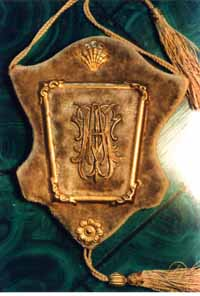
\includegraphics{dcard}}
\caption{\label{dance:card}A 19$^{th}$ Century Hungarian Dance Card}
\end{figure}

In this chapter we will look at a simulated Ball, or at least the dance negotiation part of the Ball. In our simulation we have \mail dancers and \phemail dancers; the \q{mail}s attempt to \emph{mark the card} of as many \phemail{}s as possible. Each \phemail has a preassigned number of slots in her dance card.
\begin{aside}
This is not a very realistic simulation. For one thing, many of the potential partners will already be known to each other; and also in a real Ball there are a fixed number of dance slots and each dancer has the potential to fill dance every dance.
\end{aside}
In order that dance partners can be found, we will have a directory that acts as a general kind of notice board: \phemail{}s publish a description of themselves in the directory and \mail{}s search the directory for potential partners. 

Each \mail agent has the same task -- to find \phemail{}s and to attempt to reserve a dance with them -- as many as possible. Each \phemail agent responds to requests for a dance and either grants it, or, if their dance card is already full, given the suitor a \q{rainCheck}.

Our simulation starts with a fixed number of \mail and \phemail agents, and will stop when all negotiations are complete.

\section{A negotiation protocol}
\label{dance:proto}

One way in which our simulation will be somewhat accurate is in the fact that the various dancers -- both \mail and \phemail -- will be acting as autonomous processes or threads. In order for a successful agreement to have a dance, there needs to be a negotiation between the two dancers. In our simulation, this negotiation is carried out by exchanging messages.

\subsection{Message communication in \go}
\label{dance:mbox}

\index{message communication}
\index{go.mbox@\q{go.mbox} package}
\go has a standard package -- \q{go.mbox} -- that permits threads to send and receive messages. Message communication is a high-level robust way of establishing \emph{coordination} between different threads or processes. It is, in practice, much easier to manage than using the \q{sync}hronized access to shared resources that we saw in Chapter~\ref{directory}.

\go's message communication is based on the \q{mailbox[]} and the \q{dropbox[]} abstractions. The \q{mailbox[]} is used by a thread to read messages that have been sent to it; and the \q{dropbox[]} is used by threads to send messages to its linked \q{mailbox[]}. This model is intended to be a \emph{multiple writers, single reader} communications model -- once the \q{mailbox} is created, its \q{dropbox}es can be distributed to any number of other threads of activity.

\begin{aside}
In principle, it is not required that a given \q{mailbox[]} has just one type of \q{dropbox[]} -- there could be a rich variety of \q{dropbox}es; each targeted at a different mode of message transport. However, \go's standard \q{go.mbox} package only supports a single kind of message communication: oriented towards exchanging messages between threads in a single invocation of the \go engine.
\end{aside}

\index{dropbox@\q{dropbox[]} type}
The interface for a \q{dropbox[]} is straightforward: it has a single main method -- \q{post} -- that permits messages to be delivered to its \q{mailbox[]}. Program~\vref{dance:dropbox} gives the type interface to the standard \q{dropbox[]}.
\begin{program}
\vspace{0.5ex}
\begin{alltt}
dropbox[M] \impl \{ post:[M]* \}.
\end{alltt}
\vspace{-2ex}
\caption{The standard \q{dropbox} type interface}
\label{dance:dropbox}
\end{program}
Notice also that the \q{dropbox[]} type is \emph{polymorphic}. It is polymorphic in the type of the message. Each message communication channel can handle messages of a single type. \go's message communication is strongly typed, just like other aspects of the language.

\index{mailbox@\q{mailbox[]} type}
The interface that a thread has for \emph{reading} messages is encapsulated in the \q{mailbox[]} type interface, shown in Program~\vref{dance:mailbox}. Reading messages is inherently more complex than sending them, and this interface reflects that.
\begin{program}
\vspace{0.5ex}
\begin{alltt}
mailbox[M] \impl \{
  next:[M]*. nextW:[M,number]*. pending:[]\{\}.
  msg:[M]*. msgW:[M,number]*. dropbox:[]=>dropbox[M]
\}.
\end{alltt}
\vspace{-2ex}
\caption{The standard \q{mailbox} type interface}
\label{dance:mailbox}
\end{program}

There are two ways of reading messages from a \q{mailbox}: we can read each message as it comes in -- using the \q{next} action -- or we can \emph{search} the \q{mailbox} for matching messages -- using the \q{msg} action -- which also \emph{blocks} should there be no matching message. Both the \q{msg} and the \q{next} have \emph{timeout} versions -- \q{msgW} and \q{nextW} -- that will only block for a certain time, after that they \q{raise} a \q{timedout} exception.

We find that, for many applications, the \q{msg} oriented approach is often easier to understand and leads to fewer complications; so that is how we shall proceed.

\subsection{Negotiation messages}
\label{dance:message}
\index{negotiation between agents}
In order for the \mail and \phemail agents to understand each other there has to be agreement on the messages communicated. Establishing an algebraic type is an excellent way of defining the messages that flow in a conversation -- especially since \q{mailbox[]}es and \q{dropbox[]}es are themselves typed with the type of the messages that they convey.

In general, \firstterm{conversation}{a conversation is a sequence of messages that occur between two (or more) message exchanging agents.}s are two-way; it is good practice to have two types: one for each \emph{direction} in the conversation (unless, of course, the messages in a conversation can go in either direction). This leads to a style where each conversation has two \q{mailbox/dropbox} pairs -- one pair for each direction in the conversation.

In our Ball simulation, \mail agents propose to \phemail agents, and the latter respond with yeah or nay; so we shall use two types -- as seen in program~\vref{dance:type} -- to reflect the conversations from the different perspectives of the two kinds of agent.
\begin{program}
\vspace{0.5ex}
\begin{alltt}
mailProto::=shallWe(symbol,dropbox[phemailProto]).

phemailProto::=whyNot(symbol,dropbox[mailProto]) | 
                 rainCheck(symbol,dropbox[mailProto]).
\end{alltt}
\vspace{-2ex}
\caption{The message types in the \q{dance} protocol}
\label{dance:type}
\end{program}
The \q{mailProto} type -- used by the \mail agent to propose to a \phemail agent -- has just a single constructor -- \q{shallWe}. This message is used to initiate a proposal dance.

\begin{figure}
\centering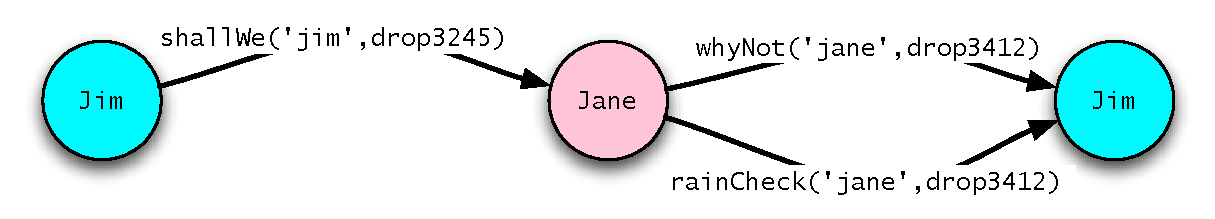
\includegraphics[width=\textwidth]{protocol}
\caption{\label{dance:protocol}A dance negotiation}
\end{figure}

Since our \mail agents don't express a preference for a particular dance, the \q{shallWe} constructor has just two arguments -- a \q{symbol} which is used simply for human readable tracing and a \q{dropbox[]}. The \q{dropbox} will be used by the \phemail agent to reply to the \mail agent. This is a familiar pattern in message-based communication: messages include in them the means of replying.

When a \mail agent sends a \q{shallWe} message to a potential partner, it will execute the \q{post} action on the \q{dropbox} belonging to the \phemail:
\begin{alltt}
\ldots;P.post(shallWe('jim',jimDropBox));\ldots
\end{alltt}
We shall see below how a \mail agent uses the directory to acquire a \phemail's \q{dropbox}; of course \q{jimDropBox} is its own \q{dropbox} -- which every agent should have easy access to.

To \emph{receive} the \q{shallWe} message, the \phemail agent executes a \q{msg} action, using its \q{mailbox}:
\begin{alltt}
\ldots;ourBox.msg(shallWe(Who,Rep));\ldots
\end{alltt}
A successful completion of this action would result in the \q{Who} and \q{Rep} variables being bound to the name of the proposer and its \q{dropbox}. Below, we shall see how the \phemail deals with the message.

There are two constructors in the \q{phemailProto} type -- the \q{whyNot} and the \q{rainCheck} constructors. The former is used by a \phemail when accepting a proposition and the \q{rainCheck} is used when rejecting it.

These constructors follow the same pattern as the \q{shallWe} constructor; but as the potential conversations between Ballroom agents are very short the true role of the \q{dropbox[]} argument in the \q{whyNot} and \q{rainCheck} messages is slightly different: to allow the \mail to \emph{confirm} that the reply message to its \q{shallWe} proposal is from the expected \phemail. Of course, there are other ways of doing this -- such as using a randomly generated number as a key.


In addition to the \q{mailProto} and \q{phemailProto} types, it is convenient to have two \q{attVal} classes for encapsulating the \q{dropbox[]}es of the two kinds of dancer:
\begin{alltt}
locM:[dropbox[mailProto]]\conarrow{}attVal.
locM(_)<=thing.

locF:[dropbox[phemailProto]]\conarrow{}attVal.
locF(_)<=thing.
\end{alltt}
We will use these constructors to publish and search the ballroom's directory for appropriate partners.


\begin{aside}
A more elaborate conversation protocol would almost certainly have a richer collection of message types. In addition, each message would carry more information. One immediate thought for a suitable extension would be the name of the particular dance being proposed and/or disposed. For example, a \mail agent might propose the first Waltz, and the \phemail might respond with an acceptance for the second Polka. However, we leave aside such elaborations in this example.
\end{aside}

\section{A \mail agent}
\label{dance:mail}

The task of the \mail agent is to locate as many \phemail agents as possible and to propose to dance with them. We might express this as the iteration:
\begin{alltt}
P in Phemails *> propose(P)
\end{alltt}
except that it may be useful to collect information about the \phemail agents it encounters (after all, negotiation is but the first step in the dance). So, the heart of our \mail dancer is the computation of the bounded set expression:
\begin{alltt}
\{ P .. (P::propose(P)) in Phemails \}
\end{alltt}
where \q{propose} is a predicate that is satisfied for every successful proposal to a \phemail agent. Recall that an expression such as:
\begin{alltt}
P::propose(P)
\end{alltt}
is a \emph{guarded pattern}, and, in this case, denotes a \q{P} which is a member of the list \q{Phemails} for which \q{propose} is satisfied.

In a successful negotiation, the \mail agent must first send a \q{shallWe} message to the \phemail, and must receive a \q{whyNot} message in reply. Of course, it is possible that the reply is a \q{rainCheck}, in which case there will be no dance.

This is an instance where the success of a predicate -- \q{propose} -- depends on the results of a sequence of \emph{actions}. \go has mechanisms for relating actions to expressions and predicates: we saw a use of the \q{valof/valis} combination in Program~\vref{directory:package}. For predicates we have the \q{action} predicate condition: an \q{action\{\}} condition wraps an action sequence as a way of satisfying a predicate.

\subsection{A \mail proposal}

\index{action@\q{action} query}
To satisfy a \q{propose}, we need to send a message and receive a reply; we can do this with the relation definition:
\begin{alltt}
propose:[dropbox[mailProto]]\{\}.
propose(P) :- action\{
    P.post(shallWe(ourName,ourDrop));
    ourBox.msg(Reply);
    istrue whyNot(H,\_).=Reply
  \}.
\end{alltt}
where we are assuming some auxiliary definitions: \q{ourName} and \q{ourDrop} are the symbolic names of this \mail dancer and its \q{dropbox} respectively and \q{ourBox} is its \q{mailbox}. The argument to \q{propose} is directly a \q{dropbox}.

The form:
\begin{alltt}
action\{ \ldots istrue \emph{Condition} \ldots\}
\end{alltt}
is the query analogue of the \q{valof}/\q{valis} expression condition. The action
\begin{alltt}
istrue whyNot(H,\_).=reply
\end{alltt}
determines the truth value associated with the \q{action} itself. If the query condition
\index{match query}
\index{operator!.=@\q{.=}}
\begin{alltt}
whyNot(H,\_).=reply
\end{alltt}
is satisfied, then the truth value will be \q{true} and the \q{action} will succeed also.

This query condition represents a \emph{match} of the pattern \q{whyNot(H,\_)} against the variable \q{Reply}. This is the same kind of matching that is used in the head of an action rule against the arguments of the action -- and in the head of an equation against the function call. In this case the match succeeds if \q{Reply} is \emph{already} bound to a value of the form \q{whyNot(H,\_)} -- i.e., the match may not bind \q{Reply} -- although it may bind variables on the left hand side of the condition. The second variable in the \q{whyNot(H,\_)} pattern is \emph{anonymous} and no-one cares what its values is anyway, but the first is used to collect names of dance partners.

\subsection{A \mail class}
\index{mail@\q{mail} class}
When we build our ballroom, we will want the various dancer agents to execute in parallel -- to reflect their autonomous nature. We expect our dance agents to carry some \emph{state} -- in particular a record of the dance partners that they have agreed to dance with. On the other hand, that state is essentially \emph{private} to the dancers and should not be unnecessarily exposed. Although \q{mail} and \q{phemail} dancers are quite different internally, from a top-level perspective they should be managed in the same way within the simulation.

To regularize this, we propose a \q{dancer} interface that the top-level simulation uses to \q{spawn} and otherwise control the dancers and each dancer agent -- \mail and \phemail -- will be expected to implement that interface:
\begin{alltt}
dancer \typearrow{} \{ start:[]*. report:[]=>string \}
\end{alltt}
The \q{start} action will be invoked when the dancer agent is expected to start executing -- we should of course also have a \q{stop} action. The \q{report} function is there to permit the top-level simulation to request a report on the status of each dancer.

In Program~\vref{dancer:mail} we wrap up the \mail agent in a class body -- that implements this \q{dancer} interface type -- including some of the auxiliary definitions hinted at above. Since the \mail is a stateful entity we use the \sconarrow{} class constructor in establishing the type of the \mail class.

Note that \q{explode} -- it is used in the \q{report} function -- is a standard library function that is used here to convert the \q{Name} \q{symbol} into a \q{string}.

\begin{program}[bt]
\vspace{0.5ex}
\begin{alltt}
mail:[symbol]\sconarrow{}dancer.
mail(ourName)..\{
  ourBox:mailbox[phemailProto] = mailbox.
  ourDrop:dropbox[phemailProto] = ourBox.dropbox().
  partners:list[symbol] := [].

  propose:[dropbox[mailProto],symbol]\{\}.
  propose(P,H) :- action\{
     P.post(shallWe(ourName,ourDrop));
     ourBox.msg(Reply);
     istrue whyNot(H,_).=Reply
   \}.

  Phemails:[]=>list[dropbox[mailProto]].
  Phemails() => \{ locOf(A) .. A in 
     dir.find([at('gender',aG(female))],['loc']) \}.

  locOf:[list[attr]]=>dropbox[mailProto].
  locOf(A) :: at('loc',locM(P)) in A => P.

  start() -> 
     partners := \{ H..(P::propose(P,H)) in Phemails() \}.

  report() => explode(Name)<>" with "<>partners.show().
\}
\end{alltt}
\vspace{-2ex}
\caption{A \mail dancer class}
\label{dancer:mail}
\end{program}

The \q{Phemails} function queries the shared directory to locate descriptions that have a \q{'gender'} attribute of \q{female}. The \q{dropbox} of the \phemail agent is extracted from the description using the \q{locOf} auxiliary function.

\subsubsection{Assignment in a class}
\index{class!assignment in}
The \q{start} action procedure has an \emph{assignment} within it:
\begin{alltt}
partners := \{ P..(P::propose(P)) in Phemails() \}
\end{alltt}
Assignment is permitted for special re-assignable variables declared in a class body; in the case of the \q{partners} variable its declaration was:
\begin{alltt}
partners:list[symbol] := [].
\end{alltt}
\go supports reassignable variables, but with some restrictions: their values must be ground -- they may not have any unbound variables within their value -- and they are \emph{private} to a class body or package. In particular, they may not be re-assigned outside the context that they are declared. For variables declared in a class body, that means that only rule programs defined in the same class body may modify their values. Finally, only stateful classes -- introduced with the \sconarrow{} class constructor type -- are permitted to define constants and variables in their class body.

These restrictions are there partly to permit reasonable implementations and partly to control the implications of having a re-assignable variable. Ensuring that only programs defined in the same scope may modify variables means that program analysis is that much simpler. It also means that it is not possible for a programmer to subtly change the semantics of a variable defined in a super class.

Program~\vref{dancer:mail} also has a \emph{constant} definition within it:
\begin{alltt}
  ourDrop:dropbox[phemailProto] = ourBox.dropbox().
\end{alltt}
\q{ourDrop} is a constant because, once its value is established, it cannot be overwritten with a new value -- unlike variables. 

An object constant like this is established every time an instance of the \mail class is created. Thus every time we evaluate the constructor expression \q{mail(\emph{Name})} a new \q{ourBox} is also created, and a new copy of \q{ourDrop} established.

\section{A \phemail agent}
\label{dance:phemail}

\index{phemail@\phemail class}
The \phemail agent is the counterpart of the \mail agent; its heart is an action that waits for \q{shallWe} messages from proposing \mail agents and responds to those messages. This is preceded by an initialization phase in which the \phemail posts a description of itself with the shared directory.

\index{directory!registering with}
The simplest description consists of the \q{name} of the agent, its \q{gender} and, critically, the \q{dropbox} that the \mail agents can use to contact the \phemail:
\begin{alltt}
init() -> dir.register([at('name',aS(Name)),
                        at('gender',aG(female)),
                        at('loc',locM(ourDrop))]).
\end{alltt}
Note that although the \phemail agent publishes its name, the \mail agent is not actually interested in the name. This is a common scenario: agents that publish descriptions of themselves will often \emph{over-describe} themselves -- it is difficult to predict the actual uses of services ahead of time. The flexibility of the attribute/value style of descriptions makes this over-description harmless.

\begin{program}[h]
\vspace{0.5ex}
\begin{alltt}
phemail:[symbol,integer]\sconarrow{}dancer.
phemail(Nme,Limit)..\{
  ourBox:mailbox[mailProto] = mailbox.
  drop:dropbox[mailProto] = ourBox.dropbox().
  partners:list[symbol] := [].

  init() -> dir.register([at('name',aS(Nme)),
                          at('gender',aG(female)),
                          at('loc',locM(drop))])
  
  accepting:[integer]*.
  accepting(Count)::Count>0 ->
    ourBox.msg(shallWe(Who,Rep));
    Rep.post(whyNot(Nme,drop));
    partners := [Who,..partners];
    accepting(Count-1).
  accepting(0) -> rejecting().

  rejecting:[]*.
  rejecting() -> ourBox.msg(shallWe(_,Reply));
    Reply.post(rainCheck(Nme,ourBox));
    rejecting().

  start() -> init(); accepting(Limit).

  report() => explode(Nme)<>" with "<>partners.show().
\}
\end{alltt}
\vspace{-2ex}
\caption{A \phemail dancer class}
\label{dancer:phemail}
\end{program}

If we assume that each \phemail has a predefined limit of how many partners it can accept then the main loop of the agent can be captured in two action procedures \q{accepting} for when the \phemail is accepting proposals and \q{rejecting} for when it is not. This is achieved in Program~\vref{dancer:phemail} by using two recursive action procedures -- \q{accepting} and \q{rejecting}. When in the \q{accepting} procedure, the dancer is potentially accepting new proposals; when there is no more room, the \q{accepting} action procedure calls the \q{rejecting} procedure -- which never accepts any proposals.

The \q{accepting}/\q{rejecting} pair of action procedures make, in effect, a simple state machine. State machines are a common technique for constructing simple agents; although more complex behaviors require more sophisticated approaches.

\section{The Ballroom}
\label{dance:ballroom}
The final piece of our simulation is the ballroom itself; or the top-level driver of the simulation. At the top-level we model each \q{dancer} as a separate thread of activity, as well as another thread for the \q{directory}. 

The main phases of the simulation driver are an initialization phase -- where the different agents are created and \q{spawn}ed off -- a waiting phase and the final reporting phase.

Managing a \q{spawn}ed off activity can be challenging: we need to be able to coordinate with it and to potentially kill it off or wait for it to terminate. 

\index{expression!spawn@\q{spawn}}
We have seen that \q{spawn} is an action; it is also an \emph{expression}. The value returned by a \q{spawn} expression is the thread identifier of the new activity -- of type \q{thread}. This value can be used to determine the state of the thread, or otherwise manage it: the \q{kill} function terminates a thread and the \q{waitfor} action procedure suspends until the thread has terminated (naturally or not).

For our purposes we will \q{spawn} a number of \mail threads of activity and \phemail threads. The latter do not have a natural termination as a \phemail cannot know if there are more \mail{}s to propose. On the other hand, a \mail agent, as we have written it in program~\vref{dance:mail}, does terminate once it has proposed to all the \phemail{}s it finds from the directory.

We can use this termination as a way of deciding when the simulation should enter its final reporting phase:
\begin{alltt}
\ldots ( M in \emph{MailThreads} *> waitfor(M)); \ldots
\end{alltt}
\index{forall!action}
\index{operator!*>@\q{*>}}
This uses the \emph{forall} operator -- \q{*>} -- as an action; we have already seen its use as a predicate condition in program~\vref{directory:directory}. In this case we iterate over the known \mail threads, waiting for each to finish. When they are all ended we assume that the simulation has stabilized.

\begin{program}[tb]
\vspace{0.5ex}
\begin{alltt}
main(_) ->
  stdout.outLine("Starting...");
  Phems = [ phemail('jill',1),phemail('jane',2),
            phemail('joan',3),phemail('jenny',4)];
  (F in Phems *> spawn\{F.start()\});
  Mails = \{ mail(N) .. N in ['fred','jim','peter',
                              'alfred','john'] \};
  (M in \{ spawn\{ MM.start()\} .. MM in Mails\}*>waitfor(M));
  stdout.outLine("Reporting...phems...");
  (F in Phems *> stdout.outLine(F.report()));
  stdout.outLine("Reporting...mayls...");
  (M in Mails *> stdout.outLine(M.report())).
\end{alltt}
\vspace{-2ex}
\caption{Top-level of Ballroom simulation}
\label{dance:main}
\end{program}

A complete top-level main program is shown in program~\vref{dance:main}; inevitably, this \q{main} program has something of the character of a sequential script: starting programs off, waiting for them to finish, collecting information. A sample run of our ballroom simulation looks like:
\begin{alltt}
Starting...
Reporting...phems...
jill with ['fred']
jane with ['jim','fred']
joan with ['peter','jim','fred']
jenny with ['alfred','peter','jim','fred']
Reporting...mayls...
fred with ['jill','jane','joan','jenny']
jim with ['jane','joan','jenny']
peter with ['joan','jenny']
alfred with ['jenny']
john with []
\end{alltt}

\section{Summing up}
So far, we have seen a little of the style and programming power of the programming language \go. The ballroom simulation is a fairly complex program that would take many times as much space in some other programming languages. Yet, for the most part, it is also quite an elegant program and we are not over-burdened with a lot of minor details.



\addtocontents{lop}{\protect\addvspace{1ex}}
\chapter{Programming interpreters}
\label{meta}

\index{meta programming techniques}
\lettrine[nindent=0.1em]{A}{number of programming techniques} rely on or can be considered to be variations of \firstterm{meta programming}{A style of programming that leverages the relationship between the name or description of an entity and the entity itself. A common use of meta-programming is the \emph{interpreter}; which is a program that interprets a data structure that represents a program, allowing computation with that represented program. Another common example is the use of `class of' operators that allow introspection of objects.}. Meta programming is a style of programming that leverages the relationship between the name or description of an entity and the entity itself. A common meta-programming example is the interpreter; which is a program that interprets a data structure that represents a program, allowing computation with that represented program. Another common example is the use of `class of' operators that allow introspection of objects. In this chapter we explore how to build an \emph{interpreter} for a very simple logic-like language in \go.

\section{A simple logic language}
Our simple logic language is a variant of horn-clause logic: a program consists of clauses, each clause is of the form of a `body' and a `head'; the interpretation of this being that if the body is satisfied then the head is also satisfied. 

Note that since \go is a strongly typed language, we would like to extend this also to our interpreted language. I.e., even though our language is intended to be interpreted, for it to integrate smoothly with \go it is necessary to be equally rigorous about types. We can do this and still maintain generality by using different classes to implement the different kinds of logical formulae, all sharing a common type -- \q{metaTp}.

\subsection{Representing language elements}
\index{representing logical formulae}
\label{meta:type}
In order to interpret a data structure as a language we need to \emph{represent} elements of the language as \go structures. In the case of our logic language we need to be able to represent rules, conditions, terms and so on. One way of doing this could be to use constructors for each of possible elements, for example to use a term
\begin{alltt}
conj([ C\sub1, \ldots, C\subn])
\end{alltt}
to represent a conjunction. The definition of these constructors might take the form of a algebraic type definition:
\begin{alltt}
metaTp[CT] ::=  conj(list[metaTp[CT]]) | \ldots
\end{alltt}
A slightly more paradigmatic approach is to define an \emph{interface} for rules and conditions, and then to define classes that implement the interface. In the case of a condition, the immediate interface requirement is to be able to \emph{evaluate} the condition; in the case of a logic language evaluation is expressed primarily as \q{satisfy} -- solving queries. We detail this interface in program~\ref{meta:interface}.
\begin{program}
\vspace{0.5ex}
\begin{alltt}
meta\{
  metaTp \impl \{ satisfy:[]\{\} \}.
  ...
\}
\end{alltt}
\vspace{-2ex}
\caption{The interpreter interface}
\label{meta:interface}
\end{program}

With this type interface we can begin to define classes that implement the \q{metaTp} interface. For example, the \q{conj} class is detailed in program~\vref{meta:conj}.
\begin{program}
\vspace{0.5ex}
\begin{alltt}
conj:[list[metaTp]]\conarrow{}metaTp.
conj(C)..\{
  satisfy() :-
    solve(C).
  
  solve:[list[metaTp]]\{\}.
  solve([]).
  solve([G,..R]) :- G.satisfy(), solve(R).
\}
\end{alltt}
\vspace{-2ex}
\caption{The \q{conj} class}
\label{meta:conj}
\end{program}
An interesting feature of \q{satisfy} in the definition of \q{conj} is that it uses the label argument \q{C} from the class label to \emph{carry} the data. We can see this if we look at a typical call to \q{satisfy} using a \q{conj} label:
\begin{alltt}
conj([\emph{C\sub1},\ldots,\emph{C\subn}]).satisfy()
\end{alltt}
The list of \emph{C\subi} represents conditions to satisfy; within the \q{conj} class these conditions are held in the label argument \q{C}. Of course, this is just how one might use \prolog terms to represent interpreted programs. However, \prolog cannot easily combine this with the invocation of programs the way that we can use classes in \go.

The class definitions for the disjunctive case -- \q{disj} -- and negation -- \q{not} -- are directly analogous to the \q{conj} class. The only difference is in the definitions of \q{satisfy} within each class. Program~\vref{meta:disnot} contains, for reference, these classes.
\begin{program}
\vspace{0.5ex}
\begin{alltt}
disj:[list[metaTp]]\conarrow{}metaTp.
disj(C)..\{
  satisfy() :-
    G in C, G.satisfy().
\}.

not:[metaTp]\conarrow{}metaTp.
not(C)..\{
  satisfy() :-
    \nasf{} C.satisfy().
\}
\end{alltt}
\vspace{-2ex}
\caption{Disjunction and negation}
\label{meta:disnot}
\end{program}

The class for implementing rules is not a great deal more complex than those for the query types. The main technique required is to represent calls to interpreted rule programs with their class label -- \q{ask} -- in our version; and to rely on a repository for the rules themselves.
\begin{program}
\vspace{0.5ex}
\begin{alltt}
ask:[metaTp]\conarrow{}metaTp.
ask(P)..\{
  satisfy() :-
    isRule(P,Body),
    Body.satisfy().
\}.
\end{alltt}
\vspace{-2ex}
\caption{Interpreted rules}
\label{meta:rule}
\end{program}
The \q{isRule} relation mentioned in program~\vref{meta:rule} represents the main repository of interpreted rules. Given that we are interpreting programs, it is likely that this repository is itself represented using \q{dynamic} relations which we have already seen used to store descriptions in a directory in program~\vref{directory:directory}. 

\subsection{Escaping into regular \go}
An interpreter for any language has to handle two fundamental aspects of the language: how composite elements are interpreted -- in our case these are disjunction, conjunction and so on -- and how primitive elements are interpreted. These primitive elements may be like \emph{escapes} -- that invoke functionality directly from \go.\note{The \go engine itself has escapes that invoke ``C'' code for executing operating system functions such as reading and writing to files.}

Our escape technique reflects the inherent extensibility of \go's object oriented system. All that is really required is that each primitive is represented by a class that realizes the \q{metaTp} type. We illustrate this in program~\vref{meta:plus} with a pseudo-logical primitive -- \q{plus} -- which implements arithmetic.
\begin{program}
\vspace{0.5ex}
\begin{alltt}
plus:[integer, integer, integer]\conarrow{}metaTp.
plus(A,B,C)..\{
  satisfy() :-
    C = A+B.
\}.
\end{alltt}
\vspace{-2ex}
\caption{Intepreted addition}
\label{meta:plus}
\end{program}

We can use a \q{plus} condition in a query in much the same way as we would use a \q{conj} condition, the main difference being that the arguments of \q{plus} are numeric:
\begin{alltt}
conj([plus(1,2,x),conj([plus(2,1,x)])]).satisfy()
\end{alltt}

\section{Dynamic family relationships}
\label{meta:family}
If we were representing -- in \go -- some simple genealogical relations between people, such as who is the parent of who, then we might expect to be able to use rules such as
\begin{alltt}
parent:[symbol,symbol]\{\}
parent('j','k').
parent('k','l').
\end{alltt}
We have some flexibility in how we represent such data so that our interpreter system can reason genealogically. We could, for example, throw everything into a single \q{dynamic} relation and fetch individual facts as needed. However, that seems clumsy.

\subsection{Dynamic relations}
\index{representing dynamic relations}
One effective of incorporating dynamic relations into our interpreted system is to use a \emph{paired} approach -- to construct a pair consisting of a \q{parent} class with the normal \q{metaTp} type interface, and a separate parallel \q{Parent} entity that realizes a \q{dynRel} type that supports an \q{assert} interface.\note{The \q{mailbox[]}/\q{dropbox[]} pair in the \q{go.mbox} package -- discussed in Section~\vref{dance:mbox} -- is another example of this kind of pairing.}

Program~\vref{meta:ppackage} shows an example of this for the \q{parent} relation and its \q{Parent} paired \q{dynamic} set.

\begin{program}
\vspace{0.5ex}
\begin{alltt}
parent\{
  import meta.
  import dynamicRel.
  
  Parent:dynRel[(symbol,symbol)] = dynRel([]).
  
  parent:[symbol,symbol]\conarrow{}metaTp.
  parent(A,B)..\{
    satisfy() :-
      Parent.mem((A,B)).
  \}.
\}.
\end{alltt}
\vspace{-2ex}
\caption{Parent package}
\label{meta:ppackage}
\end{program}

To query the \q{parent} relation, we use the same queries as for non-dynamic relations:
\begin{alltt}
parent('jim','bill').satisfy()
\end{alltt}
to represent queries to the \q{parent} relation.
To modify the relation, perhaps to record a new birth, we use actions of the form:
\begin{alltt}
Parent.assert(('jim','joe'))
\end{alltt}

\begin{aside}
Note that, although, in program~\vref{meta:ppackage}, we can modify the \q{parent} relation -- through the \q{assert} and \q{retract} methods on the associated \q{Parent} --  this is still not the same as \prolog's assert and retract primitives.

The reason is that our interpreted rules cannot invoke these methods as part of the query evaluation. Of course, the application in which the meta-system is embedded can modify the dynamic relations. This separation is enough to ensure logical soundness of the interpreter -- assuming that the main query evaluation procedure is sound.
\end{aside}

The \q{dynamicRel} class is a straightforward use of the \q{dynamic} class, and is shown in Program~\vref{meta:dynamic}.

\begin{program}
\vspace{0.5ex}
\begin{alltt}
dynamicRel\{
  import go.dynamic.

  dynRel[T] \impl{} \{ assert:[T]*. retract:[T]* \}.
  dynRel[T] \impl{} dynamic[T].

  dynamicRel:[list[T]]\sconarrow{}dynRel[T].
  dynamicRel(I) <= dynamic(I).
  dynamicRel(_)..\{
    assert(X) ->
        add(X).
    retract(X) ->
    	    del(X).
  \}.
\}.
\end{alltt}
\vspace{-2ex}
\caption{Dynamic interpreted relations}
\label{meta:dynamic}
\end{program}

\subsection{Family ancestors}
\label{meta:ancestor}
Not all interpreted relations are \emph{flat} -- some are better expressed as recursive rules. For example, the ancestor relation might be defined in regular \go as:
\begin{alltt}
ancestor:[symbol,symbol]\{\}.
ancestor(X,Y) :- parent(X,Y).
ancestor(X,Y) :- parent(X,Z), ancestor(Z,Y).
\end{alltt}
We could incorporate such a recursive rule into our interpreted system in the same way that we incorporated \q{plus} in Program~\vref{meta:plus}. However, we can also \emph{interpret} ancestors; supporting dynamic rules in an analogous way that we supported dynamic relations. 

\begin{program}[bt]
\vspace{0.5ex}
\begin{alltt}
dynamicRules\{
  import go.dynamic.
  import meta.

  dynRule[T] \impl \{ assert:[T,metaTp]*. satisfy:[T]\{\} \}.
  dynRule[T] \impl dynamic[T].

  dynamicRule:[list[T]]\sconarrow{}dynRule[T].
  dynamicRule(I) <= dynamic(I).
  dynamicRule(_)..\{
    satisfy(X) :-
        mem((X,B)),
        B.satisfy().
    assert(X,B) ->
        add((X,B)).
  \}.
\}.
\end{alltt}
\vspace{-2ex}
\caption{Interpreted rules}
\label{meta:rules}
\end{program}

Program~\vref{meta:rules} is a package that is similar to the package in Program~\vref{meta:dynamic}; oriented to handling rules. Like that program, we define a new interface for handling dynamic rule programs. The \q{dynRule[]} type has a \q{satisfy} element, as well as an \q{assert} element to simplify the paired rule programs. 

\begin{program}[bt]
\vspace{0.5ex}
\begin{alltt}
ancestor\{
  import meta.
  import dynamicRules.
  import parent.

  Ancestor:dynRule[(symbol,symbol)]=
      dynamicRule([((A,B),parent(A,B)),
                   ((A,C),conj([parent(A,B),
                                ancestor(B,C)]))]).

  ancestor:[symbol,symbol]\conarrow{}metaTp.
  ancestor(A,B)..\{
    satisfy() :- Ancestor.satisfy((A,B)).
  \}.
\}
\end{alltt}
\vspace{-2ex}
\caption{Interpreted ancestry}
\label{meta:dynamic:ancestor}
\end{program}

The \q{satisfy} relation definition in the \q{dynamicRule} class uses \q{mem} to find a rule -- represented as a pair consisting of a head and a body. The body is a \q{metaTp} term, which is queried by invoking \q{satisfy} on that term. 

The definition of \q{ancestor} in program~\vref{meta:dynamic:ancestor} shows how we can use the \q{dynamicRule} class to establish the rules of ancestry.

\index{variable!in \q{dyamic} relations}
\index{dynamic@\q{dynamic} relation!variables in}
A sharp observer might wonder how \emph{variables} are managed in the representation of the rules for \q{ancestor}. Normally, assignable values are required to be \emph{ground}; which clearly will not permit us to represent rules such as for ancestor. However, the \q{dynamicRules} package relies on the standard \q{go.dynamic} package. This package implements a subtly different semantics for assignment.

In a \q{dynamic} relation, the entries are generally tuples. When a tuple has one or more variables in it then, whenever that tuple is retrieved from the \q{dynamic} relation -- typically by way of the \q{mem} predicate method -- the variables in the tuple are \emph{refreshed} each time. That means that the tuple is \emph{copied} and any variables replaced with new ones. Thus each time a tuple is retrieved from the \q{dynamic} relation, it will have different variables in it. 

This refreshment, which in logic is called \emph{standardizing apart}, is how we are able to use a \q{dynamic} relation to store the rules for the recursive \q{ancestor} program without getting the variables in it confused.

\section{Family trees}
\label{meta:family:tree}

\begin{figure}[bt]
\centerline{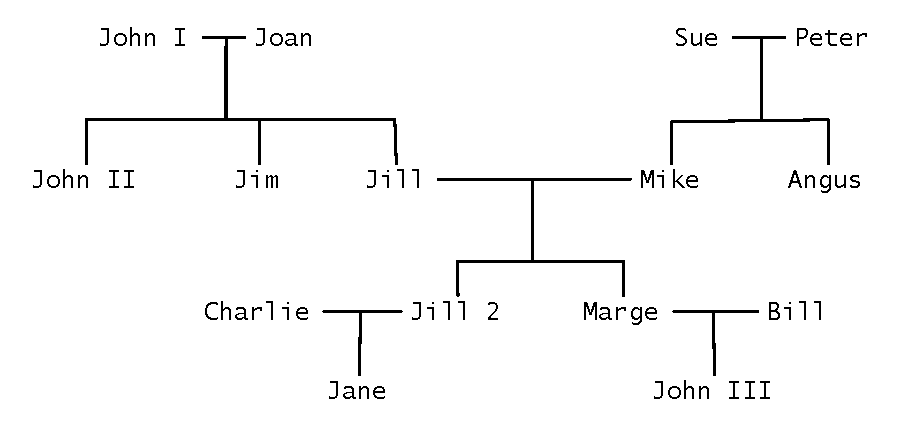
\includegraphics[width=0.8\textwidth]{familytree}}
\caption{\label{meta:tree}A family tree}
\end{figure}

We are finally in a position to put together a complete family tree and to try some queries against it. Figure~\vref{meta:tree} shows a small family tree with three generations displayed. Such a tree can be set up using the program \q{defineTree} in program~\vref{meta:family:setup}.


\begin{program}
\vspace{0.5ex}
\begin{alltt}
buildTree() ->
    Parent.assert(('John I','John II'));
    Parent.assert(('John I','Jim'));
    Parent.assert(('John I','Jill'));
    Parent.assert(('Joan','John II'));
    Parent.assert(('Joan','Jim'));
    Parent.assert(('Joan','Jill'));
    Partner.assert(('John I','Joan'));
    Partner.assert(('Peter','Sue'));
    Parent.assert(('Peter','Mike'));
    Parent.assert(('Peter','Angus'));
    Parent.assert(('Sue','Mike'));
    Parent.assert(('Sue','Angus'));
    Partner.assert(('Mike','Jill'));
    Parent.assert(('Mike','Jill 2'));
    Parent.assert(('Mike','Marge'));
    Parent.assert(('Jill','Jill 2'));
    Parent.assert(('Jill','Marge'));
    Partner.assert(('Charlie','Jill 2'));
    Parent.assert(('Charlie','Jane'));
    Parent.assert(('Jill 2','Jane'));
    Partner.assert(('Bill','Marge'));
    Parent.assert(('Marge','John III'));
    Parent.assert(('Bill','John III')).
\end{alltt}
\vspace{-2ex}
\caption{Interpreted family tree}
\label{meta:family:setup}
\end{program}

Evaluating a query against this family tree amounts to invoking the \q{satisfy()} predicate of a suitable term. For example, to list all the descendants of \q{'John I'}, we can use the forall iterator:
\begin{alltt}
(ancestor('John I',Y).satisfy() *>
  stdout.outLine("John I ancestor of "<>Y.show()))
\end{alltt}
Or to display the ancestors of \q{'Angus'}, we might use:
\begin{alltt}
(ancestor(A,'Angus').satisfy() *>
  stdout.outLine(A.show()<>"is an ancestor of Angus"))
\end{alltt}

The various labeled terms and support packages that we have introduced in this chapter mark a very convenient technique for representing interpreted programs. Of course, for a \emph{given} interpreted program, such interpretation might be over-kill -- especially for a logic program. However, the true semantics of query interpretation comes from the various implementations of \q{satisfy()} in the various classes. We can define and implement an interpreter for any language; simply by having a different kind of \q{eval}uation (say) and a similar set of support classes.

One of the nice features of the approach outlined here is the smooth integration that is possible between an interpreted program and a regular, compiled, \go program. It is straight forward for a \go program to invoke the interpreted program and similarly vice-versa.


\addtocontents{lop}{\protect\addvspace{1ex}}
%\chapter{Planning with STRIPS}
\label{strips}

A key element of many agent applications is the planning of a sequence of actions. This is often broken down into two phases: constructing a plan and executing it. These are related in that often well intentioned plans do not work as advertised; and therefore when executing a plan the preconditions for some or all of the actions may need to be verified, and re-planning may be required. 

In this chapter we look at implementing one of the classic approaches to planning -- namely a STRIPS planner. The STRIPS style of planner assumes a world of discrete actions, discrete goals and observable properties of the world. Each action is characterized by the set of facts that it `adds' to the world -- i.e., makes true if the action is successful -- and the set of facts that it deletes -- i.e., makes false if the action is unsuccessful. Each action is also associated with a set of pre-conditions -- observed properties of the world that must be true for the action to have meaning.

For example, in the blocks world, picking up a block requires that the block is clear -- no block is stacked on top of it -- and that its on the table. If the pickup is successful, then it will no longer be on the table, and will no longer be clear -- in the sense that its not possible to stack blocks `in the hand'; and so \q{clear} really means that it is permitted to stack a block on top of it.
\begin{aside}
Another key assumption in the STRIPS model is that there are no other active agents in the world that can also act. This assumption is clearly invalidated in any multi-agent scenario; however, for an agent planning its internal activities the single-actor assumption is often reasonable.
\end{aside}

\section{Robbie's world of blocks}
\label{strips:blocks}
Our demonstration of our planner is the classic one of a robot -- called Robbie -- being able to manipulate blocks: by picking them, stacking and unstacking and so on.
\begin{aside}
This world should not be confused with anything realistic. However, it's primary purpose here is show how knowledge about a specific domain is integrated with a generic planning engine.

For example, we do not attempt to address how Robbie might be able to perceive that a given block is stacked on another. This is a non-trivial problem, requiring typically the ablity to interpret a scene via a video camera.
\end{aside}
For the simple blocks world the \q{blockActs} type captures the range of available actions:
\begin{alltt}
blockActs ::= stack(symbol,symbol)
    | unstack(symbol,symbol)
    | pickup(symbol)
    | putdown(symbol).
\end{alltt}
we use symbols to identify the various blocks we may encounter.

The \q{blockPred} type names the possible predicates in the blocks world:
\begin{alltt}
blockPred ::= clear(symbol)
    | holding(symbol)
    | ontable(symbol)
    | on(symbol,symbol)
    | handempty.
\end{alltt}
In effect, we are limited to sensing whether a block is \q{clear}, whether it is on the table and so on. Other potentially important properties of blocks, such as their shape, size, weight, color and so on, are not modeled here. Although it would be a relatively simple extension to do so, the art of designing and effective system lies as much in what we \emph{do not} design as in what we do construct.

Just as we simplify the potential properties of blocks, the possible actions that the execution engine (a.k.a. blocks world robot) can take is also simplified: it is possible to stack blocks on top of each other, to unstack a block from a stack, to pick up a block, and to put it on the table. These actions are quite high-level from the perspective of a physical device manipulating real blocks; these actions would have to be broken down into simpler activations of the robot's mechanical muscles.

\subsection{The \q{stripsWorld} interface}
\label{strips:world}
The \q{stripsWorld} type definition:
\begin{alltt}
stripsWorld[A,G] \impl \{
  strips_rule:[A,list[G],list[G],list[G]]\{\}.
\}.
\end{alltt}
expresses the contract that the domain-specific part of the system must fulfill. In order for the generic planner to be able to know what the legal operations are in a given domain, it is given a class that implements this type. The \q{strips\_rule} predicate defines the planning operators themselves.

Note that \q{strips\_rule} is a predicate and not a function because a given set of goals may have more than one action associated with it. It is not permissible for the same action to be mentioned in more than one \q{strips\_rule} clause: that would imply that the action had more than one set of preconditions and consequences.

\subsection{The blocks planning domain}
Our \q{robbie} class, in Program~\vref{strips:robbie}, captures Robbie's possible actions in the world as rules in the \q{strips\_rule} relation.
\begin{program}
\vspace{0.5ex}
\begin{alltt}
robbie\{
  import go.setlib.
  import strips.

  robbie:[]\conarrow{}stripsWorld.
  robbie..\{
    strips\_rule(stack(X,Y),
              [clear(Y),holding(X)],
              [on(X,Y),clear(X),handempty],
              [clear(Y),holding(X)]).
    strips\_rule(unstack(X,Y),
              [on(X,Y),clear(X),handempty],
              [clear(Y),holding(X)],
              [on(X,Y),clear(X),handempty]).
    strips\_rule(pickup(X),
              [ontable(X),clear(X),handempty],
              [holding(X)],
              [ontable(X),clear(X),handempty]).
    strips\_rule(putdown(X),
              [holding(X)],
              [ontable(X),clear(X),handempty],
              [holding(X)]).
  \}.
\}
\end{alltt}
\vspace{-2ex}
\caption{Operators in Robbie's world}
\label{strips:robbie}
\end{program}
Each \q{strips\_rule} in the \q{robbie} class defines the preconditions of the action, the positive effects on the world and the negative effects. For example, the \q{stack} action requires that the block is in the hand of the robot and that the target is \q{clear}. The positive effects are that the newly stacked block is \q{clear} and that the robot's hand is empty. The negative effects are that the target block is no longer \q{clear} and that the robot is no longer \q{holding} the stacked block.\note{For the sake of clarity and simplicity we have assumed that the planner will only plan using primitive actions.}

Although the modeled world of blocks is not permitted to contain predicates with variables, there is no such restriction on the description of the action rules; nor on possible descriptions of the modeled world. This permits \go's descriptions of the possible actions to be very compact; while at the same time simplifying the logic of the modeled world.

Other domains would have different actions, with a different language of conditions. For example, an application in terms of eCommerce might have actions around searching for suitable vendors and purchasing goods.

Note that Program~\vref{strips:robbie} defines the range of actions as a `fixed' relation; but there is nothing intrinsic in this. One might wish to extend this to include a more dynamic, learnable, range of actions.

\section{A simple STRIPS planner}
\label{strips:strips}

Program~\vref{strips:planner} shows a simple planning program that uses a \q{strips\_rule} database as its source of actions. This program should not be considered to be a sophisticated planner: it is more of a specification than an effective algorithm.
\begin{program}
\vspace{0.5ex}
\begin{alltt}
strips\{
  planner[A,G] \impl \{
    plan:[list[G],list[G]]=>list[A]
  \}.

  stripsWorld[A,G] \impl \{
    strips_rule:[A,list[G],list[G],list[G]]\{\}.
    holds:[G]\{\}.
    do:[A]*.
  \}.

  stripsPlanner:[stripsWorld[A,G]]\conarrow{}planner[A,G].
  stripsPlanner(W:stripsWorld[A,G])..\{
    plan(Init,Goal)::strips(Init,Goal,[],Plan) => Plan.

    -- This is a progressive planner,
    -- planning forwards from the state to the goal
    strips:[list[G],list[G],list[A],list[A]]\{\}.
    strips(State,Goal,_,[]):-
      subset(Goal,State).
    strips(State,Goal,Forbidden,[Ac,..Plan]) :-
      W.strips_rule(Ac,Prec,Adds,Dels),
      subset(Prec,State),
      \nasf{} Ac in Forbidden,
      strips((State\union{}Adds)\difference{}Dels,Goal,[Ac,..Forbidden],Plan).
   \}.
  \}
\}
\end{alltt}
\vspace{-2ex}
\caption{A simple STRIPS planner}
\label{strips:planner}
\end{program}
The main part of this program is the \q{strips} relation defined within the \q{stripsPlanner} class. The first \q{strips} rule says that we have finished the plan if the set of out-standing goals is already satisfied in the modeled state of the world. A goal is satisfied  by being in the state.

The second \q{strips} clause picks an action operator whose pre-conditions have been met, and whose action has not yet been tried, and plans forward from there.

Note that the state is represented as a pair: a set of facts that is true in the state and a current list of \q{Forbidden} actions. This latter list is there to avoid loops of actions being repeated forever.

The somewhat complex expression:
\begin{alltt}
(State\union{}Adds)\difference{}Dels)
\end{alltt}
computes a new state in terms of the intermediate state arrived at by performing the action, and a list of new facts -- the \q{Adds} -- that are now true and the list of removed facts -- \q{Dels} -- that are no longer true in the new state.

An expression of the form \q{\emph{A} \union{} \emph{B}} represents the set (represented as a list) of the elements of \q{\emph{A}} unioned with the elements of \q{\emph{B}}. Similarly, an expression of the form: \q{\emph{A} \difference{} \emph{B}} denotes the difference of the two sets. Both the \union{} and the \q{difference} operators are part of the \q{setlib} library that is part of the standard distribution of \go.

This planner directly constructs plans that are valid instances of the \q{actType} type, as defined in Program~\vref{strips:prog-type}. This facilitates the integration of the planner with a possible action executor, a topic we look at in Section~\vref{strips:exec}.

Note that if the planner fails to solve a sub-goal, then a different sub-goal is picked. This has the effect of potentially producing an ordering of actions that is quite different to the original list of goals. It is also one of the greatest sources of inefficiency in the planner -- blindly searching through the space of goals until a particular combination works. More sophisticated planner algorithms, such as goal regression based planners, would attempt to preserve partially successful plans in order to reduce the total cost of planning.

If no plan can be constructed then the \q{plan} function will raisew an \q{"unexpected failure"} error exception; which should be caught by the invoking program.

The algorithm in Program~\vref{strips:planner} has the merit of being short, and easy to explain; it is, however, not really a good example of an efficient planner. However, with the program structure that we have established, it should be relatively straightforward to replace the \q{planner} module with a more sophisticated planner -- a regression planner for example -- without compromising the rest of an application that uses planners.

% \section{Executing plans}
% \label{strips:exec}

% Planning a sequence of action steps is not sufficient to achieve a goal -- the actions must also be performed! Of course, for real-world interactions, it is not guaranteed that an action produces the expected results; furthermore, in the presence of other agents, the world may evolve during the execution of a plan -- with the potential for invalidating some or all of the assumptions made during planning.

% Our task in this section is to develop an \emph{action} interpreter that can execute plans; with possible re-planning when the world no longer matches the expectations of the agent. In Program~\vref{prog-script} we build on the ideas in the meta-interpreter in Chapter~\vref{meta} to construct an execution interpreter.

% \begin{program}
% \vspace{0.5ex}
% \begin{alltt}
% execPlan\{
%   import go.io.
%   import planAct.
%   import strips.

%   runPlan[A,G]\impl\{
%     exec:[planAct[A,G]]*.
%   \}.

%   planRun:[world[A,G]]\conarrow{}runPlan[A,G].
%   planRun(W)\{
%     exec(prim(Prec,Act)::W.holds(Prec)) -> W.do(Act).
%     exec(single(G,_)) -> exec(W.plan(G)). -- replan
%     exec(seq(L)) -> E in L *> exec(E).
%     exec(choice(Tst,A1,_)::W.holds(Tst)) -> exec(A1).
%     exec(choice(_,_,A2)) -> exec(A2).
%     exec(subplan(Name)) -> exec(W.which(Name)).
%   \}
% \}
% \end{alltt}
% \vspace{-2ex}
% \caption{A simple script executor}
% \label{prog-script}
% \end{program}

% The first action rule for \q{exec} executes a \q{prim}itive action by requesting that the `world' object -- represented by the \q{W} argument of \q{run} -- execute the action. However, it only does so if the required precondition still holds: in the real world not all actions are successful, and, furthermore, other agents may have caused interference with the world view.

% In the event that the required precondition does not hold anymore, the planner is invoked on the original precondition to see if an alternate plan can be constructed. This is a very simplistic approach to recovery; as it may be that a higher-level goal needs to be reconsidered. A better approach may be to set specific recovery points that the executor would re-plan from.

% The other rules for \q{exec} are straightforward: we execute a sequence by iterating over the elements of the sequence, we execute a \q{choice} by considering the test, and we execute a \q{subplan} by retrieving the plan and executing it.

%\addtocontents{lop}{\protect\addvspace{1ex}}
\chapter{Sudoku}
\label{sudoku}
\index{Sudoku}
\lettrine[nindent=0.1em]{S}{udoku} has become very popular recently as a puzzle. This logic puzzle involves working out the missing pieces in a $9\times{}9$ array of numbers: each row, column and quadrant must end up with the digits 1 to 9 with no repeats or omissions. Figure~\ref{su:unsolved} shows a typical presentation of a Sudoku puzzle, in its unsolved state of course.

\begin{figure}[h]
%\begin{boxed}
\centering
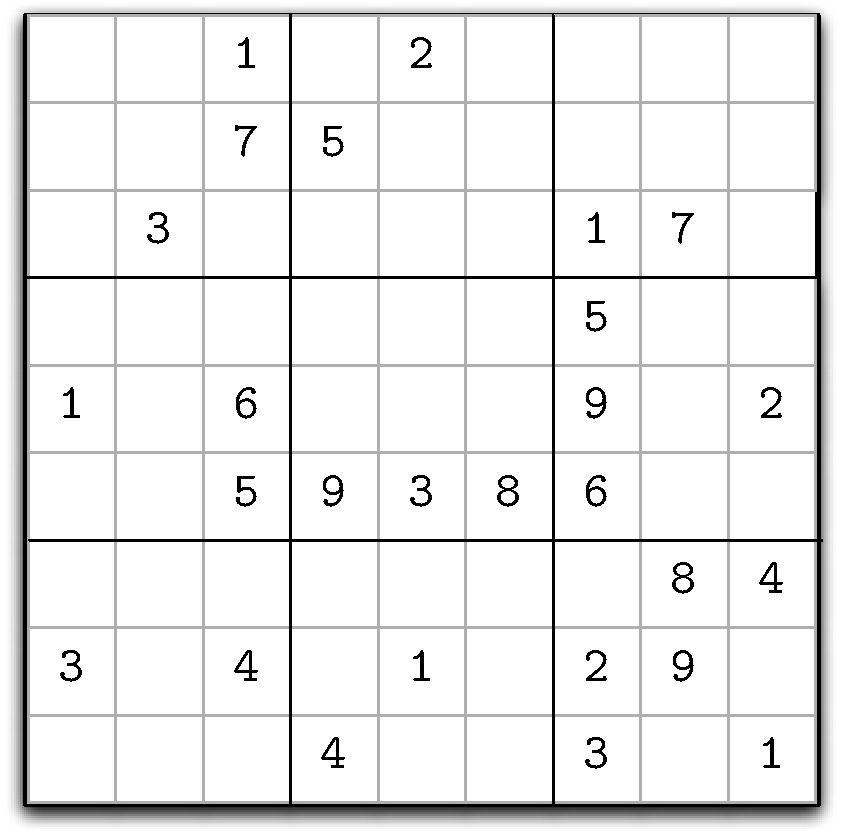
\includegraphics[width=2.5in]{unsolved}
%\end{boxed}
\caption{\label{su:unsolved}A typical sudoku puzzle}
\end{figure}

\noindent
The sudoku puzzle is an excellent opportunity to explore the capabilities of \go in problem solving and, in particular in constraint solving. As we shall see, our solution highlights a large number of \go's features; including the use of anonymous classes to achieve the effect of \q{let} in functional programming languages.

\section{Sudoku Strategy}
\label{su:strategy}
\index{Sudoku!strategy}

The key operation in solving a sudoku puzzle is the elimination of alternatives. We can represent the contents of a square as a set of alternative numbers to place there. At each step in the solution we will use the existing information to eliminate choices; until eventually, there are no choices in any of the squares and the puzzle is solved.

For example, the $6^{th}$ row in Figure~\vref{su:unsolved} has four blank spaces. Taking only the row itself into consideration, we can say that each of the blank squares can take on any of the numbers 1,2,4, or 7. That is because the other digits are already taken in that row. However, for a given cell, we must not only take into account the other cells in the same row, but we must also take into account the other cells in the same column and the other cells in the same $3\times{}3$ quadrant that the cell is in.

Taking these into account, the $6^{th}$ row can be represented as in Figure~\ref{su:sixth}.

\begin{figure}[h]
%\begin{boxed}
\centering
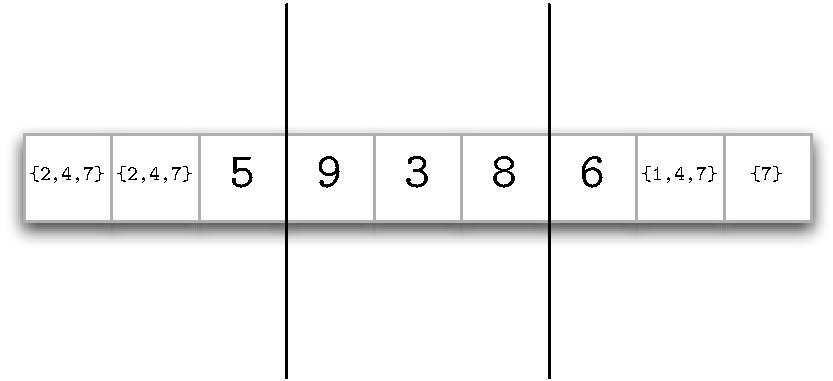
\includegraphics[width=2.5in]{sixth}
%\end{boxed}
\caption{\label{su:sixth}An annotated row}
\end{figure}

\subsection{Selecting a single solution}
Notice that the last square in the row has just one element in its set of possibilities -- namely 7. That means that we can infer that that cell has the number 7 in it.

Based on that choice, in the next step we can assign 7 to the last cell and eliminate 7 from the other cells -- giving the situation as in Figure~\vref{su:seven}.

\begin{figure}[h]
%\begin{boxed}
\centering
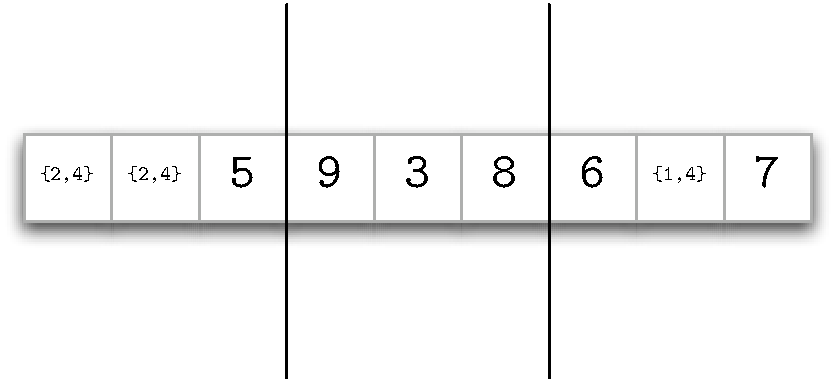
\includegraphics[width=2.5in]{seven}
%\end{boxed}
\caption{\label{su:seven}After selecting 7}
\end{figure}

\subsection{Unique elements}
In Figure~\vref{su:seven} we have reduced the possibilities to 2 or 4 in the first two cells and one of 1,2 or 4 in the $8^{th}$ cell. Notice that although this $8^{th}$ cell has three possibilities, it is the only cell in the row that the number $1$ appears in.

That means that we can infer that the $8^{th}$ cell must contain the number $1$ in it: even though currently there are three possibilities for that cell; the fact that we must be able to place all the digits and this is the only choice for $1$ allows us to assign $1$ to the $8^{th}$ cell. We show the resulting situation in Figure~\vref{su:one}.

\begin{figure}[h]
%\begin{boxed}
\centering
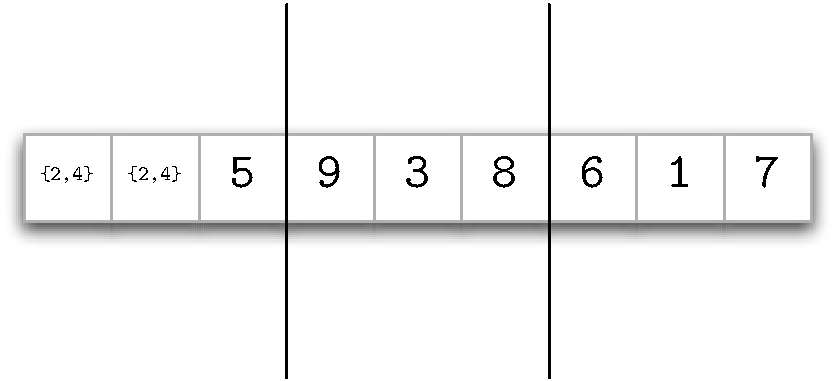
\includegraphics[width=2.5in]{one}
%\end{boxed}
\caption{\label{su:one}After assigning 1 to the $8^{th}$ cell}
\end{figure}
\noindent
After these steps we are left with both of the first two cells having the choice set \q{\{2,4\}}; and without further information we cannot infer any further constraints. However, solving the puzzle will involve iteratively looking at every row, column and quadrant in the same way.

\subsection{Cycling}
\label{su:cycle}
Thus a reasonable strategy for solving sudoku puzzles is the repeated application of three rules:
\begin{enumerate}
\item
Eliminate from cells' possible solutions any digit that has already be assigned to any cell in the same row, column or quadrant;
\item
If a cell's set of possibilities is reduced to one, then assign that number to the cell; and
\item
If a cell's set of possibilities contains a number that is not present in any of the other cells' possible sets in a given row, column or quadrant; then assign that number to the cell.
\end{enumerate}
\begin{aside}
It should never happen that a given cell's possible assignments contains \emph{more than one} choice which is not in any of the other cells' choices. That would be an unsolvable sudoku puzzle.

Again, if the set of choices for a cell is empty, then that puzzle also has no solution.
\end{aside}
Our program will solve sudoku puzzles by iteratively applying these rules to each row, column and quadrant until no further progress is possible.

By tradition, sudoku puzzles are deterministically solveable. However, a particularly fiendish puzzle setter may choose to \emph{under determine} the puzzle. In this case a puzzle solver is left with a set of constraints that cannot be further tightened by applying these rules and to solve the puzzle choices must be made.

Our program will steadfastly refuse to solve such puzzles and simply leave the puzzle in the partially solved state. It would, however, be relatively straight forward to extend the program to non-deterministically choose a partial solution and continue with the regular solving. If the solution attempt fails then a different choice would have to be made; until either solution is found or no solution is possible.

\section{Representing a sudoku puzzle}
The groundwork for our sudoku puzzler solver is the set of structures that we can use to represent the current state of the solver's problem. We do this with two key concepts: the structures needed to represent the choices in an individual cell in the square and the square as a collection of cells.

\subsection{Representing choices}
\label{su:choice}

At the heart of our sudoku solver is the notion of a set of possible choices for a given cell. Solving the puzzle involves progressive manipulation of this set of choices until only one choice remains -- the digit that must be assigned to that cell.

We can represent a set of choices as a \q{list[]} of \q{integer}s. However, we need to be able to manipulate this set, and so we shall \emph{encapsulate} the state of a cell in a stateful \q{constr} object.\note{A slightly more natural terminology would have been \q{cell}; however, that risks confusion with the standard \q{cell} package.}

We start our program by defining the type interface that defines the actions that we can perform on the set of choices of a cell:
\begin{alltt}
constr \impl \{
  curr:[]\funarrow{}list[integer].
  remove:[integer]*. assign:[integer]*.
\}.
\end{alltt}
There are three things that we can do with a cell's choices: find out what the \q{curr}ent set of choices is, we can \q{remove} a digit from the set, and we can \q{assign} a number to the cell.

It will also be convenient if we can have a consistent way of showing the contents of a cell's choices. However, since, all types inherit from the standard \q{thing} type, we do not need to explicitly call out the \q{show} type in the interface for \q{constr}.

Program~\vref{su:constr} shows an implementation of this type (sans any explicit \q{show} function. The current set of possible solutions is held in an object variable -- \q{L}; and this list represents the basis for reporting the \q{curr}ent set, q{remov}ing elements and so on.
\begin{program}
\vspace{0.5ex}
\begin{alltt}
constr:[list[integer]]\sconarrow{}constr.
constr(L0)..\{
  L:list[integer] := L0.

  curr()=>L.

  remove(K) ->
    L := L \bsl{} [K].

  assign(K) ->
    ( K in L ? 
      L := [K]).
\}.
\end{alltt}
\vspace{-2ex}
\caption{Recording choices in a cell}
\label{su:constr}
\end{program}
The \q{remove} program uses an operator that we have not yet encountered in our exploration of \go: the \q{\bsl{}} set subtraction operator. This, together with other set operations is defined in a standard \go package: \q{go.setlib}. The \q{\bsl{}} operator is special in that it is a standard operator of the \go language, but its implementation is strictly conventional:\note{This is an illustrative implementation of the set subtraction operator.}
\begin{alltt}
L\bsl{}M => \{ e .. (e::\nasf{}e in M) in L \}
\end{alltt}

The \q{go.setlib} package offers a set-like layer on top of ordinary \go lists -- by providing operators that preserve the setness property. I.e., if \q{L} and \q{M} are set-like lists (with no duplicate entries), then the result of subtracting \q{M} from \q{L} will also be set-like. The other set operators supported by \q{go.setlib} are set union (\q{\union}) and set intersection (\q{\intersection}).

Program~\ref{su:constr}'s function is really to \emph{record} the result of applying constraints to the cell -- the constraints arising from sudoku itself do not appear here.

\subsection{A Sudoku Square}
\label{su:table}
\index{Suduko!representing the square}

The kinds of rules that we discussed in Section~\vref{su:cycle} imply that we need to process the complete sudoku square in a number of different ways: processing each row of the square, each column of the square and each quadrant of the square. Traditionally, laying out a matrix like this seems to imply a choice: whether to have the matrix in row-column form or in column-row form. A row-column layout favors column-oriented processing, and a column-row layout favors row-oriented processing. However, because we also need to be able to process the table both in row-orientation and in column orientation. Furthermore, we \emph{also} need to support quadrant-oriented processing. This will strongly affect how we represent the cells in the sudoku square.

Manipulating a square array in this way is not especially unique to Sudoku (although it is not all that often that one needs to process the quadrants of a matrix). In particular, we do \emph{not} need to tie it to the contents of each cell: we are accessing rows, columns, etc., but they could be row of anything. I.e. this suggests a polymorphic type interface to the \q{square} concept:
\begin{alltt}
square[t] \typearrow{} \{ 
  colOf:[integer]\funarrow{}list[t]. 
  rowOf:[integer]\funarrow{}list[t].
  quadOf:[integer]\funarrow{}list[t].
  cellOf:[integer,integer]\funarrow{}t.
  row:[integer]\{\}.
  col:[integer]\{\}.
  quad:[integer]\{\}.
\}.
\end{alltt}
For example, we shall use the \q{colOf} function to extract a column from the table -- as a vector represented as a list. Similarly the \q{quadOf} function will also return a particular vector from the table -- corresponding to the particular quadrant.

The \q{row}, \q{col} and \q{quad} predicates are defined over ranges of \q{integer}s which indicate the indices of the legal rows, columns and quadrants in the table. Note that we do not \emph{bake} into this interface the size of the square. In fact, we can have any size square that we want.
\begin{aside}
The size of a sudoku square has to be itself a perfect square. We can have a $4\times{}4$ sudoku square, a $16\times{}16$ sudoku square and so on; but a $5\times{}5$ square does not have quadrants that also have 5 elements in them.
\end{aside}
Program~\vref{su:square} shows the outer aspects of a class that implements the \q{square} interface.
\begin{program}
\vspace{0.5ex}
\begin{alltt}
square:[list[t]]\sconarrow{}square[t].
square(Init)..\{
  Els:list[t] = Init.
  Sz:integer = itrunc(sqrt(listlen(Init))).

  row(I) :- I in iota(1,Sz).
  col(I) :- I in iota(1,Sz).
  quad(I) :- I in iota(1,Sz).
  \ldots{}
\}.
\end{alltt}
\vspace{-2ex}
\caption{Top-level of a \q{square} class}
\label{su:square}
\end{program}
The \q{square} class constructor (it is a stateful constructor) takes as its argument a list of entries -- which is assumed to take the form of a linear list of all the entries in the square in row-order. The class has -- at this stage -- two internal object variables: the list of \q{Els} and the length of the square. For a $9\times{}9$ square, the list of entries should contain 81 elements and the variable \q{Sz} will be computed as $9$ from that list.

Note that since we cannot decide whether the square will be processed in primarily row-order or column-order (or quadrant order) we do not attempt to \emph{structure} the entries in any way: we simply leave it as a linear list. We will will do is access this list in ways that are consistent with the row-ordering or column-ordering. However, the elements of the list are effectively in row-ordering; as in Figure~\vref{su:elements}.
\begin{figure}[h]
%\begin{boxed}
\centering
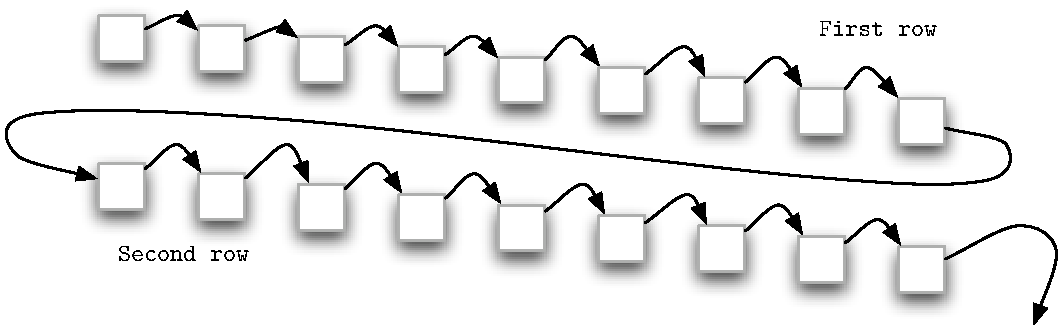
\includegraphics[width=3in]{elements}
%\end{boxed}
\caption{\label{su:elements}The elements in a \q{square} list}
\end{figure}
\noindent
It is arguable that a linear list is not an efficient way of representing the elements of a matrix. However, it is a simple technique and for our purposes efficient enough.

\subsubsection{Accessing a \q{row} out of the \q{square}}
The \q{square} interface allows us to extract the \emph{$n^{th}$} row as a separate list of elements. Since the list of elements is in row order, to access a given row we simply have to select the appropriate contiguous selection from the list of elements. To do this we use two functions that are part of \go's standard list-processing library: \q{drop} and \q{front}. 

The \q{front} function returns the first \emph{n} elements of a list, and \q{drop} is the converse: it returns the remaining elements after the $n^{th}$ element.
Program~\vref{su:rowof} shows how we can achieve this simply -- note that we are assuming that the first row, column and quadrant in the \q{square} is numbered from 1. The \q{rowOf} function is assumed to be textually within the class body for \q{square}.
\begin{program}
\vspace{0.5ex}
\begin{alltt}
rowOf(i) => front(drop(Els,(i-1)*Sz),Sz).
\end{alltt}
\vspace{-2ex}
\caption{Accessing a \q{rowOf} the square}
\label{su:rowof}
\end{program}

\subsubsection{Accessing a \q{col}umn out of the \q{square}}
Given that the list of elements in the \q{square} is in row order, accessing a column is slightly more complex: we have to access a cell from each row. 

The first cell in the column is at a position that depends on the number of the column. However, thereafter, successive elements of the column will always be a fixed distance away in the list -- the size of square governs this distance.

Program~\vref{su:colof}, which also should be viewed as being embedded in the \q{square} class body, shows how we can extract the elements that correspond to the column. We use an auxiliary function to access the subsequent elements from the list of \q{Els}. Note that \q{clOf} drops \q{Sz-1} elements from the list because that is the number of elements \emph{between} each element of a given column.
\begin{program}
\vspace{0.5ex}
\begin{alltt}
colOf(i) => clOf(drop(Els,(i-1)*Sz)).
  
clOf:[list[t]]=>list[t].
clOf([])=>[].
clOf([El,..L]) => [El,..clOf(drop(L,Sz-1))].
\end{alltt}
\vspace{-2ex}
\caption{Accessing a \q{colOf} the square}
\label{su:colof}
\end{program}
\noindent
The \q{clOf} recursion ends with the empty list; this works because \q{drop} will return an empty list if asked to drop more elements than are in the list. (This will be true after the last element of the column has been extracted.)

\subsubsection{Accessing a quadrant of the square}
Quadrants are a little like a combination of a row and a column: each row in the quadrant is contiguous within the list of elements, and successive rows in the quadrant are separated by a fixed number of other elements. Figure~\vref{su:quadrant} shows how the third quadrant is formed out of segments from the list.
\begin{figure}[h]
%\begin{boxed}
\centering
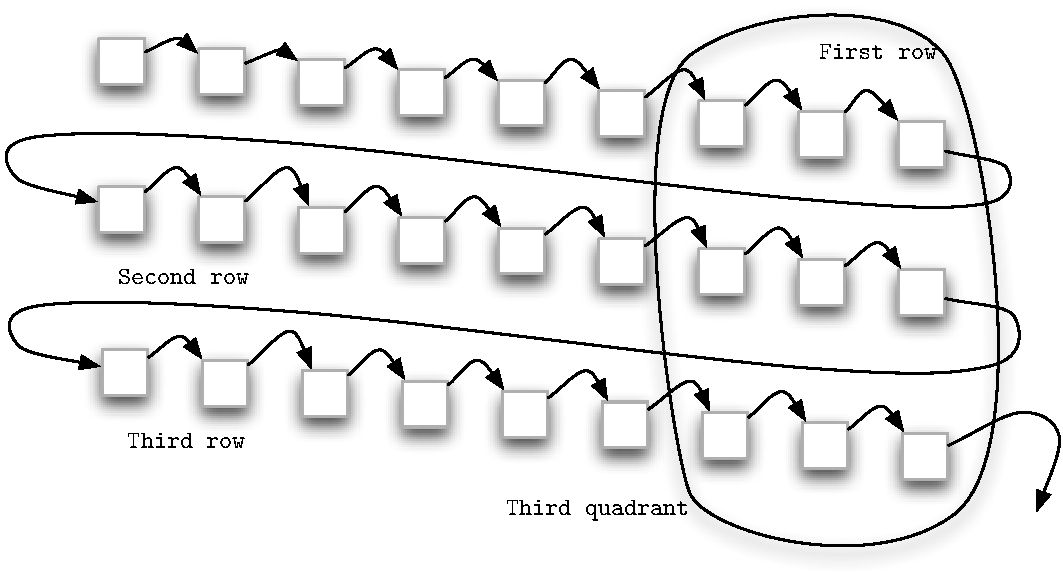
\includegraphics[width=3in]{quadrant}
%\end{boxed}
\caption{\label{su:quadrant}The elements in a quadrant}
\end{figure}
\noindent
Thus, once we have located the first row associated with the quadrant within the list of elements, extracting the rows of the quadrant is straightforward. We have to be a little more careful than when extracting the elements of a column as we will generally not be processing every row; and the gap between quadrant rows is less than the gap between entire rows.

Program~\vref{su:quad-1} shows how the successive elements of a quadrant are extracted.
\begin{program}
\vspace{0.5ex}
\begin{alltt}
Sq:integer = itrunc(sqrt(Sz)).

qdOf:[list[t],integer] => list[t].
qdOf(_,0)=>[].
qdOf(L,Cnt) => front(L,Sq)<>qdOf(drop(L,Sz),Cnt-1).
\end{alltt}
\vspace{-2ex}
\caption{Accessing the rows of a quadrant}
\label{su:quad-1}
\end{program}
\noindent
The \q{qdOf} function has two arguments: the list of elements to process and the number of segments to extract. The \q{Sq} object constant gives the length of each quadrant row (it is the square root of the length \q{Sz} of the square itself).

The tricksiest aspect of extracting a quadrant is deciding where to start extracting elements. If the size of the square is \q{Sz}, each row has $\sqrt{Sz}$ quadrants laid across it (a $9\times9$ square has three quadrants in each row, a $16\times16$ square will have 16 quadrants in total overlaying in a $4\times4$ grid over the square).

Similarly, there are $\sqrt{Sz}$ rows in a given quadrant. The total number of cells in a 'row of quadrants' is $\sqrt{Sz}\times{}Sz$ cells. For example, in a $9\times9$ square, each row of quadrants is 27 cells.

Thus the $i^{th}$ quadrant originates at cell
\[
((i-1)//\sqrt{Sz})\times\sqrt{Sz}\times{}Sz+(i-1)|\sqrt{Sz}
\]
where $A//B$ means the integer part of the quotient of $A/B$ and $A|B$ means the modulus of $A$ with respect to $B$. The computation with the integer quotient and modulus is required to select the quadrant's row of in the rows of quadrants.

For example, in a $16\times16$ square, the fifth quadrant (recall that that will be the first quadrant in the second row of quadrants) will be at cell 
\[
((5-1)//\sqrt{16})\times\sqrt{16}\times16+(5-1)|\sqrt{16} = 64
\]
We use this calculation in Program~\vref{su:quad-2} to initiate the extraction of the segments of the appropriate quadrant.
\begin{program}
\vspace{0.5ex}
\begin{alltt}
Sz2:integer = Sq*Sq*Sq.   -- compute Sz^1.5

\ldots{}
quadOf(i) => qdOf(drop(Els,
                     ((i-1) quot Sq)*S2+imod((i-1),Sq)*Sq),
                  Sq).
\end{alltt}
\vspace{-2ex}
\caption{Finding the right quadrant}
\label{su:quad-2}
\end{program}

\begin{aside}
After this, we leave the computation needed to access a single cell of the square to the reader!
\end{aside}

\section{Solving the Sudoku puzzle}
\label{su:solve}
\index{Sudoku!solving the puzzle}

The key to our algorithm is the repeated application of the rules that we identified in Section~\vref{su:cycle}. These are essentially the application of two kinds of filter, and the subsequent assignment of answers.

\subsection{Constraint filters}
\label{su:filter}

There are two kinds of filters that we need to apply: the elimination of impossible numbers from the sets of choices, and the identification of unique choices -- leading to the selection and subsequent elimination of the selection from other cells.

\subsubsection{Elimination filter}
The elimination filter has the very simple task of removing a specific number from the choices available to a given row, column or quadrant. Given the form of the \q{square} interface, we will be able to apply each filter in a uniform manner: to a list of choices represented as \q{constr} objects.

Program~\vref{su:elim} shows the elimination filter: it is given a list of \q{constr} objects and a number to eliminate; and it eliminates it. The only issue is to make sure that if a \q{constr} contains \emph{only} the number to elimnate then we \emph{do not} eliminate it from that \q{constr}. The reason is that we use such structures to represent the situation where a number has been assigned to the cell.
\begin{program}
\vspace{0.5ex}
\begin{alltt}
elim:[list[constr],integer]*.
elim(Set,K) ->
  (El in Set *>
    (K in El.curr(), El.curr()\bsl=[K]?
      \{\}
    | El.remove(K); done:=false
    )
  ).
\end{alltt}
\vspace{-2ex}
\caption{Elimination filter}
\label{su:elim}
\end{program}
\noindent
We perform one additional chore in the \q{elim} action procedure: we set a global variable \q{done} to \q{false} whenever we actually \q{remove} an element from a set of choices. We will use this later to govern the overall cycling of the sudoku solver. This is also the reason for the slightly long-winded test:
\begin{alltt}
K in El.curr(), El.curr()\bsl=[K]
\end{alltt}
We only want to set the \q{done} variable when we are actually progressing the solving of the puzzle.

We can use \q{elim} from Program~\vref{su:elim} to write the elimination filter for a complete set. Program~\vref{su:singleton} searches a set for a singleton element and, if it finds one, uses that to apply the \q{elim} filter to the other elements of the set.
\begin{program}
\vspace{0.5ex}
\begin{alltt}
singleton:[list[constr]]*.
singleton(Set) ->
  ( El in Set *>
    ( El.curr()=[K] ?  -- do we have a singleton?
      elim(Set,K)
    | \{\}
    )
  )
\end{alltt}
\vspace{-2ex}
\caption{Filtering for singletons}
\label{su:singleton}
\end{program}

\subsubsection{Uniqueness filter}
The complement case for singleton elements is where a given choice contains a number that does not appear in any other choice. In that case we can assign the cell that choice -- and subsequently the singleton filter will remove that choice from the other elements of the set.

Finding a unique element of a set of choices means finding an element that does not occur elsewhere. The \q{unique} predicate defined in Program~\vref{su:unique} is satisfied of a digit \q{U} if there is a nontrivial element in the set of choices that has \q{U} in it, and that \q{U} does not appear elsewhere in the set.
\begin{program}
\vspace{0.5ex}
\begin{alltt}
unique:[list[constr],constr,integer]\{\}.
unique(Set,Ot,U) :-
  append(F,[Ot,..B],Set),
  Cn = Ot.curr(), nontrivial(Cn),
  U in Cn, 
  \nasf(E in F, U in E.curr()),
  \nasf(E in B, U in E.curr()). 
\end{alltt}
\vspace{-2ex}
\caption{Finding unique choices}
\label{su:unique}
\end{program}
Program~\vref{su:unique} is formulated slightly differently to the \q{singleton} filter in Program~\vref{su:singleton}: we are using a call to the standard predicate \q{append} to non-deterministically \emph{partition} the set into three  pieces: a front piece (we call \q{F}), a back piece (we call \q{B}) and the element in the middle. The query
\begin{alltt}
append(F,[El,..B],Set)
\end{alltt}
accomplishes all of that. 

The two query conditions of the form
\begin{alltt}
\nasf(E in F, U in E.curr())
\end{alltt}
and
\begin{alltt}
\nasf(E in B, U in E.curr())
\end{alltt}
verify that the selected \q{U} does not appear in the \q{F} and \q{B} pieces.

Note that if there is no suitable candidate then the \q{unique} filter will \emph{fail}; a fact that we make use of in Program~\vref{su:uniqueset} which applies the \q{unique} filter where possible.
\begin{program}
\vspace{0.5ex}
\begin{alltt}
findUnique:[list[constr]]*.
findUnique(Set) ->
  ( unique(Set,Ot,U) *>
	 Ot.assign(U); done:=false
  ).
\end{alltt}
\vspace{-2ex}
\caption{Filtering for unique choices}
\label{su:uniqueset}
\end{program}
Note that, here also, we set the global \q{done} variable to \q{false} when we actually make a change to the choices in the set.

\subsection{A filter cycle}
The filters that we established in Section~\vref{su:filter} need to be applied to each row, column and quadrant in the square. This will involve iterating over those rows, columns and quadrants. This, in turn, builds on the \q{rowOf}, \q{colOf} and \q{quadOf} functions that we defined in Section~\vref{su:table}.

Program~\vref{su:applyall} shows one straightforward way of tackling this iteration: we define an auxiliary procedure \q{filterSet} that applies all the filters to a given row, column or quadrant. A complete cycle involves applying \q{filterSet} to each possible row, column and quadrant.
\begin{program}
\vspace{0.5ex}
\begin{alltt}
filterSet:[list[constr]]*.
filterSet(Set) ->
	singleton(Set);
	findUnique(Set).

applyAll:[square[constr]]*
applyAll(Square) ->
  ( Square.rowOf(R) *> filterSet(R));
  ( Square.colOf(R) *> filterSet(R));
  ( Square.quadrantOf(R) *> filterSet(R)).
\end{alltt}
\vspace{-2ex}
\caption{Apply filters}
\label{su:applyall}
\end{program}

\subsubsection{Are we done yet?}
Our strategy for solving a sudoku puzzle is inherently iterative. When a filter reduces the set of choices, or makes a selection, we rely on that action resulting in the potential for more constraints to be applied. In this way, constraints \emph{propagate} throughout the problem space until no more constraints trigger.

Only when no constraint can be applied can we ask whether we have solved the puzzle or not: if, when no further filters apply, there are only singleton sets in the square, then we know that we have solved the puzzle.

Recall that in the filter programs we set a global variable whenever we actually applied one of the filters. We will now use this global variable to control the cycles. In fact, \q{done} is not a truly global variable, we will put it -- together with the filter programs -- inside an \emph{anonymous} class; used as a kind of \q{let} expression.

\go does not directly have the kind of \q{let} expression that one encounters in functional programming languages. However, it is not needed either. First of all, let us define a somewhat simple type interface that will allow us to \q{do} things:
\begin{alltt}
do \impl \{ do:[]* \}
\end{alltt}
If we had a class that implemented this type, it may look like:
\begin{alltt}
do:[]\sconarrow{}do.
do..\{
  done:logical := false.
  
  do()::done -> \{\}.
  do() ->
    done := true;
    \ldots     -- possibly reset done
    do().
\}
\end{alltt}
This form is a pattern that can be used to govern a certain kind of iteration where the condition that governs the loop is not easily centralized (as in our case).

We have seen a number of examples of \go classes where the definition is essentially statically defined at the top-level of the package. However, \go supports classes in other contexts as well: classes can be defined \emph{inside} other classes -- i.e., inner classes (see Section~\vref{lo:inner}). In fact, classes can be defined \emph{in-line}: an \emph{anonymous} class
\index{anonymous class}
is simultaneously a class definition, and an occurrence of its constructor. We can use this to achieve the equivalent of \q{let} expressions. Program~\vref{su:cycleall} shows how we create an anonymous instance of the \q{do} type, and invoke its \q{do} action method to iterate our puzzle solver.

\begin{program}
\vspace{0.5ex}
\begin{alltt}
  solve:[square[constr]]*.
  solve(S) ->
    (:do..\{
      done:logical:=false.
      
      do()::done -> \{\}.
      do() ->
        done:=true;
        applyAll(S);
        do().
        
      \ldots
      applyAll:[square[constr]]*
      \ldots
    \}).do().
\end{alltt}
\vspace{-2ex}
\caption{Solving the sudoku}
\label{su:cycleall}
\end{program}
The construction:
\begin{alltt}
:do..\{ \ldots \}
\end{alltt}
is the anonymous class being defined. Like all programs, it must be declared and the type of this anonymous class is \q{do}. 

An anonymous class is called anonymous because there is no real name for the class; because it is simultaneously a class definition and a constructor for the class, the only handle is the object value of the anonymous class expression.

Our \q{solve} action procedure in Program~\vref{su:cycleall} creates the anonymous instance and invokes its \q{do} action method.

Note that the variable \q{S} is not passed explicitly into \q{do} -- it is a \emph{free variable} of the anonymous class. \go arranges that the correct value is supplied to the \q{applyAll} action call. Similarly, the \q{done} variable is free in the various filter programs -- all of which must be textually located within the \q{do} anonymous class otherwise the variable \q{done} will not be accessible to them.

\subsection{Putting it all together}
We have now established all the major pieces of our sudoku solver. Our final task is to arrange for the solver to be given the puzzle to solve, and to display the solution. 

In a complete application we would construct the puzzle to solve by reading a description of the puzzle from the keyboard. However, for the sake of brevity we will not be doing that in this chapter. 

The complete \q{sudoku} solver, including some details omitted here, is shown in Section~\vref{sample:sudoku}


\addtocontents{lop}{\protect\addvspace{1ex}}

\part{\go in detail}
\label{inDetail}

\chapter{Types}
\label{types}

\go is a statically checked strongly typed language. 
Strong typing means that every variable and every expression has a single type associated with it, and that the uses of these expressions are consistent with expectations. Static type checking means simply that types are checked at compile-time rather than at run-time.  Type errors arise when type checking detects an inconsistency. For example, if a function \q{foo} is defined over lists, then passing a numeric valued expression to \q{foo} is inconsistent because no list is equal to any number. 

\section{\go's type language}
\index{type terms}
\index{semantics of types}
\go's type language is founded on four key concepts. The \firstterm{type expression}{A type expression is a term that \emph{denotes} a type. A simple type expression would be something like the symbol \q{char} -- which denotes the type of character expressions. A more complex example would be \q{list[char]} which denotes lists of characters -- i.e., strings.} is a term that denotes a type.

Type terms are related to each other by the \emph{sub-type} relation: which represents a partial ordering on type terms. The sub-type relation is indicated by the programmer explicitly declaring which type terms are sub-types of other type terms -- as part of type definition statements.

The third key concept is the \firstterm{type interface}{An interface is associated with a type that defines the legal operations on values of that type. More specifically, the interface defines the expressions possible on the right hand side of a `dot' expression.}. A type interface defines the set of queries and operations that may be performed relative to a labeled theory -- specifically, it defines the kinds of `dot' references that are supported by a given type of value. All named types, including system types, may support an interface. If the type term defines what kind of value an expression has, the type interface defines to a large extent what you can do with the value.

Every expression in a \go program is associated with a type term which is called the expression's \firstterm{type assignment}{A type assignment of an expression is a mapping from the expression to a type term.} or \emph{type denotation}.

In addition to the type assignment, there are a number of \firstterm{type constraints}{a type constraint is a predicate that must be satisfied if the program is to be \emph{type safe}.}. Type constraints encode the rules for type safety in programs. There are two kinds of type constraints, type \emph{inequality} constraints that reflect the sub-type relationship and \emph{program} constraints that reflect the program being type checked.
Typically, program constraints are constraints on the arguments of functions and other programs; for example, that the type of a function argument is the declared argument type, or a sub-type of the declared type. A program is \emph{type safe} if there is a single consistent type assignment for all the identifiers in the program and the set of all the inferred type predicates are consistent.

\subsection{Sub-type constraint}
\label{type:subtype}
A sub-type constraint is a statement of the form:
\begin{alltt}
T \impl Tp
\end{alltt}
where \q{T} is a named type and \q{Tp} is a named type or a type interface. This statement declares that \q{T} is a sub-type of \q{Tp}. For example, the statements:
\begin{alltt}
student \impl person.
marriedStudent \impl student.
\end{alltt}
declare that \q{student} is a sub-type of \q{person}, and that \q{marriedStudent} is a sub-type of \q{student} and hence of \q{person}. So the constraint:
\begin{alltt}
T \impl person
\end{alltt}
is satisfied if \q{T} is \q{person}, \q{student} or \q{marriedStudent} -- or some other sub-type of the \q{person} type.

In the case that \q{Tp} is an interface, as in, for example,
\begin{alltt}
person \impl \{ age:[]=>integer\}
\end{alltt}
then this means that the \q{person} type implements an interface that includes an \q{integer}-valued function \q{age}.

We can combine, for a given type, the two forms of type statement:
\begin{alltt}
student \impl \{ studies:[]=>string\}.
student \impl person.
\end{alltt}
This means that \q{student} is a sub-type of \q{person} and that it also implements an interface with a \q{studies} function, the different interfaces are combined. Given only these two type statements, \q{student}'s full interface would be
\begin{alltt}
\{ studies:[]=>string. age:[]=>integer\}.
\end{alltt}

\subsubsection{A lattice of types}
The set of types forms a \firstterm{type lattice}{a partial ordering with an identified \q{top} element that is bigger than all others, and a bottom element \q{void} that is smaller than all other elements.}. A lattice is simply a set with a partial ordering associated with it; together with a top element (\q{top} in \go's case) which is larger than all other values and a bottom element (\q{void}) which is smaller than all others. A type lattice, as in figure~\vref{type:lattice}, is a kind of lattice where the elements are type terms; and the partial ordering is, in fact, the \emph{sub-type} relation. 

\begin{figure}
\centerline{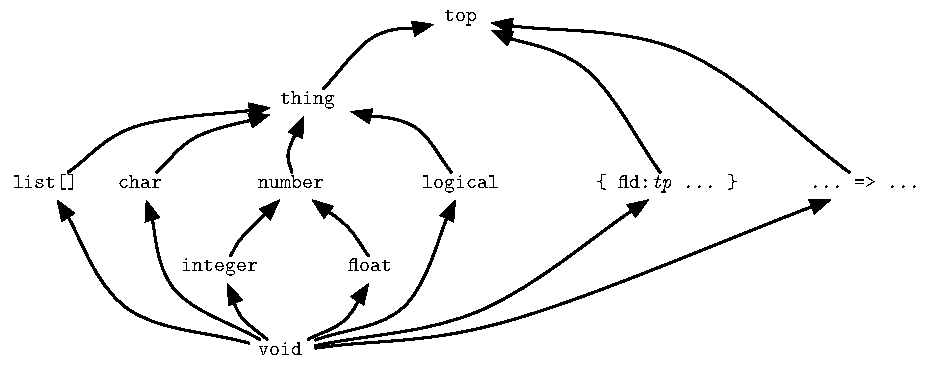
\includegraphics[width=\textwidth]{lattice}}
\caption{\label{type:lattice}Part of \go's standard type lattice}
\end{figure}

In the sub-type partial ordering, higher in the order means more general and lower in the ordering means more specific. Thus \q{top} type is the most general type (and therefore the least is known about values of type \q{top}) and \q{void} is so specific that there are \emph{no} legal \q{void} values.

The significance of \q{top} and \q{void} is largely technical, however, a function that accepts \q{top} arguments will accept anything and a \q{void} value is acceptable for all functions. On the whole, if you see either \q{top} or \q{void} in a type expression in an error message, you are likely to be in trouble!

You will notice that \go's type lattice is wide and shallow -- that for the most part there are few significant \firstterm{chain}{A chain is a sequence of types where for each pair of types in the link \emph{T\subi} and \emph{T\sub{i+1}} it  known that \emph{T\subi} is a subtype of \emph{T\sub{i+1}}. All types are in a chain of at least three elements: \q{void}, the type itself and \q{top}.}s in the lattice. This is in the nature of type lattice systems. However, when defining types, particularly in terms of type inheritance, then we do get a richer network. For example, figure~\vref{type:lattice:number} shows the lattice associated with the \q{number} type.

\begin{figure}
\centerline{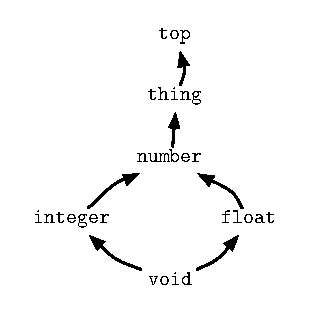
\includegraphics{numberlattice}}
\caption{\label{type:lattice:number}\go's \q{number} type lattice}
\end{figure}

This graph highlights the fact that a lattice is not necessarily a simple \firstterm{basket}{A basket type lattice is one where every chain is exactly three elements long; effectively meaning that there is no significant subtype relationship between non-trivial type elements.} or \emph{chain}, but can have have branching elements in it. It cannot, however, have cycles -- a lattice with a cycle is not permitted.

\subsection{Polymorphism}
Types  may be \firstterm{polymorphic}{A type that is not completely ground -- it may refer to many kinds of values.} and \firstterm{recursive}{A recursive type is one which may have components of the same type as the overall type.}. This polymorphism is reflected in the names of types -- they can have type arguments. For example, the \q{char} type is the type of characters; and \q{list[char]} represents the type list  of \q{char}acters -- i.e., \q{string}s.

The list type (\q{list[\emph{type}]}) is polymorphic: it requires a type argument which is the type of the elements of the list. It is also recursive because the type of a component element of a list term -- namely the tail of the list -- is also of the same type as the whole list.  A recursive type is one whose values contain components that are of the same type as the whole. Although the \q{list[\ldots]} type is built-in to \go, it is straightforward to define new recursive types. 

Recursive types have a particular hallmark: their type terms are \emph{opaque} -- it is not possible to infer solely from the type expression what values of that type look like. For example, although a list is necessarily defined as a term which includes a list as a component (the tail of a list is also a list of the same type) that recursion is not itself reflected in the \q{list} type term. In contrast with this, type expressions for functions are \emph{transparent} -- it is obvious from the type term what the structure of the values are -- and conversely, transparent types may not be recursive. For tuples, that means, for example, that it is not possible to define a tuple type in \go that has the same tuple type as itself as one of the elements of the tuple:
\begin{example}
\begin{boxed}
\begin{alltt}
( number, ( number, ( number, \ldots)))
\end{alltt}
\end{boxed}
\caption{\label{recursive:tuple}an impossible recursive tuple type}
\end{example}

\section{Standard Types}
\label{types:types}
\index{types}
\go has a range of built-in `atomic' types:  \q{integer}, \q{float}, \q{char} and \q{symbol}; and a range of built-in \emph{type constructors}:
\begin{itemize}
\item
\q{list[\emph{type}]} (list of \emph{type}), 
\item
\q{[\emph{type\sub1},\ldots,\emph{type\subn}]\{\}} (predicate type), 
\item
\q{[\emph{type\sub1},\ldots,\emph{type\subn}]=>}\emph{type} (function type), 
\item
\q{[\emph{type\sub1},\ldots,\emph{type\subn}]-->}\emph{type} (grammar type),
\item
\q{[\emph{type\sub1},\ldots,\emph{type\subn}]*} (action type), and
\item
\q{\{ \emph{field\sub1}:\emph{type\sub1}. \ldots \emph{field\subn}:\emph{type\subn}. \}} (type interface)
\end{itemize}

\subsection{Type variables}
\label{types:standard:variable}

\index{type variable}
\go does not use any special lexical markers to distinguish type variables from other variables, or even other type names -- the scope of the identifier serves to distinguish the cases. An identifier \q{foo} occurring in a type expression will refer to a type name if a type definition for \q{foo} is `in scope'; otherwise it refers to a type variable.

The normal scope rules do not apply for certain of \go's built-in types; for example, the identifier \q{number} (say) is predefined in the language and always refers to the \q{number} type.

\paragraph{Universally quantified types}
\index{unversally qunatified types}
\index{type variable!universal}
A \emph{universally} quantified type is written using the notation:
\begin{alltt}
[s\sub1,\ldots,s\subn]-\emph{Type}
\end{alltt}
this type binds the type variables s\subi{} occurring in the \emph{Type} expression. \go supports nested quantification of type terms: if \emph{Type} contains a type expression that is itself quantified and binds any or all of the \q{s\subi} type variables then the inner occurrences refer to the inner-most quantification.

It is not normally required to manually identify the type variables in a type expression in this way; however, when type expressions are printed (in error messages typically) they will be displayed in fully quantified form.


\subsection{Standard value types}
\label{types:standard}
\index{types!standard types}

Most of \go's standard types are defined in a standard library: \q{go.stdlib}. This library, which also includes a number of utility definitions, is automatically \q{import}ed in every package.\footnote{It is possible, if not advised, to suppress this behavior with a special compiler option.}

\subsubsection{\q{thing} type}
\label{types:standard:thing}

\index{thing@\q{thing} type}
\index{type!thing@\q{thing} type}

The \q{thing} type is the top of the value part of the type lattice -- all values are a sub-type of \q{thing}. It is not the top of the type lattice itself -- that is \q{top}. The program types -- such as function type -- are not a sub-type of \q{thing} -- although they are sub-types of \q{top}.

The \q{thing} type has a simple type interface; it is declared to be:
\begin{alltt}
thing \impl \{ 
  show:[]=>string.
  meta:[]=>meta.
  \}.
\end{alltt}
The \q{show} function is used to compute a printable \q{string} display of a term and \q{meta} is used to compute a meta-term representation of a term. Note that different types of terms may well use different methods for displaying themselves; it is only the \emph{type} of \q{show} that is defined at this juncture.
  

\subsubsection{\q{number} type}\
\label{types:standard:number}

\index{number@\q{number} type}
\index{type! number@\q{number} type}
The \q{number} type symbol is used to denote the union type of integer and floating point values and expressions. The \q{number} type has the definition:
\begin{alltt}
number \impl thing.
\end{alltt}

\subsubsection{\q{integer} type}
\label{types:standard:integer}

\index{integer@\q{integer} type}
\index{type!integer@\q{integer} type}
The \q{integer} type symbol is used to denote the type of integer values and expressions. The \q{integer} type has the definition:
\begin{alltt}
integer \impl number.
\end{alltt}

\subsubsection{\q{float} type}
\label{types:standard:float}

\index{float@\q{float} type}
\index{type! float@\q{float} type}
The \q{float} type symbol is used to denote the type of floating point values and expressions. The \q{float} type has the definition:
\begin{alltt}
float \impl number.
\end{alltt}

\begin{aside}
  Note that there is no subtype relationship between \q{integer}s and \q{float}s. They are, however, both subtypes of the standard type \q{number}.  This can occasional quirks where it is necessary to specifically convert \q{integer} values to \q{float}s using the built-in function \q{n2float}.
\end{aside}

\subsubsection{\q{char} type}
\label{types:standard:char}

\index{char@\q{char} type}
\index{type!char@\q{char} type}
The \q{char} type symbol is used to denote character values and expressions. The \q{char} type has the definition:
\begin{alltt}
char \impl thing.
\end{alltt}

\subsubsection{\q{symbol} type}
\label{types:standard:symbol}
\index{symbol@\q{symbol} type}
\index{type!symbol@\q{symbol} type}

The \q{symbol} type symbol is use to denote symbol values and expressions. Note that this type refers to the `general' class of symbols -- literals of which are written as identifiers surrounded by single quote characters. The other main class of symbols -- those introduced within user-defined type definitions are not covered by this type symbol; and nor are they written with single quotes.

The \q{symbol} type has the definition:
\begin{alltt}
symbol \impl thing.
\end{alltt}


\subsubsection{\q{logical} type}
\label{types:standard:logical}
\index{logical@\q{logical} type}
\index{type!logical@\q{logical} type}

The \q{logical} type is used to denote truth values. Although a standard type, \q{logical} can be defined as a normal user-defined type, using the type definition:
\begin{alltt}
logical ::= true | false.
\end{alltt}

\subsubsection{\q{opaque} type}
\label{types:standard:opaque}
\index{opaque@\q{opaque} type}
\index{type!opaque@\q{opaque} type}
The \q{opaque} type symbol is used to denote certain `internal' values that are managed by the \go system. There is no written notation that corresponds to opaque literal values, and they will never be displayed in normal circumstances.

\subsubsection{\q{meta} type}
\label{types:standard:meta}
\index{meta@\q{meta} type}
\index{type!meta@\q{meta} type}

The \q{meta} type is used to represent a meta-level representation of a term. It is defined using the definition:
\begin{alltt}
meta \impl thing.
\end{alltt}

\subsubsection{Tuple type}
\label{types:standard:tuple}
\index{tuple@\q{,} type}
\index{type!tuple@\q{,} type}

The \q{,} type is used to denote pairs of values. Although a standard type, \q{,} can be defined as though it were a normal user-defined type, using the definition:
\begin{alltt}
(u,v) ::= (u,v).
\end{alltt}
This rather bizarre type definition declares that the tuple type -- denoted by the type term \q{(u,v)} has a single constructor, also \q{(u,v)}. This notation is a slight twist on the normal type notation -- we are using the \q{,} operator as an infix type operator which is not actually permitted in programs.

\subsubsection{\q{list} type}
\label{types:standard:list}

The list type is used to denote lists of values. The list type is written using the notation:
\begin{alltt}
list[\emph{type}]
\end{alltt}
For example, the type expression:
\begin{alltt}
list[char]
\end{alltt}
denotes the type `list of \q{char}'. This is the type assignment given to expressions which are inferred to be lists of \q{char}acter -- including string literals. \go supports the \q{string} synonym for the \q{list[char]} type term.

The \q{list} type has a definition equivalent to:
\begin{alltt}
list[t] \impl thing.
list[t] \impl \{
    head:[]=>t.                -- head of the list
    tail:[]=>list[t].          -- tail of the list
    eof:[]\{\}.                  -- is the list empty
    cons:[t]=>list[t].         -- new list on the front
    tack:[t]=>list[t].         -- new list on the back
    hdtl:[t,list[t]]\{\}.        -- pick off the head and tail
    eq:[list[t]]\{\}.            -- is equal to this list
\}
\end{alltt}

\subsection{Program types}

\subsubsection{Type modes}
\index{type mode}

Program types have argument types that denote the types of arguments to the program. However, the types of arguments are also associated with \emph{modes} -- which express constraints on the flow of information into or out of a program via its arguments.

There are four kinds of modes: input mode, super-input mode, output mode and bidirectional mode:
\begin{description}
\item[input mode]
If an argument is marked as being input mode then the expectation is that data flows into the program through that argument. This carries two implications: one for type checking and one dynamic data flow:
\begin{itemize}
\item
An actual argument to a program that corresponds to an input moded argument may have a type that is a sub-type of the expected type.
\item
An actual argument to a program must not be \emph{bound} as a result of the matching of input arguments to patterns. Where the actual argument is a non-variable, this is not an issue; where the actual argument is an unbound variable then either the matching pattern also corresponds to an unbound variable or the match will \emph{fail}.
\item
In order to explicitly note an argument type to be input, suffix the type of the argument with the \q{+} operator:
\begin{alltt}
pp:[integer+]\{\}
\end{alltt}
\end{itemize}

\item[super input mode]
The super input mode is based on the input mode; with the additional operational characteristic that if a program is invoked where the super input moded argument is unbound then the call to the program is \emph{delayed} until such time as the variable becomes bound.

If the variable is never instantiated, then the delayed program is never invoked.

The super input mode is marked by suffixing the type of the argument with the \q{++} operator:
\begin{alltt}
listOfInt:[list[integer]++]\{\}
\end{alltt}

\item[output mode]
An output moded argument is the converse of an input moded argument:
\begin{itemize}
\item An actual argument's type must be \emph{equal} to the expected type for that program argument.
\item at run-time an actual argument \emph{must} be an unbound variable; otherwise the matching of patterns to values will \emph{fail} even if the corresponding pattern is an unbound variable.
\item
In order to explicitly note an argument type to be output, suffix the type of the argument with the \q{-} operator:
\begin{alltt}
pp:[integer-]\{\}
\end{alltt}
\end{itemize}

\item[bidirectional mode]
A bidirectional moded argument can be either input or output; and unification is used to match the actual argument to the pattern.
\begin{itemize}
\item
The type of the actual argument must be equal to the expected type for that argument
\item
Unification is used to match the incoming value against the pattern; hence the flow of information may be either incoming, outgoing or a mixture.
\item
In order to explicitly note an argument type to be bidirectional, suffix the type of the argument with the \q{-+} operator:
\begin{alltt}
pp:[integer-+]\{\}
\end{alltt}
\end{itemize}
\end{description}

Although it is possible to associate modes with every argument type of every program type, program types have defaults that are intended to represent the normal mode of use for that kind of program.

\subsubsection{Function type}
\label{types:standard:function}

The function type is used to denote function values. The function type is written:
\begin{alltt}
[\emph{T\sub{1}},\ldots,\emph{T\sub{n}}] \funarrow{} \emph{T\sub{R}}
\end{alltt}
where \q{[\emph{T\sub{1}},\ldots,\emph{T\sub{n}}]} is a list of the type expressions corresponding to the arguments of the function and \emph{T\sub{R}} corresponds to the result of the function. For example, the type expression:
\begin{alltt}
[list[char],list[char]]=>list[char]
\end{alltt}
denotes a function -- from two string arguments to a string result.

The default mode for function arguments is \emph{input}. However, it is occasionally useful to mark a function argument as output -- as an out-of-band way of returning values from a function.

\subsubsection{Predicate type}
\label{types:standard:predicate}

The predicate type is used to denote relational or predicate values. The predicate type is written:
\begin{alltt}
[\emph{T\sub{1}},\ldots,\emph{T\sub{n}}]\{\}
\end{alltt}
where \q{[\emph{T\sub{1}},\ldots,\emph{T\sub{n}}]} is the list of type expressions of the arguments of the predicate. For example, the type expression:
\begin{alltt}
[list[char],list[char],list[char]]\{\}
\end{alltt}
denotes the type of a ternary predicate where all the arguments are strings.

The default mode for predicate arguments is \emph{bidirectional}. However, it is often useful to mark a predicate argument as input -- to be explicit about the expect usage of the predicate.


\subsubsection{Action type}
\label{types:standard:action}

The action type is used to denote procedure values. The action type is written using a postfix \q{*} operator:
\begin{alltt}
[\emph{T\sub{1}},\ldots,\emph{T\sub{n}}]*
\end{alltt}
where \q{[\emph{T\sub{1}},\ldots,\emph{T\sub{n}}]} is the list of type expressions of the arguments of the procedure. For example, the type expression:
\begin{alltt}
[list[char]]*
\end{alltt}
denotes the type of a unary procedure whose single argument is a string.

The default mode for action procedure arguments is \emph{input}. However, it is occasionally useful to mark an argument as output -- as that is the only way of arranging for output from an action procedure call.

\subsubsection{Grammar type}
\label{types:standard:grammar}

The grammar type is used to denote grammar values. The grammar type is written as a \q{-->} mapping from the types of the arguments of the grammar to the type of the stream of values the grammar is defined over:
\begin{alltt}
[\emph{T\sub{1}},\ldots,\emph{T\sub{n}}] --> \emph{T\sub{S}}
\end{alltt}
where \q{[\emph{T\sub{1}},\ldots,\emph{T\sub{n}}]} is the list of type expressions of the arguments of the grammar and \emph{T\sub{S}} is the type of the stream that the grammar is defined over -- typically a list of some kind. For example, the type expression:
\begin{alltt}
[number]-->list[char]
\end{alltt}
denotes the type of a grammar whose single argument is a number and which may be used to parse strings.

The default mode for grammar arguments is \emph{bidirectional}. However, it is occasionally useful to mark a grammar argument as input -- to be explicit about the expect usage of the grammar, and also to mark an argument as output -- to be explicit about the outputs associated with parsing a stream.

\subsubsection{Class type}
\label{types:standard:class}

\index{type!class}
\index{class type}
\index{type!@= type operator}
There are two kinds of class type declarations: those that introduce a stateless class and those that introduce a stateful class.

The state-free class type is used to denote constructor classes, analogous to constructor functions. The stateful class type denotes classes that may carry state.


A state-free class type declaration takes the form:
\begin{alltt}
\emph{class}:[\emph{T\sub1},\ldots,\emph{T\subn}] @= \emph{Type}.
\end{alltt}
The only permitted mode for the label arguments of a state-free class label is \emph{bidrectional}.

A stateful class type declaration takes the form:
\begin{alltt}
\emph{class}:[\emph{T\sub1},\ldots,\emph{T\subn}] @> \emph{Type}.
\end{alltt}
The default mode for label arguments of a stateful class label is \emph{input}.

\begin{aside}
The reason that state-free label arguments must be bi-directional is that class labels are equivalent to constructor functions: i.e., they have an inverse. That means that it is always possible to recover the arguments of a 'call' to a constructor function.

On the other hand, one of the differences between state-free class labels and statefull class labels is that the latter \emph{do not} have inverses -- they are semantically closer to regular functions.
\end{aside}
Note that a class type statement does not define the class itself, it simply defines its type.

\section{Algebraic type definitions}
\label{type:algebraic}

In addition to a type being defined using the sub-type statements, a type may also be introduced using an \emph{algebraic type definition} statement. An algebraic type definition is one where the type is introduced at the same time as a set of enumerated symbols and constructors for the type:
\begin{alltt}
\emph{UserT}[\emph{T}\sub1,\dots,\emph{T}\subn] ::= \dots\ | \emph{S} | \dots.
\end{alltt}
where \emph{T\subi} are identifiers indicating type arguments and the right hand side is a series of enumerated symbols and constructor function templates.

For example, the \q{tree} type defined below may be used to denote tree values:

\begin{alltt}
tree[a] ::= empty | node(tree[a],a,tree[a]).
\end{alltt}
This statement defines a new type type constructor \q{tree} together with the enumerated symbols and constructor terms that make up values of the \q{tree} type.

\subsection{Type parameters of a type definition}
\label{type:parameter}

Where the template of a \emph{UserType} takes the form:
\begin{alltt}
\emph{UserType}[\emph{T}\sub1,\dots,\emph{T}\subn] \impl \ldots
\end{alltt}
the various arguments \emph{T\subi} are the \emph{type parameter}s of the type definition. They must all be identifiers and they are interpreted as type variables. Such a \emph{UserType} is implicitly universally quantified with respect to the type parameters (hence the polymorphism of the type).

\go imposes a restriction on type variables occurring in a type definition: all type variables appearing in the body of the type definition -- i.e., appearing in templates for the type constructors in class definitions -- must also appear in the type template expression itself.

\subsection{Enumerated symbol}
\label{type:user-symbol}
An \emph{enumerated} symbol is equivalent to a zero-arity label term. For example, the introduction of \q{empty} in the definition of \q{tree} above is equivalent to the class definition:
\begin{alltt}
empty:tree[a] .. \{\}.
\end{alltt}

The type analysis of a definition of an enumerated symbol may be captured via an `introduced' type inference rule:
\begin{equation*}
\forall \vec{V}.\left\{\frac{}
{\typeprd{E}{\q{S}}{\q{\emph{UserT}[\emph{T}\sub1,\dots,\emph{T}\subn]}}}\right\}
\end{equation*}
where $\vec{V}$ are all the type variables ocurring in the type definition and \q{S} is the newly introduced enumerated symbol.

Note that, in general, the type of a enumerated symbol can have type variables even when clearly the symbol itself has no variables. We can see this more clearly with the empty list case. \go's list notation is based on the \q{,..} constructor function and the \q{[]} enumerated symbol; which might be captured in the algebraic type definition:
\begin{alltt}
list[T] ::= [T,..list[T]] | []
\end{alltt}
The type of an occurrence of the empty list is, then, an expression of the form:
\begin{alltt}
list[T\sub{i}]
\end{alltt}
where \q{T\sub{i}} may or may not be known. The logic of this is that an empty list is always of a list of a specific type -- even if we cannot determine what that type is in given circumstances.

\subsection{Constructor functions}
\label{type:constructor}
\index{contructor function definition}
\index{functions!constructor}

Constructor functions (a.k.a. class labels) are analogous to functors in \prolog: they fulfill very similar roles. However, their semantics are quite distinct to normal \prolog terms since they always are associated with logical theories -- even when defined within an algebraice type definition.

\begin{aside}
  Constructor functions are so-named because they are functions: with the
  particular property that every expression involving the constructor function
  has an exact inverse. This property allows constructor functions to be used as
  patterns as well as in other expressions.
\end{aside}

The type assignment for constructor functions can be viewed as an additional type inference rule; where a type definition was of the form:
\begin{alltt}
\emph{Template} ::= \ldots | \emph{F}(\emph{T\sub1},\ldots,\emph{T\subn}) | \ldots
\end{alltt}
we introduce a new inference rule of the form:
\begin{equation}
\LeftLabel{$\forall \vec{V}$}
\AxiomC{\typeprd{{\emph{E}}}{A\sub1}{\emph{T\sub{1}}}}
\AxiomC{\ldots}
\AxiomC{\typeprd{{\emph{E}}}{A\subn}{\emph{T\sub{n}}}}
\TrinaryInfC{\typeprd{{\emph{E}}}{\q{\emph{F}(\emph{A\sub1},\ldots,\emph{A\subn})}}
{\q{\emph{Template}}}}
\DisplayProof
\end{equation}
where $\vec{V}$ are the type variables ocurring in the type definition.

\subsection{Type extension}
One of the key features of \go's type system is its extensibility. In particular, because types are distinct from classes, there is always the potential to introduce new constructors for a type -- including types that have been introduced using an algebraic type definition.

For example, given the \q{tree[]} type, we may decide that we need a new kind of node for a tree -- perhaps a binary tree node that does not include a label. We can do so simply by defining a class for it:
\begin{alltt}
bin:[tree[a],tree[a]]@=tree[a].
bin(L,R) .. \{ \ldots \}
\end{alltt}
The effect of this is as though the original type definition were:
\begin{alltt}
tree[a] ::= empty 
        | node(tree[a],a,tree[a])
        | bin(tree[a],tree[a]).
\end{alltt}
We can even introduce this class in a different package than the one in which \q{tree[]} itself is defined:
\begin{alltt}
foo\{
  import tree.
  bin:[tree[a],tree[a]]@=tree[a].
  bin(L,R) .. \{ \ldots \}
\}
\end{alltt}
  


\addtocontents{lop}{\protect\addvspace{1ex}}
\chapter{Functions and Expressions}
\label{expressions}

This chapter is about the functional programming aspect of \go. \go has a rich range of expressions, one of its distinguishing characteristics when compared to \prolog. Part of this comes from the fact that \go combines a functional programming notation, and part comes from \go's multi-paradigm style: so there are expressions that relate expressions to actions and predicates as well as regular evaluable forms.

\section{Functions}
\label{expression:functions}
\index{functions}
\index{equations}

Functions are defined using sequences of equations. For example, Program~\vref{function:append} shows how a list concatenation function may be written. Each equation is a \emph{rewrite} equation that shows how to rewrite terms of one form -- representing the function call -- to terms of another form -- representing the value.
\begin{program}
\begin{boxed}
\begin{alltt}
concat:[list[T],list[T]]=>list[T].
concat([],X) => X.
concat([E,..X],Y) => [E,.. concat(X,Y)].
\end{alltt}
\end{boxed}
\caption{\label{function:append}A list \q{concat}enation function}
\end{program}
The type declaration says that \q{concat} is polymorphic, mapping a pair of lists of any type of element \q{T} to a list of elements of the same type.

Functions may be defined either within a class body -- in which case they are specific to that class -- or at the outer level of a package -- in which case they are global to the package. In both cases all the equations for a given function must be grouped together.

The general form of an equation is:
\begin{alltt}
\emph{Fun}(\emph{Ptn\sub1},\ldots,\emph{Ptn\subn} :: \emph{Condition} => \emph{Exp}
\end{alltt}
The equations in a function are applied in a left-to-right order. There is no deep backtracking in function evaluation: once an equation has been found that matches then no other equations will be attempted. In the event that none of the equations match an error exception
\begin{alltt}
error(\ldots,'eFAIL')
\end{alltt}
will be raised.

\paragraph{Matching equations to arguments}
\label{expression:equation:matching}
\index{equation!argument matching}
\index{argument matching in equations}
Note that, by default, the head arguments of an equation are \emph{matched} against the tuple of arguments rather than \emph{unified}. The distinction is that matching is not permitted to side-effect its input -- in this case matching against the head of an equation \emph{will not} side-effect the arguments to the function call.
For example, given a function application:
\begin{alltt}
F(X,2)
\end{alltt}
then if \q{F} is defined by the equation:
\begin{alltt}
F('a',2) => 3
\end{alltt}
then the match will \emph{fail} (and raise an error if there are no alternatives equations for \q{F}) since the only way that it could succeed would be by binding \q{X} to \q{'a'}. 

\begin{aside}
The only exceptions to this matching semantics are where the argument's mode as declared in the function's type declaration is bidirectional -- in which case the incoming argument will be \emph{unified} -- or if the argument is marked as output -- in which case the incoming argument must be an unbound variable and a value will be returned in that argument.

For example, the type declaration:
\begin{alltt}
F:[symbol-,integer]=>integer.
\end{alltt}
would require the above equation for \q{F} to be applied to a function call in which the first argument was unbound, and would permit equations that define \q{F} to instantiate the argument. 
\end{aside}

\begin{aside}
\index{match predicate}
\index{\q{.=} predicate}
The match predicate \q{.=} (see Section~\vref{goal:match}) may be used within a guarded term to achieve a similar matching semantics as for the head arguments themselves.
\end{aside}

The type inference rule for the equations defining a function \q{F} is:
\index{type inference!equation}
\begin{equation}
\AxiomC{\typeprd{\emph{E}}{\q{\emph{F}}}{\q{\emph{F\sub{H}}=>\emph{F\sub{R}}}}}
\AxiomC{{F\sub{H}}={T\sub{H}}}
\AxiomC{\subtype{F\sub{R}}{T\sub{R}}}
\TrinaryInfC{\typesafe{\emph{E'}}{\q{\emph{H}::\emph{G}=>\emph{R}}}}
\DisplayProof
\end{equation}
I.e., the main requirement for a safe equation is that the head arguments have the same types as the declared argument types and the type of the right hand side expression of the equation is less than or equal to the function result type.

\begin{aside}
Note that the type rule for an equation is independent of the modes associated with the function type. In all cases, the type of the argument pattern must be the same as the type of the function. Modes affect calls to functions, and hence the right hand sides of equations, but do not affect the type analysis of argument \emph{patterns}.
\end{aside}

\section{Atomic expressions}
\label{expression:atomic}

The atomic \go expressions are the atomic or unstructured elements of the language: including characters, symbols and numbers. They are called atomic because, from the \go programmer's perspective, they have no internal structure. 

\subsection{Symbols}
\label{expression:symbol}

\index{expression!symbols}
\index{symbol literal expression}
As outlined in Section~\vref{token:symbol}, a symbol is written as a sequence of characters enclosed in single quotes. Symbols are one of the primitive data types of \go, and have the type \type{symbol}.

We define the type inference rule for symbols thus:
\index{type inference!symbol}
\begin{equation}
\frac{}
{\typeprd{E}{\q{'\emph{S}'}}\q{symbol}}
\end{equation}
which is interpreted as
\begin{quote}
The type of an expression of the form \q{'\emph{S}'} is \q{symbol}.
\end{quote}

Logically, a symbol is a token that identifies an individual entity in the modeled world. \go supports other kinds of symbols than quoted \q{symbol}s; user defined symbols as introduced via class definitions or in algebraic type definitions do not carry the \q{symbol} type: their type is that of the declared type. Such symbols are written using the normal identifier notation.

\subsection{Characters}
\label{expression:character}

\index{expression!character}
\index{character expression}
A character literal is written as a back-tick character followed by the character itself; which may be a string character reference. Characters are one of the core data types of \go: lists of \q{char}acters form the basis of \go's string notation.

The type of a character expression is \q{char}:
\index{type inference!character}
\begin{equation}
\frac{}
{\typeprd{E}{\q{`\emph{C}}}\q{char}}
\end{equation}


\subsection{Numbers}
\label{expression:number}
%klc mostly copied from Lets Go!
\index{expression!number}
\index{number@\q{number} expression}
\go partitions numbers into two categories: \q{integer}s and \q{float}ing point numbers. Both of these are sub-types of the \q{number} type; however, neither \q{integer} nor \q{float} are sub-types of each other. This reflects the common reality that integral and non-integral \q{number} values are represented differently.

There are various ways of writing integer literals: as decimal integers, hexadecimal numbers and character codes.

\subsubsection{Integers}
\index{integer}
An integer is written as a sequence of decimal digit characters -- with an optional leading minus sign to denote negative integers. Although the standard ASCII digit characters are likely to be the most common digit characters used, there are approximately 250 decimal digit characters in the Unicode standard! The \go parser supports the use of any Unicode decimal digit characters in constructing a number; however, the \go system only uses ASCII digits when displaying numbers.

\paragraph{Hexadecimal numbers}
\index{integer!hexadecimal}
A hexadecimal number is written with a leading \q{0x} followed by hexadecimal digits. Note that, unlike regular integers, \go requires that hexadecimal numbers use only the ASCII digit characters, together with upper-case or lower-case letters \q{A} to \q{F}.

\begin{alltt}
0xffff 0xabd 0x0
\end{alltt}
are all integers, of type \q{integer}, written using hexadecimal notation.

\paragraph{Character codes}
\index{integer!character code}
\index{Unicode!character code}
It is also possible to specify an integer as the Unicode code value of a character. Such an \q{integer} is written with a leading \q{0c} followed by a single character reference. Thus, for example, the literal:
\begin{alltt}
0cA
\end{alltt}
is the number 65 -- as the Unicode code point value associated with upper-case \q{A} is 65. Similarly, \q{0c\bsl{}n} is the \q{integer} 10, as the character \q{\bsl{}n} refers to the new-line character -- whose code value is 10. The value of
\begin{alltt}
0c\bsl{}+2334;
\end{alltt}
is, of course, the same as:
\begin{alltt}
0x2334
\end{alltt}

\index{type inference!integer}
\begin{equation}
\frac{X \mbox{ is an integer literal}}
{\typeprd{E}{X}{\q{integer}}}
\end{equation}

\subsubsection{Floating point numbers}
\index{floating point}
\index{number!floating point}
\go distinguishes floating point numbers from integral values by the fact that floating point numbers always have a decimal point: i.e., a floating point number is written as a fractional number followed by a fractional part and an optional exponent expression. Example floating point numbers include:
\begin{alltt}
34.56 2.0e45 2.04E-99
\end{alltt}
Since the period character has so many uses in \go, there are some special rules for them. In the case of a floating point number there may be no spaces on either side of the period; i.e., the program text:
\begin{alltt}
34 . 23
\end{alltt}
does \emph{not} denote the number 34.23; it is three tokens: the integer 34, the rule terminator \q{\dotspace} and the integer 23.

Floating point literals are of type \q{float}, a sub-type of \q{number}.
\index{type inference!float}
\begin{equation}
\frac{X \mbox{ is a float literal}}
{\typeprd{E}{X}{\q{float}}}
\end{equation}

\section{Variables}
\label{expression:variable}

\index{expression!variable}
\index{variable expression}
Variables are written as identifiers (see Section \vref{token:identifier}). All identifiers which have not been defined as class labels or names of rule programs or declared as enumerated symbols or constructor functions in an algebraic type definition are considered to be variables. \go does not have a variable convention to distinguish variables; instead we use the context of the identifier to distinguish them. Note that normal symbols (see Section~\vref{expression:symbol}) are always surrounded by single quotes and cannot be confused with variables.

\index{type inference!variable}
All variables have types, and each occurrence of a variable is type-checked -- resulting in type constraints on its type: the constraints inferred with respect to each occurrence of a must be consistent.  

A variable may not have a value and yet still have a type associated with it.

\subsection{Scope of identifiers}
\label{variable:scope}

\index{variable!scope}
\index{identifier!scope}
\index{scope of identifiers}
\go does not require that variables in rules be explicitly introduced -- simply, an identifier occurring in a pattern or expression that does not have a prior declaration is assumed to be a variable. However, there are rules that define the \emph{scope} of a variable: i.e., the textual range across which occurrences of the same name are considered to refer to the same variable.

For identifiers such as program names, type names and class names, introduced in the body of a class or package, they are in scope across the entire class body or package -- there is no implied scope arising from the order of declarations. For variables in rules, the scope of the variable is the entire rule. Similarly, program names are in scope for their entire enclosing context, regardless of the order of declaration.

For a rule, such as an equation or a clause, any variables mentioned in the rule that are not defined in an outer scope -- either in an enclosing class body or as package variables -- are local to that rule.

A variable is \emph{free} in a rule if its scope encompasses the rule as well as other, enclosing, program fragments. The main source of free variables in a rule are \emph{label variables} of the class in which the rule is embedded. For example, in:
\begin{alltt}
lbl(X)..\{
  bar(X) :- X<10.
\}
\end{alltt}
the variable \q{X} is \emph{free} in the \q{bar} clause. The reason is that \q{X} is also a variable occurring in the label \q{lbl(X)} of the class that the \q{bar} clause is embedded.


\paragraph{Holes in the scope}
\index{variable!scope!holes in}
\index{identifier!scope!holes in}
A hole in the scope of an identifier  -- i.e., where an inner use of an identifier can `hide' an outer identifier with the same name -- can occur when the inner use of the identifier is as the name of a defined program of a class body.  The inner variable masks out, throughout its natural scope,  any variable of the same name defined in outer contexts. 

Note that variable identifiers in rules \emph{do not} mask out variables of the same name in outer scopes.  Such a variable is a \emph{free} variable of the rule. This is the principal mechanism in many cases whereby a program is referenced in function and predicate calls in the bodies of rules.

Consider the following definition of the state-free class:
\begin{alltt}
funny:[T\sub1,T\sub2,T\sub3] @= aType.
funny(A,Y,B)..\{
  A(X).
  A([X,..Y]) :- B.is(X),A(Y).
\};
\end{alltt}
The variable \q{B} introduced in the \q{funny} constructor is in scope across the whole of the class body defining \q{funny}. It is therefore a global variable of this class. 

The variable \q{A} is in scope throughout the class as well. However, there is a definition of \q{A} in the class body that uses the same name \q{A}; this definition masks out the \q{A} that occurs as a parameter of the \q{funny} constructor.  In effect, the \q{funny} class cannot use its \q{A} argument as it is masked by the inner \q{A} definition in the class body.

The \q{X} variable has two `incarnations': in the first clause of the definition of \q{A} and in the second clause. These are separate variables. The \q{X} of the first clause is local to that clause.

The \q{Y} variable occurring in the head of second clause of \q{A} is \emph{not} local -- it is bound by an outer occurrence of the same variable in the argument list of the \q{funny} constructor. Like the \q{B} variable in the same clause, it is a \emph{free} variable of the \q{A} program.

\paragraph{Singleton variables}
\index{variable!singleton occurrence}
Note that the compiler will report a warning over any \emph{singleton} occurrences of variables -- unless the variable has a leading underscore in its name. Such singleton variables are often actually misspelt variables -- hence the warning from the compiler. In this case, the compiler would report a warning over both the \q{A} parameter of the function and the \q{X} parameter of the first \q{A} clause. The former helping to highlight the fact that \q{A} is effectively masked out by the theta environment.

\subsubsection{Scope of type variables}
\index{scope!of type variables}
\index{type variables!scope of}
Like regular variables, type variables also have an associated textual scope. The scope rules for type variables are essentially the same as for normal identifiers. Of particular interest are type variables occurring within rules that are \emph{not} free -- i.e., are not mentioned in an outer context. Such type variables have the same scope as a regular variable: the rule in which the variable is mentioned.

\section{Standard structured terms}
\label{expression:structured}

\index{structured terms}
\go has two standard data constructor types: lists and tuples. In addition, of course, it is possible to define additional data constructors using class definitions and algebraic type definitions.

\begin{aside}
In fact, both lists and tuples are definable using normal \go mechanisms for defining constructor terms. They are highlighted because of their special role in the language.
\end{aside}

\subsection{Lists}
\label{expression:lists}

\index{list expression}
\index{expression!lists}
Lists are a standard data type of \go, the list data type is described in detail in Section~\vref{types:standard:list}. The surface syntax of lists is defined in Section~\vref{grammar:lists}. 

A list is a sequence of values. The defining characteristic of a list is that the first element of the list -- called  the \emph{head} of the list -- and the remaining sequence of elements after the head -- called the \emph{tail} of the list -- are available in a single constant step of computation. This distinguishes lists from arrays -- where every element is available in constant time although arrays are not easily extended -- and sets where each element may take $\log{}(n)$ time to access and there is only one occurrence of each element.

Lists are written as a sequence of comma-separated expressions enclosed in square brackets. For example, the list
\begin{alltt}
[1,2,3]
\end{alltt}
is a list of three \q{number}s: 1, 2 and 3, as is the expression:
\begin{alltt}
[1,1+1,1+1+1]
\end{alltt}

\paragraph{List pattern notation}
\index{lists!pattern}
There are two standard constructors for the list type: the empty list -- written as \q{[]} -- and the list cons constructor -- written as the special infix operator \q{,..} consisting of a head element and a tail list:
\begin{alltt}
[\emph{H},..\emph{T}]
\end{alltt}
There is a direct correspondence between list patterns and list terms: the expression:
\begin{alltt}
[1,[2,[3,..[]]]
\end{alltt}
is equivalent to the list \q{[1,2,3]}.

Other forms of list pattern are also interesting. For example, the list pattern:
\begin{alltt}
[1,2,3,..X]
\end{alltt}
denotes a list whose first three elements are known but whose tail is represented by the variable \q{X}. It is one of the magic aspects of logic programming that unifying \q{X} with \q{[4,5]} say, will have the effect of completing the above list pattern to
\begin{alltt}
[1,2,3,4,5]
\end{alltt}


The type rules for the standard list constructors are 
\index{type inference!lists}
\begin{equation}
\label{emptylist:type}
\AxiomC{}
\UnaryInfC{$\forall T.\typeprd{E}{\q{[]}}{\q{list[\emph{T}]}}$}
\DisplayProof
\end{equation}
and
\begin{equation}
\label{nonempty:type}
\AxiomC{\typeprd{E}{\q{H}}{T\sub{t}}}
\AxiomC{\typeprd{E}{\q{T}}{\q{list[{T\sub{t}}]}}}
\BinaryInfC{\typeprd{E}{\q{[H,..T]}}{\q{list[{T\sub{t}}]}}}
\DisplayProof
\end{equation}

\noindent
\index{type inference!complex expressions}
We can concatenate type inference rules to infer the types of more complex expressions. For example, we can use the type inference rules \ref{emptylist:type} and \ref{nonempty:type} to derive the type of this expression:
\begin{alltt}
[1,2]
\end{alltt}
which gives the type derivation:
\begin{prooftree}
\AxiomC{}
\UnaryInfC{\typeprd{E}{\q{1}}{\q{number}}}
\AxiomC{\typeprd{E}{\q{2}}{\q{number}}}
\AxiomC{\typeprd{E}{\q{[]}}{\q{list[T]}}}
\BinaryInfC{\typeprd{E}{\q{[2]}}{\q{list[number]}}}
\BinaryInfC{\typeprd{E}{\q{[1,2]}}{\q{list[number]}}}
\end{prooftree}



\subsection{Strings}
\label{expression:string}
\index{expression!strings}
\index{strings!lists of characters}
\index{lists of characters are strings}
\go string literal values are synonyms for lists of \q{char}s; i.e., a string literal such as \q{"foo"} is equivalent to the list:
\begin{alltt}
[`f,`o,`o]
\end{alltt}
and the empty string \q{""} is equivalent to
\begin{alltt}
[]:list[char]
\end{alltt}
i.e., an empty list with the added type annotation that it's type is list of \q{char}s (see Section~\vref{expression:typeannotation}).

\subsection{Tuples}
\label{expression:tuples}

\index{expression!tuple}
\index{tuple epxressions}
Like lists, tuples represent a way of aggregating values in a sequence. A tuple is written as a sequence of elements, separated by \q{,} and enclosed in parentheses:
\begin{alltt}
\label{foo:bar:tuple}('foo',23,['bar'])
\end{alltt}
Unlike lists, the elements of a tuple do not need to be of the same type. 

As used in a tuple, the comma (\q{,}) is an infix constructor operator.  The tuple type is provided as a convenient way of grouping values together; but it has no interface per se. The tuple type is defined as though by the type definition:
\begin{alltt}
(,)[s,t] ::= (s,t)
\end{alltt}
where \q{s} and \q{t} represent the two degrees of polymorphic freedom available in a tuple.

This, rather circular, definition highlights the fact that, in \go, the \q{,} infix operator is used both as the name of the tupling type as well as the tupling operator itself. It is, however, semantically, simply a predefined type with a single constructor that is very similar to a user-defined type.

The \q{,} operator is right associative, so it is possible to combine it into longer sequences:
\begin{alltt}
('joe',23,"his place",tonight)
\end{alltt}
is equivalent to:
\begin{alltt}
('joe',(23,("his place",tonight)))
\end{alltt}

\subsection{Function Call Expression}
\label{expression:applicative}

\index{applicative expressions}
\index{function!call expression}
\index{expression!applicative}
A function call is an expression of the form:
\begin{alltt}
\emph{Fun}(\emph{A\sub1},\ldots,\emph{A\subn})
\end{alltt}

\index{type inference!applicative expression}
Function call expressions are typed using a rule that maps the type of the function and the type of the argument to the type of the result. Assuming a normal mode assignment for the type of a function \q{F}, the type rule for a function application is:
\begin{equation}
\label{expression:applictype}
\AxiomC{\typeprd{E}{F}{\vec{L}\funarrow{}R}}
\AxiomC{\typeprd{E}{\vec{A}}{\vec{A\sub{t}}}}
\AxiomC{\subtype{$\vec{A\sub{t}}$}{$\vec{L}$}}
\TrinaryInfC{\typeprd{E}{\q{F($\vec{A}$)}}{R}}
\DisplayProof
\end{equation}

If there is one or more bidirectional or output moded arguments associated the function then the condition:
\[
\subtype{$\vec{A\sub{t}}$}{$\vec{L}$}
\]
becomes type equality:
\[
{\vec{A\sub{t}}}={\vec{L}}
\]
For constructor functions, type equality is also required.

Note that if an applied function fails, if none of the function's equations apply to the arguments of the application, then an \q{'eFAIL'} error exception is raised. This may be caught using an \q{onerror} clause.

\section{Special expressions}
\label{expression:special}

There are a number of expressions which are syntactic in nature, these include guarded expressions, action expressions, type annotated expressions and expressions relating to attribute sets.


\subsection{Type annotation}
\label{expression:typeannotation}
\index{type!annotation}
A \firstterm{type annotated expression}{An expression whose type is explicitly marked by the programmer.}  takes the form:
\begin{alltt}
\emph{Ex}:\emph{Type}
\end{alltt}
A type annotated expression has the same value as its non-annotated component. The only effect of the type annotation is to add a type constraint to the expression:
\begin{equation}
\frac{\typeprd{E}{\emph{Ex}}{\emph{Type}}}
{\typeprd{E}{\emph{Ex{\tt:}Type}}{\emph{Type}}}
\end{equation}
Type annotations are only rarely required within a normal \go program. However, they can serve as useful documentation and in those circumstances where there is a hard to track down type error.

\subsection{Bag of expression}
\label{expression:bagof}

The \firstterm{bag of}{A list-valued expression whose value is determined by finding all solutions to a predicate condition.} a list,  expression is a `cousin' of the guarded expression -- instead of a single expression which is defined if a goal is satisfied, a bag of expression represents the list of all the possible answers to a question. The bag of expression is written:
\begin{alltt}
\{ \emph{Ex} || \emph{Goal} \}
\end{alltt}
The value of a bag of expression is a list consisting of a copy of the value of \emph{Ex} for each way that \emph{Goal} can be satisfied. The order of elements in the resulting list is the same as the order that \emph{Goal} gives rise to possible solutions. It is of course possible for there to be multiple occurrences of a given value (hence the term `bag of').

The type inference rule for the bag of expression is:
\begin{equation}
\AxiomC{\typeprd{\emph{E}}{\emph{Ex}}{\emph{T\sub{Ex}}}}
\AxiomC{\safegoal{\emph{E}}{\emph{Goal}}}
\BinaryInfC{\typeprd{\emph{E}}{\q{\{\emph{Ex}||\emph{Goal}\}}}{\q{list[}\emph{T\sub{Ex}\q{]}}}}
\DisplayProof
\end{equation}

\paragraph{Variables in bags}
may arise when \emph{Ex} is not completely ground for one or more solutions to \emph{Goal}. The list returned will also contain variables. More precisely, the bag-of algorithm works as follows:
\begin{enumerate}
\item
The \emph{Goal} is evaluated. If no solution to \emph{Goal} is possible, then the value of \q{\{\emph{Ex}||\emph{Goal}\}} is the empty list.
\item
Each time a solution to \emph{Goal} is found, a `frozen copy' of \emph{Ex} is computed -- in the context of the solution to \emph{Goal}. This involves taking copies of any variables in \emph{Ex} to produce new variables.

After the \emph{Ex} value is computed, a failure is forced to attempt to find additional solutions to \emph{Goal}.
\item
After the last solution to \emph{Goal} has been found, the list of solutions found is `thawed' and returned as the value of the bag expression.
\end{enumerate}

\subsection{Bounded set expression}
\label{expression:bounded}

The \firstterm{bounded set}{A list valued expression whose value is determined by applying a predicate test to all elements of a base list.} expression is similar in form, and in some cases similar in use, to the \emph{bag of} expression (see Section~\vref{expression:bagof}). However, it owes its origin to a different style of programming and has quite different semantics.

The general form of the bounded set expression is:
\begin{alltt}
\{ \emph{Ex} .. \emph{Ptn} in \emph{List} \}
\end{alltt}
The value of a bounded set expression is a list consisting of evaluating the expression \emph{Ex} for each member of \emph{List} that matches with \emph{Ptn}.

The semantics of the bounded set expression can be given in terms of a defining mapping from such expressions into other \go expressions. I.e., a bounded set expression is entirely equivalent to the expanded form:
\begin{alltt}
bounded\sub{X}(\emph{List},\emph{Free})
\end{alltt}
where \q{bounded\sub{X}} is a new identifier not occurring anywhere else and is defined as though by the program:
\begin{alltt}
bounded\sub{X}([],\emph{Free}) => [].
bounded\sub{X}([\emph{Ptn},..L],\emph{Free}) => [\emph{Ex},..bounded\sub{X}(L,\emph{Free})].
bounded\sub{X}([_,..L],\emph{Free}) => bounded\sub{X}(L,\emph{Free}).
\end{alltt}
where \emph{Free} is the tuple of free variables in \emph{Ptn} and \emph{Ex}. I.e., a bounded set is evaluated by a recursive iteration through the elements of the bounding set, computing an output value for each succesful match of the list element. 

Note that the \emph{Ptn} pattern may have a guard associated with it, considerably increasing the potential power of the form. For example, 
\begin{alltt}
\{ X*X .. (X::X<10) in [1,2,3,50,23,2] \}
\end{alltt}
will return the list:
\begin{alltt}
[1,4,9,4]
\end{alltt}

The type inference rule for the bounded set expression is:
\begin{equation}
\AxiomC{\typeprd{\emph{E}}{\emph{Ex}}{\emph{T\sub{x}}}}
\AxiomC{\typeprd{\emph{E}}{\emph{Ptn}}{\emph{T\sub{S}}}}
\AxiomC{\typeprd{\emph{E}}{\emph{List}}{\q{list[\emph{T\sub{S}}]}}}
\TrinaryInfC{\typeprd{\emph{E}}{\q{\{\emph{Ex}..\emph{Ptn} in \emph{List}\}}}{\q{list[\emph{T\sub{x}}]}}}
\DisplayProof
\end{equation}


\subsection{Conditional expressions}
\label{expression:conditional}

A \firstterm{conditional expression}{An expression whose value is one of two possible values -- depending on the success or otherwise of a predicate test.} takes one of two values depending on the outcome of a test. Conditional expressions are written:
\begin{alltt}
(\emph{Goal}?\emph{E\sub1}|\emph{E\sub2})
\end{alltt}
Note that the parentheses are required as the \q{|} is also used to separate clauses in a lambda expression. The type derivation rule for conditional expressions is
\begin{equation}
\AxiomC{\safegoal{\emph{E}}{\emph{Goal}}}
\AxiomC{\typeprd{\emph{E}}{\emph{E\sub1}}{\emph{T\sub{E}}}}
\AxiomC{\typeprd{\emph{E}}{\emph{E\sub2}}{\emph{T\sub{E}}}}
\TrinaryInfC{\typeprd{\emph{E}}{(\emph{Goal}\q{?}\emph{E\sub1}\q{|}\emph{E\sub2})}{\emph{T\sub{E}}}}
\DisplayProof
\end{equation}
If \emph{Goal} succeeds, then the value of the conditional expression is the value of the `then' branch -- \emph{E\sub1} -- otherwise it is the value of the `else' branch -- \emph{E\sub2}. \emph{Goal} is evaluated in a `one-of' context -- only one solution for \emph{Goal} is attempted.

Note that there is a certain asymmetry about \emph{E\sub1} and \emph{E\sub2} -- if \emph{Goal} succeeds and it instantiates one or more variables as it does so, then these values are `available' in evaluating \emph{E\sub1}; but (clearly) they are not available to \emph{E\sub2}

\subsection{Object creation}
\label{expression:object-creation}
\index{expression!object creation}
\index{object creation}
\index{\q{\new} operator}
\index{operator!|q{\$}}

An occurrence of a label term where the constructor has been defined to be a stateful class is interpreted as an \emph{object creation} expression.

\begin{aside}
This represents a contrast with object languages such as \q{Java\tm} which have specific operators for creating objects. \go has no such artificial distinction.
\end{aside}

Specifically, given an expression of the form:
\begin{alltt}
\emph{Term}
\end{alltt}
where \q{\emph{Term}} is a class label of a stateful class, returns a new symbol:
\begin{alltt}
obj\sub{random}
\end{alltt}
together with an implied definition:
\begin{alltt}
obj\sub{random} <= \emph{Term}
\end{alltt}
which indicates that the new term is a new class label. This new `object' has the same type as \emph{Term} and is associated with the same class definitions as \emph{Term} but has fresh copies of any variables and constants defined in the \emph{Term} class body.

\subsection{Dot expressions}
\label{expression:dot}
\index{dot expression}
\index{Attribute sets!dot expression}
\index{\q{.} operator}
\index{operator!|q{.}}

A dot expression is a request to invoke some function of an object denoted by a term. The form of a dot expression is:
\begin{alltt}
\emph{Exp}.\emph{att}(\emph{A\sub1},\ldots,\emph{A\subn})
\end{alltt}
Note there must be no spaces between the dot and the \q{att} name.

The value of \emph{Exp} is a term -- typically a label term or an object reference -- instantiated from a \go class. For example, given the \q{person} class in program~\vref{expression:person}, and the expression:
\begin{program}
\begin{boxed}
\begin{alltt}
person \impl \{ name:[]=>string, age:[float]=>number \}.

person:[string,integer]@=person.
person(N,D)..\{
  name() => N.
  age(Wh) => (Wh-D)/31536000.  -- seconds in a year
\}

joe:[]@=person.
joe<=person("joe",1098899684). -- 10/27/04 10:15am
\end{alltt}
\end{boxed}
\caption{\label{expression:person}A \q{person} class}
\end{program}
\begin{alltt}
joe.age(now())
\end{alltt}
this denotes a request to invoke the \q{age} function within the class identified by the constructor \q{joe}.

The \go compiler is able to infer type requirements from occurrences of the dot expression; i.e., given the expression:
\begin{alltt}
O.age(now())
\end{alltt}
the compiler \emph{infers} that \q{O} must be an object  with an interface type that includes the function:
\begin{alltt}
age:[float]=>\emph{T\sub{new}}
\end{alltt}
and the type of the expression also becomes \emph{T\sub{new}}.   
%klc
More formally, it infers 
the constraint:
\begin{alltt}
typeOf(O) \impl \{age:[float]=>\emph{T\sub{new}}\}
\end{alltt}
%end

\begin{aside}
Note that the interface of an object is restricted to program values. This implies that the only \emph{expressions} that access an object are function calls -- there is no direct way of accessing a variable defined within a class.

There are two reasons for this: it is good practice to protect the variables in an object from arbitrary manipulation by programs that merely \emph{use} the object and there are certain subtleties relating to class variables that would be difficult to capture in the general case. 
\end{aside}

\subsection{Guarded patterns}
\label{patterns:guard}

\index{guarded pattern}
\index{pattern!guarded}
A \firstterm{guarded pattern}{A pattern whose semantics is governed by a predicate: a unification or pattern match of the pattern with a term is deemed to succeed only if the guard is satisfied.} takes the form
\begin{alltt}
\emph{Ptn}::\emph{Goal}
\end{alltt}
\index{type inference!guarded expression}
which has the associated type derivation rule:
\begin{equation}
\AxiomC{\typeprd{E}{\emph{Ptn}}{\emph{T\sub{P}}}}
\AxiomC{\safegoal{E}{\emph{Goal}}}
\BinaryInfC{\typeprd{E}{\emph{Ptn}\q{::}\emph{Goal}}{\emph{T\sub{P}}}}
\DisplayProof
\end{equation}

Note that the priority of \q{::} means that in many cases the guarded pattern must be enclosed in parentheses, for example when it occurs as an argument of a  function call. However, a major use of guarded patterns is in the left hand sides of equations and paction rules:
\begin{alltt}
fact(N)::N>1 => fact(N-1)*N.
\end{alltt}
This use does not require parentheses.

Pragmatically, guarded patterns represent a way of augmenting unification with semantic conditions. For example, the clause:
\begin{alltt}
sqrt((N::N>0),S) :- S*S=N.
\end{alltt}
uses a guarded expression in the head of the clause to express the semantic constraint that square roots of negative numbers make no sense.

Guarded patterns are often mappable to more `normal' patterns with the guard expressed in a normal body goal when they are used in the heads of clauses; however, they do capture the intended relationship between the guard and the pattern more effectively than a goal which may be interspersed with other goals. 

Guarded patterns used in the heads of strong clauses (see Section~\vref{theta:predicate}), equations and action rules (see Chapter~\vref{actions}) cannot be mapped into body calls for it is essential that the guards are evaluated before a commitment to use the rule. 

\begin{aside}
Note that the \q{::} operator is available as a \emph{pattern} operator, not as an expression operator.
\end{aside}

\subsection{Tau pattern}
\label{expression:tau}
\index{Object matching expression}

The \emph{tau} pattern is a shorthand for invoking a predicate from a class. Tau patterns take the form:
\begin{alltt}
\emph{Var}@\emph{P}(\emph{A\sub1},\ldots,\emph{A\subn})
\end{alltt}
or, in the case that \emph{Var} is not needed, simply:
\begin{alltt}
@\emph{P}(\emph{A\sub1},\ldots,\emph{A\subn})
\end{alltt}
A pattern of this form matches any object \emph{O} for which \q{\emph{O.P}(\emph{A\sub1},\ldots,\emph{A\subn})} holds. It is equivalent to the guarded pattern:
\begin{alltt}
\emph{Var}::\emph{Var}.\emph{P}(\emph{A\sub1},\ldots,\emph{A\subn})
\end{alltt}

Tau patterns represent a useful generalization for term matching -- with the additional benefit that a semantic check rather than a strictly syntactic check may be performed. 

Tau patterns are useful when wishing to match against objects that may not have a predetermined constructor. A common pattern is to include in a type interface a predicate that corresponds to a constructor:
\begin{alltt}
foo \impl \{ \ldots, cons:[symbol,char]\{\}, \ldots \}
\end{alltt}
Then any program that wishes to 'unify' with \q{foo} values can use:
\begin{alltt}
bar(@cons(S,C)) :- \ldots
\end{alltt}
The \q{bar} predicate can be used against any value that implements the \q{cons} predicate interface.

\begin{aside}
One very important role for tau patterns is in abstract data types. In \prolog, the only way of constructing complex values is by using constructor terms. One problem with that is that the constructor term is, in a sense, a concrete implementation of an abstract concept. Program maintainability issues arise in \prolog programs when the abstract concept changes and all the constructor terms used for that concept have to be modified accordingly.

An abstract data type is known by its interface but whose implementation is opaque. When wishing to check for a particular instance, or class of instances of the abstract data type then a tau pattern can be safely used as it does not imply anything about the way the abstract data type is realized.

Using tau patterns makes it possible to structure concepts using classes in a way that insulates the users of those concepts from the details of the implementation. If the concept changes, and the class describing it also changes, then only those references to the class that are directly impacted by the change need to be adjusted: so long as the tau pattern's semantics does not also change.
\end{aside}

\subsection{Parse expression}
\label{expression:grammarexp}

Parse expressions can be used to apply grammars to streams -- normally strings -- and return the result of parsing the stream. An expression of the form:
\begin{alltt}
\emph{NonTerminal} \%\% \emph{Stream}
\end{alltt}
denotes a request to parse the \emph{Stream} using the grammar \emph{Nonterminal}. \emph{NonTerminal} must be a single argument grammar that is defined over the type of \emph{Stream}. The value returned by the \q{\%\%} expression is the value found in \emph{NonTerminal}'s single argument.

In effect, a parse expression it is equivalent to a guarded expression where the guard involves parsing the stream:
\begin{alltt}
(\emph{X} :: NonTerminal(\emph{X}) --> \emph{Stream})
\end{alltt}
\emph{NonTerminal} itself must be defined using grammar rules (see Chapter~\vref{grammars}).

The parse of \emph{NonTerminal} only succeeds if the \emph{NonTerminal} grammar successfully parses the entire contents of \emph{Stream}. A variation of the grammar expression is useful for those cases where it is not necessary to parse the whole stream:
\begin{alltt}
\emph{NonTerminal} \%\% \emph{Stream} \tilda\emph{Remainder}
\end{alltt}
In this case \emph{Remainder} is unified with the remaining portion of \emph{Stream} -- assuming that \emph{NonTerminal} successfully parses some part of the stream.

For example, the standard \q{floatOf} grammar (available from the standard package \q{go.stdparse}) parses strings and `returns' in its single argument a floating point number. This grammar can be used to parse strings into floating point values:
\begin{alltt}
X = floatOf\%\%"3.14"
\end{alltt}

\subsection{Valof expressions}
\label{expression:valof}
\index{valof@\q{valof} expression}
\index{expression!valof@\q{valof}}
A \firstterm{valof expression}{An expression whose value is determined as a result of executing an action.} is used to compute expressions whose values depend on a series of actions rather than applying operators to sub-expressions. A valof expression is written:
\begin{alltt}
valof\{ \emph{A\sub1};\ldots;\emph{A\sub{i-1}};valis \emph{Ex};\emph{A\sub{i+1}};\ldots;\emph{A\subn}\}
\end{alltt}
The \q{valis} action may occur anywhere within the body of the \q{valof}, it denotes the \emph{value} of the \q{valof} expression. Typically the \q{valis} action is placed at the end of the action sequence. There may be more than one \q{valis} action in a \q{valof} body; however, all executed \q{valis} actions must all agree on their value as well as their type. In all cases, the \q{valof} expression terminates when the last action has completed.

\go requires that the \q{valis} action is `visible' in the action sequence: at least one of the actions \q{\emph{A\subi}} in the body of the \q{valof} must be a \q{valis} action.

The type of a \q{valof}/\q{valis} expression is the type of the expression evaluated by the \q{valis} action(s). If there is more than one \q{valis} in the body the they must all return expressions of the same type; and, if more than one is executed, they must also agree on their value.

The type derivation rule for \q{valof}/\q{valis} is:
\begin{equation}
\AxiomC{\typeprd{\emph{E}}{\emph{Ex}}{\emph{T\sub{Ex}}}}
\AxiomC{\safeact{E}{A\sub1;\ldots;A\sub{i-1};A\sub{i+1};\ldots;A\subn}}
\BinaryInfC{\typeprd{\emph{E}}{\q{valof\{A\sub1;\ldots;A\sub{i-1};valis \emph{Ex};A\sub{i+1};\ldots;A\subn\}}}{\emph{T\sub{Ex}}}}
\DisplayProof
\end{equation}

\subsection{Spawn Sub-thread}
\label{expression:spawn}

\index{\q{spawn} sub-thread}
\index{action!\q{spawn} sub-thread}
\index{operator!\q{spawn}}
\index{multi-threaded programming}
A \firstterm{spawn expression}{An expression denoting an action that has been spawned to executed  as an independent thread of execution.} is used to spawn an action as a sub-thread. The form of a \q{spawn} expression is:
\begin{alltt}
spawn \{ \emph{Action} \}
\end{alltt}
The value of a \q{spawn} is a \q{thread} value that represents the handle of the sub-thread created. The type inference rule for \q{spawn} is:
\begin{equation}
\AxiomC{\safeact{E}{\emph{Action}}}
\UnaryInfC{\typeprd{\emph{E}}{\q{spawn\{\emph{Action}\}}}{\q{thread[]}}}
\DisplayProof
\end{equation}
The sub-thread executes its action independently of the invoking thread; and may terminate after or before the `parent'.

\subsection{Exception recovery expression}
\label{expression:errorrecovery}

An \firstterm{exception recovery expression}{An expression which incorporates a exception handler -- if an exception is \q{raise}d during the evaluation of an expression then its evaluation is terminated and an error handler executed instead.} is one which includes a `handler' for dealing with any run-time exceptions that may arise. The form of such an expression is:
\begin{alltt}
\emph{Ex} onerror (\emph{P\sub1} => \emph{E\sub1} | \ldots{} | \emph{P\subn} => \emph{E\subn})
\end{alltt}
In such an expression, the types of \emph{Ex}, \emph{E\subi} should all agree, and the types of \emph{P\subi} is of the standard error type -- \q{exception}:
\begin{equation}
\AxiomC{\typeprd{\emph{E}}{\emph{Ex}}{\emph{T\sub{E}}}}
\AxiomC{\typeprd{\emph{E}}{\emph{E\sub{i}}}{\emph{T\sub{E}}}}
\AxiomC{\typeprd{\emph{E}}{\emph{P\subi}}{\q{exception}}}
\TrinaryInfC{\typeprd{\emph{E}}{\q{\emph{Ex} onerror (\emph{P\sub1} => \emph{E\sub1} | \ldots{} | \emph{P\subn} \q{=>} \emph{E\subn}})}{\emph{T\sub{E}}}}
\DisplayProof
\end{equation}
A typical example of an error recovery expression guards a call to a function and returns a fail-safe value if a run-time error is raised:
\begin{alltt}
fact(X) onerror (error(\_,'eINVAL') => 0)
\end{alltt}
Semantically, an \q{onerror} expression always evaluates to the `head' expression \emph{Ex}; unless a run-time problem arises in that evaluation. In this case, an error exception would be raised (of type \q{exception}); and the evaluation of \emph{Ex} is terminated and one of the error handling equations is used instead. The first equation in the handler that unifies with the raised error is the one that is used; and the value of the expression as a whole is the value returned by that handler equation.

\subsection{Raise exception expression}
\label{expression:exception}
\index{raise@\q{raise} exception expression}
\index{Expression!raise@\q{raise} exception}

An \firstterm{raise exception expression}{Not a normal expression -- evaluation of a \q{raise} exception expression results in the exception being raised -- and the current evaluation aborted up to an enclosing exception handler. The value of the \q{raise} exception expression is used by the exception handler.} takes the form:
\begin{alltt}
raise \emph{Ex}
\end{alltt}
Exception expressions do not return a value; instead, the current evaluation is terminated with a raised error exception. The error value \q{Ex} evaluated by the \q{raise} expression must  be caught by an enclosing \q{onerror} clause. 

Note that the \q{onerror} clause need not itself be an recovery expression: there are recovery mechanisms for actions, goals and grammar conditions as well. The \q{rase}d expression is caught by the innermost \q{onerror} active at the time of the \q{raise}.

The type rule for a \q{raise} expression reflects the fact that it does not return a value; the type of a \q{raise} expression is unconstrained:
\begin{equation}
\AxiomC{\typeprd{\emph{E}}{\emph{Ex}}{\q{exception[]}}}
\RightLabel{where\emph{T\sub{v}} occurs nowhere else}
\UnaryInfC{\typeprd{\emph{E}}{\q{raise}\emph{Ex}}{\emph{T\sub{v}}}}
\DisplayProof
\end{equation}


\section{Matching and Unification}
\label{expression:matching:unification}

\index{unification}
As with most logic programming languages the fundation for equality in \go is \emph{unification}: two terms are equal if they are unifyable. Added to this notion of equality is the stronger concept of \emph{matchability} (sic). Matching is used in place of unification in a few key areas where it seems more pragmatic: in the heads of equations, action rules and message patterns.

When two terms are \emph{unified}, variables in either term may be \emph{bound} in order to ensure that the two terms can be made identical. When two terms are \emph{matched} only one of the terms may have variables bound. For example, in the match condition:
\begin{alltt}
foo(X,Y).=Z
\end{alltt}
only \q{X} or \q{Y} may be bound, the matched term \q{Z} may not be bound, nor may any variables within it be bound. I.e., if it is necessary to bind one or more variables in the matched term in order to make the two terms identical then the match will fail.

The \q{.=} test above (see Section~\vref{goal:match}) is a special built-in relational equality that denotes matching as opposed to unification.  It succeeds only if the two terms can be made equal \emph{without} binding any variables in the right-hand side.





\addtocontents{lop}{\protect\addvspace{1ex}}
\chapter{Relations and Queries}
\label{goals}
\lettrine[findent=-0.2em,nindent=0.3em]{A}{t its heart,} \go is a logic programming language; predicates and relational programs are the center piece of the language.

\section{Relations}
\label{relations}

\begin{program}[bt]
\vspace{0.5ex}
\begin{alltt}
parent:[string,string]\{\}.
parent("Hr","Fr").
parent("Mg","Fr").
\ldots
parent("Fr","S").
parent("Mk","S").

ancestor:[string,string]\{\}.
ancestor(Parent,Child) :- parent(Parent,Child).
ancestor(Ancestor,Child) :- parent(Ancestor,Int),
  ancestor(Int,Child).
\end{alltt}
\vspace{-2ex}
\caption{The \q{ancestor} relation\label{goal:ancestor}}
\end{program}

\index{relation definition}
A \firstterm{relation definition}{is a set of clauses that defines a predicate.} within a class body or package takes the form a sequence of clauses. As with all program elements, \go requires that all the clauses for a particular predicate are grouped together into a contiguous block.

\index{rule!fact}
A \firstterm{fact}{is a clause which has an empty body. It is normally written as a clause with neither an arrow nor a body: \q{\emph{P}(A\sub1,\ldots,A\subn)}.} is a clause whose body is empty. It is usually written as just a head with no arrow. For example, the \q{parent} predicate defined in Program~\ref{goal:ancestor} consists of a series of facts whereas the \q{ancestor} predicate
is defined using as a combination of a fact and a recursive rule. The way to read a clause such as:
\begin{alltt}
ancestor(A,C) :- parent(A,I), ancestor(I,C).
\end{alltt}
is
\begin{quote}
If \q{A} is a \q{parent} of \q{I}, and \q{I} is an \q{ancestor} of \q{C}, then \q{A} is an ancestor of \q{C}.
\end{quote}
I.e., clauses are read backwards -- from the right to the left. However, they are \emph{used} from left to right:
\begin{quote}
To prove that some \q{G} is an \q{ancestor} of \q{C}, show that \q{G} is a \q{parent} of some \q{I} and then show that \q{I} is an \q{ancestor} of \q{C}.
\end{quote}

The clause notation in \go is very similar to the clause notation in \prolog; except that there are some differences arising from the basic difference between \go and \prolog -- strong typing, no explicit cuts and so on.

\subsection{Relations and types}
\label{relation:types}
Like functions, all relations must be declared; typically using a type declaration statement of the form:
\begin{alltt}
ancestor:[symbol,symbol]\{\}.
\end{alltt}
The type declaration statement associated with a relation need not be textually next to the definition itself; although it often is in our programs.

By default, the arguments of a relation have a \emph{bi-directional} mode (\q{-+}) -- using unification, data can flow in either direction. Associated with the bi-directional mode is the constraint that the types of arguments to relations must be \emph{equal} to the declared type.

If an argument of the relation type is marked with a different mode, input mode say, then instead of using unification, matching will be used for that argument. Conversely, if an argument is marked as output then the argument \emph{must} be unbound at the point of entering the relation. If an output argument is non-variable then the evaluation will \emph{fail}.

\subsubsection{Mixing predicates and functions}
We can mix predicates and functions also. For example, instead of a \q{parent} relation, we might have defined a \q{childrenOf} function -- from a parent to a list of children, giving rise to an alternate form for the \q{ancestor} predicate:
\begin{alltt}
childrenOf:[string]=>list[string].
childrenOf("Hr") => ["Fr","An","Ch"].

ancestor:[string,string]\{\}.
ancestor(P,C) :- C in childrenOf(P).
ancestor(P,C) :- I in childrenOf(P), ancestor(I,C).
\end{alltt}
Any expressions that appear in the arguments of a relational query will be evaluated \emph{before} attempting to solve the query itself. So, for example, if we had the query:
\begin{alltt}
\ldots,married(fatherOf('bill'),motherOf('bill')),\ldots
\end{alltt}
then the expressions
\begin{alltt}
fatherOf('bill')
\end{alltt}
and
\begin{alltt}
motherOf('bill')
\end{alltt}
will be evaluated before trying to solve the \q{married} query itself.

\subsection{Strong clauses}
\index{rule!strong clause}
\index{strong clauses}
\label{program:clause:strong}
There is a variation on the form of a relation that uses \firstterm{strong clause}{a \emph{strong clauses} is a clause written using a longer form of arrow: \q{:--} with an if-and-only-if semantics. A definition of a predicate using strong clauses has an if-and-only-if form: each clause in the definition is assumed to be mutually exclusive. It is not permitted to mix regular clauses with strong clauses in a single definition.}s. A strong clause is written like a clause except that a longer arrow -- \q{:--} -- is used instead of the normal arrow.

Strong clauses have an if-and-only-if semantics: when solving a goal, whose predicate is defined using strong clauses, then each of the clauses in the definition is assumed to be mutually exclusive: if one clause matches then none of the others in the program will be considered.

\index{guarded pattern}
\index{expression!guard}
\index{guard!in strong clause}
Strong clauses are most useful when the relation being defined naturally falls into mutually exclusive cases. For example, one \emph{might} argue that to be a parent involves either being a mother or being a father:
\begin{alltt}
parent:[string,string]\{\}.
parent(X,Y) :-- mother(X,Y).
parent(X,Y) :-- father(X,Y).
\end{alltt}
Unfortunately, this definition is not quite correct, as the semantics of strong clauses implies that if the head of the clause matches the call then other rules will not be considered. A more accurate rendition is:
\begin{alltt}
parent:[string,string]\{\}.
parent(X,Y) :: mother(X,Y) :-- true.
parent(X,Y) :: father(X,Y) :-- true.
\end{alltt}
This combines the strong clause with the appropriate guard condition to ensure the correct selection of a mutually exclusive case of parenthood.

\index{strong clause!not mixing with regular}
\go does not permit mixing strong clauses with regular clauses; either all the clauses in a predicate definition are regular, or they are all strong. This is due to the inherent assumption that strong clauses denote mutual exclusion; whereas regular clauses do not imply that.

\section{Query evaluation}
\label{relation:evaluation}
\go uses a left-to-right depth-first evaluation for evaluating queries. Each condition in the body of a clause is solved in turn; and for each condition, the clauses for that predicate are also tried in order.

Unlike functions -- and action procedures -- solving queries can involve a significant amount of search. Using a clause to try to solve a particular sub-query does not itself commit the system to that clause -- it may be that in order to solve a later sub-query an earlier choice must be undone and the associated sub-query be re-attempted. This process is called \emph{backtracking}.

\begin{description}
\item[Argument Evaluation]
The arguments to a query are evaluated prior to any attempt to solve the query. As with function calls, \go does not define the order of evaluation of arguments; programmers should not rely on any order.
\item[Clause Selection]
A relation is defined as a sequence of clauses. The clauses are attempted in the order that they are written; although the compiler is free to optimize search.

By default, the modes of the arguments of a relation are \emph{bidirectional}. A bidirectional mode implies that the pattern is \emph{unified} against the corresponding argument of the query.

If the mode is \emph{input} then the head pattern is \emph{matched} against the argument (no variables in the actual argument will be side-effected in a match).

If the mode is \emph{output} then the actual argument \emph{must} be a variable. If it is not, then the clause selection will \emph{fail} for this clause.

If the mode is \emph{super input} then, if the actual argument is variable then the query evaluation \emph{suspends} for that query. When the variable is instantiated the query will be re-attempted.

If there are guards in the head, then they are evaluated in a manner that is analogous to sub-goal evaluation -- except that such guard evaluation is considered to be part of clause selection.

Note that the order of evaluation of unification, matching and guard evaluation is \emph{not} defined. In fact, the standard compiler does \emph{not} follow a simple left-to-right (or right-to-left) order for unification and guard evaluation.

If no clause in the relation is successfully selected then the query \emph{fails}.

If the relation is defined using \emph{strong} clauses -- see Section~\vref{program:clause:strong} -- then once a clause has been successfully selected then no other clause in the relation will be considered; even if a subsequent query fails that might cause an alternative to be considered.

\item[Sub-goal Evaluation]
Once a clause has been selected, the body of the clause is entered. Query evaluation continues by solving the queries in the body in a left-to-right order.

If the body is empty, or when the last query in the body has succeeded, then the query itself is considered to have succeeded.

\item[Backtracking]
If no clause is successfully selected in a query evaluation then that query fails. When a query fails then computation of the query \emph{backtracks}.

Backtracking involves unwinding the computation to a prior point in the evaluation where there is a choice remaining in clauses to apply to a query. This unwinding will involve undoing the binding of variables -- but will \emph{not} involve the undoing of any other actions taken.

Note that backtracking can, and often does, involve revisiting a query that previously succeeded and looking for another clause to select to solve that query. 

Such failures can cascade: when a previously solved query is revisited it may fail also (there may be no further selectable clauses to solve that query). In which case the failure propagates backwards from that solved query.

All queries are rooted in either in an action or in a guard. In the former case, if the query fails then the action will itself fail -- if necessary by raising an exception. In the case of a guard then the guard failing normally means that some selection of a rule is failing.

One of the key advantages of the backtracking evaluation strategy is its simplicity and efficiency. However, it should be noted that there are many circumstances for which backtracking will give very poor performance. For that reason, \go should not be viewed as a \emph{problem solver}\note{\go is quite a good language for \emph{writing} problem solvers. See Chapter~\vref{meta} for one simple approach to writing a problem solver.}
directly; even if the logic notation might suggest it.

\item[Handling Exceptions]
Normal query evaluation does not result in an exception being raised. However, a query might involve an exception since expressions and actions can raise exceptions.

Like backtracking, handling exceptions also involves unwinding evaluation -- to a point where the exception is captured by an \q{onerror} form. If an exception is captured by an error handling query then, when such an exception is handled, computation is unwound to the capture point in a similar way to backtracking. 

An exception is handled by attempting to match an error handling clause against the exception token and, if a match succeeds, computation proceeds normally by evaluating the queries in the error handling clause. If none of the error handling clauses are selected then the error is propagated back to a prior exception handler.
\end{description}

\section{Basic queries}
\label{goal:basic}
\go has a range of query conditions that is similar in scope to the range of expression types. 
\subsection{True/false goal}
\index{true/false goal}
\index{query!true@\q{true}/\q{false}}
The \emph{true} query is written as \q{true}. Of course, a \q{true} query is trivially solvable. Its main purpose is when combined with other queries, in particular the conditional query (see section~\vref{goal:conditional}).

The complementary \q{false} query is impossible to solve. It too is mostly used in combination with other query types. However, it does have an additional role. In class bodies that are required to implement a defined interface, it may be that a particular relation \emph{has no} natural definition at a particular level. It may be, for example, that the class is intended to be sub-classed and the relation should be defined within the sub-classes.

However, to satisfy the requirements of the type interface \emph{some} definition is needed; for that a \q{false} definition can be useful. For example, in Program~\vref{goal:abstract}, the type interface requires a definition of the \q{no\_of\_legs} relation. But the number of legs is not defined for all animals, since there is a large variety -- ranging from zero, through one, two, four and many legs.
\begin{program}
\vspace{0.5ex}
\begin{alltt}
animal \impl \{ no_of_legs:[integer]\{\}. \ldots \}.

abstractAnimal:[]\conarrow{}animal.
abstractAnimal..\{
  no_of_legs(_) :- false.
  ...
\}
\end{alltt}
\vspace{-2ex}
\label{goal:abstract}\caption{An abstract \q{animal} class}
\end{program}
The definition of \q{no\_of\_legs} in this program cannot be used to solve any queries -- its role is simply to satisfy the type interface contract.

\subsection{Predication}
\label{goal:predication}

\index{predication}
\index{query!predication}
A \firstterm{predication}{A query condition in the form of a \emph{predicate} applied to zero or more arguments.} consists of a predicate applied to a sequence of arguments enclosed in parentheses: \q{P(A\sub1,\ldots,A\subn)}. Some standard predicates are also available as operators; for example the goal:
\begin{alltt}
X in L
\end{alltt}
is really syntactic `sugar' for the goal
\begin{alltt}
(in)(X,L)
\end{alltt}
(The parentheses are required to suppress the normal interpretation of the identifier \q{in} as an operator.)

Predications are required to be type safe: the type of the arguments must be consistent with the type of the predicate itself.

\subsection{Label reference}
\label{query:dot}
\index{query!dot query}
\index{object!dot query}
\index{operator!.@\q{.}}

A label reference query is a way of accessing a definition encapsulated in a class. Recall that, logically, a class is identified by a \emph{class label}. So, a query of the form:
\begin{alltt}
\emph{Exp}.\emph{Rel}(\emph{A\sub1},\ldots,\emph{A\subn})
\end{alltt}
represents the evaluation of the relational query
\begin{alltt}
\emph{Rel}(\emph{A\sub1},\ldots,\emph{A\subn})
\end{alltt}
in the context of the theory identified by the value of \emph{Exp}. \go imposes a restriction on label reference queries that the label \emph{Exp} must not be a variable at the time that the dot query is attempted.

In practice there are two forms of \emph{Exp}: in one case \emph{Exp} evaluates to an \emph{object} -- a value constructed by a stateful class constructor (see Section~\vref{expression:object:new}) -- and in other cases \emph{Exp} evaluates to a regular statefree term.

In both cases the query proceeds relative to the definitions introduced in the class referenced by the label.

\subsection{Equality}
\label{goal:equality}

\index{equality}
\index{query!equality}
The \q{=} predicate is a distinguished predicate that is pre-defined in the language. It is used to test whether two expressions are equal:
\begin{alltt}
\emph{E\sub1} = \emph{E\sub2}
\end{alltt}
An equality is solvable if the two term expressions can be unified together -- i.e., if their values can be made identical. Of course, it is also required that the types of \q{\emph{E\sub 1}} and \q{\emph{E\sub2}} be the same.

\subsection{Inequality}
\label{goal:notequality}

\index{inequality}
\index{query!inequality}
\index{operator!\bsl=@\q{\bsl=}}
The \q{\bsl=} predicate is also a distinguished predicate in \go -- it is solvable if the two expressions are \emph{not} equal. The form of an inequality is:
\begin{alltt}
\emph{T\sub1} \bsl= \emph{T\sub2}
\end{alltt}
An inequality is type safe if the two elements have the same type.

\subsection{Match query}
\label{goal:match}

\index{match query}
\index{query!match test}
\index{operator!.=@\q{.=}}
The \q{.=} predicate is a distinguished predicate that mirrors the kind of \emph{matching} that characterises the left hand sides of equations and other rules. The form of a match test is:
\begin{alltt}
\emph{P\sub1} .= \emph{T\sub2}
\end{alltt}
A match query is similar to a unifyability test with a crucial exception: the match test will \emph{fail} if unification of the pattern and expression would require that any unbound variables in the expression become bound. I.e., the match test may bind variables in the left hand side but not in the right hand side.

This can be very useful in situations where it is known that the `input' data may have variables in it and it is not desireable to side-effect the input.

\subsection{Identicality query}
\label{goal:identical}

\index{identicality test}
\index{query!identicality test}
\index{operator!==@\q{==}}
The \q{==} predicate is a distinguished predicate that is satisfied if the two terms are `already' equal -- without requiring any substitution of terms for variables. The form of a identicality test is:
\begin{alltt}
\emph{E\sub1} == \emph{E\sub2}
\end{alltt}
Note that the identicality test is applied \emph{after} evaluating the two expressions. An identicality test will \emph{fail} if unification of the two expressions would require that any unbound variables in either expression become bound. I.e., the identicality test may not bind any variables.

\subsection{Sub-class of query}
\label{goal:subclass}
\index{query!sub class test}
\index{inherits goal}
\index{operator!<=@\q{<=}}

The \q{<=} query condition is used to verify that a given object expression is an `instance of' a given label term:
\begin{alltt}
\emph{Ex} <= \emph{Lb}
\end{alltt}
This goal succeeds if the value of the expression \emph{Ex} is an object which is either already unifiable with \emph{Lb}, or is defined by a class that inherits from a class \emph{Sp} that satisfies the predicate
\begin{alltt}
\emph{Sp} <= \emph{Lb}
\end{alltt}
Note that the query:
\begin{alltt}
\emph{Lb} <= \emph{Lb}
\end{alltt}
will \emph{always} succeed -- even for stateful object labels. This represents one way of recovering information about the original label associated with a stateful object constructor.

\section{Combination queries}
\label{goals:combination}

These query conditions combine one or more other query conditions in order to achieve some particular combination. For example, the conditional query uses a test condition to decide which of two queries should be applicable.

\subsection{Conjunction}
\label{goal:conjunction}
\index{query!conjunction}
\index{conjunction goal}

A \firstterm{conjunction}{A conjunction is a sequence of queries, all of which must be satisfied for the conjunction to be statisfied.} is a sequence of query conditions, separated by \q{,}'s. For a conjunctive query to be satisfied, all of the sub-queries must be satisfied.

\go attempts to solve the sub-queries in a conjunction in a strict left-to-right order.

\subsection{Disjunction}
\label{goal:disjunction}

\index{query!disjunction}
\index{disjunctive goal}
\index{operator!\char'174@\q{\char'174}}
A \firstterm{disjunction}{A disjunction is a pair of conditions, either of which may be satisfied for the disjunction to be satisfied. Note that \go does not permit the conclusion of a rule to be a disjunction.} is a pair of query conditions, separated by \q{|}'s; and is solvable if either half is solvable. 

The disjunction query is required to be parenthesised; although they can be stacked together to form a disjunctive sequence. 

The \go engine will backtrack between the two arms of a disjunctive query if it is necessary: if the first arm of a disjunction does not work, or if a later sub-query forces a re-evaluation, then the second arm will be tried.

In fact, disjunctive queries are really a form of convenience; they can be re-written using auxiliary relation definitions. For example, the clause:
\begin{alltt}
married\_parent:[string,string]\{\}.
married\_parent(X,Y) :-
    ( father(X,Y) | mother(X,Y)),
    married(X,\_).
\end{alltt}
can be re-written using a new predicate \q{choice3245}:
\begin{alltt}
married\_parent:[string,string]\{\}.
married\_parent(X,Y) :- choice3245(X,Y), married(X,\_).

choice3245:[string,string]\{\}.
choice3245(X,Y) :- father(X,Y)
choice3245(X,Y) :- mother(X,Y).
\end{alltt}
assuming that \q{choice3245} is a new predicate not defined anywhere else in the program.
\begin{aside}
In fact, the \go compiler performs exactly this transformation to programs containing disjunctive queries. Many of \go's higher-level combinations are transformed into simpler forms before being compiled into low-level code.

You can see this \emph{canonical} form by invoking the \go compiler \q{goc} with a \q{-dx} option:
\begin{alltt}
\% goc -dx \emph{file}.go
\end{alltt}
Be aware, though, that this can result in quite a lot of output.
\end{aside}

\subsection{Conditional}
\label{goal:conditional}

\index{query!conditional}
\index{conditional!query}
\index{query!if-then-else}
\index{if-then-else query}
\index{operator!\char'174 \char'77@\q{\char'174\char`\ \char'77}}
A \firstterm{conditional query}{is a triple of sub-queries -- the first is a \emph{test} and the other two are \emph{then} and \emph{else} alternatives. If the \emph{test} is satisfied, then the conditional is satisfied if the \emph{then} sub-query is; otherwise the \emph{else} sub-query should be satisfied.}  is a triple of sub-queries -- a \emph{test} query and the \emph{then} and \emph{else} queries. The \emph{test} is used to determine which of the \emph{then} or \emph{else} sub-queries should be applicable.

If the \emph{test} is satisfied, then the conditional is satisfied if the \emph{then} sub-query is; otherwise the \emph{else} sub-query should be satisfied.  Conditional queries are written: 
\begin{alltt}
(\emph{T}?\emph{G\sub1}|\emph{G\sub2})
\end{alltt}
The parentheses are required. This can be read as:
\begin{quote}
if \emph{T} succeeds, then try \emph{G\sub1}, otherwise try \emph{G\sub2}.
\end{quote}
Only one solution of \emph{T} is attempted; i.e., if the test \emph{T} is solvable, then there is a \emph{committment} to solving the \emph{then} arm of the conditional. Should this prove to be unsolvable, then the conditional as a whole is also unsolvable: there is no attempt to re-solve the test, and nor is any attempt made to solve the \emph{else} part of the conditional.

Like disjunctions, many instances of conditional queries can be replaced by explicit calls to auxiliary predicates. However, the translation is somewhat more complex -- a conditional such as:
\begin{alltt}
\ldots,(X>Y?foo(X)|bar(Y)),\ldots
\end{alltt}
becomes:
\begin{alltt}
\ldots,cond2345(X,Y),\ldots
\end{alltt}
where \q{cond2345} is defined using strong clauses:
\begin{alltt}
cond2345(X,Y)::X>Y :-- foo(X).
cond2345(X,Y) :-- bar(Y).
\end{alltt}
\begin{aside}
This author is somewhat skeptical of the merits of extensive use of conditionals in programs. The reason is that it easily leads to deeply nested programs with many layers of parentheses; such programs can be difficult to read.

We suggest moderation in all things, including conditionals.
\end{aside}


\subsection{Negation}
\label{goal:negation}

\index{query!negated}
\index{negated goal}
\index{negation as failure}
\index{operator!\bsl+@\q{\bsl+}}
A \emph{negated query condition} is one prefixed by the operator \nasf. \go implements negation in terms of failure to prove positive -- i.e., it is negation-by-failure \cite{klc:78}.

Due to the \firstterm{negation-as-failure}{A form of negation in which a failure to prove the positive of a query leads to assuming the negation. For example, by failing to prove that \q{'Joe'} is married to \q{'Jill'}, we infer that they are not married. It is a simple technique for implementing negation but which has some logical issues -- mainly that, in general, the lack of evidence is not the same as evidence of lack.} semantics, it is never possible for a negated goal to result in variables in other goals becoming further instantiated.

\begin{aside}
There is much heated debate over the merits of negation-as-failure. On the one hand, it is not exactly the same as logical negation -- in general it is not possible to infer evidence of a negative from the absence of evidence of the positive. On the other hand, there are many cases where it is a very convenient shorthand. Furthermore, classical negation can be very expensive computationally.

Since \go is a programming language, not a theorem prover, we prefer the pragmatic approach of negation-as-failure. It has been our experience that negation-as-failure has rarely led to unfortunate consequences for programmers. However, programmer beware, as it were, negation-as-failure is not the same as classical negation.
\end{aside}

\subsection{Single solution query}
\label{goal:oneof}

\index{query!one-of}
\index{one-of goal}
\index{query!single solution}
\index{operator!"!@\pling}
A \firstterm{one-of query}{is one which is only satisfiable once. More accurately, only one way of satisfying is ever attempted; if there are alternatives they are never found.} is a query for which only one solution is required. A one-of sub-query suffixed by the operator \q{!}:
\begin{alltt}
\ldots,parent(X,Y)!,\ldots
\end{alltt}
Such a query would be considered solved if there were a single instance of a \q{parent} satisfying the known values of \q{X} and \q{Y}. If there were actually others, they would not be looked for by the query evaluator.

The \q{!} query -- together with strong clauses -- represents the closest that \go comes to providing the functionality of \prolog's cut operator. This is a deliberate choice: \prolog's cut operator is very powerful, but quite low-level; and can lead to somewhat bizarre and hard to debug behavior. \go's limited choice operators are higher-level than cut and lead to more predictable behavior.

\begin{aside}
As with conditionals, we recommend only sparing use of the \q{!} operator. If it seems that a particular program requires a large number of \q{!} marks to `make it work'; we humbly suggest that the programmer is probably not using \go's rich language appropriately: perhaps the program should be expressed more in functional terms than in relational terms.
\end{aside}

\subsection{Forall query}
\label{goal:forall}
Sometimes it is important to know that a query is, in some sense, universally true, rather than individually true. For example, one set is a \emph{subset} of another if \emph{every} element of the first is also an element of the second set. It would not be enough, for example, to show that there are elements in common between the two sets.

\index{query!forall}
\index{forall!query}
\index{operator!*>@\q{*>}}
\index{universally true condition}
The closest that \go comes to such universal queries is the \firstterm{forall query}{is satisfied if every solution to the left hand sub-query is also a solution to the right hand sub-query. Since forall is based on negation, it can never result in variables in other goals being bound.}.
A forall query takes the form:
\begin{alltt}
(\emph{G\sub1} *> \emph{G\sub2})
\end{alltt}
The parentheses are required if the \q{*>} query is part of a conjunction of queries in a clause body (say).

Such a query is satisfied if every solution of \emph{G\sub1} implies that \emph{G\sub2} is satisfied also. For example, the condition:
\begin{alltt}
subset(L1,L2) :- (X in L1 *> X in L2).
\end{alltt}
tests that for every possible solution to \q{X in L1} leads to \q{X in L2} being true also: i.e., that the list \q{L1} is a subset of the list \q{L2}.

The forall query is one way in which a certain kind of iteration can be established very simply. However, such disjunctive iterations are not the same, nor are they as general as, conjunctive or recursive iterations. The latter kind of iteration is well served, for example, with the bounded set expression (see Section~\vref{expression:bounded}).

\begin{aside}
\index{*>@\q{*>} query!shared variables}
In the \q{subset} rule above, there are three variables in the \q{*>} query: \q{X}, \q{L1} and \q{L2}. The \q{X} variable is local to the \q{*>} query and so its meaning is fairly obvious: it is used to carry the element from one list to be checked against the second list.

\end{aside}

\section{Special query conditions}
\label{goals:special}

As with expressions, there are a number of special forms of sub-query; serving similar functions for the evaluation of queries as the special expressions do for expression evaluation.

\subsection{Grammar query}
\label{goal:grammar}

\index{grammar query}
\index{query!parse}
\index{parsing query}
\index{operator!-->@\q{-->}}
A grammar query is an invocation of a grammar on a stream -- the query succeeds if it is possible to parse the stream appropriately. The form of a grammar query is:
\begin{alltt}
\ldots,(\emph{Grammar} --> \emph{Stream}),\ldots
\end{alltt}
Such a query is satisfied if the \emph{Grammar} completely parses the \emph{Stream}. Note that it would be the responsibility of the \emph{Grammar} to consume any leading and trailing `spaces' (if the stream is a string). The \emph{Grammar} may be a single call to a grammar non-terminal; or it may be a sequence of grammar non-terminals and terminals. In the latter case the sequence will need to be enclosed in parentheses.

A variation of this condition can be used to parse a front portion of a stream, leaving a remainder stream:
\begin{alltt}
\ldots,(\emph{Grammar} --> \emph{Stream}\tilda{}\emph{Remainder}),\ldots
\end{alltt}
This parse query is satisfied if the front portion of \emph{Stream} is parseable with the non-terminal \emph{Grammar}, and the remainder of the stream is represented by the expression \emph{Remainder}. This is directly analogous to the parse expression discussed in Section~\vref{expression:grammarexp}.


\subsection{Action query}
\label{goal:special:action}

\index{action@\q{action} query}
\index{query!action@\q{action}}
\index{keyword!action@\q{action}}
An action query is one which requires the execution of an action to succeed. It is analogous to the \q{valof} expression (see Section~\vref{expression:valof}). The form of an \q{action} query is:
\begin{alltt}
\ldots,action\{ \emph{A\sub1};\ldots;\emph{A\sub{i-1}};istrue \emph{C};\emph{A\sub{i+1}};\ldots;\emph{A\subn}\},\ldots
\end{alltt}
where \q{\emph{C}} is a relation query. If \q{\emph{C}} is satisfied then the \q{action} goal is also satisfied.

Typically, if present, the \q{istrue} action is placed at the end of the action sequence. There may be more than one \q{istrue} action in a \q{action} body; however, all \emph{executed} \q{istrue} actions must be satisfied. In all cases, the \q{action} expression terminates when the last action has completed.

If there is no \q{istrue} action within the sequence, then the \q{action} goal \emph{succeeds} -- i.e., as though there were a \q{istrue true} action at the end of the action sequence.

\index{istrue@\q{istrue} relation query}
\index{keyword!valof@\q{valof}}
\go requires that the \q{istrue} action is `visible' in the action sequence: it is not permitted for the \q{istrue} to be embedded in an action rule invoked during the execution of the \q{action} body.

\section{Errors, exceptions and recovery}
\label{goal:error}
As for expressions, we distinguish the normal failure of a query from an abnormal failure. For built-in library relations, an abnormal failure will arise when the use of the library predicate is such that we cannot guarantee a safe result and it seems that regular failure would be confusing.

\subsection{Error handler}
\label{goal:errorhandler}

\index{query!handling errors}
\index{error handling!in queries}
\index{keyword!onerror@\q{onerror}}
\index{onerror@\q{onerror}!query}
A sub-query may be protected by an error handler in a similar way to expressions. An \q{onerror} query takes the form:

\begin{alltt}
\emph{Goal} onerror
 (\emph{P\sub1} :- \emph{G\sub1}
 | \ldots{}
 | \emph{P\subn} :- \emph{G\subn})
\end{alltt}
In such a query, \emph{Goal}, \emph{G\subi} are all queries, and the types of \emph{P\subi} is of the standard type \q{exception}.

Semantically, an \q{onerror} query has the same meaning as \emph{Goal}; unless a run-time problem arises in the evaluation of \emph{Goal}. In this case, an error exception would be raised (of type \q{exception}); and the evaluation of \emph{Goal} is terminated and one of the error handling clauses is used instead. The first clause in the handler that unifies with the raised error is the one that is used; and the success or failure of the protected goal depends on the success or failure of the goal in the error recovery clause.

Note that a `run-time problem' \emph{does not} include normal failure. It may be unfortunate, but failure to prove a query is not considered to be a run-time problem. If an error-handled sub-query fails, then the entire query also fails normally. However, if an exception is \q{raise}d; either by a library program which cannot guarantee a safe value or by an explicit use of the \q{raise} primitive, then and only then will the error handler clauses be activated.

\subsection{\q{raise} exception condition}
\label{goal:special:exception}

\index{query!raise@\q{raise} exception}
\index{raise@\q{raise} exception!in query}
\index{keyword!raise@\q{raise}}
The \q{raise} sub-query neither succeeds nor fails. Instead it raises an error which should be caught by an enclosing \q{onerror} form.

The argument of a \q{raise} goal is an \q{exception} expression; as discussed in Section~\vref{expression:errorrecovery}.

\addtocontents{lop}{\protect\addvspace{1ex}}
\chapter{Procedures and Actions}
\label{actions}
\index{action}
\lettrine[findent=-0.1em,nindent=0.2em]{A}{ctions are central} to any significant computer application; and the design of \go reflects this reality. However, we try to enforce a separation between `behavioral' programs and `pure' programs in order to gain better clarity in the overall application. 

Actions may only be invoked in a limited set of circumstances and action rules look different to clauses. In addition, action rules may have access to system resources -- such as the file and communications systems -- which are not immediately available to predicate programs or function programs.

\begin{aside}
At times it may seem that the majority of the code of a given application is \emph{action} code. If that is true for your application, so be it. The action language in \go is at least as powerful as the action language of other programming language; furthermore, the rule-oriented nature of \go lends itself to a case-oriented approach to designing action procedures -- which is as useful for describing actions as it is for describing functions and relations.
\end{aside}

\section{Action Procedures}
\label{procedure}
\index{procedure definition}
\index{action!rule}
\index{rule!action rule}
\index{procedure}
An \firstterm{action procedure}{An action procedure is a program, written as a set of action rules, that denotes a behavior of the program. Certain activities, such as reading files and sending messages, are only available as actions.} is a program, written as a set of action rules, that denotes a behavior of the program. Action procedures are the recommended tool for writing `behavioral' code in \go. Certain activities, such as reading files and sending messages, are only available as actions. 

Program~\ref{action:count} is an example of a program that opens up a file and displays the number of lines it contains to the standard output.
\begin{program}[tb]
\vspace{0.5ex}
\begin{alltt}
count\{
  import go.io.
  
  read:[inChannel,integer]*.
  read(File,Count) -> 
      loop(0,Count, File).
  
  loop:[integer,integer,inChannel]*.
  loop(Count,Count,File) :: File.eof() -> \{\}.
  loop(soFar,Count,File) -> _ = File.inLine("\bsl{}n"); 
      loop(soFar+1,Count,File).
     
   main([Fl]) ->
      read(openInFile(Fl,utf8Encoding),Count);
      stdout.outLine(Count.show()<>" lines in "<>Fl).
\}
\end{alltt}
\vspace{-2ex}
\caption{An action procedure for counting lines in a file\label{action:count}}
\end{program}

\index{guard!in action rule}
As we can see in the \q{loop} action procedure, action rules may have guards associated with them. The guard acts in addition to any patterns in the head of the action rule to constrain the applicability of the rule. In this case the intent is for the \q{loop} to terminate when the \q{File} has been read to the end of file -- \q{eof()} is a standard part of the file interface.

\subsection{Action rules and types}
\label{action:types}
An action procedure is declared using a statement of the form:
\begin{alltt}
loop:[integer,integer,inChannel]*
\end{alltt}
Like functions, the default mode for action procedure arguments is \emph{input}. Also, like functions, this implies that the patterns in action rules are \emph{matched} against the corresponding input argument.

It is possible to establish a \emph{bi-directional} mode for an action procedure argument -- using the \q{-+} suffix in the type declaration -- or even an \emph{output} mode -- using the \q{-} suffix.

\begin{aside}
Unlike functions, where the concept of an \emph{output argument} seems a  violation of the core functional abstraction, it is quite normal for an action procedure to return values in output arguments. There is no functional notation for action procedures; yet they too need to return results at times.
\end{aside}

\subsection{Action rule execution}
\label{action:evaluate}
\index{action rule!evaluation}
The execution of an action proceeds in three phases (like expressions and queries): evaluations of the arguments to an action, selection of an action procedure rule and the execution of the sequence of actions in the body of the action rule. In what follows we focus on the process for evaluating calls to action rules; individual actions are discussed in later sections.

\begin{description}
\item[Argument evaluation]
Before an action procedure can be entered the arguments to the call must be evaluated. This is achieved by normal expression evaluation semantics as discussed in Chapter~\vref{expressions}.

\item[Action rule selection]

An action procedure is defined as a sequence of action rules. When reducing an action call these action rules are tried in the order that they are written (although the compiler optimizes the search for many cases).

By default, the mode for an argument to an action procedure is \emph{input}; although occasionally it is useful to have an \emph{output} moded argument.

A pattern in the head of an action rule that is associated with an input mode will result in a \emph{match} against the corresponding argument of the action call. An input moded pattern will not be permitted to bind any variables appearing in the call. If a match would require that, as in the call
\begin{alltt}
\ldots{};act(X);\ldots{}
\end{alltt}
being applied to the action rule:
\begin{alltt}
act([A,..B]) -> \ldots
\end{alltt}
then the match will \emph{fail}, and that action rule will be rejected.

A pattern in the head which is associated with an \emph{output} argument has exactly complementary semantics: the match will succeed \emph{only} if the actual argument is unbound (it may be bound to another variable).

\index{guard!in action rule}
Action rules can have \emph{guards} associated with them: using the normal guard \q{::} notation. This is fairly common in action rules as semantic preconditions are often critical to the semantics of the action rule.

If the match of head patterns against the actual arguments of an action fail then the rule is skipped and the next rule is attempted. If none of the action rules apply then an \q{'eFAIL'} exception is raised: actions are not permitted to fail in the same way that a relational query can fail.
\index{action!on failure}
\index{error!action failure}
\index{eFAIL@\q{eFAIL} exception}

\item[Entering the action rule]
Once a matching rule is found the actions in the body of the rule are executed. Note that, once a rule is chosen, no alternative rules will be considered for that action call. In backtracking terms this is referred to \emph{shallow} backtracking vs \emph{deep} backtracking. Query evaluation may involve deep backtracking, action execution may not.

Actions in the body of an action rule are executed in a sequential order -- from left to right. Technically, it is the \q{;} operator that is the action sequencer.

\item[Handling exceptions]
If an exception is raised during execution, then normal execution is suspended. Exceptions can arise from expression evaluation as well as from action execution. When an exception is raised, execution is unraveled to the most recently entered error handling form -- regardless of the source of the error.

An exception can be captured as an \q{onerror} action; in which case the error handler takes the form of a specialized action procedure -- whose argument is the token that denotes the exception. If that action procedure has a rule that matches the token then execution continues with the body of that error handler. The original computation -- up to the point of the handler -- is discarded; although any actions that have been performed are \emph{not} unwound.

If the error handler's rule do not match the exception token then the exception is propagated outwards. It is quite possible in that situation for the final capturing error handler to be \emph{not} associated with an action.
\end{description}

\section{Basic actions}
\label{action:basic}

\index{action!basic}
\index{basic actions}

\subsection{Empty action}
\label{action:empty}

\index{empty action}
\index{action!empty}
The empty action is written simply as an empty pair of braces: \q{\{\}}; and has no effect. It is primarily used in action rules and other contexts that require an action and we wish to signal that no action is required.

\subsection{Equality definition}
\label{action:equality}

\index{action!equality definition}
An equality definition action has no effect other than to ensure that two terms are equal. Typically, this is done to establish the value of an intermediate variable:
\index{operator!=@\q{=}}
\begin{alltt}
\emph{Ex\sub1} = \emph{Ex\sub2}
\end{alltt}
As with equality goals, an equality action is type safe if the types of the two expressions are the same.  Note, however, that unlike equality queries, an equality action should not fail. If it turns out that the two expressions are not unifiable then an unexpected failure exception will be raised.

\subsection{Pattern match}
\label{action:match}

\index{action!pattern match}
A pattern match action is the same as a pattern match goal (see Section~\vref{goal:match}) -- it matches a pattern against an expression. Like the equality action, it primary role is to establish the value of an intermediate variable:
\index{operator!.=@\q{.=}}
\begin{alltt}
\emph{Ptn} .= \emph{Ex}
\end{alltt}
Note, like equality definitions, a pattern match action is not permitted to fail -- if the pattern is incompatible with the expression then unexpected failure exception will be raised.

\subsection{Assignment}
\label{action:assignment}
\index{action!assignment}
\index{assignment action}
An assignment action reassigns a value to an object or package variable. Object variables are those introduced with a \q{:=} declaration in the class body, and package variables are similarly introduced in the main body of a package.

Assignments are written using the \q{:=} operator:
\index{operator!:=@\q{:=}}
\begin{alltt}
\emph{V\sub1} := \emph{Ex\sub2}
\end{alltt}
As with equality goals, an assginment action is type safe if the types of the variable is the same as teh type of the expression.

Object and package variables have a particular restriction: their values must be completely ground. 
\begin{aside}
The reason for this is that object and package variables can be shared by multiple threads, and variables occurring in the value associated with an object variable could not be so shared. Furthermore, if, for some reason, the assignment action were backtracked over, or an exception raised, the assignment is \emph{not} undone on failure or exception recovery.
\end{aside}

The standard packages \q{cell} and \q{dynamic} offer a way of having permanent variables with embedded logical variables. \q{dynamic} supports a dynamically modifiable relation abstraction and \q{cell} supports a special kind of dynamic relation: one in which there can be only one tuple.

\subsection{Call procedure}
\label{action:invoke}

\index{action!invoke procedure}
\index{procedure call}
A procedure call is an action of the form:
\begin{alltt}
\emph{Proc}(\emph{A\sub1},\ldots,\emph{A\subn})
\end{alltt}
where \q{\emph{Proc}} is the name of an action procedure that is in the current scope.

A procedure call is evaluated by matching the patterns of the action rules for \q{\emph{Proc}} against the evaluated arguments \q{\emph{A\subi}}. The first action whose argument patterns \emph{P\subi} match the corresponding arguments \emph{A\subi} and whose guard is satisfied is used to reduce the procedure call to the body of the corresponding action rule. I.e., if the matching action rule were of the form:
\begin{alltt}
\emph{Proc}(\emph{P\sub1},\ldots,\emph{P\subn}) :: \emph{Guard} -> \emph{Rhs}
\end{alltt}
then the procedure call action is reduced to:
\begin{alltt}
\emph{Rhs}
\end{alltt}
with any variables in \emph{Rhs} replaced by value extracted during the matching process and/or as a result of satisfying the \emph{Guard}. 


\section{Combination actions}
\label{action:combine}
\index{action!combined}

\subsection{Action sequence}
\label{action:sequence}

\index{action!sequence}
\index{sequence of actions}
\index{operator!;@\q{;}}
A sequence of actions is written as a sequence of actions separated by semi-colons:
\begin{alltt}
\emph{A\sub1};\emph{A\sub2};\ldots;\emph{A\subn}
\end{alltt}
The actions in a sequence are executed in order.

\subsection{Class relative invocation}
\label{action:dot}
\index{action!class relative action}
A variation on the regular invoke action is the 'dot'-invocation -- or class relative action. An action of the form:
\begin{alltt}
\emph{O}.P(A\sub1,\ldots,A\subn)
\end{alltt}
denotes that the action:
\begin{alltt}
P(A\sub1,\ldots,A\subn)\end{alltt}
is to be executed relative to the class program identified by the label term \q{\emph{O}}.

Note that an explicit class relative action like this is the point at which the \q{this} keyword is defined (see section~\vref{objects:this}). Throughout the execution of \q{P(A\sub1,\ldots,A\subn)} the value of \q{this} is set to \emph{O} -- unless, of course, a class relative action is invoked during its execution.

\subsection{Query action}
\label{action:goal}

\index{action!query}
\index{operator!\pling}
The query action allows a query to be used as an action -- perhaps to answer a question in the middle of an action sequence. It is written as the query surrounded by braces, or as a goal suffixed by the one-of operator: \q{!}:
\begin{alltt}
\{ \emph{G} \}
\end{alltt}
or
\begin{alltt}
\emph{G} !
\end{alltt}

\index{eFAIL@\q{eFAIL} exception}
The \emph{G} query is expected to \emph{succeed}; if it does not then an \q{'eFAIL'} error exception will be raised. If it is possible that a query action might fail then consider using the conditional action with the query as its governing test.

In keeping with this, only the first solution to the \emph{G} will be considered -- i.e., it is as though the \emph{G} were a `one-of' \emph{G}.

\index{resources in query action}
\index{action!query!resources}
A goal condition in an action sequence does \emph{not} have any automatic access to the resources available to the action rule. In particular, access to the file system and other system resources are not inherited by the goal condition. 


\subsection{Conditional action}
\label{action:conditional}
\index{action!conditional}
\index{conditional!action}
\index{operator!\char'174 \char'77@\q{\char'174\char`\ \char'77}}
The conditional action allows a programmer to specify one of two (or more) actions to take depending on whether a particular condition holds. 

\index{test goal!in conditional action}
A \firstterm{conditional action}{A conditional action consists of a test query and two alternate actions -- \emph{then} and \emph{else} alternatives. If the \emph{test} is satisfied, then the \emph{then} action is executed; otherwise the \emph{else} action is executed.} consists of a test query; and, depending on whether it succeeds or fails, either the `then' action branch or the `else' action branch is taken.  Conditional actions are written:
\begin{alltt}
(\emph{T}?\emph{A\sub1}|\emph{A\sub2})
\end{alltt}
The parentheses are required. This can be read as:
\begin{quote}
if \emph{T} succeeds, then execute \emph{A\sub1}, otherwise execute \emph{A\sub2}.
\end{quote}
Only one solution of \emph{T} is attempted; i.e., it is as though \emph{T} were implicitly a one-of goal.

\subsection{Forall action}
\label{action:forall}
\index{action!forall}
\index{forall!action}
\index{operator!*>@\q{*>}}
The forall action repeats an action for each solution to a predicate test.

The form of the forall action is:
\begin{alltt}
(\emph{T}*>\emph{A})
\end{alltt}
The parentheses are required. The forall can be read as:
\begin{quote}
For each answer that satisfies \emph{T} execute \emph{A}.
\end{quote}

The forall action is quite similar in meaning to a \q{while} in regular programming languages -- the main difference being that the forall iterates through the \emph{alternatives} for solving the governing condition.

\subsection{Case action}
\label{action:case}
\index{action!case@\q{case}}
\index{case@\q{case}!action}
The \q{case} action performs one of a selection of actions depending on the value of the governing expressions and a series of case clauses. The form of the \q{case} action is:
\begin{alltt}
case \emph{Exp} in (
  \emph{P\sub1} -> \emph{A\sub1}
| \ldots
| \emph{P\subn} -> \emph{A\subn}
)
\end{alltt}
The expression \q{\emph{Exp}} is evaluated -- once -- and then \emph{matched} against the patterns \q{\emph{P\subi}} in turn, until one matches successfully. At that point the associated action \q{\emph{A\subi}} is entered.

If \emph{none} of the patterns match then an \q{'eFAIL'} exception will be raised.

A \q{case} action has a similar character to calling an auxiliary procedure -- one that is defined inline rather than separately. In fact, that is how the compiler analyses a \q{case} action: by creating the auxiliary action procedure.

\section{Special actions}
\label{action:special}

\index{special actions}
The special actions include error handling and process spawning.

\subsection{\q{valis} Action}
\label{action:valis}

\index{action!valis@\q{valis} action}
\index{valis@\q{valis} action}
\index{valof@\q{valof} expression!returning a value}
The \q{valis} action is used to `export' a value from an action sequence when it is part of a \q{valof} expression. The argument of the \q{valis} action is an expression; and the type of the expression becomes the type of the \q{valof} expression that the \q{valis} is embedded in.

\q{valis} is legal within an \q{action} goal or \q{valof} statement sequence; however, there may be any number of \q{valis} statements in such a statement sequence. Executing \q{valis} \emph{does not} terminate the action body, furthermore, if more than one \q{valis} is executed then they must all agree (unify) on their reported value.


\subsection{\q{istrue} Action}
\label{action:istrue}

\index{action! istrue@\q{istrue} action}
\index{istrue@\q{istrue} action}
\index{valof@\q{valof} expression!returning a value}
The \q{istrue} action is used to `export' a truth value from an action sequence when it is part of an \q{action} query. The argument of the \q{istrue} action is a relation query -- which is queried -- looking for just one solution -- as part of the evaluation of the \q{action}.

\q{istrue} is legal within an \q{action} goal; however, there may be any number of \q{istrue} statements in such a statement sequence. Executing \q{istrue} \emph{does not} terminate the action body, furthermore, if more than one \q{istrue} is executed then they must all be satisfied for the \q{action} as a whole to be.

\subsection{error handler}
\label{action:errorhandler}

\index{action!error handling}
\index{error handling!in actions}
\index{onerror@\q{onerror}!action}
\index{keyword!onerror@\q{onerror}}
An action may be protected by an error handler in a similar way to expressions and queries. An \q{onerror} action takes the form:

\begin{alltt}
\emph{Action} onerror (\emph{P\sub1} -> \emph{A\sub1} | \ldots{} | \emph{P\subn} -> \emph{A\subn})
\end{alltt}
In such an expression, \emph{Action}, \emph{A\subi} are all actions, and the types of \emph{P\subi} is of the standard error type \q{exception}.

Semantically, an \q{onerror} action has the same meaning as \emph{Action}; unless a run-time problem arose in the evaluation. In this case, an error exception would be raised (of type \q{exception}); and the evaluation of \emph{Action} is terminated and one of the error handling clauses is used instead. The first clause in the handler that unifies with the raised error is the one that is used.

\subsection{\q{raise} exception action}
\label{action:exception}

\index{action!raise exception}
\index{raise@\q{raise} exception!in action}
\index{keyword!raise@\q{raise}}
The \q{raise} action raises an exception which should be `caught' by an enclosing \q{onerror} form. The enclosing \q{onerror} form need not be an action: it may be within an \q{onerror} expression or query -- it is simply the most recently enclosing \q{onerror} handler that is triggered. 

The argument of an \q{raise} action is an \q{exception} expression.

\subsection{Sub-thread spawn}
\label{action:spawn}

\index{spawn@\q{spawn} sub-thread}
\index{action!spawn@\q{spawn} sub-thread}
\index{keyword!spawn@\q{spawn}}
\index{multi-threaded programs}
The \q{spawn} action spawns a sub-thread; it is similar to the \q{spawn} expression -- except that the \q{thread} identifier of the spawned sub-thread is not returned in the \q{spawn} action.

The form of a \q{spawn} action is:
\begin{alltt}
spawn \{ \emph{Action} \}
\end{alltt}
The sub-thread executes its action independently of, and in parallel with, the invoking thread; and may terminate after or before the `parent'. 

\subsection{Synchronized action}
\label{action:sync}

\index{sync@\q{sync}!action}
\index{action!sync@\q{sync} action}
\index{keyword!sync@\q{sync}}
\index{synchronized action}
\index{sharing across threads}
\index{variable!sharing across threads}
The \q{sync} action is used to synchronize access to a shared stateful object. The \q{sync} action is only defined for stateful objects.\note{Note that this, unfortunately, is not always easily determined at compile-time.}

Within a method definition, i.e., an action in an action rule that is embedded in a class body, if the object being shared is the same as the object associated with the method, we can write a \q{sync}hronized action:
\begin{alltt}
sync\{
  \emph{Action}
\}
\end{alltt}
If a \q{sync}hronized action is required to synchronize on a different object, or if the action is not part of a method definition, then we use:
The form of the \q{sync} action is:
\begin{alltt}
sync(\emph{Object}) \{ \emph{Action} \}
\end{alltt}
where \emph{Object} is the shared object and \emph{Action} is the action.

The effect of a \q{sync}hronized action is to ensure that only one process is able to access the object during the execution of \emph{Action}.

More accurately, only one process is permitted to execute any synchronized action associated with the object. If another process attempts to synchnronize on the object then it will be blocked until the \emph{Action} has either terminated normally or terminated via an exception.

\subsubsection{\q{sync} with timeout}
\index{sync@\q{sync}!with timeout}
\index{keyword!timeout@\q{timeout}}
For more complex scenarios it may be necessary to only block for a limited time on a \q{sync}. We can attach  a \q{timeout} clause  to the \q{sync} action which will be triggered if the time expires before being able to enter the \q{sync} block itself. This form of \q{sync} takes the form:
\begin{alltt}
sync\{ \emph{Action} \}
  timeout (\emph{timeExp} -> \emph{TimeoutAction})
\end{alltt}
within a method definition, or
\begin{alltt}
sync(\emph{Object})\{ \emph{Action} \} 
  timeout (\emph{timeExp} -> \emph{TimeoutAction})
\end{alltt}
for the general case.

Note that the \emph{timeExp} is an \emph{absolute} time; normally it will be expressed using an expression based on the value of the standard function \q{now()}:
\begin{alltt}
\ldots;
  sync\{
    stdout.outLine("Hey, I'm fine")
  \}
  timeout (now()+0.3) -> 
    stdout.outLine("Phooey, I failed"))
  ;\ldots
\end{alltt}
\begin{aside}
When a \q{timeout} has been triggered, it is because it was not possible to \emph{acquire the lock} on the shared object in time. Therefore, the programmer should be somewhat cautious in the actions performed in the \q{timeout} clause: its action \emph{is not synchronized}.

The excessive use of \q{timeout} clauses is not good programming style: their use should be restricted to cases where there is unavoidable uncertainty such as when interacting with a human user, or interacting with applications spread across the Internet.
\end{aside}

\subsubsection{\q{sync} choice action}
\label{action:sync:choice}
\index{multiple \q{sync} action}
\index{sync@\q{sync}!with multiple guards}
\index{timeout@\q{timeout} in \q{sync}}
\index{keyword!sync@\q{sync}}
\index{operator!->@\q{->}}
For more complex scenarios there may be more than one alternative action to take -- on acquiring synchronization on an object. I.e., there may be different guards, and different actions to take depending on which guard is fired. In that case we can use the \q{sync} choice action.

The `full' version of the \q{sync} action allows for the possibility of multiple guards and a \q{timeout}. This form of \q{sync} takes the form:
\begin{alltt}
sync\{
  \emph{Guard\sub1} -> \emph{Action\sub1}
| \emph{Guard\sub2} -> \emph{Action\sub2}
\}
timeout (\emph{timeExp} -> \emph{TimeoutAction})
\end{alltt}
within a method definition, or
\begin{alltt}
sync(\emph{Object})\{
  \emph{Guard\sub1} -> \emph{Action\sub1}
| \emph{Guard\sub2} -> \emph{Action\sub2}
\ldots
\} timeout (\emph{timeExp} -> \emph{TimeoutAction})
\end{alltt}
for the general case.

The \q{timeout} clause is optional.

The simple \q{sync} action
\begin{alltt}
sync\{ \emph{Action} \}
\end{alltt}
is equivalent to:
\begin{alltt}
sync(this)\{ true -> \emph{Action} \}
\end{alltt}

The \q{sync} choice action synchronizes on the object and then selects one of the choices depending on which of the guards in the choice `fires' first. If none of them fire, the \q{sync} is blocked as though it were not able to acquire the synchronization lock. If there is an active \q{timeout} choice, then the \q{timeout} clause will be taken when it fires.

\index{guard!in synchronized action}
\index{using \q{sync} with guards}
\index{notification and \q{sync}}
\index{sync@\q{sync}!notification}
\paragraph{Notification}
A \q{sync} choice action can be used to achieve a kind of notification: for example a \q{sync}ed action of the form:
\begin{alltt}
sync(O)\{
  listlen(O.get())>0) -> \emph{Action}
\}
\end{alltt}
will only execute \emph{Action} if the object \q{O} can be synchronized with and the length of the list in \q{O} is greater than 0. If either is false then the action suspends. If a different thread is able to ensure that \q{O.get()} is non-empty then this action can be resumed. Assuming that the list is indeed empty initially, then the effect is that \emph{Action} will be executed as soon as it becomes non-empty: in effect \emph{notifying} the thread that the shared resource has non-trivial data in it.

\begin{aside}
The usual warnings about deadlock apply to the \q{sync} action; especially when \q{sync} actions are nested. However, if the programmer ensures that all \q{sync} nested actions have the same order of stateful objects then deadlock will not occur as a result of using \q{sync}.

The central message about the use of \q{sync} is that it makes for an excellent way of resolving access contention for shared resources. On the other hand, \q{sync} is a perfectly terrible technique for \emph{coordinating} multiple threads of activity. The reason is that there is no direct way of establishing a \emph{rendezvous} of two or more threads with \q{sync}. For that, we recommend looking at the \q{go.mbox} message communication standard library.
\end{aside}

\index{thread-safe libraries}
Using \q{sync} judiciously allows us to construct \emph{thread-safe} libraries. A thread-safe library is a program that is written to ensure that any threads which can access shared read/write variables defined within the thread properly `gate' access to the variables with \q{sync} statements.

Recall that \q{spawn}ed threads see the same package and object variables as their parents. Since this can obviously lead to contention problems when two threads attempt to access and/or update a shared variable, a key motivation of the \q{sync} operator is to prevent this.


\addtocontents{lop}{\protect\addvspace{1ex}}
\chapter{Language Syntax}
\label{grammar}
\index{syntax of \go}
We take a layered approach to understanding \go's syntax. The lowest level is the character level; then there is the lexical or token level, the parse level and finally the well typed formulae level. Each of these levels identifies a different `level of abstraction'; each focusses on a different aspect of a well formed \go program.

This chapter is concerned with the lower three of these abstractions: characters, tokens and parse trees. This progressively moves up from the physical character of files containing \go programs to a tree-like representation of the contents of a \go source file. In later chapters, we focus on the subset of parse trees that can be given a well defined meaning: i.e., are well typed and form coherent units of execution.

\section{Characters and lexical syntax}
\subsection{Unicode characters}

\index{syntax!lexical}
\index{UNICODE}
\go\ uses the Unicode character encoding system \cite{unicode:30}. More specifically, the \go\ run-time uses Unicode characters internally to represent symbols and the \go\ compiler and run-time engine interpret streams of UTF-8 bytes and UTF-16 words as Unicode. Identifiers in \go programs as well as data processed by \go programs are assumed to be Unicode based.

\index{UNICODE!byte mark}
A \go\ language processor is free to determine the encoding used in a given source text file. However, if the first two bytes in the file are \constant{\bsl{}+feff;} or \constant{\bsl{}+fffe;} then the processor must interpret the source text as being encoded using UTF-16, or byte-swapped UTF-16 respectively. In addition, if no external indication of the character encoding is supplied, then the language processor \textbf{must} default to the UTF-8 encoding scheme.
    
Although \go\ is a Unicode-based language, all of the the characters used within the language definition of \go\ -- such as the built-in operators and syntactic features -- are contained within the ASCII subset of the Unicode character set. Thus, \go can be used in an ASCII-based environment.

\subsubsection{Character Categories}

\index{character categories}
The Unicode consortium has identified a number of \firstterm{char\-act\-er cat\-ago\-ries}{A classification of characters introduced by the Unicode consortium to abstract common roles of character glyphs.}. A character category distinguishes the typical role of a character -- numeric digit, punctuation mark, regular text -- in a language independent way.

\go\ uses these character categories to classify characters for the the purposes of discriminating identifiers and number values occurring in the program source text. The purpose of this is to permit non-English programmers to use non-English identifiers in the text of the program.

The character categories used by \go are:

\setlongtables
\begin{longtable}{|lllr|}
\caption{Unicode character categories}\label{char:categories}\\
\hline
Cat&Description&\go predicate&Page\\
\hline
\endfirsthead
\multicolumn{4}{c}{
{Table \ref{char:categories} Unicode character categories (cont.)}}\\
\hline
Cat&Description&\go predicate&Page\\
\hline
\endhead
\hline\multicolumn{4}{r}{\small\emph{continued\ldots}}\
\endfoot
\hline
\endlastfoot
Cc&Other, Control&\q{\_\_isCcChar}&\pageref{chars:isCcChar}\\
Cf&Other, Format&\q{\_\_isCfChar}&\pageref{chars:isCfChar}\\
Cn&Other, Not assigned&\q{\_\_isCnChar}&\pageref{chars:isCnChar}\\
Co&Other, Private&\q{\_\_isCoChar}&\pageref{chars:isCoChar}\\
Cs&Other, Surrogate&\q{\_\_isCsChar}&\pageref{chars:isCsChar}\\
Ll&Letter, Lowercase&\q{\_\_isLlChar}&\pageref{chars:isLlChar}\\
Lm&Letter, Modifier&\q{\_\_isLmChar}&\pageref{chars:isLmChar}\\
Lo&Letter, Other&\q{\_\_isLoChar}&\pageref{chars:isLoChar}\\
Lt&Letter, Titlecase&\q{\_\_isLtChar}&\pageref{chars:isLtChar}\\
Lu&Letter, Uppercase&\q{\_\_isLuChar}&\pageref{chars:isLuChar}\\
Mc&Mark, Spacing Combining&\q{\_\_isMcChar}&\pageref{chars:isMcChar}\\
Me&Mark, Enclosing&\q{\_\_isMeChar}&\pageref{chars:isMeChar}\\
Mn&Mark, Non spacing&\q{\_\_isMnChar}&\pageref{chars:isMnChar}\\
Nd&Number, Numerical digit&\q{\_\_isNdChar}&\pageref{chars:isNdChar}\\
Nl&Number, Letter&\q{\_\_isNlChar}&\pageref{chars:isNlChar}\\
No&Number, Other&\q{\_\_isNoChar}&\pageref{chars:isNoChar}\\
Pc&Punctuation, Connector&\q{\_\_isPcChar}&\pageref{chars:isPcChar}\\
Pd&Punctuation, Dash&\q{\_\_isPdChar}&\pageref{chars:isPdChar}\\
Pe&Punctuation, Close&\q{\_\_isPeChar}&\pageref{chars:isPeChar}\\
Pf&Punctuation, Final Quote&\q{\_\_isPfChar}&\pageref{chars:isPfChar}\\
Pi&Punctuation, Initial Quote&\q{\_\_isPiChar}&\pageref{chars:isPiChar}\\
Po&Punctuation, Other&\q{\_\_isPoChar}&\pageref{chars:isPoChar}\\
Ps&Punctuation, Open&\q{\_\_isPsChar}&\pageref{chars:isPsChar}\\
Sc&Symbol, Currency&\q{\_\_isScChar}&\pageref{chars:isScChar}\\
Sk&Symbol, Modifier&\q{\_\_isSkChar}&\pageref{chars:isSkChar}\\
Sm&Symbol, Math&\q{\_\_isSmChar}&\pageref{chars:isSmChar}\\
So&Symbol, Other&\q{\_\_isSoChar}&\pageref{chars:isSoChar}\\
Zl&Separator, Line&\q{\_\_isZlChar}&\pageref{chars:isZlChar}\\
Zp&Separator, Paragraph&\q{\_\_isZpChar}&\pageref{chars:isZpChar}\\
Zs&Separator, Space&\q{\_\_isZsChar}&\pageref{chars:isZsChar}\\
\end{longtable}

\section{Tokens}
\index{syntax!tokens}
It is required that the input of a \go\ language processor is first partitioned into contiguous sequences of characters called \emph{tokens}. There are several different kinds of tokens; corresponding to the identifiers, symbols, character literals, string literals and punctuation marks necessary to correctly parse a \go\ program.

\begin{aside}
We use \go's own grammar notation to describe the tokenization and parsing rules for \go. Apart from demonstrating the power of \go's grammar notation -- which is modelled on \prolog's DCG grammars -- it also demonstrates that we can eat our own dog food!
\end{aside}

In the productions for the tokenizer listed below we assume that, in an actual tokenizer, all the productions for a given non-terminal are collected together -- as is required by \go's grammar. However, for explanatory purposes, the grammar rules for some of the non-terminals are distributed thoughout the text below.
\label{token:toktype}
The tokenizer rules depend on the \type{token} type defined below:
\begin{alltt}
tokType ::= ID(symbol)             -- Identifier
  | IN(integer)                    -- Integer literal
  | FT(float)                      -- Floating point literal
  | ST(string)                     -- String literal
  | SY(string)                     -- Symbol
  | CH(char)                       -- Character literal
  | LPAR | RPAR | LBRA | RBRA
  | LBRCE | RBRCE                  -- Punctuation
  | COMMA | CONS | TERM
  | EOF.                           -- End of file
\end{alltt}
This type definition defines the legal kinds of tokens that can be expected; and also forms the basis of the stream processed at the next higher level in the \go\ language specification: namely the syntactic grammar.

\subsection{Comments and whitespace}
\label{token:comments}
Tokens in a \go\ source text may separated by zero or more \emph{comments} and/or white space text -- some pairs of tokens \emph{require} some intervening space or comments for proper recognition. For example, a number following an identifier requires at least one white space character; otherwise the rules for identifier would `swallow' the number token.  White space characters and comments may be used for the purposes of recognizing tokens; but must otherwise be discarded by a language processor.

There are two styles of comment in \go\ source texts -- \emph{line} comments and \emph{block} comments.

\subsubsection{Line comment}
\label{token:linecomment}
\index{syntax!line comment}
A line comment consists of the characters \constant{--\spce} i.e., two hyphen characters and a whitespace character, followed by all the characters up to the next new-line character or end-of-file which ever is first.

\subsubsection{Block comment}
\label{token:blockcomment}
\index{syntax!block comment}
\index{\q{/*}\ldots\q{*/} comments}
A block comment consists of the characters \constant{/*} followed by any characters and is terminated by the characters \constant{*/}

The \go\ tokeniser rules for white space and comments are:
\begin{alltt}
whiteSpace:[char]\{\}.
whiteSpace(X):-__isZsChar(X).
whiteSpace(X):-__isZlChar(X).
whiteSpace(X):-__isZpChar(X).

comments:[integer+,integer-]-->string.
comments(Lno,Lx) --> comment(Lno,Ly)!, comments(Ly,Lx).
comments(Lno,Lno) --> "".

comment:[integer+,integer-]-->string.
comment(Lno,Lx) --> "-- ",lineComment(Lno,Lx).
comment(Lno,Lx) --> "--\bsl{}t",lineComment(Lno,Lx).
comment(Lno,Lx) --> "/*",bodyComment(Lno,Lx).
comment(Lno,Lno+1) --> "\bsl{}n".
comment(Lno,Lno) --> [X],\{\_\_isZsChar(X)\}. -- ignore space

lineComment:[integer+,integer-]-->string.
lineComment(Lno,Lno+1) --> [X],\{\_\_isZlChar(X)\}. -- new line
lineComment(Lno,Lx) --> [X],\{\nasf{}\_\_isZlChar(X)\},
        lineComment(Lno,Lx).

bodyComment:[integer+,integer-]-->string.
bodyComment(Lno,Lno) --> "*/".
bodyComment(Lno,Lx) --> [X],\{\_\_isZlChar(X)\},
        bodyComment(Lno+1,Lx).
bodyComment(Lno,Lx) --> [X],bodyComment(Lno,Lx).
\end{alltt}

\subsection{Identifiers}
\label{token:identifier}
\index{syntax!identifiers}
Identifiers serve many purposes within a \go program: to identify variables and parameters, to identify types, even to identify syntactic operators.

\index{UNICODE!identifiers}
\go identifiers are modelled on the standard Unicode identifier syntax; which in turn is a generalization of the common notation for identifier syntax found in many programming languages.

The basic rule for identifiers is that they have an initial start letter -- which is either a letter character, or a character which could be used in a word or an underscore character -- followed by a sequence of zero or more characters from a somewhat extended set -- including the digit characters. 

\begin{aside}
What makes this style of identifier `different' is that the Unicode standard defines many thousands of `letter' character; this allows identifiers to be written in non roman scripts -- such as Kanji for example.
\end{aside}

The following \go\ grammar rules capture the definition of an identifier:
\begin{alltt}
tok:[tokType-]-->string.		-- a grammar that returns a token

/* An identifier is an idStart character, 
   followed by a sequence of idChar */
tok(ID(I)) --> idStart(X), idChar(C)*C\uphat{}N, I=implode([X,..N]).
\dots
idStart:[char-]-->string.
idStart(X) --> [X],\{\_\_isLetterChar(X)\}.
idStart(`\_) --> "\_".
idStart(`\bsl{}+ff3f;) --> "\bsl{}+ff3f;".		-- full width low line
  
idChar:[char-]-->string.
idChar(X) --> idStart(X).
idChar(X) --> [X],\{\_\_isNdChar(X)\}.
idChar(X) --> [X],\{\_\_isMnChar(X)\}.
idChar(X) --> [X],\{\_\_isMcChar(X)\}.
idChar(X) --> [X],\{\_\_isPcChar(X)\}.
idChar(X) --> [X],\{\_\_isCfChar(X)\}.
\dots
\end{alltt}

The \function{idStart} rule defines those characters that may start an identifier, and the \function{idChar} rule identifies those characters that may continue an identifier. Together, these rules state that any `letter' character may start an identifier, and letters and numbers may follow this initial letter. 

\begin{aside}
The grammar condition
\begin{alltt}
idChar(C)*C\uphat{}N
\end{alltt}
matches a sequence of zero or more \q{idChar}s, and puts the resulting list in the variable \q{N}. See Section~\vref{grammar:iterator} for a more complete explanation.
\end{aside}

\subsection{Characters}
\label{token:char}

\index{syntax!character literal}
\index{syntax!string character}
An individual character literal value is written as a back-tick character \q{`} followed by a \emph{string character}. A string character consists of any character except new-line, paragraph separator, \constant{'}, or the double quote character \constant{"}; or the \constant{\bsl} character followed by a \emph{character} reference.

For example, the new-line character is written:
\begin{alltt}
`\bsl{}n
\end{alltt}

The grammar rule for character literals is:

\begin{alltt}
tok(CH(ch)) --> "\bsl{}`", strChar(ch).
\end{alltt}
where \function{strChar} is the production to defines a legal character that may occur in a \q{char} value, or a quoted \q{symbol} or a string.

\subsubsection{Character reference}
\label{token:stringcharacter}
  
\index{syntax!character reference}
\index{character reference}
Character references are used in several places in \go's syntax: within string literals, symbols and character literals. There are also several special forms of character reference. The common Unix names for characters such as \constant{\bsl{}n} for new-line are recognized, as is a special notation for entering arbitrary Unicode characters.

There are roughly three categories of character references: characters which do not need escaping, characters that are represented using a backslash escape, and characters denoted by their hexadecimal character code.

For example the string \q{"string"} is equivalent to the list:
\begin{alltt}
[`s,`t,`r,`i,`n,`g]
\end{alltt}
A string containing just a new-line character is:
\begin{alltt}
"\bsl{}n"
\end{alltt}
and a string containing the Unicode sentinel character would be denoted:
\begin{alltt}
"\bsl{}+fffe;"
\end{alltt}

The rules for character references are:
\begin{alltt}
/* Special character sequence following a back-slash
*  in a symbol or literal string
*/
strChar:[char-]-->string.
strChar(`\bsl{}a) --> "\bsl{}\bsl{}a".
strChar(`\bsl{}b) --> "\bsl{}\bsl{}b".
strChar(`\bsl{}d) --> "\bsl{}\bsl{}d".
strChar(`\bsl{}e) --> "\bsl{}\bsl{}e".
strChar(`\bsl{}f) --> "\bsl{}\bsl{}t".
strChar(`\bsl{}n) --> "\bsl{}\bsl{}n".
strChar(`\bsl{}r) --> "\bsl{}\bsl{}r".
strChar(`\bsl{}t) --> "\bsl{}\bsl{}t".
strChar(`\bsl{}v) --> "\bsl{}\bsl{}v".
strChar(`\bsl{}') --> "\bsl{}\bsl{}'".
strChar(`\bsl{}") --> "\bsl{}\bsl{}"".
strChar(`\bsl{}`) --> "\bsl{}\bsl{}`".
strChar(`\bsl{}\bsl{}) --> "\bsl{}\bsl{}\bsl{}\bsl{}".
strChar(Cr) --> "\bsl{}\bsl{}+",hexSeq(0,C),";",Cr=__charOf(C).
strChar(X) --> "\bsl{}\bsl{}", [X].
strChar(X) --> [X],\{\nasf{}\_\_isCcChar(X)\}.
\dots
hexDig:[integer-]-->string.
hexDig(__digitCode(X)) --> [X],\{\_\_isNdChar(X)\}.
hexDig(10) --> "a".  hexDig(10) --> "A".
hexDig(11) --> "b".  hexDig(11) --> "B".
hexDig(12) --> "c".  hexDig(12) --> "C".
hexDig(13) --> "d".  hexDig(13) --> "D".
hexDig(14) --> "e".  hexDig(14) --> "E".
hexDig(15) --> "f".  hexDig(15) --> "F".

hexSeq:[integer+,integer-]-->string.
hexSeq(I,N) --> hexDig(X)!,hexSeq(N*16+X,N).
hexSeq(N,N) --> "".
\end{alltt}
\begin{aside}
The rules for \q{strChar} above may be a little confusing, because of the rules for quoting characters in strings. The required sequence of characters to represent a new-line character is a back-slash followed by an \q{n}: \q{"\bsl{}n"}. The string that denotes this in the grammar rule requires two backslashes -- since a backslash in a string must itself be represented by two backslash characters. This is especially spectacular in the case of the \q{strChar} rule for the backslash character: this requires two backslashes in sequence and the string that denotes this sequence in the grammar rule consists of four backslash characters!
\end{aside}

\subsection{Symbols}
\label{token:symbol}

\index{syntax!symbols}
\index{symbol syntax}
Symbols are written as a sequence of characters -- not including new-line or other control characters -- surrounded by \constant{'} marks. More specifically, symbols are written as a sequence of string characters (see Section~\ref{token:stringcharacter} above) surrounded by \constant{'} characters.

For example,
\begin{alltt}
'a symbol'
\end{alltt}
is a \q{symbol}, as is
\begin{alltt}
'#\$'
\end{alltt}
The grammar rule for \q{symbol} tokens is
\begin{alltt}
\ldots
tok(SY(L)) --> "\bsl{}'", strChar(C)*C\uphat{}L,"\bsl{}'".
\ldots{}
\end{alltt}

\subsection{String literals}
\label{token:string}

\index{syntax!strings}
\index{string syntax}
String literals are written as a sequence of string characters (see \ref{token:stringcharacter}) -- not including new-line or paragraph separator characters -- surrounded by \constant{"} marks.

\begin{aside}
The reason for not permitting new-lines to occur in string literals is that that enables a particularly silly kind of syntax error to be picked up easily: a missing string quote will always generate a syntax error at the end of the line. The restriction does not affect the possible string literals, as it is always possible to use \q{\bsl{}n} to indicate a new-line character, and the \go compiler concatenates sequences of string literals into a single string literal.

One benefit of the automatic string merge feature is that when a program has a lengthy string embedded in it it can be formatted both for display and for program tidiness.
\end{aside}

The grammar rule for string literals is very similar to the production for symbols. Note however, that string literals are interpreted as synonyms for lists of \q{char}s.

\begin{alltt}
tok(ST(L)) --> "\bsl{}"", strChar(C)*C\uphat{}L,"\bsl{}"".
\end{alltt}

\subsubsection{Numbers}
\label{token:number}

\index{syntax!numbers}
\index{number syntax}
\go\ numbers are built from the \function{\_\_isNdChar} character class. This class of characters includes many digit characters; all of which share the semantic property that they can be interpreted as decimal digits.

\go distinguishes integer literals (and values) from floating point literals and values. Due to the sometimes complex rules for sub-typing, these are not generally substitutable for each other.

\begin{alltt}
tok(Nm) --> [X],\{__isNdChar(X)\},
    numberSeq(__digitCode(X),I),
    ( fraction(F),exponent(E),
      Nm = FT(n2float(I)+F)*n2float(E)
    | Nm = IN(I)).

tok(IN(N)) --> "0x", hexSeq(0,N).
tok(IN(C)) --> "0c", strChar(C), \{ C = __charCode(c)\}.
\dots
numberSeq:[integer+,integer-]-->string.
numberSeq(I,N) --> [D],\{\_\_isNdChar(D)!\},
        numberSeq(I*10+__digitCode(D),N).
numberSeq(N,N) --> "".

fraction:[float-]-->string.
fraction(F) --> ".", [C],\{\_\_isNdChar(C)\},
        frSeq(10,1/\_\_digitCode(C),F).
fraction(0) --> "".

frSeq:[float+,float+,float-]-->string.
frSeq(X,F,R) --> [C],\{\_\_isNdChar(C)\},
        frSeq(X*10,F+__digitCode(C)/X,R).
frSeq(X,F,F) --> "".

exponent:[float-]-->string.
exponent(Ex) --> "E-", numberSeq(0,X),Ex = 10 ** (-X).
exponent(Ex) --> "e-", numberSeq(0,X),Ex=10 ** (-X).
exponent(Ex) --> "E", numberSeq(0,X),Ex=10 ** X.
exponent(Ex) --> "e", numberSeq(0,X),Ex=10 ** X.
exponent(1) --> "".
\end{alltt}
Apart from the normal decimal notation for numbers, \go supports two additional notations: the hexadecimal notation and the character code notation. The hexadecimal number notation simply consists of a leading \q{0x} followed by the hexadecimal digits of the number. All hexadecimal numbers are integral.

\index{Character!numeric value of}
The character code notation is used to construct numbers that correspond to particular characters. A sequence of characters of the form:
\begin{alltt}
0c\emph{<StrChar>}
\end{alltt}
denotes not a \q{char}acter literal but the Unicode value corresponding to that character. For example, the sequence
\begin{alltt}
0c\bsl{}n
\end{alltt}
is an \q{integer} literal -- valued as 10 because the new-line character has a Unicode value of 10.

\begin{aside}
\index{syntax!negative numbers}
Notice that there is no definition of a negative numeric literal as a single token. Literal negative numbers are handled at a slightly higher level in the \go\ language processing: the leading \q{-} character is interpreted as a prefix unary operator signifying arithmetic negation.
\end{aside}

\subsection{Operators and punctuation marks}
\index{syntax!standard operators}

\go\ uses a number of special punctuation marks to signify specific syntactic features -- such as lists, theta expressions and so on.
\begin{alltt}
tok(LPAR) --> "(".
tok(RPAR) --> ")".
tok(LBRA) --> "[".
tok(RBRA) --> "]".
tok(LBRCE) --> "\{".
tok(RBRCE) --> "\}".
tok(CONS) --> ",..".
tok(COMMA) --> ",".
tok(ID('\dotspace{}')) --> ".", [X],\{ \_\_isZsChar(X)
                        | \_\_isZlChar(X)
                        | \_\_isZsChar(X)
                        | \_\_isCcChar(X)\}.
\end{alltt}

\index{|dotspace operator}
\index{operator!|dotspace}
\noindent
Note that the \dotspace symbol consists of a period followed by any kind of white space character. This distinguishes it from other uses of the period; such as class body definition operator \q{..} or within a floating point number.

\index{syntax!graphic operators}
In addition to these punctuation marks, \go\ uses a number of symbols for the prefined operators:
\begin{alltt}
tok(ID('||') --> "||".
tok(ID('|') --> "|".
tok(ID('::') --> "::".
tok(ID('::=') --> "::=".
tok(ID(':=') --> ":=".
tok(ID(':-') --> ":-".
tok(ID(':--') --> ":--".
tok(ID(':') --> ":".
tok(ID('-->') --> "-->".
tok(ID('->') --> "->".
tok(ID('~') --> "~".
tok(ID('<~') --> "<~".
tok(ID('\uphat{}') --> "\uphat{}".
tok(ID('..') --> "..".
tok(ID('.')) --> ".".
tok(ID('?') --> "?".
tok(ID('!') --> "!".
tok(ID('==') --> "==".
tok(ID('=') --> "=".
tok(ID('\bsl\bsl=') --> "\bsl\bsl=".
tok(ID('!=') --> "!=".
tok(ID('\$') --> "\$".
tok(ID('\bsl\bsl+') --> "\bsl\bsl+".
tok(ID('+') --> "+".
tok(ID('-+')) --> "-+".
tok(ID('++')) --> "++".
tok(ID('*>') --> "*>".
tok(ID('**') --> "**".
tok(ID('*') --> "*".
tok(ID('/') --> "/".
tok(ID('\bsl\bsl/') --> "\bsl\bsl/".
tok(ID('/\bsl\bsl') --> "/\bsl\bsl".
tok(ID('\bsl\bsl') --> "\bsl\bsl".
tok(ID('<>') --> "<>".
tok(ID('=>') --> "=>".
tok(ID('<=') --> "<=".
tok(ID('>=') --> ">=".
tok(ID('=<') --> "=<".
tok(ID('.=') --> ".=".
tok(ID('\%\%') --> "\%\%".
tok(ID('\hash') --> "\hash".
tok(ID('@') --> "@".
tok(ID('@=') --> "@=".
tok(ID('@>') --> "@>".
tok(ID('@@') --> "@@".
tok(ID('>') --> ">".
tok(ID('<') --> "<".
tok(ID('-') --> "-".
tok(ID(';') --> ";".
\end{alltt}
Note that all the graphic identifiers are `spelled out' here. This is indicative of one of the more subtle difference between \go and \prolog. The reason that we can do so is that \go does not permit the addition of so-called user-defined operators; and hence we know already all the operators in the language. In turn, explicitly enumerating all the possible graphical tokens significantly improves the programmer's experience of writing \go programs -- it is not necessary to separate sequences of characters such as:
\begin{alltt}
A*-B
\end{alltt}
as the \go parser can correctly parse this as:
\begin{alltt}
*(A,-(B))
\end{alltt}
without requiring an explicit space between the \q{*} and \q{-} characters.

Any character not referred to explicitly here, and not referred to in any of the token rules above is not considered a legal character in a \go\ program.

\subsection{A Standard Tokenizer}

\index{syntax!tokenizer}
Based on the productions for the \function{tok} introduces above, we can define a complete \go\ tokenizer that consumes a string (i.e., a list of characters) and produces a list of tokens.

Note that (as used in a compiler) a realistic tokenizer would collect additional information as it tokenizes the stream; in particular, the line number where each token occurs.

Our tokenizer rules can be easily extended to count line numbers and associate a line number and source file with each token. We use an auxilliary constructor to wrap each token with this information:
\begin{alltt}
TokenType ::= tk(tokType,number).
\end{alltt}
The production below for \function{goTokens} also show how the treatment of white space and comments meshes with the treatment of the individual types of token:
\begin{alltt}
goTokens:[list[(tokType,integer)-]]-->string.
goTokens([tk(Tok,Ln),..L],Lno) -->
    comment(Lno,Ln), tok(Tok), goTokens(L,Ln).
goTokens([],Lno) --> comment(Lno,_).
\end{alltt}

This requires a slight modification to the rules for comment handling, and furthermore assumes (correctly) that a \go\ token cannot span across multiple lines of input.

\section{Operator Grammar}
\label{parser:grammar}
The grammar of \go specifies the rules for sequencing tokens into syntactically reasonable structures. However, a grammar parser is not itself capable of determining \emph{semantically} meaningful program structures -- that analysis requires the type inferencing system and other phases of a language processor.

The grammar of \go\ is based on an \emph{operator precedence grammar}. Although they might not be aware of it, most programmers are quite familiar with operator precedence grammars -- it is typically the grammar used for arithmetic expressions in regular programming languages. In \go\ -- as in \prolog\ -- we extend the use of operator-style grammars to cover the whole language.

An operator grammar allows us to write expressions like:
\begin{alltt}
X * Y + X / Y
\end{alltt}
and to know that this means the equivalent of:
\begin{alltt}
(X * Y) + (X / Y)
\end{alltt}
or more specifically:
\begin{alltt}
+(*(X, Y), /(X, Y))
\end{alltt}
I.e., an operator grammar allows us to write operators between arguments instead of before them, and an operator precedence grammar allows us to avoid using parentheses in many common situations.

It is not necessary to restrict the scope of an operator grammar to arithmetic expressions -- a fact used by the early originators of the \application{POP-2} and \prolog\ programming languages. We can also use an operator grammar for the whole of a programming language. For example, in \go, an equation such as:
\begin{alltt}
app([E,..X],Y) => [E,..app(X,Y)]
\end{alltt}
can be interpreted -- by treating \function{=>} as an operator -- as:
\begin{alltt}
=>(app([E,..X],Y),[E,..app(X,Y)])
\end{alltt}
A somewhat more complicated example allows us to interpret a conditional equation in terms of operators:
\begin{alltt}
sort([E,..X])::split(E,X,A,B) => sort(A)<>[E]<>sort(B) 
\end{alltt}
as
\begin{alltt}
=>(::(sort([E,..X]),split(E,X,A,B)),:-(<>(sort(A),<>([E],sort(B)))))

\end{alltt}
Here, we have relied on the fact that \function{=>}, \function{<>} and \function{::} are {\em infix} operators, in addition to the `normal' infix operators: \function{+} and \function{-} operators. 

\begin{aside}
The major benefit of this sleight of hand is simplicity -- it allows us to focus on the logical structure of a program fragment rather than the inessential details.

The major demerit is that, occasionally, syntax errors can be somewhat harder to interpret. Furthermore, a syntax error at this level tends to create a cascade of spurious error messages as the parser attempts to recover from the incorrect input.
\end{aside}

The output of parsing a \go\ text using the operator precedence grammar is a \emph{parse tree}. This parse tree represents the syntactic structure of the program text in an abstract way.


\subsection{Standard operators}   
The standard operators in \go\ are listed in order of priority below in Section~\ref{grammar:operators}. Each operator has a priority, associativity and a role.

The priority of an operator is the indication of the `importance' of the operator: the higher the priority the nearer the top of the abstract syntax tree the corresponding structure will be. Priorities are numbers in the range 1..2000; by convention, priorities in the range 1..899 refer to entities that normally take the role of expressions, priorities in the range 900..1000 refer to predicates and predicate-level connectives and priorities in the range 1001..2000 refer to entries that have a statement or program level interpretation. The comma and the semi-colon operators are the only one with a priority of exactly 1000.

% Automatically generated, do not edit 
\setlongtables
\begin{longtable}{|llll|}
\caption{\go standard operators}\label{grammar:operators}\\ 
\hline
Operator&Priority&Assoc.&Description\\
\hline
\endfirsthead
\multicolumn{4}{c}{
{Table \ref{grammar:operators} \go standard operators (cont.)}}\\
\hline
Operator&Priority&Assoc.&Description\\
\hline
\endhead
\hline\multicolumn{4}{r}{\small\emph{continued\ldots}}\
\endfoot
\hline
\endlastfoot
\tt .\char`\ &1900&right&statement separator\\
\tt ::=&1460&infix&user type definition\\
\tt |&1250&right&type union\\
\tt ?&1200&infix&conditional operator\\
\tt =>&1200&infix&function arrow\\
\tt :-&1200&infix&clause arrow\\
\tt :--&1200&infix&strong clause\\
\tt ->&1200&infix&process rule\\
\tt -->&1200&infix&grammar rule\\
\tt *>&1152&infix&all solutions\\
\tt ;&1150&right&action separator\\
\tt ::&1125&left&guard marker\\
\tt ||&1060&infix&bag of constructor\\
\tt ,&1000&right&tupling, conjunction\\
\tt onerror&955&infix&error handler\\
\tt <=&950&infix&class rule arrow\\
\tt <\tilda{}&949&infix&implements interface\\
\tt @&905&infix&tau pattern notation\\
\tt @@&905&right&suspension variable\\
\tt timeout&900&infix&timeout clause\\
\tt =&900&infix&variable declaration\\
\tt :=&900&infix&variable assignment\\
\tt ==&900&infix&equality predicate\\
\tt \char'134=&900&infix&not unifyable\\
\tt !=&900&infix&not equal\\
\tt <&900&infix&less than\\
\tt =<&900&infix&less than or equal\\
\tt >&900&infix&greater than\\
\tt >=&900&infix&greater than or equal\\
\tt .=&900&infix&match predicate\\
\tt =.&900&infix&match predicate\\
\tt ..&896&infix&list abstraction\\
\tt in&895&infix&set membership\\
\tt \char'134/&820&left&set union\\
\tt \char'134&820&left&set difference\\
\tt /\char'134&800&left&set intersection\\
\tt <>&800&right&list append\\
\tt \#&760&infix&package separator\\
\tt :&750&infix&type annotation\\
\tt \$=&731&infix&constructor type\\
\tt @>&731&infix&constructor type\\
\tt @=&731&infix&constructor type\\
\tt +&720&left&addition\\
\tt -&720&left&subtraction\\
\tt *&700&left&multiplication\\
\tt /&700&left&division\\
\tt quot&700&left&integer quotient\\
\tt rem&700&left&remainder function\\
\tt **&600&left&exponentiation\\
\tt \%\%&500&infix&grammar parse\\
\tt \char`\^&500&infix&grammar iterator\\
\tt \tilda{}&935&infix&grammar remainder\\
\tt .&450&infix&object access\\
\tt private&1700&prefix&private program\\
\tt import&900&prefix&import module\\
\tt case&950&prefix&case analysis\\
\tt \char'134+&905&prefix&logical negation\\
\tt @&905&prefix&tau pattern\\
\tt raise&900&prefix&raise exception\\
\tt valis&905&prefix&return value\\
\tt istrue&905&prefix&return value\\
\tt \$&897&prefix&initialization\\
\tt :&750&prefix&type annotation\\
\tt -&300&prefix&arithmetic negation\\
\tt .\char`\ &1900&postfix&statement terminator\\
\tt ;&1150&postfix&action terminator\\
\tt !&905&postfix&one solution operator\\
\tt +&760&postfix&input mode\\
\tt -&760&postfix&output mode\\
\tt -+&760&postfix&bidirectional mode\\
\tt +-&760&postfix&bidirectional mode\\
\tt ++&760&postfix&super input mode\\
\tt *&700&postfix&action type\\
\tt \char`\^&500&postfix&string convertion\\
\end{longtable}


\paragraph{Representing operators}
In our standard definition of \go\ grammar, we represent the different operators as clauses in the \function{preOp}, \function{infOp} and \function{postOp} relations. Each clause in the \function{infOp} predicate takes the form:
\begin{alltt}
infOp:[string,integer,integer,integer]\{\}.
\ldots
infOp("*",720,720,719).
\end{alltt}
where \q{"*"} is a left associative infix operator of priority 720. This is encoded in the three numbers: the first number represents the priority of the term expected on the left of the \function{*} expression, the second represents the priority of the \function{*} expression itself and the third number represents the expected priority of expressions to the right of the \function{*} operator. Since \function{*} is left associative, this implies that a \function{*} expression can appear to the left, i.e., the expected priority on the left is the same as the actual priority of the \function{*} operator. For example, an expression such as 
\begin{alltt}
A*B*C
\end{alltt}
is parsed as though it were
\begin{alltt}
(A*B)*C
\end{alltt}

A non-associative operator, such as \function{!=}, is represented by a clause such as:
\begin{alltt}
infOp("!=",899,900,899).		-- not equal predicate
\end{alltt}
The Left and Right expected priorities are both less than the priority of \function{!=} itself; which implies that multiple occurrences of them must be correctly parenthesized. An expression such as
\begin{alltt}
a != b != c
\end{alltt}
occuring in the program text would not be valid.

Prefix operators are represented in a similar way. The prefix operator \function{-} which is not associative and has priority 300 is represented by a clause in the \function{preOp} relation:
\begin{alltt}
preOp:[string,integer,integer]\{\}.
\ldots
preOp("-",300,299).
\end{alltt}
The first number is the priority of the \function{-} operator as a prefix operator, and the second number is the priority of the expected term that follows the operator.  Note that the {\em prefix} priority of an operator can be different to its {\em infix} priority; however, if an operator's postfix priority is different to its infix priority then this may cause ambiguities. All of \go's operators have consistent infix and postfix priorities.

Postfix operators are represented as instances of the \function{postOp} relation. The postfix operator \function{!} which is not associative and has priority 905 is represented by a clause in the \function{postOp} relation:
\begin{alltt}
postOp:[string,integer,integer]\{\}.
\ldots
postOp("!",904,905);
\end{alltt}
In this case, the first number is the priority of the expected term to the left of the \function{!} operator as a postfix operator, and the second number is the priority of the \function{!} expression itself.

\subsection{Parsing analysis}
It is most convenient to consider parsing analysis as generating \emph{parse trees} from streams of tokens.  A parse tree is a tree-like structure that reflects operators such as \function{+}; as well as syntactic constructions such as lists, tuples and applicative expressions.

\paragraph{ Abstract syntax type definition}
Parse trees are expressed in terms of an \emph{abstract syntax}. An abstract syntax is a notation which has operators for core elements -- such as characters, strings, symbols and numbers -- and a way of combining these into applicative forms -- such as lists, tuples and function application. The type definition of the \go\ abstract syntax is:
\begin{alltt}
absTree ::=
    I(symbol)                       -- identifier
  | INT(integer)                    -- integer literal
  | FLT(float)                      -- floating point literal
  | SYM(list[char])                 -- symbol
  | CHR(char)                       -- character
  | STR(list[char])                 -- string literal
  | APPLY(absTree,list[absTree])    -- applicative
  | BRACE(absTree,list[absTree])    -- braced expression
  | SQUARE(absTree,list[absTree])   -- bracket expr.
  .
\end{alltt}
where the \function{IDEN}, \function{SYM}, \function{CHR}, \function{NM} and \function{ST} forms correspond to identifiers, symbols, characters, numbers and literal strings respectively. Note that the type definition used here is simplified compared to that used in a compiler: a `real' version would include line number information that would help to identify the location of terms for reporting errors and for support for run-time debugging. We omit this for the sake of clarity.

The \q{BRACE} form is used for syntactic forms such as:
\begin{alltt}
sync(L)\{ \emph{Action} \}
\end{alltt}
which is represented as:
\begin{alltt}
BRACE(APPLY(I('sync'),[\emph{L}]),[\emph{Action}])
\end{alltt}
and
\begin{alltt}
(integer,symbol)\{\}
\end{alltt}
which becomes:
\begin{alltt}
BRACE(APPLY(I(','),[I('integer'),I('symbol')]),[])
\end{alltt}

The \q{BRACE} constructor is declared with a list of argument sub-trees; however, the list will always either be empty or have exactly one element in it.

The \q{SQUARE} form is used for polymorphic type forms such as:
\begin{alltt}
list[integer]
\end{alltt}
which is represented in the abstract syntax using
\begin{alltt}
SQUARE(I('list'),[I('integer')])
\end{alltt}

\paragraph{Parsing over streams of tokens}
Note that the grammar rules for parsing \go\ are expressed in terms of streams of \function{tokType} expressions rather than streams of characters. This is not a problem for the grammar formalism itself as the grammar notation is inherently polymorphic. For example, the grammar rule for a number in the token stream is:
\begin{alltt}
term0:[absTree-]-->list[tokType].
\ldots
term0(INT(N)) --> [IN(N)].
\end{alltt}
The basic rules for parsing \go\ programs revolve around the notion of a {\em primitive} expression and an {\em operator} expression. These distinctions have nothing to do with the semantics of \go\ programs; they only relate to the syntactic relationships of elements of the language. In  Chapter~\ref{expressions} we provide an analysis of the elements of \go\ that more closely relates to the meaning of a program.
     
As with the standard rules for \go\ tokens, we give the rules for parsing sequences of tokens into parse trees as \go grammar rules. For readability, we  assume the input is parsed as a sequence of \q{tokType} entries (see section~\vref{token:toktype}), rather than the more realistic \q{tokenType} entries which carry line number information.

\subsubsection{Primitive parse tree}
\label{grammar:primitive}
A primitive parse tree can be a literal (such as a number, symbol, character, string or regular identifier), an applicative expression (such as a function application, or a rule head) or a bracketted expression (such as a list, or parenthesised expression.

\paragraph{Simple literals}
The main grammar production that corresponds to the primitive expression is \function{term0}. The first few cases of this are straightforward, and correspond to occurrences of simple literal values in the token stream:

\begin{alltt}
term0:[absTree-]-->list[tokType].
term0(CHR(c)) --> [CH(c)].       -- A character literal
term0(STR(S)) --> [ST(s)],       -- A string literal
    stringSeq(s,S).
term0(INT(N)) --> [IN(N)].       -- An integer literal
term0(FLT(N)) --> [FT(N)].       -- A floating point literal
term0(SYM(S)) --> [SY(S)].       -- A symbolic literal
\ldots
stringSeq:[string+,string-]-->list[tokType];
stringSeq(soFar,S) --> [ST(s)], stringSeq(soFar<>s,S).
stringSeq(S,S) --> "".
\end{alltt}
The production for string literals is worth noting here: a single string may be constructed by a sequence of string literals -- they are all concatenated into a single string. This is the standard way that a \go program may include long string literals spanning many lines: each fragment is placed as a separate string literal on each line; the parser concatenates them all into a string string.
     
\paragraph{Identifiers and applicative expressions}
An identifier may occur by itself, as in an occurrence of a variable, or it may signal an applicative expression, as in a function application. The various rules that capture these cases are amongst the most complicated in the entire \go grammar. In part, this is to allow the grammar to parse expressions such as:
\begin{alltt}
sync(X)\{
  X.Ok() -> stdout.outLine("Ok")
\}
\end{alltt}

The core grammar rule for applicative expressions uses \function{term00} to express the rules for the \emph{function} part of an applicative expression:
\begin{alltt}
term0(T) --> term00(L), termArgs(L,T).
\end{alltt}
and \function{termArgs} to capture the possible forms of arguments -- including none.

There are two main rules for \function{term00} -- the identifier rule and the parenthesised expression rule. The first rule says that an identifier is a \function{term00} expression, provided that it is not also a standard operator. I.e., it isn't one of the symbols referred to in Table~\vref{grammar:operators}. 
\begin{alltt}
term00:[absTree-]-->list[tokType].
term00(I(S)) --> [ID(S)],
    \{\nasf{}isOperator(S)\}.
term00(T) --> parenTerm(T).
\end{alltt}

The \function{termArgs} grammar production either encounters an opening parenthesis -- in which case the arguments of an applicative expression are parsed -- or not -- in which case the leading `function symbol' is interpreted as is.

The rules for \q{termArgs} are:
\begin{alltt}
termArgs:[absTree+,absTree-]-->list[tokType].
termArgs(Pref,Term) --> [LPAR,RPAR],
    termArgs(APPLY(Pref,[]),Term).
termArgs(Pref,Term) --> [LPAR],term(A1,999),
    (COMMA,term(Ax,999))*Ax\uphat{}Args,[RPAR],
    termArgs(APPLY(Pref,[A1,..Args]),Term).
termArgs(Pref,Term) --> [LBRCE,RBRCE],
    termArgs(BRACE(Pref,[]),Term).
termArgs(Pref,Term) --> 
    [LBRCE],term(Arg,2000),[RBRCE],
    termArgs(BRACE(Pref,[Arg]),Term).
termArgs(Pref,Term) --> [LBRA,RBRA],
    termArgs(SQUARE(Pref,[]),Term).
termArgs(Pref,Term) --> [LBRA],term(Arg,2000),
    (COMMA,term(Ax,999))*Ax\uphat{}Args,[RBRA],
    termArgs(SQUARE(Pref,[Arg,..Args]),Term).
termArgs(Pref,Term) --> [ID('.'),ID(Fld)],
    termArgs(APPLY(I('.'),[Pref,I(Fld)]),Term).
termArgs(T,T)-->[].
\end{alltt}
In effect, an applicative term consists of a `function' applied to a sequence of expressions. This rule is iterative, allowing expressions of the form:
\begin{alltt}
f[A](B,C)
\end{alltt}
whose parse tree representation is:
\begin{alltt}
APPLY(SQUARE(I('f'),[I('A')]),[I('B'),I('C')])
\end{alltt}
There are other kinds of \q{APPLY} terms, arising from operator expressions, in addition to expressions using \function{termArgs} production. 

Note that we have a special rule for dealing with the dot operator which enforces the requirement that the right hand side must be an identifier. This reflects the fact that method access in an object is always tightly bound: an expression such as
\begin{alltt}
O.f(A,B)
\end{alltt}
is parsed as though it were:
\begin{alltt}
(O.f)(A,B)
\end{alltt}

\paragraph{Parenthesised expressions}
Parenthesised expressions are enclo\-sed by brack\-et characters. There are three such groups of characters -- parentheses \q{()} which indicate tuples as well as operator overriding, square brackets \q{[]} which indicate list expressions and braces \q{\{\}} which typically indicate program structure such as theta expressions and classes.

\begin{alltt}
parenTerm:[absTree-]-->list[tokType];
parenTerm(I('()')) --> [LPAR,RPAR].
parenTerm(T) --> [LPAR],term(T,2000),[RPAR].
parenTerm(I('[]')) --> [LBRA,RBRA].
parenTerm(APPLY(I(',..'),[L,R])) --> 
    [LBRA],term(L,999), tList(R).
parenTerm(I('\{\}')) --> [LBRCE,RBRCE].
parenTerm(APPLY(I('\{\}'),[T])) -->
    [LBRCE],term(T,2000),[RBRCE].
\end{alltt}

\paragraph{List expressions}
\label{grammar:lists}    
The rules for \function{tList} cover the list notation. A \go\ list expression is a sequence of terms separated by \constant{COMMA}s, and enclosed in square brackets. If the last element of a list expression is separated by a \constant{,..} (\constant{CONS}) token then it denotes the remainder of the list rather than the last element.
     
\begin{alltt}
tList:[absTree-]-->list[tokType].
tList(I('[]')) --> [RBRA].
tList(T) --> [CONS], term(T,999), [RBRA].
tList(APPLY(I(',..'),[L,R])) -->
    [COMMA],term(L,999),tList(R).
\end{alltt}
     
The abstract syntax of a list literal is based on the \function{,..} applicative expression. Thus the parse tree corresponding to the list literal \q{[A]} is:
\begin{alltt}
APPLY(I(',..'),[I('A'),I('[]')])
\end{alltt}
Note that this refers only to the abstract parse tree representation of list pairs; the run-time representation of a list such as this may be considerably more succinct.

\subsubsection{Operator expression}
\label{grammar:operator-expression}
An operator expression can be an infix, prefix or a postfix operator expression. Most operators are infix; however it is possible for an operator to be simultaneously an infix and/or a prefix and/or a postfix operator. The grammar requires some disambiguation in the case that an operator is both infix and postfix.
     
Our productions for operator expressions are split into two fundamental cases: prefix expressions -- handled by the \function{termLeft} grammar rules -- and infix and postfix expressions -- handled by the \function{termRight} grammar rules.

\paragraph{Prefix operator expressions}
A prefix operator expression consists of a prefix operator, followed by a term. The priority of the prefix operator should not be greater than the `allowed' priority; and that the expected priority of the term that follows the prefix operator is based on the priority of the prefix operator itself.
	
The \function{termLeft} grammar does not report an error if it encounters an out-of-range prefix operator as the \function{termLeft} production may have been invoked recursively; and the prefix operator expression {\em may} have significance at an outer level. We rely on backtracking within the parser to resolve this particular conflict.

\begin{alltt}
termLeft:[absTree-,integer+,integer-]-->list[tokType].
\ldots
termLeft(APPLY(I(Op),[Right]),P,Oprior) -->
    [I(Op)],
    \{isPreOp(Op,Oprior,OrPrior), P>=Oprior\},
    term(Right,OrPrior).
\end{alltt}
      
The second rule for \function{termLeft} defaults to the primitive term expression in the case that the lead token is not a prefix operator:

\begin{alltt}
termLeft(Term,P,0) --> term0(Term).
\end{alltt}

\paragraph{Infix and postfix operator expressions}
The \function{termRight} grammar production defines how infix and postfix operators are handled.

The `input' to \function{termRight} includes the term encountered to the left of the infix or postfix operator. If the next token is an infix operator, then the right hand side term is parsed -- with appropriate expected priorities -- and we recursively look again for further infix and/or postfix operators:
\begin{alltt}
termRight:[absTree+,integer+,integer+,integer-,absTree-]-->
    list[tokType].
\ldots
termRight(Left,prior,lprior,aprior,Term) -->
    [I(Op)],
    \{ isInfOp(Op,L,O,R),O=<prior,L>=lprior \},
    term(Right,R),
    termRight(APPLY(I(Op),[Left,Right]),
	          prior,O,aprior,Term).
\end{alltt}
The input to the recursive call to \q{termRight} includes the infix term just discovered. 

Postfix operators are treated in a similar way to infix expressions, except that postfix operators do not have a `right hand' expression:
\begin{alltt}
termRight(Left,prior,lprior,aprior,Term) -->
    [I(Op)],
    \{ isPstOp(Op,L,O),O=<prior,L>=lprior \},
    termRight(APPLY(I(Op),[Left]),prior,O,aprior,Term).
\end{alltt}
Note that we make use of \go's backtracking to help disambiguate the case where an operator is simultaneously an infix and a postfix operator. There are several such operators, for example: \function{\dotspace}, \q{+} and \q{\uphat}. When encountering such dual-mode operators, the first interpretation as an infix operator is tried first; and if that fails then the postfix interpretation is used.

\paragraph{Special infix operators}     
The \q{\dotspace}(\q{TERM}) operator is a special operator in that it can serve both as punctuation and as an operator. As punctuation, it serves as an expression terminator and it serves as a separator operator when encountered in a class body or package.

These punctuation symbols' roles as operators are captured via additional rules in the \function{termRight} grammar:
\begin{alltt}
termRight(Left,_,lprior,lprior,Left),[TERM] --> [TERM].
termRight(Left,prior,lprior,aprior,Term,true) --> 
    [TERM],
    \{ 2000=<prior,1999>=lprior \},
    term(Right,2000),
    termRight(APPLY(I('. '),[Left,Right]),
               prior,2000,aprior,Term).
termRight(Left,prior,lprior,aprior,Term) -->
    [TERM],
    \{ 2000=<prior,2000>=lprior \},
    termRight(APPLY(I('. '),[Left]),
      prior,2000,aprior,Term).
\end{alltt}
We also need a special rule to deal with tupling operator \q{,} (\q{COMMA}):
\begin{alltt}
termRight(Left,prior,lprior,aprior,Term) -->
    [COMMA],
    \{ isInfOp(',',L,O,R),O=<prior,L>=lprior \},
    term(Right,R),
    termRight(APPLY(I(','),[Left,Right]), prior,O,aprior,Term).
\end{alltt}
The final rule for \function{termRight} simply returns the left-hand expression and does not consume further tokens:
\begin{alltt}
termRight(Left,_,prior,prior,Left) --> [].
\end{alltt}

\paragraph{Top-level term parse tree}       
Our final production, for \function{term} itself, invokes the grammar for prefix/simple expressions and the grammar for infix and postfix expressions:
\begin{alltt}
term:[absTree-,integer+]-->list[tokType].
term(T,prior) --> termLeft(Left,prior,Lprior),
    termRight(Left,prior,Lprior,_,T).
\end{alltt}


\subsection{Example parse tree}
The abstract parse trees of even simple expressions can be quite large. For example, the abstract tree corresponding to:

\begin{alltt}
app([E,..X],Y) => [E,..app(X,Y)]
\end{alltt}
is
\begin{alltt}
APPLY(I('=>'),
      [APPLY(I('app'),
             [APPLY(I(',..'),
                    [I('E'),I('X')]),
              I('Y')]),
       APPLY(I(',..'),
             [I('E'),
              APPLY(I('app'),
                    [I('X'),I('Y')])])])
\end{alltt}
Moreover, abstract parse trees only represent one intermediate kind of structure in a typical \go compiler. However, by the time that the above equation is compiled, it will have been reduced to just a few instructions.


\addtocontents{lop}{\protect\addvspace{1ex}}
\chapter{Logic and Objects}
\label{lo}

\index{object oriented programming}
\go's object notation is based on \emph{labeled theories}. A theory is simply a set of facts (presented as rules of various kinds) that is known about some concept. A label is a term that represents the concept identifier.

\go's classes reflect the notational conventions of object oriented programming: theories' knowledge can be inherited from other theories, and theory elements -- a.k.a. methods -- can be referenced from outside a theory using the theory label.

A \emph{class} is defined with a combination of a \emph{class body} and \emph{class rules}:
\begin{alltt}
birdness \impl \{no\_of\_legs:[integer]\{\}, 
       mode:[symbol]\{\}\}.

bird:[]\conarrow{}birdness.
bird\classarrow{}animal.
bird..\{
  no\_of\_legs(2).
  mode('fly').
\}.
\end{alltt}




\section{Class types}
\label{objects:classtype}
\index{class!type}

Like other kinds of programs, a class requires a \emph{type declaration}. The type declaration for the class constructor serves as an introduction to the labeled theory that is associated with the constructor. 

There are two styles of class definition, corresponding to \emph{state-free} classes and \emph{state-full} classes. The former are very close to regular declarative theories, the latter are intended to capture state as well as knowledge.

The type declaration for a state-free class looks like:
\begin{alltt}
\emph{label}:[T\sub1,\ldots,T\subn] \conarrow{} \emph{Type}.
\end{alltt}
This type declaration introduces the constructor \q{\emph{label}} as a function symbol for the \q{\emph{Type}} -- of arity \emph{n}. If \emph{n} is zero then the constructor may be written without arguments.

The \emph{Type} expression declares what the type of instances of the class are; in the case of state-free classes this is equivalent to giving the type of the class label term. In the case of a state-full class, the type is the type of objects that are instances of this class.

The \emph{Type} also defines the \emph{interface} of the class -- the functions and other elements that must be defined within the class and which are accessible by users of the class. This is because all user-defined types have an interface.

The type declaration for a state-full class is very similar to the state-free class type declaration, albeit with a different operator:
\begin{alltt}
\emph{label}:[T\sub1,\ldots,T\subn] \sconarrow{} \emph{Type}.
\end{alltt}

Note that, unlike with state-free constructors, a zero-arity state-full constructor must always use the empty argument tuple \q{()}. I.e., given
\begin{alltt}
foo:[]\sconarrow{}SomeType.
\end{alltt}
any instance of \q{foo} must include the empty argument tuple:
\begin{alltt}
foo()
\end{alltt}

\paragraph{Polymorphic classes}
\index{polymorphic classes}
\index{type variables in a class}
\go supports polymorphic classes; however, the polymorphism of a class is reflected in the initial class label given with the class body (and any class rules).

In particular, a class may not be `more polymorphic' -- i.e., polymorphic in additional type variables -- than the \q{\emph{Type}} it is associated with.


\section{Class body}
\label{object:class body}
\index{Class body}
\index{objects!class body}
Class bodies give the implementation of methods and other exported values and class rules express the inheritance relationships. As with other programs, the elements that make up a given class must be contiguous within a package body.

A class body consists of a structure of the form:
\begin{alltt}
\emph{label}(\emph{A\sub1},\ldots,\emph{A\subn})..\{
  \emph{local definitions}
\}.
\end{alltt}
where
\begin{alltt}
\emph{label}(\emph{A\sub1},\ldots,\emph{A\subn})
\end{alltt}
is the \emph{class label} and the definitions in
\begin{alltt}
\{
  \emph{local definitions}
\}.
\end{alltt}
form the \emph{class theta environment}.

\subsection{Class labels}
\label{object:class label}
The label of a class is a term that identifies the class. In a class definition, a \firstterm{class label}{A class label is a term that is associated with a theory -- a set of axioms that collectively describes a concept.} takes the form:
\begin{alltt}
\emph{label}(\emph{A\sub1},\ldots,\emph{A\subn})
\end{alltt}
where all of \q{\emph{A\subi}} are \emph{variables}. This is also a constructor function -- in \go all constructor functions are class labels.

The class label is the key to understanding \go's object notation: class labels denote the set of axioms and other definitions in much the same way that predicate symbols denote relations and function symbols denote functions. The main distinction between such symbols and class labels is that the latter may themselves be structured, and that class labels identify \emph{sets} of relations, functions and so on.

The types of the arguments of the label are matched up with the types of the arguments in the label's type declaration. Thus, \emph{\q{A\subi}} has type \q{T\subi}. 

\subsection{Constructors, patterns and modes of use}
Semantically, constructors are a kind of \emph{function}. State-free constructors are \emph{bijections} (i.e., one-to-one and onto) where state-full constructors are not.

The critical property of a bijection is that it is guaranteed to have an \emph{inverse}; which leads to their use in \emph{patterns}. When we use a state-free constructor to match against an input term, we are effectively using the constructor function's inverse to recover the arguments of the expression. On the other hand, because state-full constructors do not have inverses, they cannot be used in patterns.

Because of the inherently bi-directional nature of state-free constructor functions, they are \emph{not} associated with modes of use -- it is always bi-directional. This also means that the type of an argument of a constructor function must be \emph{equal} to the type declared for that argument -- it may not be a sub-type or a super-type of the declared argument type.

However, a state-full constructor's default mode of use is \emph{input}; much like a regular function. The other modes of use are theoretically available for state-full constructors but they are not all that useful -- because the parameters of the label in a class definition must consist of variables.

Recall that an input-moded parameter is permitted to have an actual argument that is a strict sub-type of the expected type. This is not the case for either bidirectionally-moded parameters nor output-moded parameters.

Although the rules for legal state-free and state-full classes are different -- they can contain different kinds of definitions -- a constructed value is \emph{accessed} in the same way whether it is defined in a state-free or a state-full manner. 

\subsection{Class theta environment}
The body itself consists of a set of definitions -- called the class \firstterm{theta environment}{A theta environment is a set of mutually recursive definitions that make up the definitions of a class or package.}. There are slightly different constraints for state-free classes and state-full classes: the former is permitted only to contain rules of various kinds, whereas a state-full class body may also contain variables and constants.

Both state-free and state-full class theta environments may contain inner classes, but a state-free class may not contain any state-full inner classes.

Finally, both types of classes may contain inner type definitions; although any \emph{exported} program may not reference the inner type in the types of its arguments or returned result.

Any variables mentioned in the constructor arguments are in scope across the entire class body -- as are special variables denoting the super classes and \q{this} which is the finally constructed object.

The class theta environment must contain definitions for each of the methods declared in the \emph{\q{Type}}'s interface -- except for definitions that are inherited. There is no equivalent, in \go, of the \emph{abstract class} found in some object oriented languages.

\paragraph{Private definitions}
\index{Private methods in an object}
\index{Object!Private methods}
Any variables or other definitions that are defined within a state-full class body are \emph{private} to the class: they may not be referenced either by any sub-class or by any external query.
\begin{aside}
The fact that only rule types may to be included in a type interface prevents variables being referenced directly externally.
\end{aside}

Of course, any additional programs must be \emph{declared} -- just as programs in the package are declared.

\subsection{Special elements in state-full class theta environments}
A state-full class may include, in addition to those elements permitted in a state-free class body, object \emph{constants} and object \emph{variables}.

\subsubsection{Object Constant}
\label{lo:constant}
\index{class!constant}
An \emph{object constant} is a symbol that is given a fixed value within a class body. Object constants are introduced using equality statements within the class body. Note that constants are, by definition, restricted to being \emph{private} to the class body in which they are defined.

\paragraph{Rules for evaluation}
\index{class!evaluating constants}
An object constant is evaluated when an instance of the class is created -- when its constructor function is invoked.

\paragraph{Groundedness}
\index{class!constant!groundedness}
Object constants may not be nor include unbound variables in their value. 

\subsubsection{Object Variable}
\label{lo:variable}
An \emph{object variable} is a symbol that is given a reassignable value within a class body. Object variables are introduced using \q{:=} statements within the class body. Variables can be re-assigned by rules -- primarily action rules -- that are located \emph{within} the class body that they are defined in. 

\index{variable!in class body}
Like constants, object variables are always private to the class body: they may not be referenced either by any sub-class or by any external query.

Note that object variables and constants also require type declarations; which, in the case of constant and variable definitions, can be included in the defining statement:
\begin{alltt}
\ldots\{
  iX:integer := 0.
\ldots
\}
\end{alltt}
is equivalent to:
\begin{alltt}
\ldots\{
  iX:integer.
  iX := 0.
\ldots
\}
\end{alltt}
\index{variable!object!groundedness}
Like object constants, object variables may not be unbound, nor may their values contain any unbound elements: they must be \emph{ground}.


The \q{queue} class, shown in Program~\vref{lo:class:queue} shows a variable being reassigned by the action rules for \q{push} and \q{pull}. Should there be a sub-class of \q{queue}, no rules defined within that sub-class are permitted to re-assign the \q{Q} variable.

\begin{program}
\begin{boxed}
\begin{alltt}
queue[T] \impl \{ push:[T]*, pull:[T]* \}.

queue:[list[t]] \sconarrow{} queue[t].
queue(I)..\{
  Q : list[_].
  Q := I.
  
  push(e) -> Q := Q<>[e].
    
  pull(e) -> [e,..R].=Q; Q := R.
\}
\end{alltt}
\end{boxed}
\caption{\label{lo:class:queue}A simple \q{queue} class}
\end{program}
the \q{queue} type is explicitly polymorphic, and the \q{queue} class is similarly polymorphic -- \q{queue}s can be queues of any kind of value.

Note that the variable \q{Q} in the \q{queue} class body has a type declaration associated with it. Note also that although it is declared to be a \q{list}, its not further constrained. In fact, the other occurrences of \q{Q} constrain its type to be the same as that of the label argument \q{I}. We could have made this explicit by annotating the argument:
\begin{alltt}
queue(I:list[t])..\{
  Q : list[t] := I.
  \ldots
\}
\end{alltt}
The use of the same type variable \q{t} as in \q{queue}'s type declaration is coincidence, the same effect would be had by using a type variable \q{alpha}. The annotation in the label -- together with the type declaration for \q{Q} -- are there to bind the type of \q{Q} to that of \q{I}.

\paragraph{Rules for evaluation}
\index{variable!object!evaluation of}
An object variable is initialized when an instance of the class is created. 

The order of evaluation between different variables and constants is not fixed by their order of appearance within the class theta environment. Instead, they will be evaluated in such a way that constants and variables are evaluated \emph{after} any variables and constants they depend on.

Such an ordering is not possible in general, in which case, the result is not defined (the compiler may issue an error in this case).

\subsubsection{Static initialization}
\label{object:initialization}
\index{initialization!static}
For those situations where the initialization of an object is more involved, \go supports a special initialization construct within class bodies. An \q{\emph{InitAction}} of the form:
\begin{alltt}
\emph{label}..\{
  \ldots
  \$\{
    \emph{InitAction}
  \}
\}
\end{alltt}
is executed -- after the initialization of variables and constants defined in the class. This \q{\emph{InitAction}} may perform any action that is legal within the context of the class. If a class inherits from another class then the super-classes initialization actions are performed before the sub-class'es initialization actions.


\section{Inheritance and Class rules}
\label{object:class rule}
\index{Class rules}
\index{objects!class rule}
\index{inheritance}

Inheritance is expressed via the use of \emph{class rules}. A class rule is a rule that defines how a sub-class inherits from a super-class:
\begin{alltt}
\emph{label}(\emph{A\sub1},\ldots,\emph{A\subn}) \classarrow \emph{mabel}(\emph{E\sub1},\ldots,\emph{E\sub{m}}).
\end{alltt}
where the parentheses may be dropped if \emph{n} is zero.

For example, to denote the fact that birds are animals, we can use the class rule:
\begin{alltt}
bird \classarrow{} animal.
\end{alltt}
From a labeled theoretic perspective, the (informal) semantics of a class rule such as this is:
\begin{quote}
all the consequences of the \q{animal} theory are also consequences of the \q{bird} theory.
\end{quote}
reflecting the intuition that inheritance is specialization, and specialization generally consists of refining and adding to knowledge.

A class rule has the effect of defining within the scope of the sub-class all the elements -- except types -- that are present in the super-class. However, if an element is defined both within the super-class and the sub-class, then the sub-class'es definition \emph{overrides} the inherited definition \emph{within the sub-class}. The simple rule is that if its defined locally, then the inherited definition is masked -- much like a local variable in a theta expression can mask a variable from an outer scope.

However, it is still possible to access any public element from any inherited class -- via the super mechanism (see Section~\vref{objects:super}).

\begin{aside}
There is a subtle -- though important -- difference between the way that \go treats inheritance and that found in other object oriented languages. Within a class body, unless explicitly marked with the \q{this} keyword (see Section~\vref{objects:this}) any references to programs from within a class body refer to other programs \emph{either in the same class body or inherited definitions}. In particular, there is no automatic `down-shifting' to definitions found in sub-classes.

This is important because if you wish to use the `current' version of a program then you will need to use the \q{this} keyword to do so. It is also important for security of programs: it becomes impossible to pervert the programmers intentions in a program simply by sub-classing and overriding a definition.
\end{aside}

\subsubsection{Inheritance and types}
If a class includes any class rules, then the type of the class must be a sub-type of the inherited types. Often the inheritance in a class hierarchy reflects a similar inheritance in the type hierarchy.

Note that it is not permitted for a state-free class to inherit from a state-full class.

The main type inference rule for class rules expresses the main constraints on safe inheritance for state-free classes:
\begin{equation}
\insertBetweenHyps{\hskip-0.5pt}
\AxiomC{\typeprd{E}{\q{C}}{\q{[T\sub{C\sub1},\ldots,T\sub{C\subn}]\conarrow{}\emph{T\sub{C}}}}}
\AxiomC{\typeprd{E}{\q{S}}{\q{[T\sub{S\sub1},\ldots,T\sub{S\sub{m}}]\conarrow{}\emph{T\sub{S}}}}}
\AxiomC{\subtype{T\sub{C}}{T\sub{S}}}
\TrinaryInfC{\typesafe{E}{C(C\sub1,\ldots,C\subn)\classarrow{}S(S\sub1,\ldots,S\sub{m})}}
\DisplayProof
\end{equation}
where
\begin{equation*}
\typeprd{E}{C\subi}{T\sub{C\subi}}
\end{equation*}
and
\begin{equation*}
\typeprd{E}{S\subi}{T\sub{S\subi}}
\end{equation*}

For example, we might have a type defining the interface for \q{animal}s:
\begin{alltt}
animal \impl \{ mode:[symbol]\{\}, eats:[]=>string \}.
\end{alltt}
and a sub-type of \q{animal} -- \q{bird} -- which refines it with aspects of birdness:
\begin{alltt}
birdness \impl \{no\_of\_legs:[integer]\{\}\}.
birdness \impl animal.
\end{alltt}
When it comes to defining classes that implement the \q{animal} and \q{bird} interfaces we may see a similar hierarchy. For example, Program~\vref{lo:animal} defines a prototypical animal and Program~\vref{lo:bird} defines a prototypical bird in terms of the prototypical animal.

\begin{program}
\begin{boxed}
\begin{alltt}
animal:[]\conarrow{}animal.      -- {\rm labels and types can have same name}
animal..\{
  mode('walk').
  mode('run').
  
  eats()=>"grass"
\}
\end{alltt}
\end{boxed}
\caption{\label{lo:animal}An \q{animal} class}
\end{program}
Note that \go's class system allows for alternate implementations of the type. Thus one might have another kind of bird, an \q{ostrich} for example, that derives its implementation completely independently from \q{animal} -- as in Program~\vref{lo:ostrich}.
\begin{program}
\begin{boxed}
\begin{alltt}
ostrich:[]\conarrow{}birdness.
ostrich..\{
  no\_of\_legs(2).
  mode('walk').
  mode('run').
  
  eats()=>"sand".       -- {\rm Why else do they bury their head in it?}
\}.
\end{alltt}
\end{boxed}
\caption{\label{lo:ostrich}An \q{ostrich} class}
\end{program}

\subsection{Multiple inheritance}
\index{multiple inheritance}
\index{objects!multiple inheritance}
\index{inheritance!multiple}
\go's object notation permits \emph{multiple inheritance} -- with some simple restrictions. If a given element can be inherited from more than one super class, only one of the super elements will be used: they will \emph{not} be unioned.\footnote{This avoids one of the classic problems of multiple inheritance where a method can be inherited more than once.} Which of the available definitions used is \emph{not} defined; and so they had better refer to the same actual definition.  However, see below for techniques for accessing particular elements of a super class.

\section{Accessing and using classes}
\label{lo:access}
\index{Accessing definitions of a class}

The fundamental operator used in accessing the definitions of a labeled theory is the dot operator:
\begin{alltt}
\emph{Exp}.\emph{M}(\emph{X\sub1},\ldots,\emph{X\subn})
\end{alltt}
which means
\begin{quote}
invoke \q{\emph{M}(\emph{X\sub1},\ldots,\emph{X\subn})} from the definitions in the theory identified by the label \emph{Exp}.
\end{quote}

The query \q{\emph{M}(\emph{X\sub1},\ldots,\emph{X\subn})} may be a goal (see section~\vref{goal:dot}), action (see section~\vref{action:dot}), grammar call (see section~\vref{grammar:dot}) or function call (see section~\vref{expression:dot}), depending on the context and type integrity. 
\begin{aside}
What the query \emph{cannot} be is a reference to an object variable (a.k.a. instance variable). \go does not support accessing object variables and constants from outside the class body in which they are defined.
\end{aside}

The main issue to remember here is that only those interface elements that are associated with the type of \emph{term} may be accessed using the dot operator. The type gives the interface, and the interface determines the legal accesses.

It is possible to give a formal set of inference rules for proving theorems in the context of multiple labeled theories: essentially reflecting the two choices of reducing a condition of the form: $L.P$ by reducing the $P$ part -- with a rule from the theory identified by $L$ -- and reducing the $L$ part -- with a class rule to replace $L$ with another label term $M$ (say).

\subsection{Creating objects}
\label{objects:create}
\index{objects!creation}
\index{creating objects}
\index{\new{} operator}
\index{operator!|new}

An instance of a class corresponds simply to an occurrence of its constructor term. For state-free classes, these constructor terms are directly analogous to \prolog terms: two occurrences of expressions for state-free class labels that are unifyable refer to the same class. For example, 
\begin{alltt}
bird=bird
\end{alltt}
is true because \q{bird} is a class label for a state-free class.

However, given a state-full class, such as the \q{stack} class:
\begin{alltt}
stack:[list[t]]\sconarrow{}stack.
stack(I)..\{
  S:list[t] := I.

  push(E) -> S:=[E,..S].

  \ldots
\}
\end{alltt}
two occurrences of a \q{stack} terms are \emph{not} equal, even if they are unifyable:
\begin{alltt}
\nasf{} stack([2])=stack([2])
\end{alltt}
This is because a state-full constructor's value is not the expression itself but a new object -- each evaluation of the constructor will yield a different object.

This reflects, of course, the intended semantics of a state-full class where the object may evolve over the course of a computation.

\subsection{\q{this} object}
\label{objects:this}

\index{objects!\q{this} keyword}
\index{accessing the created object in a class}
\index{objects!created}
Under normal circumstances, within a class body references to names either refer to elements defined within the same class body or to elements that are defined in a super class. Occasionally, it is necessary to be more explicit about the appropriate source of an element.

The \q{this} keyword -- which only permitted in a definition in a class body -- refers to the object as created. The object might not have been created directly as an object of the `current' class -- the class may have been sub-classed and an object of the sub-class created.

For example, in the \q{animal} class, we might have a rule for mode of travel involving running:
\begin{alltt}
animal:[]\conarrow{}animal.
animal..\{
  mode('run') :-
    this.no\_of\_legs(2).
  \ldots
  no\_of\_legs(4).       -- by default, animals have 4 legs
\}
\end{alltt}
The \q{mode} clause references the \q{no\_of\_legs} predicate relative to the \q{this} keyword. This will always refer to the \q{no\_of\_legs} definition as it is defined in the object actually created. If we reference an \q{animal} object directly, then \q{this} refers to an object of type \q{animal}. If we sub-class \q{animal}, and reference an instance of that sub-class, then \q{this} will refer to the sub-classed object.

So, for example in the definition of \q{bird} in Program~\vref{lo:bird}, it is declared that a \q{bird} has 2 legs. If we evaluate \q{mode} relative to a \q{bird} object, then \q{mode('run')} will be satisfied; because even though \q{animal} defines \q{no\_of\_legs} to be four,
\begin{alltt}
this.no\_of\_legs(2)
\end{alltt}
is true due to the definition in \q{bird}.

Normally, even when sub-classed, methods and other elements in a class body do not access the `leaf' methods of the class associated with the object. The \q{this} keyword is useful for those occasions where a definition in a class body requires access to overridden methods rather than locally defined methods.

\subsection{Super and inherited definitions}
\label{objects:super}
\index{objects!accessing super class elements}
\index{accessing elements of a super class}
For the most part -- where a method is not defined in a class and it is defined in a super class -- super class methods are automatically `in scope' in a class body. 

Since \go permits multiple inheritance there may be more than one super class that defines a given method. Furthermore, it is possible to get a lattice-like structure where a single definition may be inherited multiple times from a single ancestor class.

To avoid problems associated with such multiple definitions, only \emph{one} definition of a class's super classes is used. Which one used is left undefined in the definition of \go. Thus, even if multiple definitions of a method might be available through different inheritance routes, only one `copy' of the definition will ever be used.  As a result it \emph{should} be the case that if a given definition is multiply defined then it shouldn't matter which definition is used.

It is possible, however, to explicitly \emph{program} using inherited definitions from more than one super class. To directly access definitions associated with super classes -- even if the methods have been overridden -- \go introduces `into scope', within the class body, identifiers that denote each of the super classes of that class. The identifiers used are the class names of the super classes.

For example, in the \q{bird} class, we might wish to redefine \q{mode} using \q{animal}'s \q{mode} with a modification. We can do this explicitly by using \q{animal.mode}:
\begin{alltt}
bird\classarrow{}animal.
bird..\{
  mode('fly').
  mode('run') :- animal.mode('walk').
  \ldots
\}
\end{alltt}
The second rule for \q{mode} bypasses the local definition of \q{mode} and uses the definition from \q{animal}. 

\begin{aside}
Using explicit super calls such as in \q{mode} above can be used to deliver a kind of \emph{inheritance union}. The normal interpretation of inheritance does not allow a sub-class to \emph{extend} an inherited definition -- only to replace it. However, we can use explicit \emph{super} references to extend an inherited definition and also to access all available definitions from super classes:
\begin{alltt}
pred(x) :- super\sub1.pred(x).
\ldots
pred(x) :- super\subn.pred(x).
\end{alltt}
where \q{super\subi} are the super-classes of the class in which \q{pred} is defined. Of course, this kind of definition is not especially elegant.
\end{aside}

\section{Inner Classes}
\label{lo:inner}
\index{class!inner}
\index{inner class}
An \emph{inner} class is on that is defined within a class body. For example, in Program~\vref{lo:inner:parasite} we have an inner \q{parasite} class that is defined in the \q{bird} class. Inner classes represent a particular form of aggregation: the inner theory is defined inside and is part of the outer theory.

\begin{program}
\vspace{0.5ex}
\begin{boxed}
\begin{alltt}
bird:[]\conarrow{}birdness.
bird..\{
  no_of_legs(2).
  mode('fly').
  
  para\impl{}\{ eat:[]\funarrow{}string. \}.
  parasite:[string]\conarrow{}para.
  parasite(Where)..\{
    eat()::mode('fly')=>"wings".
    	eat()=>Where.
  \}.
\}.
\end{alltt}
\vspace{-2ex}
\end{boxed}
\caption{An inner parasite}
\label{lo:inner:parasite}
\end{program}

An inner class may be \emph{exported} by a class if the class type signature is part of the class's type signature. For example, Program~\vref{lo:inner:para2} is very similar to Program~\ref{lo:inner:parasite}, except that the inner class type is now part of \q{bird}'s type.
\begin{program}
\vspace{0.5ex}
\begin{boxed}
\begin{alltt}
birdness \impl \{ no_of_legs:[number]\{\}. mode:[symbol]\{\}.
    parasite:[string]\conarrow{}para. \}.
para\impl{}\{ eat:[]\funarrow{}string. \}.

bird:[]\conarrow{}birdness.
bird..\{
  no_of_legs(2).
  mode('fly').
  
  parasite(Where)..\{
    eat()::mode('fly')=>"wings".
    	eat()=>Where.
  \}.
\}.
\end{alltt}
\end{boxed}
\vspace{-2ex}
\caption{An exported inner parasite}
\label{lo:inner:para2}
\end{program}
\begin{aside}
Inner classes are not needed that often; but when they are, there is no alternative! The key is that variables and programs that are defined in an enclosed class are in scope in the inner class.
\end{aside}
Once exported, the inner constructor can be used in the same way that other programs are referenced from a class:
\begin{alltt}
Tweety = bird;
TweetyParasite = Tweety.parasite("stomach")
\end{alltt}
The type of \q{TweetyParasite} is \q{para} -- this type had to be declared in the same level as \q{bird} because the \q{birdness} type references it.
\begin{aside}
Where constructors for a top-level class are directly analogous to normal \prolog terms, the same is not precisely true for constructors for inner classes. An inner constructor is a term but it has hidden extra arguments that are added as part of the compilation process.
\end{aside}




\subsection{Anonymous classes}
\label{lo:anonymous}
An anonymous class is a particular kind of class which is defined and used at once. Anonymous classes are \emph{expressions} that define both the class and the single instance of that class. There is no constructor defined for this class -- its occurrence also defines the only instance of the class.

There are two variants of the anonymous class, either a template type is specified, or a label term is given which the anonymous class is sub-classing:
\begin{itemize}
\item
If the anonymous class takes the form:
\begin{alltt}
(\emph{label}..\{ \emph{definitions} \})
\end{alltt}
then this defines a new object whose type is the type of \emph{label} with \emph{definitions} being used to override inherited definitions from the \emph{label} class. This is equivalent to the expression:
\begin{alltt}
\emph{NewLbl}(\emph{F\sub1},\ldots,\emph{F\subn})
\end{alltt}
together with a new class definition:
\begin{alltt}
\emph{NewLbl}:[\emph{T\sub{F\sub1}},\ldots,\emph{T\sub{F\subn}}]\sconarrow{}\emph{Type\sub{label}}.
\emph{NewLbl}(\emph{F\sub1},\ldots,\emph{F\subn}) <= \emph{label}.
\emph{NewLbl}(\emph{F\sub1},\ldots,\emph{F\subn})..\{
  \emph{definitions}
\}
\end{alltt}
where \emph{NewLbl} is a new constructor symbol not occurring elsewhere in the program, \emph{F\subi} are the free variables occurring in the \emph{definitions} that are defined in an outer context, and \emph{T\sub{F\subi}} are the corresponding types of \emph{F\subi}.
\item
If the anonymous class expression is of the form
\begin{alltt}
(:\emph{type}..\{ \emph{definitions} \})
\end{alltt}
then this defines an object of type \emph{type} which does not inherit from any existing class. It is the responsibility of the programmer to ensure that the enclosed \emph{definitions} correctly implements the interface associated with \emph{type}. This form of anonymous class is equivalent to the expression:
\begin{alltt}
\emph{NewLbl}:[\emph{T\sub{F\sub1}},\ldots,\emph{T\sub{F\subn}}]\sconarrow{}\emph{type}.
\emph{NewLbl}(\emph{F\sub1},\ldots,\emph{F\subn})
\end{alltt}
together with the new class definition:
\begin{alltt}
\emph{NewLbl}(\emph{F\sub1},\ldots,\emph{F\subn})..\{
  \emph{definitions}
\}
\end{alltt}
where \emph{NewLbl} is a new constructor symbol not occurring elsewhere in the program.
\end{itemize}

Anonymous classes are useful for providing implementations of callbacks as well as acting as a more general form of lambda closure. For example, the \q{sort} function in Program~\vref{lo:sort} takes as argument
\begin{program}
\begin{boxed}
\begin{alltt}
sort:[list[t],compare[t]]=>list[t].
sort([],\_) => [].
sort([E],\_) => [E].
sort([E,..L],C)::split(L,C,E,S1,S2) => 
    sort(S1,C)<>[E]<>sort(S2,C).

split:[list[t],compare[t]+,list[t]-,list[t]-]\{\}.
split([],\_,[],[]).
split([D,..L],C,E,[D,..S1],S2) :-
  C.less(D,E),
  split(L,C,E,S1,S2).
split([D,..L],C,E,S1,[D,..S2]) :-
  \nasf C.less(D,E),
  split(L,C,E,S1,S2).
\end{alltt}
\end{boxed}
\caption{A \q{sort} function\label{lo:sort}}
\end{program}
a list and a theory label that implements the \q{compare[]} interface, as defined in:
\begin{alltt}
compare[T] \impl \{ less:[T,T]\{\} \}
\end{alltt}
We can use an anonymous class in a call to \q{sort} that constructs a specific predicate for comparing \q{integer}s:
\begin{alltt}
sort([1,2,0,10,-45],(:compare[integer]..\{
  less(X,Y) :- X<Y.
\}))
\end{alltt}

\paragraph{Free variables}
The definitions within an anonymous class may \emph{share variables} with other expressions that are in scope. Such variables are \emph{free} variables of the anonymous class. However, there is an important caveat, the value recorded within the anonymous class is a copy of the values of those free variables -- unifying against a free variable within the anonymous class cannot affect outer instances of the variable; conversely if the outer instances are unified against that will not affect the inner occurrences.

However, where the free variables represent objects or read/write variables then the free variables within the anonymous do directly reflect the value of the original variables (such variables cannot be meaningfully be unified against).


\addtocontents{lop}{\protect\addvspace{1ex}}
\chapter{Packages and Programs}
\label{package}

\lettrine[nindent=0.1em]{A}{lthough it may seem} that programming is \emph{all about algorithms}, in practice algorithms make up only a small portion of a programmer's task. By far the largest part of a programmer's job revolves around structure and organization. \go language structures revolve around three principal constructs: rules, classes and packages -- in increasing order of granularity. 

In this chapter we focus on this larger scale aspects of \go programs -- namely \firstterm{package}{A package is a group of related definitions and programs that is compiled and loaded as a single unit. Packages may contain variables, classes, rules and types. Packages are accessed with the \q{import} statement.}s -- which are \go's equivalent of modules.

\go has a simple but effective package system that allows programs, classes and types to be defined in one file and re-used in others. A top-level program also takes the form of a package -- with the addition of a standard action rule defined for the \q{main} symbol.

Packages may \q{import} other packages, with no limit except that the \q{import} chains should not be circular. Imported packages are loaded automatically whenever the referring package is loaded. However many times a package is \q{import}ed, it will only ever be loaded once.

\section{Package format}
\label{package:format}
\index{format of a package}
\index{package!format}
\index{modules!go@\go packages}
Each \go source file makes up a single package. The form of a package file is:
\begin{alltt}
\emph{packagename}\{
  \ldots
  \emph{Definitions}
  \ldots
\}
\end{alltt}
\index{package!file names of packages}
The \emph{packagename} is either a single identifier, or a sequence of identifiers separated by periods.

\index{package!name}
\index{name of package}
\index{files and packages}
Note that the \emph{packagename} must reflect the name of the file containing it. For example, if the package name is 
\begin{alltt}
foo.bar
\end{alltt}
then the \emph{name} of the file containing this package should be of the form:
\begin{alltt}
\ldots/foo/bar.go
\end{alltt}
i.e., the package source file must be located in a particular directory structure -- to the extent that the package name requires it.
\begin{aside}
The \emph{reason} for this is that the \go engine has to be able to locate the file containing the compiled package when it is loaded.
\end{aside}

\index{contents of a package}
A package may contain class definitions, rule definitions, type definitions, package variable definitions, package constant definitions and initialization actions. It may also include directives to \q{import} other packages. 

\index{order of definitions}
\index{package!order of definitions in}
The order of definitions within a package is not important -- the \go compiler is able to handle mutually recursive programs without requiring forward declarations. Many of the elements in a package are defined elsewhere in this manual. In the following sections we focus on those elements that are not covered elsewhere.

\subsection{Package constants}
\label{package:constant}
\index{constants in packages}
\index{package!constant in}
\index{operator!=@\q{=}}

A package constant is declared at the top-level of a package, using a \q{=} statement:
\begin{alltt}
\emph{packageName}\{
  \ldots
  V:\emph{type} = \emph{value}
  \ldots
\}
\end{alltt}
The identifier \q{V} is constant in the sense that, once \q{\emph{value}} is evaluated and bound to \q{V}, it is not modifiable. It is evaluated as the package is loaded, in an order that is not guaranteed -- although the compiler ensures that any dependent values are evaluated before the variable itself is evaluated.

Unlike package variables (see below), by default package constants \emph{are} exported from a package. Thus constants declared in a package are made available to any packages that \q{import} the package.

Package constants -- and package variables -- may only be bound to \emph{ground} values.

\subsection{Package variables}
\label{package:variable}
\index{variable!in packages}
\index{package!variables in}
\index{operator!:=@\q{:=}}

A package variable is a re-assignable variable declared at the top-level of a package, using a \q{:=} statement:
\begin{alltt}
\emph{packageName}\{
  \ldots
  V:\emph{type} := \emph{initial}
  \ldots
\}
\end{alltt}
Package variables have two major restrictions -- compared to regular logic variables -- their values must be ground at all times; in addition, package variables are not exportable from packages. They also have a major liberation -- they can be re-assigned.


\begin{aside}
Package constants and variables are evaluated in the full context of the package; i.e., the expressions that define their value can involve functions defined in the package and can even involve -- directly or indirectly -- other package constants and variables.

The compiler will not necessarily respect the order of occurrence of package constants and variables in the file: they will be evaluated \emph{after} evaluating any constants and variables that they depend on. However, if there is a circular dependency between package constants/variables; if the expression denoting the value of a constant refers to another constant, \emph{and} that constant's value expression also refers to this constant, then there is  a circular dependency between the two variables. This can lead to serious problems when loading the package -- it is possible for the \go system to enter into a loop \emph{during the loading} of the module.

As a result, it is recommended to avoid circular dependencies amongst package constants and variables.

This does not apply to mutually recursive programs however; as they are not evaluated as part of the package loading process. Therefore, it is quite safe to have mutually recursive programs. Furthermore, those mutually recursive programs may reference package variables and constants without harm.
\end{aside}

\begin{aside}
Most importantly, if two packages are \q{import}ed independently, there is no pre-defined order of \q{import}ing, and hence the order of evaluation of package constants in different packages is not defined.
\end{aside}

\subsection{Package initialization}
\label{package:initialization}
\index{evaluation order!in packages}

In addition to package variables and constants having an initial expression associated with them, it is possible to define an action that will be executed on loading the package. Such initialization actions use the notation:
\begin{alltt}
\emph{packageName}\{
  \ldots
  \$ \{
    \emph{Action}
  \}
  \ldots
\}
\end{alltt}
The initialization action is executed \emph{after} any initializers associated with package constants and variables. Furthermore, if a package \q{imports} one or more other packages, then the initializers of those packages will also be run before the importing package's initializer -- thus ensuring that the initializer executes in a well defined environment.

A package can have any number of initializers in its body, however the relative order of execution between these different initializers is not defined.

Package initializers can be useful for certain classes of \emph{active} packages -- such as file system packages that may need to open certain standard files. For example, the \q{go.io} standard package has an initializer that opens the three standard files: \q{stdout}, \q{stdin} and \q{stderr}.

\begin{aside}
If a package initializer, or a variable or constant initializer, \q{raise}s an unrecovered exception then the entire package loading process will \emph{abort} and the \go session will terminate.
\end{aside}

\subsection{Package exports}
\label{package:export}

The elements exported by the package include any rule programs (functions, relation definitions etc.), classes \emph{and types}. By default, \emph{all} the elements defined in a package are exported; except for re-assignable package variables. However, a definition may be prefixed by the \q{private} keyword, in which case the definition will not be exported.
\index{keyword!private@\q{private}}
\begin{aside}
Note that package variables -- as opposed to package constants -- are not made available to importing packages. If it is important that an updateable variable is exported then it should be wrapped with accessor programs that can be used to set the variable and to get its value:
\index{operator!:=@\q{:=}}
\begin{alltt}
export\{
  V:\emph{type} := \emph{Init}.  -- we are going to 'export' V
  
  setV:[\emph{type}]*.
  setV(N) -> V := N.
    
  getV:[]=>\emph{type}.
  getV() => V.
\}
\end{alltt}
\end{aside}

\section{Importing packages}
\label{package:import}
\index{importing packages}
\index{package!importing of}
\index{import@\q{import} directive}
\index{keyword!import@\q{import}}
The \q{import} directive in a package body is used to indicate that a particular package is required for that package. The form of the \q{import} statement is:
\begin{alltt}
import \emph{packagename}.
\end{alltt}
where \emph{packagename} is a dotted sequence of identifiers that matches the package name used in the package file. 

The effect of an \q{import} directive is to make available to the importing package all the definitions of the imported package. This includes classes, rules of various kinds, any types defined within the imported package and any \emph{constants} defined within the package.

The \go engine ensures that any given package will only be loaded once, however many requests for its \q{import} are found. Furthermore, any initialization code associated with a package (see \vref{package:initialization}) will also only be executed once.

\subsection{Indirect \q{import}s of packages}
\index{package!indirect \q{import}}
\begin{figure}
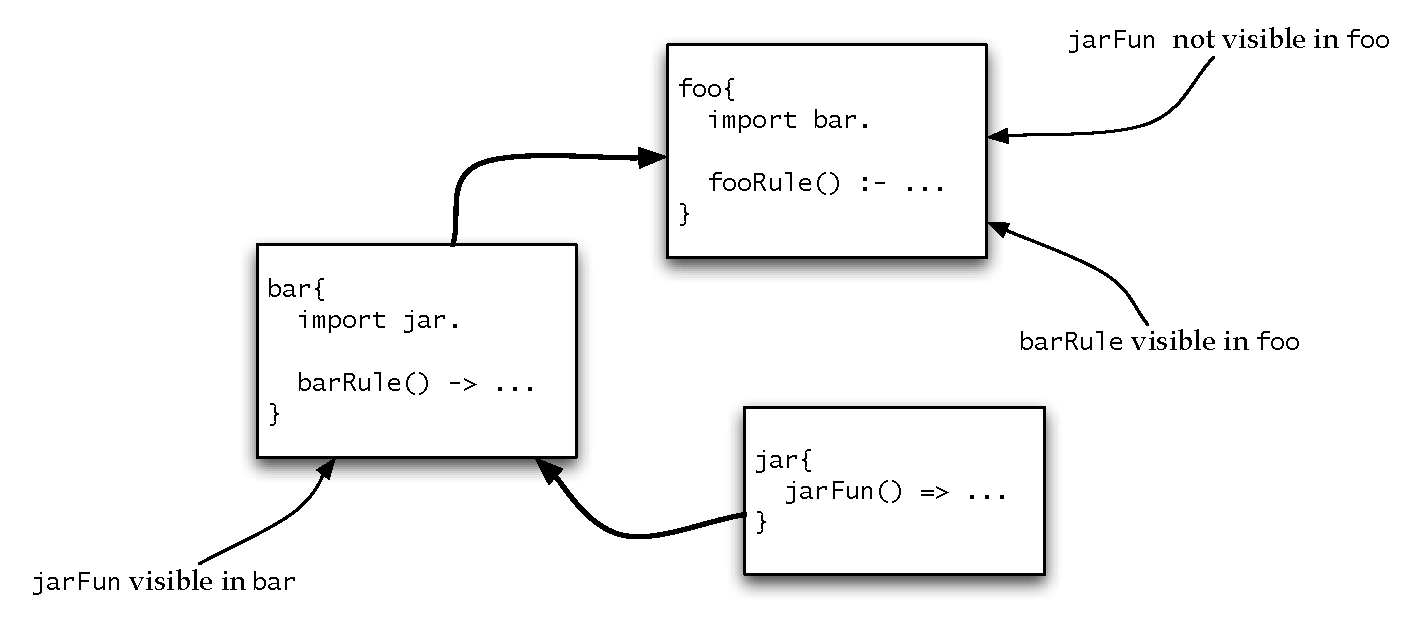
\includegraphics[width=\textwidth]{packages}
\caption{A three-way package \q{import}}
\label{program:packages:imports}
\end{figure}
It is possible for a package to \q{import} a package that, in turn, \q{import}s other packages. These latter packages will be automatically loaded as needed. However, the definitions in these dependent packages are \emph{not} automatically made available to the original \q{import}er. For example, figure~\vref{program:packages:imports} illustrates a case with three packages: \q{foo}, \q{bar} and \q{jar}.
In this scenario \q{jarFun} is available within the \q{bar} package, but not in the \q{foo} package -- even though loading the \q{foo} package will cause \q{jar} to be loaded. If \q{jarFun} is required directly within the \q{foo} then it will have to be explicitly \q{import}ed by the \q{foo} package. Of course, the \q{barRule} action procedure is available within the \q{foo} package.

This can become an issue for type and other definitions that are shared over many packages. In that situation, the shared definitions will need to be \q{import}ed in each context that they are required.

\begin{aside}
One workable technique, as used in our meta interpreter in Chapter~\ref{vmeta}, is to place commonly used types in a package of their own. Then, this type package may be \q{import}ed as needed.
\end{aside}

\index{circular chains of \q{import}s}
\index{package!recursive \q{import} not permitted}
\paragraph{Compiling packages}
The \go compiler requires that a package be compiled (see section~\vref{first:compiling}) before it can be imported; more specifically the compiler searches for the compiled package when compiling a package that \q{import}s a package. Thus, it may be important to ensure that dependent packages are compiled after the packages that they depend on. It is not permitted to have a circular chain of package \q{import}s -- with one package importing another, which in turn causes the original to be imported.

\subsection{Package reference}
\label{package:reference}
\index{operator!\#@\hash}
\index{package!reference}
\index{identifier!package reference}
There are occasions when it is necessary to identify \emph{which} package a particular identifier comes from. The primary purpose here is to resolve the situation where two packages export the \emph{same} identifier; in which case it is not defined which import is respected.

To precisely identify the package for a particular use, we use a \q{\hash} operator:
\begin{alltt}
go.io#stdout
\end{alltt}
The package name on the left is the name of the package -- as it is mentioned in the associated package \q{import} statement. The identifier on the right is one of the identifiers exported by the package.

\section{Top-level main programs}
\label{program:top-level}
Any package can also be treated as the top-level program -- provided that the package has a definition for the single argument action procedure \q{main}. In fact, \q{main} is a reserved keyword in \go: if a \q{main} program is defined in a package then it \emph{must} be consistent with the type assertion:
\begin{alltt}
main:(list[string])*
\end{alltt}
\index{main@\q{main} program}
\index{executing a \go program}

If a package is executed at the top-level, then the \q{main} program in that package is executed and given as its single argument a list of the command-line arguments specified in the execution. For example, if a package \q{foo} were mentioned as the top-level package to execute in:
\begin{alltt}
\% go foo a b c
\end{alltt}
then the package \q{foo} must have an appropriate definition for \q{main} and that action procedure is entered -- with argument the list
\begin{alltt}["a","b","c"]\end{alltt}
\begin{aside}
Since the command line arguments are passed in as \q{string}s it is common for these argument strings to be parsed before they can be used in the application proper.  

\index{operator!\%\%@\q{\%\%}}
The \q{\%\%} parse expression (see page~\pageref{expression:grammarexp}) and the \q{go.stdparse} package become handy in this situation. For example, to pass a numeric value to a \go fragment, where the number comes from the command line itself, then the classic way to do this is:
\begin{alltt}
mainPackage\{
  import go.stdparse.
  
  \ldots
  main([Arg,..More]) ->
    appProg(numeric\%\%Arg);\ldots
\}
\end{alltt}
The \q{numeric} grammar program parses a string into a \q{number} value.
\end{aside}

\section{Standard Packages}
\index{package!standard}
\index{standard packages}
Much of the functionality of the \go system is encapsulated in special packages that are distributed with the \go system. These are generally not automatically included in every program. By convention, all \go system packages have package names of the form: \q{go.\emph{name}}; for example, the system input/output package is called \q{go.io}. To access the standard I/O package, then, it is necessary to load the \q{go.io} package:
\begin{alltt}
\emph{yourpackage}\{
  import go.io.
  
  \ldots
\}
\end{alltt}
\begin{aside}
Input and output are, of course, fairly prevalent in programming. However, the reason that \q{go.io} is not automatically included in every package is that that permits non-standard I/O systems to be used - for example in embedded applications, or in systems which have to interact with file systems in special ways.
\end{aside}
The standard set of packages will vary from time to time, the current set includes the packages
\begin{description}
\item[\q{go.cell}] Implements a re-assignable resource entity.
\item[\q{go.datelib}] Implements a collection of date related functions.
\item[\q{go.dynamic}] Implements dynamic relations; relations that can be updated.
\item[\q{go.hash}] Implements a hash-table package.
\item[\q{go.io}] Implements the standard I/O package
\item[\q{go.mbox}] Implements an internal thread communication package.
\item[\q{go.setlib}] Implements a collection of set-like functions.
\item[\q{go.sort}] Implements a sort function
\item[\q{go.stack}] Implements a shareable updatable stack package.
\item[\q{go.queue}] Implements a shareable updatable queue package.
\item[\q{go.stdlib}] The standard \go language support package. This package is automatically loaded as it is required for successful execution of any \go program.
\item[\q{go.stdparse}] Implements a range of parsing functions, allowing the conversion of strings to numbers, for example.
\item[\q{go.unit}] Implements a unit-testing framework.
\item[\q{go.xml}] Implements an XML parser and displayer package. Also defines the \go version of the DOM (Document Object Model).
\item[\q{go.goweb}] A simple Web server written in \go.
\end{description}






%\chapter{Message communication}
\label{message}

One of \go's standard packages is the message communication package -- \q{go.mbox}.


A client registers a description with the directory with a registration message by sending a \q{register} message to the directory:
\begin{alltt}
register(
   [attr('name',??("sally")),attr('role',??("dancer")),
    attr('gender',??(female))]) >> DS
\end{alltt}
The general form of a message send action is:
\begin{alltt}
\emph{Msg} >> \emph{handle}
\end{alltt}
where \emph{Msg} is any legal \go term, and \emph{handle} is the identity of a \go \emph{mailbox}. 

This is an action, executed in the context of an action rule or other action sequence, and its effect is to send the term:
\begin{alltt}
register(
   [attr('name',??("sally")),attr('role',??("dancer")),
    attr('gender',??(female))])
\end{alltt}
to the mailbox channel held in the variable \q{DS}.

Threads are identified in \go using process \q{handle}s. Thread handles use the \q{hdl} constructor term which has two arguments: the \emph{root} name of the thread and the \emph{thread} identifier -- both are \q{symbol}s. For example, our directory server might have the handle:
\begin{alltt}
hdl('server','directory')
\end{alltt}
where \q{'directory'} is the root name and \q{'server'} is the thread name of the handle. Normally a thread \q{handle} is automatically generated, however it is also possible to manually construct one; in this case that will be useful to permit clients to `know' what process the directory server is.

Program~\vref{dir:publish} shows a simple example of a client program publishing a description with a directory server with a well-known name.
\begin{program}
\begin{alltt}
publish .. \{
  publish() ->
    register(
   [attr('name',??("sally")),attr('role',??("dancer")),
    attr('gender',??(female)),
    attr('name',??(self))]) >> hdl('server','directory').
\}
\end{alltt}
\caption{A client that publishes\label{dir:publish}}
\end{program}
Our directory server is particularly simple-minded: it will accept a publication from anyone, and will not send back any response to the publishing client.








\index{inter-thread communication}
\index{message!based communication}
\index{sending and receiving messages}
Message passing is the main way that \go permits threads, even spawned sub-threads, to communicate with each other.  Note that the reason for this is that debugging and verifying programs with `hidden' side-effects (via the shared data base) is considerably more difficult than when using explicit message passing. In addition, shared values are impractical when the threads are not on the same host; thus direct memory sharing systems are not transparent to the location of the parallel threads.

\subsection{Message send}
\label{action:send}
\index{message!sending}
\index{action!message send}
A message is sent from one thread to another by means of the {\tt >>} built-in action. A message send action takes the form:
\begin{alltt}
\emph{Term} >> \emph{To}
\end{alltt}
where \emph{Term} is the message to be sent to process \emph{To} -- which is a \q{handle}.

\go does \emph{not} require that the message sent be ground; however it \emph{does} require that the type of the message is ground. The reason for this restriction is that the message is implicitly encapsulated as an \q{any} value.

Note, however, that the target of a message send \emph{must} be ground; otherwise the \go system cannot deliver the message to an unknown recipient.

The sending process is given no immediate response to a message send; unless the sender process does not have permission to send messages. If required -- which is often -- the sender should wait for a response using a message receive action. 

\subsection{Message receive}
\label{action:receive}

\index{message!receiving}
\index{action!message receive}
\index{receiving messages}
\index{thread message queue}
A message can be retrieved from a thread's message queue using
a \firstterm{message receive}{A message receive action is one that completes by receiving a message of the correct form; and removing it from the thread's message queue.} action. A message receive action takes the form:
\begin{alltt}
( \emph{P\sub1} << \emph{F\sub1} -> \emph{A\sub1}
| 
| \emph{P\subn} << \emph{F\subn} -> \emph{A\subn}
)
\end{alltt}
where each \emph{P\subi} indicates a message pattern to receive and the corresponding \emph{A\sub{i}} the action to take on receiving such a message. Note that the parentheses around the message rules are necessary in a message receive action.

The \q{P\subi} are the \emph{guards} of the receive clauses. The entire message receive completes if there is a message in the message buffer that matches one of the \q{P\subi} patterns. The message queue of the process will be scanned from the beginning looking for such a message, and the patterns will be tested against each message in the buffer in the order in which they are given.

As soon as a message is found that satisfies one of the guards, the message is removed from the message buffer and the corresponding \q{A$_i$} of the message receive clause is executed. There is no backtracking on the selection of the receive clause or the removal of the message.

A message receive choice never fails. If it does not succeed with the current contents of the message queue it suspends until a  message arrives that satisfies one of the message rule guards.  Suspension waiting for an acceptable message is the primary form of thread control in \go.

The degenerate form of message receive, where there is only one message rule, and its body is empty, corresponds to the simple message receive:
\begin{alltt}
( \emph{Msg} << \emph{sender} -> \{\} )
\end{alltt}
can be replaced by:
\begin{alltt}
\emph{Msg} << \emph{sender}
\end{alltt}
in the body of an action rule.

\index{message!guards in message receive}
Guarded terms are often useful in the context of a message receive: they can be used to extend the pattern with semantic as opposed to purely syntactic conditions. For example, the message receive action:
\begin{alltt}
\ldots;(N::N<Q) << S;\ldots
\end{alltt}
looks for a \q{number} from sub-thread \q{S} whose value is less than the value of the variable \q{Q}. Numeric messages that are greater than \q{Q}, or messages from sub-threads whose \q{handle}s do not unify with \q{S}, will \emph{not} be picked up by this message receive.

\subsubsection{Timeouts in message receive}
\index{message!timeout}
\index{Timing out a message receive}

It is possible to `time out' a message receive -- by using a special form of message receive rule: the \q{timeout} clause. The form of a message receive with a timeout is:
\begin{alltt}
(\emph{MsgRule\sub1} | \ldots{} ) timeout (\emph{TimeExp} -> \emph{TimeOutAction})
\end{alltt}
If there is no message that matches any of the guarded patterns in \emph{MsgRule\subi} by the time that \emph{TimeExp} seconds has expired, then the message receive `times out' and the \emph{TimeOutAction} is executed. The \q{timeout} expression refers to a number of seconds (it may be fractional) of real elapsed time; it does not refer to processor time.

The start time of time-out is calculated from just before there is any attempt to read any messages; and the timeout is invoked only if there are no messages in the message queue -- at the time that the message receive is entered -- that match any of the patterns. I.e., if there is a message in the message that matches one of the patterns, then the timeout clause is effectively ignored. Setting the \q{timeout} to 0 seconds is effectively `peeking' at the message queue to see if there is currently a matching message.

\emph{Warning:}
\begin{quote}
\index{Why \q{timeout}s are bad for your program's health}
Using \q{timeout} clauses without care in the choice of timeout values is likely to result in programs that have bugs that are hard to detect -- since there is always some non-determinism in the order of execution in multi-threaded applications. Furthermore, especially for networked applications, computing the appropriate values to assign for timeouts is likely to be problematic given the enormous variation in network latency delays.
\end{quote}

\paragraph{Semantics of message receive}
Message receives involve a search of the message buffer -- it is not required that the first message in the queue matches. If a later message matches then the intervening messages are retained in the message queue for subsequent retrieval. This allows a process to receive messages from any process while continuing to focus on only those messages of immediate interest.\note{This is a similar message handling model to that of {\tt April} and {\tt Erlang}.}

One might ask if there is a relationship between message receive and \q{sync}hronized action. After all, the message queue associated with a thread does represent a shared resource: other threads write messages to the end of the queue and the message queue's owner thread reads from the front of the queue. Even the message receive choice action is reminiscent of the choice \q{sync} action.

While it \emph{is possible} to construct a mapping of \go's message receive choice in terms of \q{sync} actions, it is complex. The reason is that the various choices in a message choice are considered in parallel: for each message in the queue, each of the alternatives is considered. Only if none of the message choices patterns fires do we move on to consider the next message in the queue. On the other hand, \q{sync} actions would naturally considers the various choices \emph{sequentially}: the first rule that fires for \emph{any} message in the queue will fire. However, that form of message receive semantics leads to a kind of unfair search in the message queue that can lead to hard to find bugs.



  


%\part{Programming in \go}
%\label{agentProgramming}
%\chapter{Planning with STRIPS}
\label{strips}

A key element of many agent applications is the planning of a sequence of actions. This is often broken down into two phases: constructing a plan and executing it. These are related in that often well intentioned plans do not work as advertised; and therefore when executing a plan the preconditions for some or all of the actions may need to be verified, and re-planning may be required. 

In this chapter we look at implementing one of the classic approaches to planning -- namely a STRIPS planner. The STRIPS style of planner assumes a world of discrete actions, discrete goals and observable properties of the world. Each action is characterized by the set of facts that it `adds' to the world -- i.e., makes true if the action is successful -- and the set of facts that it deletes -- i.e., makes false if the action is unsuccessful. Each action is also associated with a set of pre-conditions -- observed properties of the world that must be true for the action to have meaning.

For example, in the blocks world, picking up a block requires that the block is clear -- no block is stacked on top of it -- and that its on the table. If the pickup is successful, then it will no longer be on the table, and will no longer be clear -- in the sense that its not possible to stack blocks `in the hand'; and so \q{clear} really means that it is permitted to stack a block on top of it.
\begin{aside}
Another key assumption in the STRIPS model is that there are no other active agents in the world that can also act. This assumption is clearly invalidated in any multi-agent scenario; however, for an agent planning its internal activities the single-actor assumption is often reasonable.
\end{aside}

\section{Robbie's world of blocks}
\label{strips:blocks}
Our demonstration of our planner is the classic one of a robot -- called Robbie -- being able to manipulate blocks: by picking them, stacking and unstacking and so on.
\begin{aside}
This world should not be confused with anything realistic. However, it's primary purpose here is show how knowledge about a specific domain is integrated with a generic planning engine.

For example, we do not attempt to address how Robbie might be able to perceive that a given block is stacked on another. This is a non-trivial problem, requiring typically the ablity to interpret a scene via a video camera.
\end{aside}
For the simple blocks world the \q{blockActs} type captures the range of available actions:
\begin{alltt}
blockActs ::= stack(symbol,symbol)
    | unstack(symbol,symbol)
    | pickup(symbol)
    | putdown(symbol).
\end{alltt}
we use symbols to identify the various blocks we may encounter.

The \q{blockPred} type names the possible predicates in the blocks world:
\begin{alltt}
blockPred ::= clear(symbol)
    | holding(symbol)
    | ontable(symbol)
    | on(symbol,symbol)
    | handempty.
\end{alltt}
In effect, we are limited to sensing whether a block is \q{clear}, whether it is on the table and so on. Other potentially important properties of blocks, such as their shape, size, weight, color and so on, are not modeled here. Although it would be a relatively simple extension to do so, the art of designing and effective system lies as much in what we \emph{do not} design as in what we do construct.

Just as we simplify the potential properties of blocks, the possible actions that the execution engine (a.k.a. blocks world robot) can take is also simplified: it is possible to stack blocks on top of each other, to unstack a block from a stack, to pick up a block, and to put it on the table. These actions are quite high-level from the perspective of a physical device manipulating real blocks; these actions would have to be broken down into simpler activations of the robot's mechanical muscles.

\subsection{The \q{stripsWorld} interface}
\label{strips:world}
The \q{stripsWorld} type definition:
\begin{alltt}
stripsWorld[A,G] \impl \{
  strips_rule:[A,list[G],list[G],list[G]]\{\}.
\}.
\end{alltt}
expresses the contract that the domain-specific part of the system must fulfill. In order for the generic planner to be able to know what the legal operations are in a given domain, it is given a class that implements this type. The \q{strips\_rule} predicate defines the planning operators themselves.

Note that \q{strips\_rule} is a predicate and not a function because a given set of goals may have more than one action associated with it. It is not permissible for the same action to be mentioned in more than one \q{strips\_rule} clause: that would imply that the action had more than one set of preconditions and consequences.

\subsection{The blocks planning domain}
Our \q{robbie} class, in Program~\vref{strips:robbie}, captures Robbie's possible actions in the world as rules in the \q{strips\_rule} relation.
\begin{program}
\vspace{0.5ex}
\begin{alltt}
robbie\{
  import go.setlib.
  import strips.

  robbie:[]\conarrow{}stripsWorld.
  robbie..\{
    strips\_rule(stack(X,Y),
              [clear(Y),holding(X)],
              [on(X,Y),clear(X),handempty],
              [clear(Y),holding(X)]).
    strips\_rule(unstack(X,Y),
              [on(X,Y),clear(X),handempty],
              [clear(Y),holding(X)],
              [on(X,Y),clear(X),handempty]).
    strips\_rule(pickup(X),
              [ontable(X),clear(X),handempty],
              [holding(X)],
              [ontable(X),clear(X),handempty]).
    strips\_rule(putdown(X),
              [holding(X)],
              [ontable(X),clear(X),handempty],
              [holding(X)]).
  \}.
\}
\end{alltt}
\vspace{-2ex}
\caption{Operators in Robbie's world}
\label{strips:robbie}
\end{program}
Each \q{strips\_rule} in the \q{robbie} class defines the preconditions of the action, the positive effects on the world and the negative effects. For example, the \q{stack} action requires that the block is in the hand of the robot and that the target is \q{clear}. The positive effects are that the newly stacked block is \q{clear} and that the robot's hand is empty. The negative effects are that the target block is no longer \q{clear} and that the robot is no longer \q{holding} the stacked block.\note{For the sake of clarity and simplicity we have assumed that the planner will only plan using primitive actions.}

Although the modeled world of blocks is not permitted to contain predicates with variables, there is no such restriction on the description of the action rules; nor on possible descriptions of the modeled world. This permits \go's descriptions of the possible actions to be very compact; while at the same time simplifying the logic of the modeled world.

Other domains would have different actions, with a different language of conditions. For example, an application in terms of eCommerce might have actions around searching for suitable vendors and purchasing goods.

Note that Program~\vref{strips:robbie} defines the range of actions as a `fixed' relation; but there is nothing intrinsic in this. One might wish to extend this to include a more dynamic, learnable, range of actions.

\section{A simple STRIPS planner}
\label{strips:strips}

Program~\vref{strips:planner} shows a simple planning program that uses a \q{strips\_rule} database as its source of actions. This program should not be considered to be a sophisticated planner: it is more of a specification than an effective algorithm.
\begin{program}
\vspace{0.5ex}
\begin{alltt}
strips\{
  planner[A,G] \impl \{
    plan:[list[G],list[G]]=>list[A]
  \}.

  stripsWorld[A,G] \impl \{
    strips_rule:[A,list[G],list[G],list[G]]\{\}.
    holds:[G]\{\}.
    do:[A]*.
  \}.

  stripsPlanner:[stripsWorld[A,G]]\conarrow{}planner[A,G].
  stripsPlanner(W:stripsWorld[A,G])..\{
    plan(Init,Goal)::strips(Init,Goal,[],Plan) => Plan.

    -- This is a progressive planner,
    -- planning forwards from the state to the goal
    strips:[list[G],list[G],list[A],list[A]]\{\}.
    strips(State,Goal,_,[]):-
      subset(Goal,State).
    strips(State,Goal,Forbidden,[Ac,..Plan]) :-
      W.strips_rule(Ac,Prec,Adds,Dels),
      subset(Prec,State),
      \nasf{} Ac in Forbidden,
      strips((State\union{}Adds)\difference{}Dels,Goal,[Ac,..Forbidden],Plan).
   \}.
  \}
\}
\end{alltt}
\vspace{-2ex}
\caption{A simple STRIPS planner}
\label{strips:planner}
\end{program}
The main part of this program is the \q{strips} relation defined within the \q{stripsPlanner} class. The first \q{strips} rule says that we have finished the plan if the set of out-standing goals is already satisfied in the modeled state of the world. A goal is satisfied  by being in the state.

The second \q{strips} clause picks an action operator whose pre-conditions have been met, and whose action has not yet been tried, and plans forward from there.

Note that the state is represented as a pair: a set of facts that is true in the state and a current list of \q{Forbidden} actions. This latter list is there to avoid loops of actions being repeated forever.

The somewhat complex expression:
\begin{alltt}
(State\union{}Adds)\difference{}Dels)
\end{alltt}
computes a new state in terms of the intermediate state arrived at by performing the action, and a list of new facts -- the \q{Adds} -- that are now true and the list of removed facts -- \q{Dels} -- that are no longer true in the new state.

An expression of the form \q{\emph{A} \union{} \emph{B}} represents the set (represented as a list) of the elements of \q{\emph{A}} unioned with the elements of \q{\emph{B}}. Similarly, an expression of the form: \q{\emph{A} \difference{} \emph{B}} denotes the difference of the two sets. Both the \union{} and the \q{difference} operators are part of the \q{setlib} library that is part of the standard distribution of \go.

This planner directly constructs plans that are valid instances of the \q{actType} type, as defined in Program~\vref{strips:prog-type}. This facilitates the integration of the planner with a possible action executor, a topic we look at in Section~\vref{strips:exec}.

Note that if the planner fails to solve a sub-goal, then a different sub-goal is picked. This has the effect of potentially producing an ordering of actions that is quite different to the original list of goals. It is also one of the greatest sources of inefficiency in the planner -- blindly searching through the space of goals until a particular combination works. More sophisticated planner algorithms, such as goal regression based planners, would attempt to preserve partially successful plans in order to reduce the total cost of planning.

If no plan can be constructed then the \q{plan} function will raisew an \q{"unexpected failure"} error exception; which should be caught by the invoking program.

The algorithm in Program~\vref{strips:planner} has the merit of being short, and easy to explain; it is, however, not really a good example of an efficient planner. However, with the program structure that we have established, it should be relatively straightforward to replace the \q{planner} module with a more sophisticated planner -- a regression planner for example -- without compromising the rest of an application that uses planners.

% \section{Executing plans}
% \label{strips:exec}

% Planning a sequence of action steps is not sufficient to achieve a goal -- the actions must also be performed! Of course, for real-world interactions, it is not guaranteed that an action produces the expected results; furthermore, in the presence of other agents, the world may evolve during the execution of a plan -- with the potential for invalidating some or all of the assumptions made during planning.

% Our task in this section is to develop an \emph{action} interpreter that can execute plans; with possible re-planning when the world no longer matches the expectations of the agent. In Program~\vref{prog-script} we build on the ideas in the meta-interpreter in Chapter~\vref{meta} to construct an execution interpreter.

% \begin{program}
% \vspace{0.5ex}
% \begin{alltt}
% execPlan\{
%   import go.io.
%   import planAct.
%   import strips.

%   runPlan[A,G]\impl\{
%     exec:[planAct[A,G]]*.
%   \}.

%   planRun:[world[A,G]]\conarrow{}runPlan[A,G].
%   planRun(W)\{
%     exec(prim(Prec,Act)::W.holds(Prec)) -> W.do(Act).
%     exec(single(G,_)) -> exec(W.plan(G)). -- replan
%     exec(seq(L)) -> E in L *> exec(E).
%     exec(choice(Tst,A1,_)::W.holds(Tst)) -> exec(A1).
%     exec(choice(_,_,A2)) -> exec(A2).
%     exec(subplan(Name)) -> exec(W.which(Name)).
%   \}
% \}
% \end{alltt}
% \vspace{-2ex}
% \caption{A simple script executor}
% \label{prog-script}
% \end{program}

% The first action rule for \q{exec} executes a \q{prim}itive action by requesting that the `world' object -- represented by the \q{W} argument of \q{run} -- execute the action. However, it only does so if the required precondition still holds: in the real world not all actions are successful, and, furthermore, other agents may have caused interference with the world view.

% In the event that the required precondition does not hold anymore, the planner is invoked on the original precondition to see if an alternate plan can be constructed. This is a very simplistic approach to recovery; as it may be that a higher-level goal needs to be reconsidered. A better approach may be to set specific recovery points that the executor would re-plan from.

% The other rules for \q{exec} are straightforward: we execute a sequence by iterating over the elements of the sequence, we execute a \q{choice} by considering the test, and we execute a \q{subplan} by retrieving the plan and executing it.

%\chapter{Fun with mobile agents}
\label{mobile}
\index{Mobile agent}
\index{Agent!mobile}

\go is not intentionally designed to make programming \firstterm{mobile agents}{A \emph{mobile agent} is a program that can propagate itself to execute on different hosts. The difference between a mobile agent and a virus is that normally mobile agents require special host support -- and a difference in intent.}  easy; however, as we shall see, it is not difficult to do. The reason is that a combination of message passing and programs being first class entities naturally leads to a straightforward technique for implementing mobile agents.

\paragraph{Don't do this at home}
First of all a warning: the difference between a mobile agent and a virus is often very slight: it is a matter of intention. The mobile agents that we will write here though are different to viruses in the sense that they require active support of the host: without a \emph{very} cooperative host, our mobile agents will be dead on arrival.

\section{The elements of a mobile agent}
The core features of \go that make programming mobile agents easy are the fact that programs are first class entities and message passing. The combination of these means that we can pass programs in messages. It is a short step from passing a program in a message to a mobile agent: all that is required is the ability and willingness of the recipient of the message to execute the received program.

\index{mobile agent!recursive form}
Program~\vref{mobile:p1} is a simple agent program that will attempt to propagate itself.
\begin{program}
\begin{alltt}
mobile .. \{
  include "sys:go/stdlib.gof".
  include "sys:include/io.gh".

  mbProto ::= exec((outFile[])*).

  mobile([]) -> \{\}.
  mobile([P,..laces]) ->
    exec(((Oc)->Oc.outLine("I am "{}<>self^0);
                mobile(laces)))>>P.
\}
\end{alltt}
\caption{A simple mobile agent\label{mobile:p1}}
\end{program}
The \q{mobile} action procedure has a single argument -- a list of `places' to visit. In the case that the list is empty then the \q{mobile} action will simply terminate.\sidenote{Again, a notable distinction between our mobile programs and viruses.} In the case that the list is non-empty, then the action body of the second rule is to send the message:
\begin{alltt}
exec(((Oc)->Oc.outLine("I am "{}<>self^0);mobile(laces)))
\end{alltt}
to the process identified by the first element of the list. The \q{exec} constructor is defined in the type definition:
\begin{alltt}
mbProto ::= exec((outFile[])*).
\end{alltt}
\q{exec} has a single argument -- which is a single argument action procedure. The argument of this single argument procedure is \q{outFile[]}, which is the standard type denoting an output file channel. When it is executed, this procedure will be given an object which the mobile agent can use to write messages.

In our case, the argument to the \q{exec} message we send is a single-argument procedure:
\begin{alltt}
(Oc)->Oc.outLine("I am "{}<>self^0);mobile(laces)
\end{alltt}
This procedure, when executed, displays a message on the output channel given in the argument \q{Oc}, and then proceeds to invoke the \q{mobile} action procedure with the remaining elements of the list of places to visit.

Notice that without being passed the output channel there is no possible way for the mobile agent to display any messages. Although \go supports mobile agents, it also makes it very easy to control them: any resources that a mobile agent uses must be passed explicitly into the program when it is executed.

The stages that our mobile agent will go through are:
\begin{enumerate}
\item It will be executed by some host. When it is executed, the object that denotes the resources it may use are passed in to it; in our case, the only resource permitted is an output channel for writing text.

\item Once initiated, the mobile agent uses the resource given to it to display a message: ``I am here''.

\item After displaying the message, the agent calls the \q{mobile} program; with a list of places to go to.

\item The \q{mobile} action procedure picks the first of those places and sends it a message. The message contains the mobile agent itself; and therefore the cycle continues.
\end{enumerate}
This two-phase structure is quite typical for mobile agents: it is as though the mobile agent has two phases in its life-cycle: an active phase when the agent code can more-or-less do what it wants and a `spore' phase when the agent is packaged as a standard message that can be accepted by suitable hosts.

Note that although \go can send programs in messages, it is \emph{not} the case that all values are first class. In particular, it is not permitted to send objects that reference other system resources -- such as file channels. Any attempt to do so will result in an \q{error} exception when the message send is attempted.


\subsection{An Object oriented mobile agent}
\label{mobile:object}
\index{mobile agent!object oriented}
One of the obvious limitations of the mobile agent in Program~\vref{mobile:p1} is that it cannot easily carry any reasonable form of \emph{state}. This is because the agent is couched in hte terms of a simple two-phase recursion, with the only state being represented in the arguments to the \q{mobile} call. In Program~\vref{mobile:o1} we show a slightly different form of mobile agent that is encapuslated as a class; which \emph{does} permit state.
\begin{program}
\begin{alltt}
mobile..\{
  include "sys:go/stdlib.gof".
  include "sys:go/io.gof".
  include "sys:go/stack.gof".
  include "sys:go/cell.gof".
  include "mobile.gh".

  mobile[]\impl{}mbAgent[].        -- We are a mobile agent 
  mobile(l,home)\{
    Places = \$stack[handle](l).   -- List of places to go
    Counter = \$cell[number](0).   -- Count visited places

    visit(P) ->         -- We might get a request to visit
        Places.push(P).

    exec(\_)::Places.depth()==0 -> this>>home.
    exec(O:outFile) ->
        O.outLine("I am "{}<>this^0<>" at my "{}<>
                  Counter.get()^0<>"th place");
        Places.pop(Nx); O.outLine("Going to "{}<>Nx^0);
        Counter.set(Counter.get()+1);
        this >> Nx.
  \}
\}
\end{alltt}
\caption{A \q{mobile} class}
\label{mobile:o1}
\end{program}
This program has a number of features that distinguish it from \q{mobile} in Program~\vref{mobile:p1}:
\begin{itemize}
\item
The class exposes an \q{exec} element; this acts as the \q{mobile} executor: when the object is woken up at a station, then the \q{exec} element will be executed.
\item
\q{exec}uting the object is not the only operation that can be performed on the agent: it can also be asked the object to \q{visit} another station. Although, any such action should be performed \emph{before} the \q{exec} action.
\item
Instead of holding the list of places to visit in an argument of the \q{mobile} action procedure, this list is held in a \q{stack} variable.\footnote{The \q{stack} class is a standard library that implements a simple stack object -- allowing \q{push}es and \q{pop}s.}
\item
The execution of the mobile object is significantly simpler: instead of an iterative recursion where a closure is used to represent the continuation of the mobile agent at the next station, it simply sends the object itself to the next station.
\item
The \q{mobile} class declares that it implements the \q{mbAgent} interface. It is this interface that the support station for the mobile agent will be expecting. The \q{mbAgent} interface is defined to be:
\begin{alltt}
mbAgent[] \cast \{
  exec:(outFile[])*.
  visit:(handle)*.
\}.
\end{alltt}
We have assumed that this interface is defined in the file \q{mobile.gh}.
\item
It is very natural to incorporate additional state elements in the object -- as simple \q{cell} objects or even more complex \q{dynamic} relations.
\end{itemize}

\section{A mobile agent support system}
\label{mobile:base}
\index{Mobile agent!base station}
\index{Base station for mobile agent}
\index{Agent!base station for mobile}

In order for our mobile agent to execute it must go through the critical step of being executed. This is not something that the mobile agent can do by itself -- sending a message with a program in it is not the same as actually executing the program.

In order to complete its life-cycle, the mobile agent needs a host that is willing and able to execute it. In particular, when it receives a message with the mobile agent code in it, the host must call it; perhaps by \q{spawn}ing a new sub-thread.
\index{|q{spawn} sub-thread}

In addition to executing the mobile agent, our host must also pass in to the code an output file channel object. In our case, we will simply pass in to the agent the local \q{stdout} file channel. Program~\vref{mobile:base1} is a simple base station that \q{spawn}s a new thread whenever it receives an \q{exec} message.

\begin{program}
\begin{alltt}
base .. \{
  include "sys:go/io.gof".
  include "sys:go/stdlib.gof".

  include "mobile.gh".

  base() ->
      ( A\impl{}mbAgent[] << \_ -> spawn \{ A.exec(stdout)\});
      base().
\}.
\end{alltt}
\caption{A base station for \q{spawn}ing mobile agents\label{mobile:base1}}
\end{program}
The \q{base} program is very trusting: it waits for a message consisting of any object that implements the \q{mbAgent[]} interface, and simply \q{spawn}s a new thread whose sole task is to execute the \q{exec} method in that object -- passing into it the local \q{stdout} file channel object -- and then goes on to wait for the next \q{exec} message.

Of course, in general, we should augment the \q{base} program to perform validation checks on the incoming message; such as verifying the sender, perhaps even entering into a conversation with the sender -- looking for a security certificate for example. One way of doing this might be to extend the \q{mbAgent} interface, and to challenge the object with some query.

Notice that the base station does not know what the mobile agent is going to do. However, it does limit the mobile agent by only passing to it the resource that the host is willing for the guest program to use.

\section{Mobile agents in a teacup}
We can test our mobile agents and base station by arranging for the agents to move around a set of base stations located entirely within a single invocation of \go. Program~\vref{mobile:teacup} is a harness program that \q{spawn}s four base stations -- \q{B1} \ldots \q{B4} -- and two unnamed mobile agents. The two mobile agents traverse our network of base stations -- in a different order -- and `return' back to the main thread.

\begin{program}
\begin{alltt}
main .. \{
  include "sys:go/io.gof".
  include "sys:go/stdlib.gof".
  include "mobile.gh".
  include "mobile.gof".
  include "mbase.gof".

  main() ->
      B1 = spawn \{ base() \};
      B2 = spawn \{ base() \};
      B3 = spawn \{ base() \};
      B4 = spawn \{ base() \};
      A1 = \new{}mobile[]([B1,B2,B3,B4,B1,B2,B3,B4],self);
      A2 = \new{}mobile[]([B1,B2,B3,B4,B1,B2,B3,B4],self);
      spawn \{ A1.exec(stdout) \};
      spawn \{ A2.exec(stdout) \};
      ( AA\impl{}mbAgent[] << \_ ->
            stdout.outLine(AA^0<>" has come home")
      );
      ( BB\impl{}mbAgent[] << _ ->
            stdout.outLine(BB^0<>" has come home")
      );
\}
\end{alltt}
\caption{A teacup full of mobile agents\label{mobile:teacup}}
\end{program}

We arrange the mobile agent's route by seeding the agent with a list of stations to visit, ending with ourselves.

If we run our program, we get an output similar to:
\begin{alltt}
go teacup.goc
I am \$mobile7177431163697380936 at my 0th place
Going to hdl('computer#764608905.1','computer#764608905')
I am \$mobile7177431163697380936 at my 1th place
Going to hdl('computer#764608905.2','computer#764608905')
I am \$mobile7177431163697380936 at my 2th place
Going to hdl('computer#764608905.3','computer#764608905')
I am \$mobile7177431163697380936 at my 3th place
Going to hdl('computer#764608905.4','computer#764608905')
\ldots
\$mobile7177431163697380936 has come home
I am \$mobile7061765529752583752 at my 5th place
Going to hdl('computer#764608905.2','computer#764608905')
I am \$mobile7061765529752583752 at my 6th place
Going to hdl('computer#764608905.3','computer#764608905')
I am \$mobile7061765529752583752 at my 7th place
Going to hdl('computer#764608905.4','computer#764608905')
\$mobile7061765529752583752 has come home
\end{alltt}


\section{Mobile agents in a larger world}
\index{mobile agent!distributed}
Shuttling programs between threads in a single invocation can hardly be called genuine mobile agents. However, with a little extra effort, we can transform Program~\vref{mobile:teacup} into a genuine mobile agent scenario.

To complete the picture we need to have a way for base stations to be executing in different invocations of \go -- potentially on different machines -- and for these base stations to communicate. To facilitate this we can use the SCS -- the Simple Communications System (see Section~\vref{scs:setup}).

Program~\vref{mobile:station} shows how we can use the \q{base} code from Program~\vref{mobile:base1} as the basis of a mobile agent \emph{station} -- in the context of the SCS.
\begin{program}
\begin{alltt}
main..\{
  include "sys:go/scomms.gof".
  include "base.gof".

  main(Host) -> scsConnect(base,Host,5050).
\}
\end{alltt}
\caption{Creating a base station that is connected to the SCS\label{mobile:station}}
\end{program}
When \emph{this} program is run, it will connect to the \q{scs} server executing on the host identified in the \q{host} argument and register itself with it. This will allow other programs (i.e., the mobile agents) to send the base station messages.

This program is designed to be executed with explicit command line options that tell the \go engine what the top-level \q{handle} of the base station should be. We will need this when we initiate the mobile agents themselves. For now, let us assume that there will be four base stations set up: \q{A}, \q{B} and \q{C}:
\begin{alltt}
\% go -N A -n base station.goc Ariel.local&
\% go -N B -n base station.goc Ariel.local&
\% go -N C -n base station.goc Ariel.local&
\end{alltt}
All of this assumes, of course, that the \q{scs} is executing on port 5050 on the machine \q{Ariel.local} -- the individual base stations themselves do not need to execute on the same computer.

To start a mobile agent off, we also need to execute it in the context of a program that has been connected to the \q{scs}. Program~\vref{mobile:start} is a simple example of how to do this.

\begin{program}
\begin{alltt}
main..\{
  include "sys:go/scomms.gof".
  include "sys:go/io.gof".
  include "sys:go/stdlib.gof".
  include "mobile.gh".
  include "mobile.gof".

  start() ->
      A = \$mobile([hdl('base','A'),hdl('base','B'),
                    hdl('base','C')],self);
      A.exec(stdout);
      loop() .. \{
        loop() -> (
             XX\impl{}mbAgent[] << From ->
                 stdout.outLine(XX^0<>" has come home");
                 XX.visit(hdl('base','A'));
                 XX.visit(hdl('base','B'));
                 XX.visit(hdl('base','C'));
                 XX.exec(stdout)  -- start agent on new journey
            ); loop()
      \}.
  main() -> scsConnect(start,"localhost",5050).
\}
\end{alltt}
\caption{A mobile agent home\label{mobile:start}}
\end{program}
As with the \q{station} program in Program~\vref{mobile:station}, we start the agents by executing the command:
\begin{alltt}
\% go home.goc Ariel.local
\end{alltt}

Program~\vref{mobile:start} is similar in spirit to Program~\vref{mobile:teacup}; with a couple of differences: instead of directly \q{spawn}ing the base stations and the mobile agents, we only execute the mobile agent code itself, and we do so in the context of a connection to the \q{scs}. The second difference is that \emph{this} version will send the agent off again when it comes `home', creating an endless loop that is highly reminiscent of computer viruses.

With Program~\vref{mobile:station} we have put into place the final piece necessary for our simple demonstration of mobile agents. The total number of lines of \go code here is a little over 50 lines! It has taken five times that number to explain it. Of course, our mobile agents don't \emph{do} very much when they `get' somewhere; but that is not the point of this exercise.









%\chapter{XML, SOAP and all that}
\label{soap}

Any significant application that interacts over the Internet will be required, at some point, to be able to process XML data. In addition, Web services represent an increasingly important technique for exposing functionality in standardized ways -- i.e., if you want to let other people use your application then offering a Web services-based interface is an important tool for doing so.

\section{\go and XML}
\label{xml:xml}
\index{XML}
\go has a standard library that enables processing in XML, called \q{xml.gof}. This module offers several programs, the most important of which are a grammar to parse a \q{string} as an XML document and a function to display a \q{xmlDOM} tree in XML. The parser is not `full' XML: it does not permit or recognize DTD declarations for example, but it does has support for name spaces. The \q{xmlParse} parser is oriented at processing XML messages and machine-readable documents rather than XML-as-cut-down-SGML documents. 

\part[Appendices]{Appendices}

\appendix
%\chapter{Installing \go}
\label{install}

\lettrine[nindent=0.1em]{T}{his} appendix gives instructions on installing \go and \april on a Unix-based system. It is possible to install and use both on a Windows system, under Cygwin; however this is beyond the scope of this chapter to explain how.

\emph{Warning:}
\begin{quote}
The information in this appendix is subject to change and may be different in your situation.
\end{quote}

\section{Getting \go}
The installation of \go requires the installation of three packages: \q{ooio}, \april and \go proper. For a number of reasons, \go is currently only distributed as source.

The \q{ooio} library is a basic library that supports many functions of the other two packages.

The \april language system is a full programming language. It is used only to compile \go programs, however.

The \go language system is the complete engine, compiler and documentation.

A good place to get the source tarballs for these packages is
\begin{alltt}
http://homepage.mac.com/frankmccabe
\end{alltt}

Assuming that you have the files \q{ooio-\em{date}.tgz}, \q{april-\em{date}.tgz} and \q{go-\em{date}.tgz} then the process involves first of all compiling and installing \q{ooio}, then \april, and then doing a similar job for \go.

\section{Installation directory}
The systems \q{ooio}, \april and \go are designed to be installed by default in the directories \q{/opt/ooio}, \q{/opt/april} and \q{/opt/go} respectively. It is possible to set up both to install in different locations; for example in your home directory. However, we \emph{do not} recommend installing either in the `standard' installation directories \q{/usr/bin} and/or \q{/usr/local/bin}. However, it is certainly possible to install \emph{links} to the \april/\go compilers and run-time systems in those locations.

The installation directory is important as it includes a number of files that are important for the smooth running of both \april and \go.

You can make the appropriate directories in the default locations using:
\begin{alltt}
\% mkdir /opt/nar /opt/april /opt/go
\% chown <yourUserName> /opt/nar /opt/april /opt/go
\end{alltt}

\section{Building the \q{ooio} library}
Unpack the \q{ooio-\em{date}.tgz} file and enter the \q{ooio} top-level directory. The \q{ooio} library is set up to use the \q{configure} script -- which was automatically generated using a combination of \q{automake} and \q{autoconf}. 

To configure \q{ooio} run the \q{autogen.sh} script:
\begin{alltt}
ooio \% ./configure [--prefix=\emph{dir}]
\ldots
\end{alltt}
It is only necessary to supply the \q{--prefix} argument if \q{/opt/ooio} is not the preferred installation directory.

Once configured, compile the library using the \q{make} command:
\begin{alltt}
ooio \% make all
\end{alltt}

If you own the target directory, then you can simply:
\begin{alltt}
ooio \% make install
\end{alltt}
to install it; otherwise, try:
\begin{alltt}
ooio \% sudo make install
\end{alltt}
remembering, of course, that the password the system will ask for is your's, not that of root.

\section{Building \april}
The process to build and install \april is similar to that for the \q{ooio} library; with the additional wrinkle of dealing with a non-standard location for the \q{ooio} library.

Unpack the \q{april.tgz} tarball and enter the \q{april5} directory. 

To configure \april run the \q{configure} script:
\begin{alltt}
april5 \% ./configure [--prefix=\emph{dir}] [--with-ooio=\emph{ooioDir}]
\ldots
\end{alltt}
It is only necessary to supply the \q{--prefix} argument if \q{/opt/april} is not the preferred installation directory, and the \q{--with-ooio} argument is only needed if you installed \q{ooio} in a non-standard place.

Once configured, compile \april and install it using the \q{make} command:
\begin{alltt}
april5 \% make all install
\end{alltt}

\subsection{Paths}
Since \april (and \go) are designed to install in their own directories, it is useful to extend the \q{path} environment to include them. You can do this in your \q{.bash\_login} file in your home directory\note{The process for doing this if you use a different shell will be similar.}:
\begin{alltt}
export PATH=\$PATH:/opt/april/bin:/opt/go/bin
\end{alltt}

\section{Building \go}
The process for setting up \go is exactly analogous to that for \april; excepting that if you have installed \april in a non-standard directory, you need to inform \go's configuration script:
\begin{alltt}
go \% ./configure[--with-april=\emph{dir}] [--with-ooio=\emph{ooioDir}]
\end{alltt}

Making \go is also similar:
\begin{alltt}
go \% make
\end{alltt}
There is one additional step in building \go: checking that everything is running Ok. The command:
\begin{alltt}
go \% make check
\end{alltt}
will check out quite a few of the features of \go. If this test does not terminate normally then is there is likely a problem that needs to be sorted out.

Assuming that the test works out, install \go:
\begin{alltt}
go \% make install
\end{alltt}

\section{Setting up EMACS}
The \go system comes with special modes for the GNU EMACS editor.\note{Editor does not do justice to EMACS, it is more like a language/editor/operating system; if a little old-fashioned.}

To access the EMACS mode for \go, you will need to modify your \q{.emacs} file. Just edit that file (in EMACS of course), and make sure that the following lines:
\begin{alltt}
(add-to-list 'load-path "/opt/go/share/emacs/site-lisp")

;;; Go! mode
(autoload 'go-mode "go")
(setq auto-mode-alist 
  (cons '("\bsl\bsl.\bsl\bsl(go\bsl\bsl|gof\bsl\bsl|gh\bsl\bsl)\$" . go-mode) 
    auto-mode-alist))
(add-hook 'go-mode-hook 'turn-on-font-lock)
\end{alltt}
alltt in there somewhere.

With \go mode turned on, EMACS knows how to indent \go programs according to the informal style formatting rules (very similar to those used in this book).

There is also some support for debugging \go programs from inside EMACS. This is discussed more in the \go Reference Manual.

\section{\go Reference}
The \go reference manual will be located in the file:
\begin{alltt}
/opt/go/Doc/go-ref.pdf
\end{alltt}



\chapter{Packages}
\label{package}

\go programs revolve around three principal constructs: rules, classes and packages -- in increasing order of granularity. In this chapter we focus on the larger scale aspects of \go programs -- namely \firstterm{package}{A package is a group of related definitions and programs that is separately compiled and loaded. Packages may contain classes, rules and types. Packages are accessed with the \q{import} statement.}s. Each \go source file makes up a package.

Packages represent \go's equivalent of modules; \go has a simple but effective package system that allows programs, classes and types to be defined in one file and re-used in others.

\index{Format of packages}
\index{Packages}
\index{Modules@\go packages}

Packages may contain type definitions, classes, rules, variables and constants. A top-level program also takes the form of a package -- with the addition of a standard action rule defined for the \q{main} symbol.

Packages may \q{import} other packages, in which case they are loaded automatically whenever the referring package is loaded. The \go engine guarantees that a given package will only ever be loaded once; although it does not necessarily guarantee the \emph{order} of loading, the system tries to ensure that packages are loaded in a way that dependent packages are loaded after the packages they depend on.

The form of a package source file is:
\begin{alltt}
\emph{packagename}\{
  \ldots
  \emph{Definitions}
  \ldots
\}
\end{alltt}
\index{Package names!file names of packages}
The \emph{packagename} is either a single identifier, or a sequence of identifiers separated by periods.

\index{package!name}
\index{name of package}
\index{files and packages}
Note that the \emph{packagename} must reflect the name of the file containing it. For example, if the package name is 
\begin{alltt}
foo.bar
\end{alltt}
then the \emph{name} of the file containing this package should be of the form:
\begin{alltt}
\ldots/foo/bar.go
\end{alltt}
i.e., the package source file must be located in a particular directory structure -- to the extent that the package name requires it.
\begin{aside}
The \emph{reason} for this is that the \go engine has to be able to locate the file containing the compiled package when it is loaded.
\end{aside}

\section{Package contents}
\label{package:contents}
\index{Contents of a package}

A package may contain class definitions, rule definitions, type definitions, package variable definitions, package constant definitions and initialization actions. It may also include directives to \q{import} other packages.

\index{Order of definitions}
\index{Packages!order of definitions in}
The order of definitions within a package is not important -- the \go compiler is able to handle mutually recursive programs without requiring forward declarations.

Many of the elements that may be found in a package are discussed elsewhere in this manual. In the following sections we focus on those elements that are not covered elsewhere.

\subsection{Package constants}
\label{package:constant}
\index{Constants in packages}
\index{Packages!constant in}

A package constant is declared at the top-level of a package, using a \q{=} statement:
\begin{alltt}
\emph{packageName}\{
  \ldots
  V:\emph{type}.
  V = \emph{initial}.
  \ldots
\}
\end{alltt}
The identifier \q{V} is constant in the sense that, once evaluated, it is not modifiable. It is evaluated as the enclosing package is loaded, in an order that is not guaranteed -- although the compiler attempts to ensure that any dependent values are evaluated before the variable itself is evaluated.

The type declaration for the variable is required; however, it can be folded into the statement thus:
\begin{alltt}
\emph{packageName}\{
  \ldots
  V:\emph{type} = \emph{initial}.
  \ldots
\}
\end{alltt}
Unlike package variables -- see Section~\vref{package:variable} -- package constants \emph{may} be exported from a package. In fact, by default, all allowable definitions in a package are exported. Thus constants declared in a package are made available to any packages that \q{import} the package.

\index{type inference!variable definition}
The type inference rule for a constant definition in a package is:
\begin{equation}
\AxiomC{\typeprd{E\sub{G}}{Ex}{T\sub{Ex}}}
\UnaryInfC{\extends{E\sub{G}}{\q{\emph{V} = \emph{Ex}},\mbox{E\sub{G}}}{(V,T\sub{Ex})}{\mbox{E\sub{G}}}}
\DisplayProof
\end{equation}
where \emph{E\sub{G}} is the environment derived from the package environment up to and including the definition of \emph{V} itself.

\begin{aside}
Package constants are evaluated in the full context of the package; i.e., the expressions that define their value can involve functions defined in the package and can even involve --directly or indirectly -- other package constants and variables.

However, if there is a circular dependency between package constants and variables; if the expression denoting the value of a constant refers to another constant, \emph{and} that constant's value expression also refers to this constant, then this can lead to serious problems when loading the package -- it is possible for the \go system to enter into a loop \emph{during the loading} of the module.

To try to prevent this, the compiler prints a warning message if it encounters what appears to be a circular dependency in package constants and variables.

This does not apply to mutually recursive programs however; as they are not evaluated as part of the package loading process. Therefore, it is quite safe to have mutually recursive programs. Furthermore, those mutually recursive programs may reference package variables and constants without harm.
\end{aside}


\subsection{Package variables}
\label{package:variable}
\index{Variables in packages}
\index{Packages!variables in}

A package variable is a re-assignable variable declared at the top-level of a package, using a \q{:=} statement:
\begin{alltt}
\emph{packageName}\{
  \ldots
  V:\emph{type} := \emph{initial}.
  \ldots
\}
\end{alltt}
Package variables have two major restrictions -- compared to regular logical variables -- their values must be ground at all times. In addition, variables are not exportable from packages. They also have a major freedom compared to logical variables -- they can be re-assigned.

If you need to export a package variable, then build accessor and mutator programs to manipulate the variable. For example, in
\begin{alltt}
mutator\{
  V : list[integer] := [].
  
  getV:[]=>list[integer].
  getV() => V.
  
  add2V:[integer]*.
  add2V(N) -> V := [N,..V].
\}
\end{alltt}
the variable \q{V} is not directly exported. The programs \q{getV} and \q{add2V} are exported; and can then be used by programs in other packages to modify \q{V}.

The merit of this approach is that the implementer of the \q{mutator} package is able to strictly control access to the variable -- making it simpler to be certain of the integrity of the variable's state.

\subsection{Package initialization}
\label{package:initialization}

In addition to package variables and constants having an initial expression associated with them, it is possible to define an action that will be executed on loading the package. Such initialization actions use the notation:
\begin{alltt}
\emph{packageName}\{
  \ldots
  \$ \{
    \emph{Action}
  \}
  \ldots
\}
\end{alltt}
The initialization action is executed \emph{after} any initializers associated with package constants and variables. Furthermore, if a package \q{imports} one or more other packages, then the initializers of those packages will also be run before the importing package's initializer -- thus ensuring that the initializer executes in a well defined environment.

A package can have any number of initializers in its body, however the relative order of execution between these different initializers is not defined.

Package initializers can be useful for certain classes of \emph{active} packages -- such as file system packages that may need to open certain standard files.

\subsection{Package exports}
\label{package:export}

By default, \emph{all} the exportable elements defined in a package are exported; except for re-assignable package variables. However, a definition may be prefixed by the \q{private} keyword, in which case the definition will not be exported.

The \q{private} keyword should appear before the first defining statement of the package element. For example, to define a \q{private} function \q{app}, the \q{private} keyword should be used as part of \q{app}'s type declaration:
\begin{alltt}
private app:[list[t],list[t]]=>list[t].
app([],X)=>X.
app([E,..X],Y)=>[E,..app(X,Y)].
\end{alltt}
\begin{aside}
This is a recommendation rather than a language restriction. The \go compiler will also pick up a \q{private} declaration if it precedes one of the rules that defines the program.
\end{aside}
The \q{private} keyword may be attached to program elements, constant declarations, class definitions or even type definitions.

\section{Importing packages}
\label{package:import}
\index{Importing packages}
\index{Packages!importing of}
\index{import@\q{import} directive}

The \q{import} directive in a package body is used to indicate that a particular package is required for that package. The form of the \q{import} statement is:
\begin{alltt}
import \emph{packagename}.
\end{alltt}
where \emph{packagename} is a dotted sequence of identifiers that matches the package name used in the package file. Note that \emph{packagename} must match exactly the package name used in the package's defining source file.

The effect of an \q{import} directive is to make available to the importing package all the definitions of the imported package. This includes classes, rules of various kinds, any types defined within the imported package and any \emph{constants} defined within the package.

The \go engine ensures that any given package will only be loaded once, however many requests for its \q{import} are found. Furthermore, any initialization code associated with a package (see \vref{package:initialization}) will also only be executed once.

\index{Circular chains of \q{import}s}
\index{Packages!recursive \q{import} not permitted}
\paragraph{Circular chains of \q{import}s}
The \go compiler requires that a package be compiled before it can be imported; more specifically the compiler searches for the compiled package when compiling a package that \q{import}s a package. Thus, it may be important to ensure that dependent packages are compiled after the packages that they depend on. It is not permitted to have a circular chain of package \q{import}s -- with one package importing another, which in turn causes the original to be imported.

It is possible for a package to \q{import} a package that \q{import}s other packages. These latter packages will be automatically loaded as needed. However, the definitions in these dependent packages are \emph{not} automatically made available to the original \q{import}er. For example, figure~\vref{program:packages:imports} illustrates a case with three packages: \q{foo}, \q{bar} and \q{jar}.
\begin{figure}
\begin{boxed}
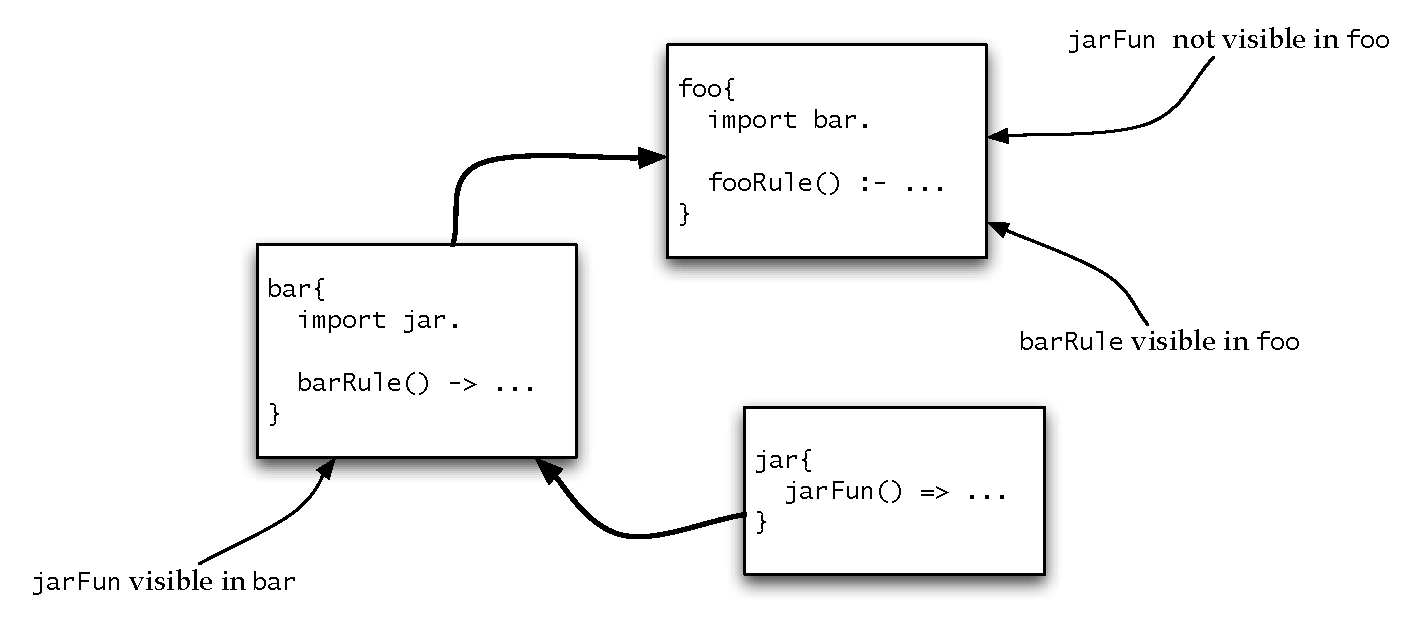
\includegraphics[width=\textwidth]{packages}
\end{boxed}
\caption{\label{program:packages:imports}A three-way package \q{import}}
\end{figure}
In this scenario \q{jarFun} is available within the \q{bar} package, but not in the \q{foo} package -- even though loading the \q{foo} package will cause \q{jar} to be loaded. If \q{jarFun} is required directly within the \q{foo} then it will have to be explicitly \q{import}ed by the \q{foo} package. Of course, the \q{barRule} action procedure is available within the \q{foo} package.

This can become an issue for type and other definitions that are shared over many packages. In that situation, the shared definitions will need to be \q{import}ed in each context that they are required.

\section{Top-level main programs}
\label{program:top-level}
Any package can also be treated as the top-level program -- provided that the package has a definition for the single argument action procedure \q{main}. In fact, \q{main} is a reserved word in \go: if a \q{main} program is defined in a package then it \emph{must} be consistent with the type assertion:
\begin{alltt}
main:[list[string]]*
\end{alltt}

If a package is executed at the top-level, then the \q{main} program in that package is executed and given as its single argument a list of the command-line arguments specified in the execution. For example, if a package \q{foo} were mentioned as the top-level package to execute in:
\begin{alltt}
\% go foo a b c
\end{alltt}
then the package \q{foo} must have an appropriate definition for \q{main} and that action procedure is entered -- with argument the list
\begin{alltt}["a","b","c"]\end{alltt}
\begin{aside}
Since the command line arguments are passed in as \q{string}s it is common for these argument strings to be parsed before they can be used in the application proper.  

The \q{\%\%} parse expression and the \q{go.stdparse} package become handy in this situation. For example, to pass a integer value to a \go fragment, where the number comes from the command line itself, then the classic way to do this is:
\begin{alltt}
mainPackage\{
  import go.stdparse.
  
  \ldots
  main([Arg,..More]) ->
    appProg(integerOf\%\%Arg);\ldots
\}
\end{alltt}
The \q{integerOf} grammar program parses a string into a \q{integer} value (see Section~\vref{stdparse:integerOf}).

See Chapter~\vref{compile} for further information on compiling and running \go programs.
\end{aside}

\section{Standard Packages}
\index{Packages!commonly loaded package}
Much of the functionality of the \go system is encapsulated in special packages that are not automatically included in every program. By convention, all \go system packages have package names of the form: \q{go.\emph{name}}; for example, the system input/output package is called \q{go.io}. To access the standard I/O package, then, it is necessary to load the \q{go.io} package:
\begin{alltt}
\emph{yourpackage}\{
  import go.io.
  
  \ldots
\}
\end{alltt}
\begin{aside}
The reason that \q{go.io} is not automatically included in every package is that that permits non-standard I/O systems to be used - for example in embedded applications, or in systems which have to interact with file systems in special ways.
\end{aside}
The standard set of packages will vary from time to time, the current set includes the packages
\begin{description}
\item[\q{go.cell}] Implements a re-assignable resource entity.
\item[\q{go.datelib}] Implements a collection of date related functions.
\item[\q{go.dynamic}] Implements dynamic relations; relations that can be updated.
\item[\q{go.hash}] Implements a hash-table package.
\item[\q{go.io}] Implements the standard I/O package
\item[\q{go.mbox}] Implements an internal thread communication package.
%\item[\q{go.scomms}] Implements a communication interface to the SCS.
\item[\q{go.setlib}] Implements a collection of set-like functions.
\item[\q{go.sort}] Implements a sort function
\item[\q{go.stack}] Implements a shareable updatable stack package.
\item[\q{go.queue}] Implements a shareable updatable queue package.
\item[\q{go.stdlib}] The standard \go language support package.\footnote{This package \emph{is automatically loaded} as it is required for successful execution of any \go program.}
\item[\q{go.stdparse}] Implements a range of parsing functions, allowing the conversion of strings to numbers, for example.
\item[\q{go.unit}] Implements a unit-testing framework.
\item[\q{go.xml}] Implements an XML parser and displayer package. Also defines the \go version of the DOM (Document Object Model).
\item[\q{go.http}] Implements many of the functions needed to build a Web server or an HTTP client.
\end{description}






\backmatter
\bibliographystyle{alpha}
\bibliography{../LogicBib}

% To generate the glossary do:
% latex letsgo
% makeindex letsgo.glo -s nomencl.ist -o letsgo.gls 
% latex letsgo (a few more times)
\cleardoublepage
\renewcommand{\nomname}{Glossary}
\renewcommand{\nompreamble}{\addcontentsline{toc}{chapter}{Glossary}\label{glossary}}
\markboth{\MakeUppercase\nomname}{\MakeUppercase\nomname}
\printglossary[1.5in]
\cleardoublepage
\printindex
\end{document}
